\documentclass[a4paper]{article}

\usepackage[left=2cm, right=2cm, top=3cm, bottom=3cm]{geometry}
\usepackage[T1]{fontenc}
\usepackage{hyperref}
\usepackage{bookmark}
\usepackage{float}
\usepackage[linesnumbered,ruled,vlined]{algorithm2e}
\hypersetup{
    linktoc=all,
    linkcolor=blue,
    colorlinks=true
}
\usepackage{amsmath}
\usepackage{float}
\usepackage{graphicx}
\usepackage{subcaption}
\restylefloat{figure}

\usepackage[polish]{babel}
\usepackage{tocloft}

\title{Imagy}
\title{
    Imagy\\ \large 
    Aplikacja do przetwarzania obrazów \\
    Dokumentacja}
\author{Paweł Pozorski}
\date{March 18, 2025}

\begin{document}

\maketitle
\begin{abstract}
    Aplikacja do przetwarzania obrazów, pozwalająca na zastosowanie różnych filtrów oraz analizę histogramu i rzutów. Zaimplementowana w SwiftUI, wspiera dowlone urządzenie z iOS w wersji 16.0+.
\end{abstract}

\newpage
\tableofcontents
\newpage

\section{Wstęp}

Poniżej opisany projekt jest aplikacją na iOS pozwalającą na zabawę z podstawowymi filtrami graficznymi. Pozwala na odczyt i zapis obrazów z galerri urządzenia, a następnie nakładanie na obraz jednego z kilkunastu wspieranych najpopularniej stosowanych filtrów. Prócz porównywania wizualnego zmian w obrazie, Imagy posiada wbudowany moduł serwujący histogram rozkładu pikseli obrazu oraz jego rzuty pionowe i poziome, poszerzając możliwości analizy zmian wprowadzonych przez transformacje o te 3 obszary.

Imagy jest aplikacją napisaną w Switft, ze wsparciem SwiftUI oraz pakietu SwiftImage. Wspiera wszystkie urządzenia iOS 16.0+ oraz niedawno wydany iPadOS. Została przetestowana na iPhone 16 oraz iPadzie Air w pionowym ustawieniu urządzenia. Aplikacja wymaga od urzytkownika dostępu do galerii by poprawnie działać.

\section{Filtry}
\label{Filtry}

Dla jasności opisu pozostawiam nazwy filtrów w oryginalnym języku angielskim. Wszelkie filtry zostały zaimplementowane w oparciu o ten sam protocol \texttt{ImagFilterProtocoleFilter}, który zawiera następujące metody i pola:

\begin{itemize}
    \item \texttt{static var name: String} - nazwa filtru.
    \item \texttt{func apply() -> Void} - przyjmuje oryginalny strumień obrazu i zwraca przetworzony.
    \item \texttt{func applyTransformation(\\to inputImage: SwiftImage.Image<SwiftImage.RGBA<UInt8>>\\) -> SwiftImage.Image<SwiftImage.RGBA<UInt8>>} - przyjmuje obraz reprezentowany przez bibliotekę SwiftImage (tj macierz 2D struktury reprezentującej piksel w RGBA) i zwraca przetworzony. Jest to metoda nadpisywana w klasach implementujących ten protocol, zawierająca właściwą implementację filtru.
    \item \texttt{func applyKernel(\\kernel: [[Float]], to inputImage: SwiftImage.Image<SwiftImage.RGBA<UInt8>>\\) -> SwiftImage.Image<SwiftImage.RGBA<UInt8>>} - przyjmuje macierz jądra filtru oraz obraz reprezentowany przez bibliotekę SwiftImage i zwraca przetworzony obraz. Jest to metoda nadpisywana w klasach implementujących ten protocol, zawierająca właściwą implementację filtru. Jej implementacja składa się z następujących kroków:
          \begin{itemize}
              \item Kopia oryginalnego obrazu.
              \item Jądro filtru jest synchronicznie nakładane na kolejne piksele obrazu.
              \item Przypadki skrajne (tj piksele na krawędziach obrazu) - interpolacja najbliższymi sąsiednimi pikselami.
          \end{itemize}
          Implementacja wspiera filtry o parzystym wymiarze jądra, biorąc wtedy za środek filtra piksel prawy-dolny od środka macierzy jądra.
          Każdy filtr używający konwolucję nakłada ją na obraz za pomocą tej funkcji.
\end{itemize}

\subsection{Averaging}

\begin{itemize}
    \item \texttt{static var name: String = "Averaging"}
    \item \texttt{kernelSize: Int} - wymiar jądra filtru, domyślnie $3$, pobierany z widoku GUI ograniczony do wartości nieparzystych z zakresu $3-21$.
    \item \texttt{static func generateAveragingKernel(size: Int) -> [[Float]]} - generuje macierz jądra filtru o wymiarze \texttt{size}x\texttt{size} zawierającą wartości $1/(size*size)$.
    \item Celem filtru jest uśrednienie wartości pikseli w zadanym otoczeniu, używany do redukcji szumu i wygładzenia obrazu.

          \begin{figure}[H]
              \centering
              \begin{subfigure}{0.2\textwidth}
                  \centering
                  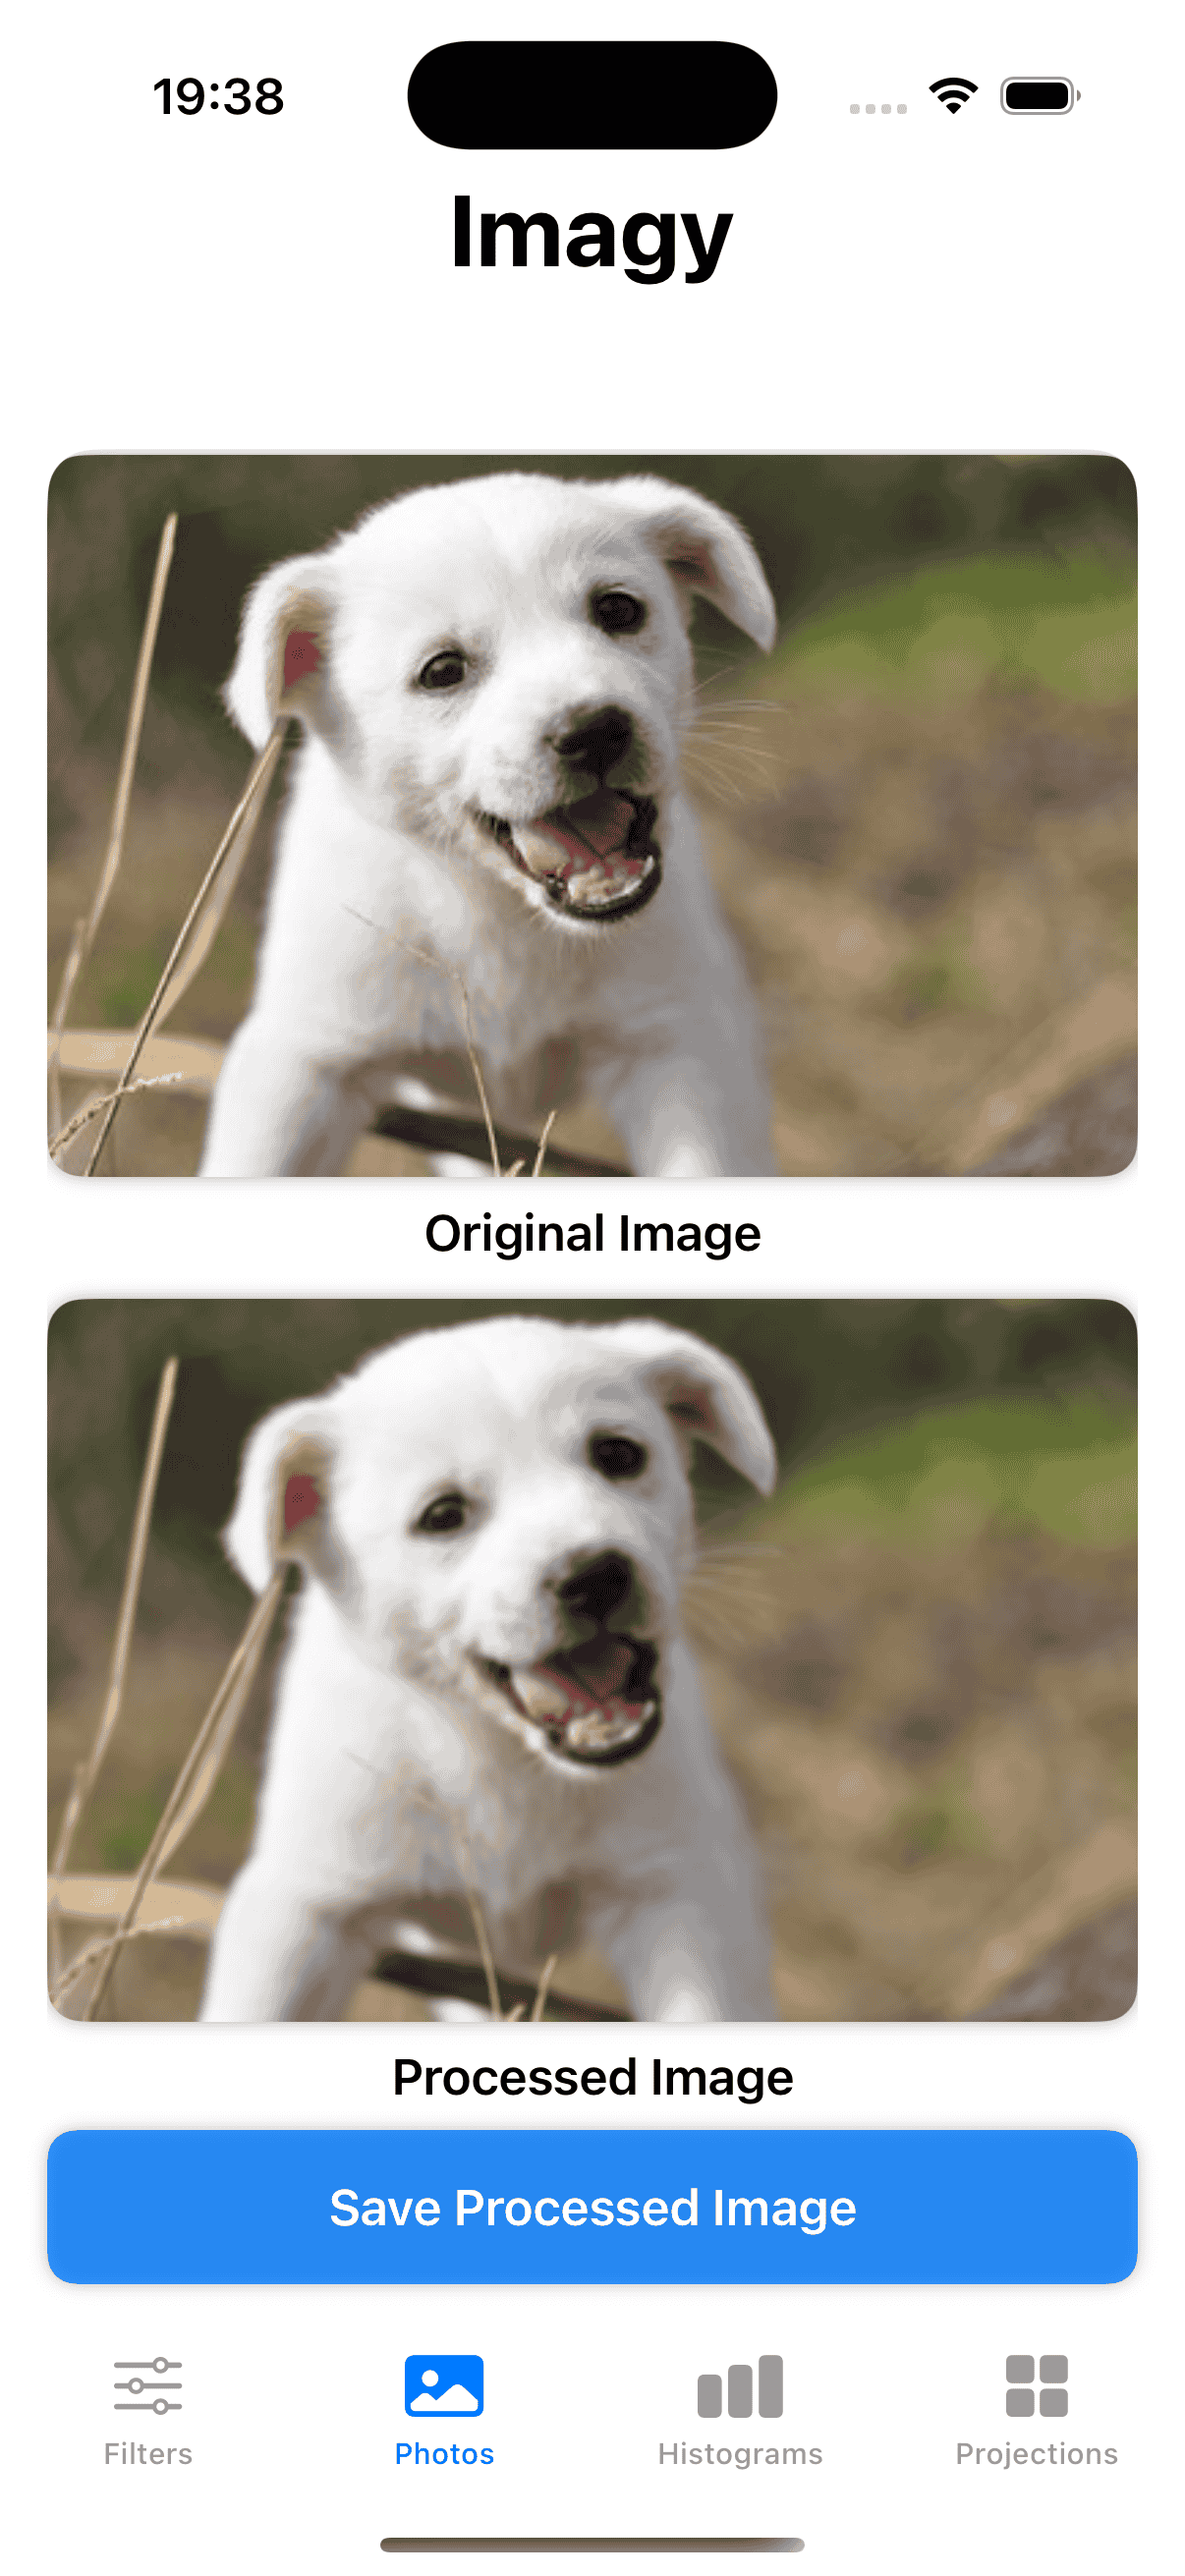
\includegraphics[width=\linewidth]{images/dog_averaging_3.png}
                  \caption{kernelSize=3}
                  \label{fig:dog_averaging_3}
              \end{subfigure}
              \hfill
              \begin{subfigure}{0.2\textwidth}
                  \centering
                  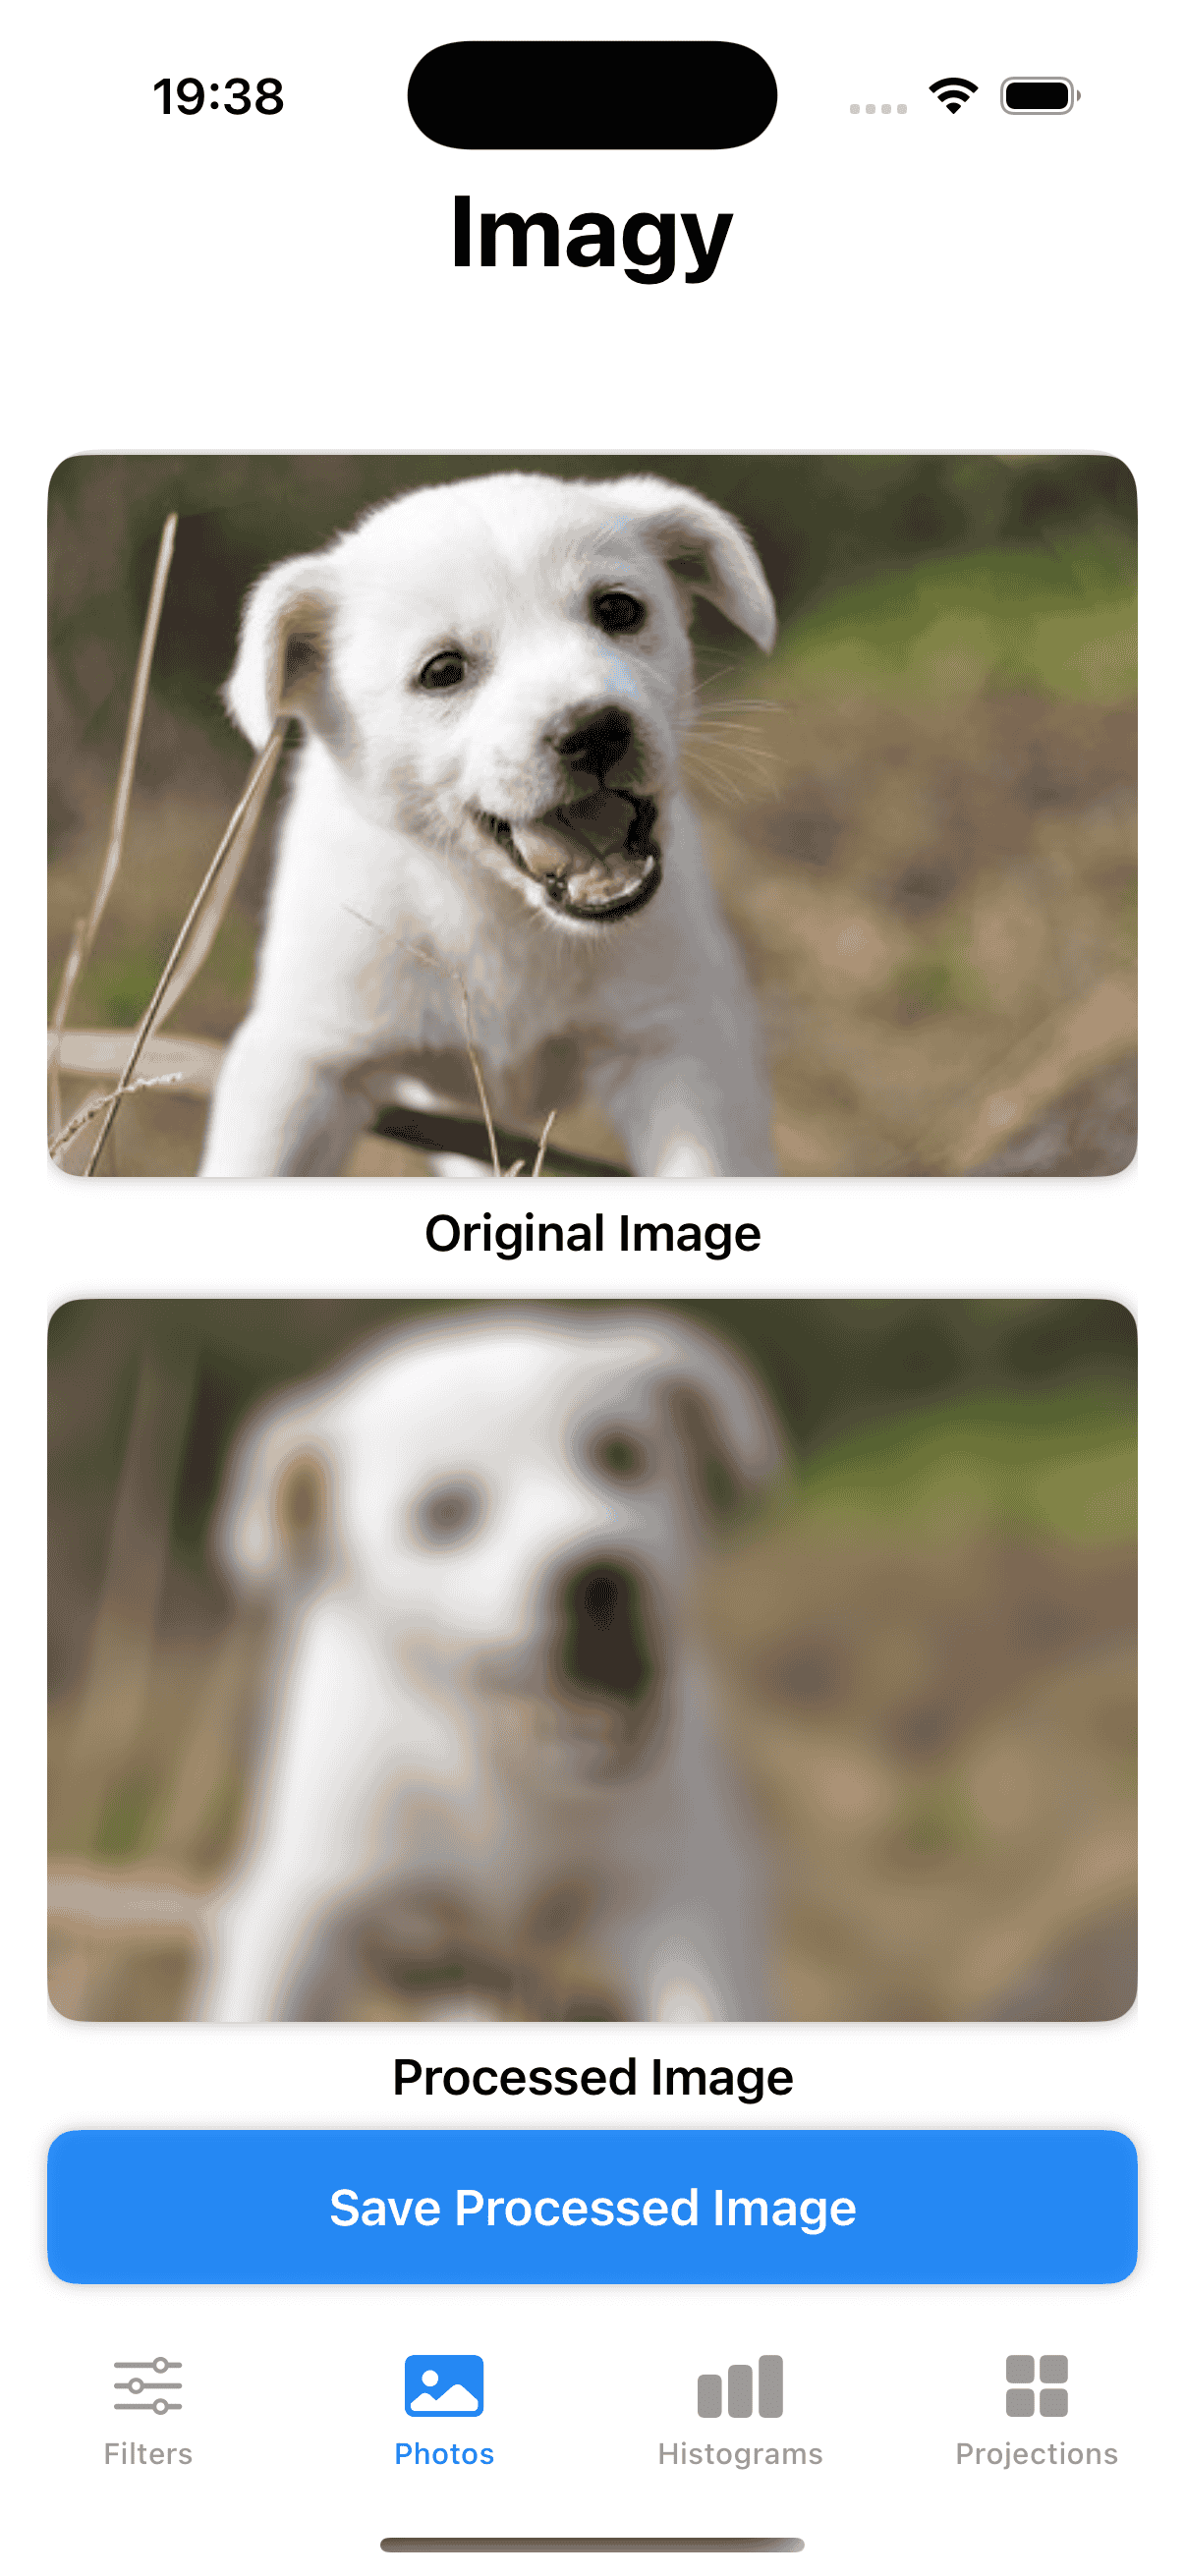
\includegraphics[width=\linewidth]{images/dog_averaging_21.png}
                  \caption{kernelSize=21}
                  \label{fig:dog_averaging_21}
              \end{subfigure}
              \hfill
              \begin{subfigure}{0.2\textwidth}
                  \centering
                  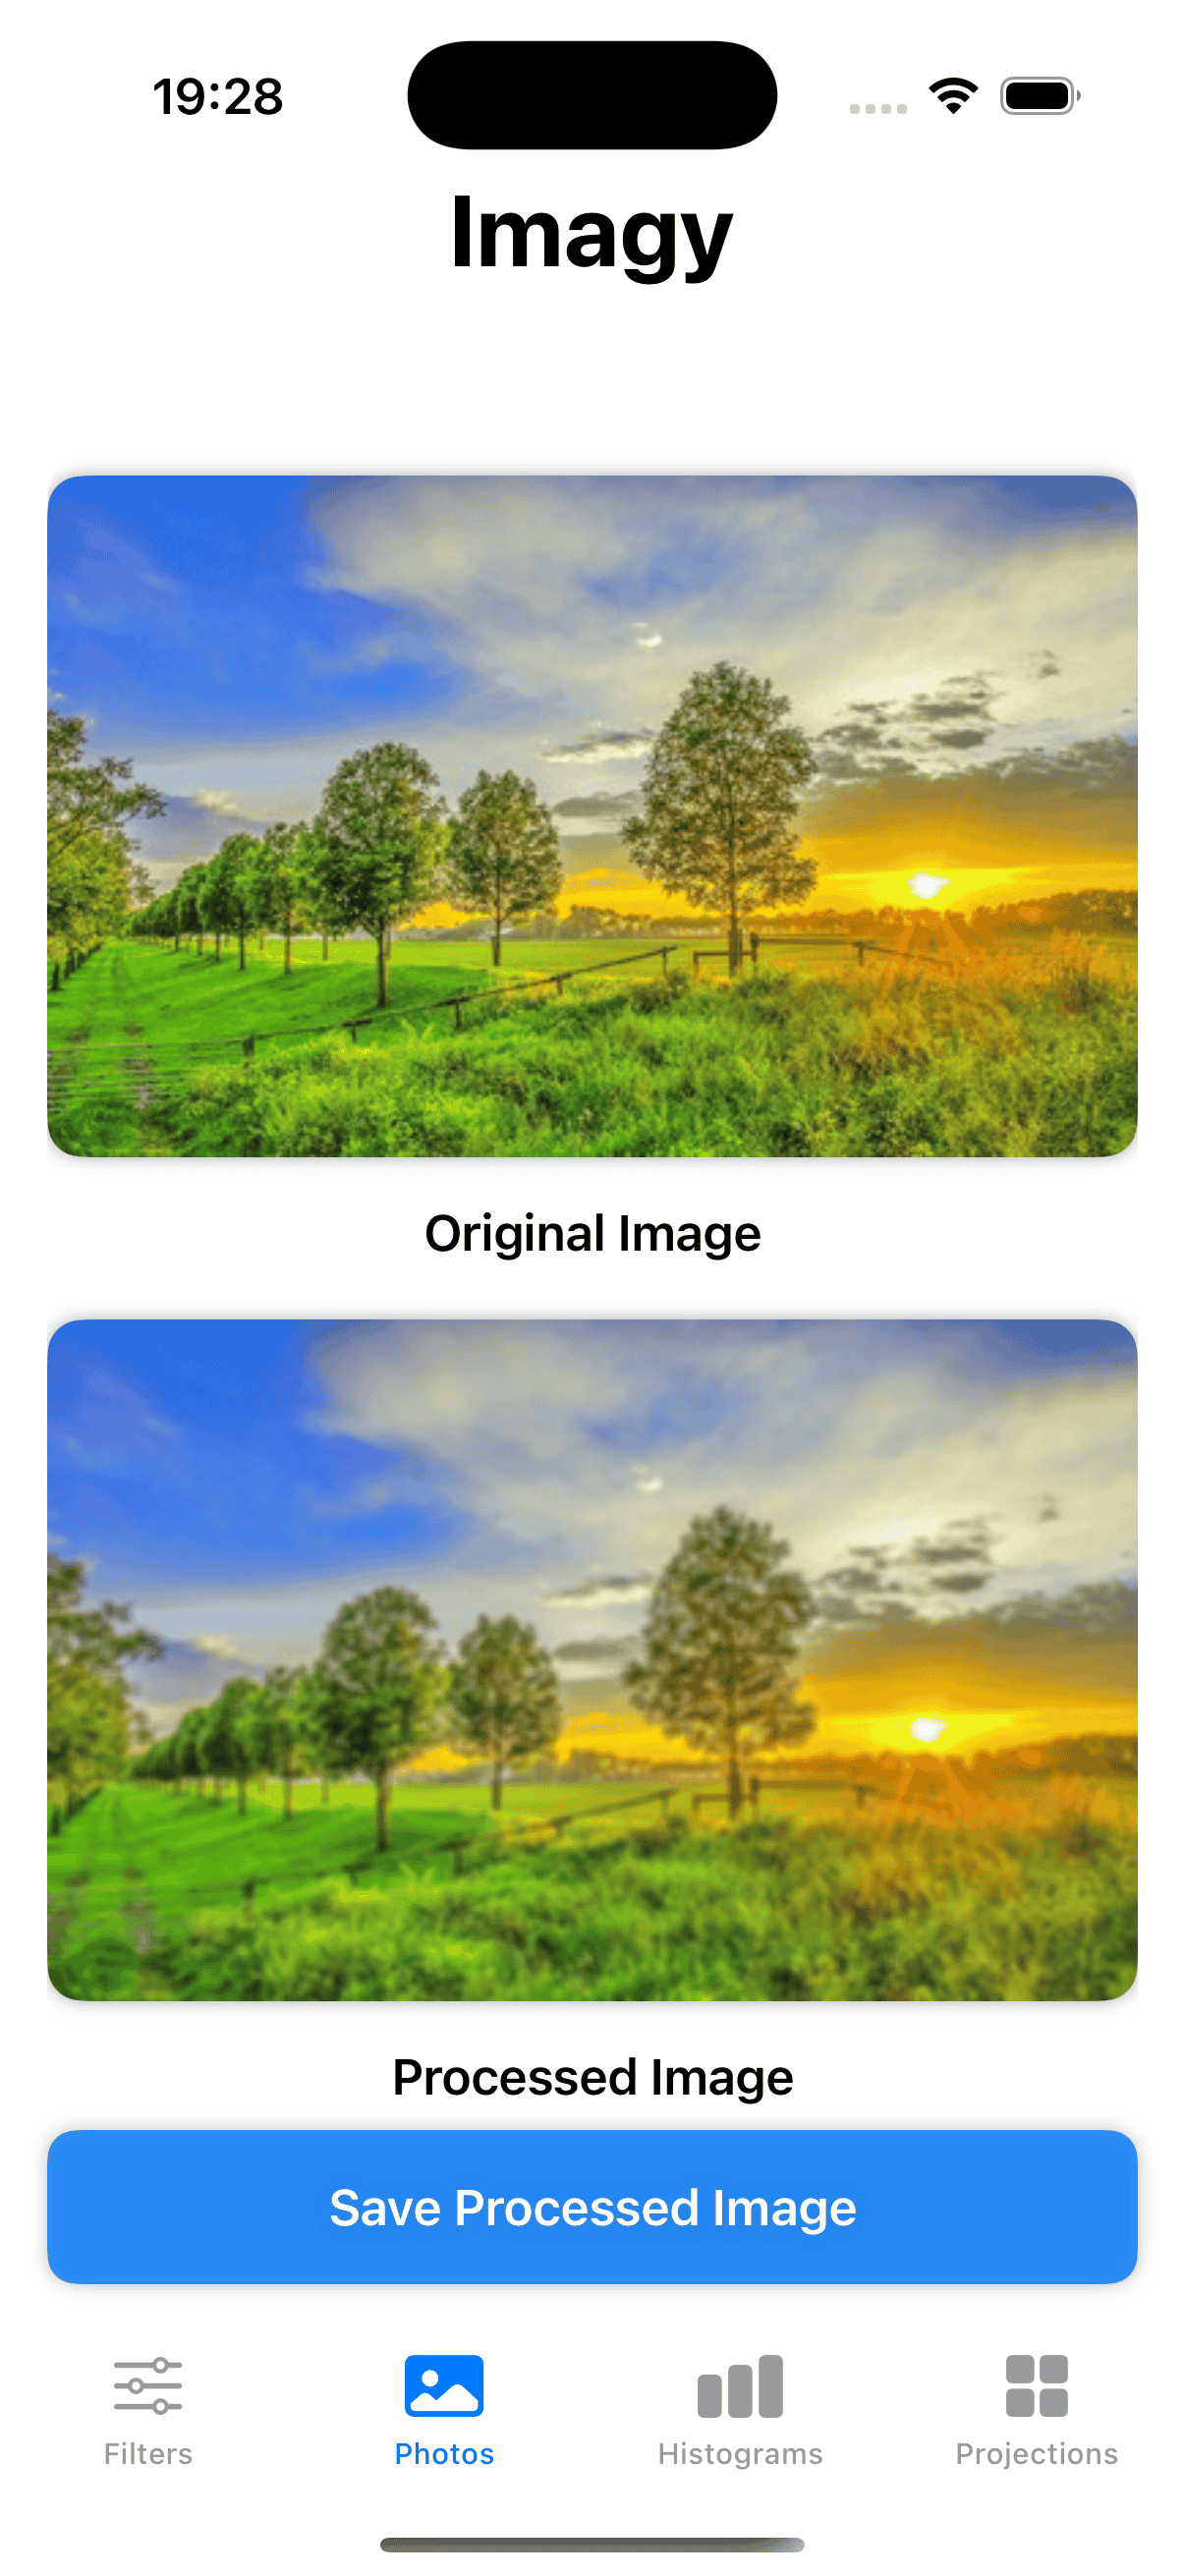
\includegraphics[width=\linewidth]{images/trees_averaging_3.png}
                  \caption{kernelSize=3}
                  \label{fig:trees_averaging_3}
              \end{subfigure}
              \hfill
              \begin{subfigure}{0.2\textwidth}
                  \centering
                  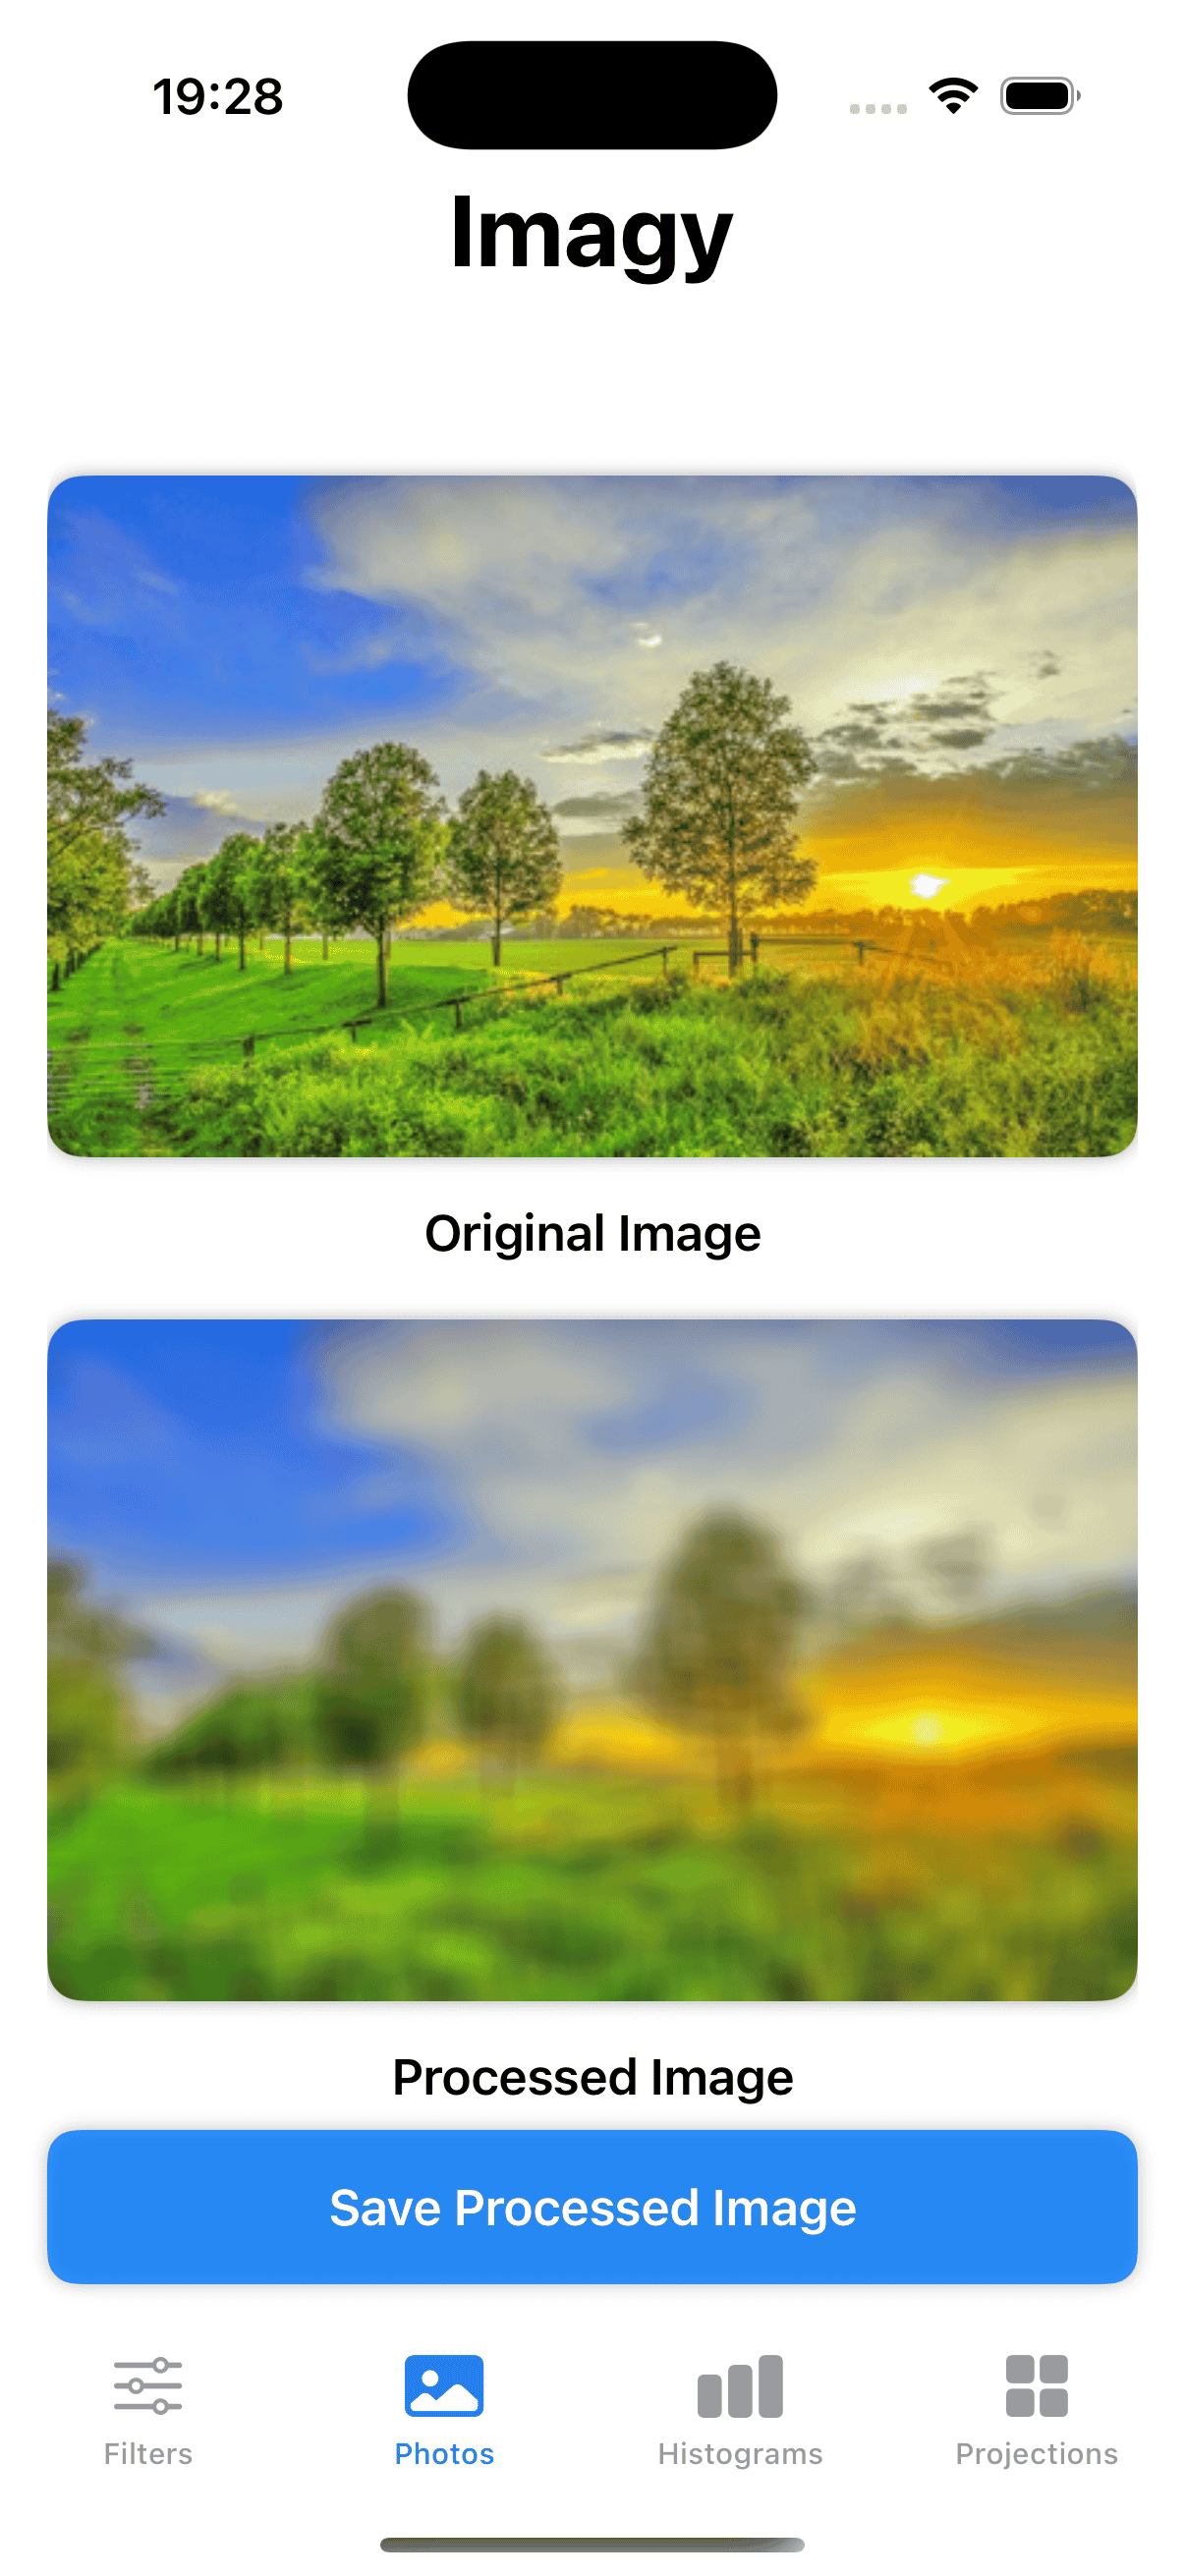
\includegraphics[width=\linewidth]{images/trees_averaging_21.png}
                  \caption{kernelSize=21}
                  \label{fig:trees_averaging_21}
              \end{subfigure}
              \caption{Averaging filter - demonstracja. Mnniejszy rozmiar kernela zakrywa niektóre detale zdjęć, pozostawia je jednak w miarę czytelne. Duży kernel (21) produkuje kompletnie rozmazany obraz.}
              \label{fig:averaging}
          \end{figure}

\end{itemize}

\subsection{Binary}

\begin{itemize}
    \item \texttt{static var name: String = "Binary"}
    \item \texttt{threshold: Int} - wartość progowa, domyślnie $128$, pobierana z widoku GUI ograniczona do zakresu $0-255$. Piksele o wartości mniejszej niż progowana są ustawiane na $0$, a większej na $1$.
    \item Filtr jest używany do wykrywania krawędzi w obrazie, segmentacji obrazu, przetwarzania obrazów w Computer Vision (np wykrywanie tekstu OCR).
\end{itemize}

\begin{figure}[H]
    \centering
    \begin{subfigure}{0.2\textwidth}
        \centering
        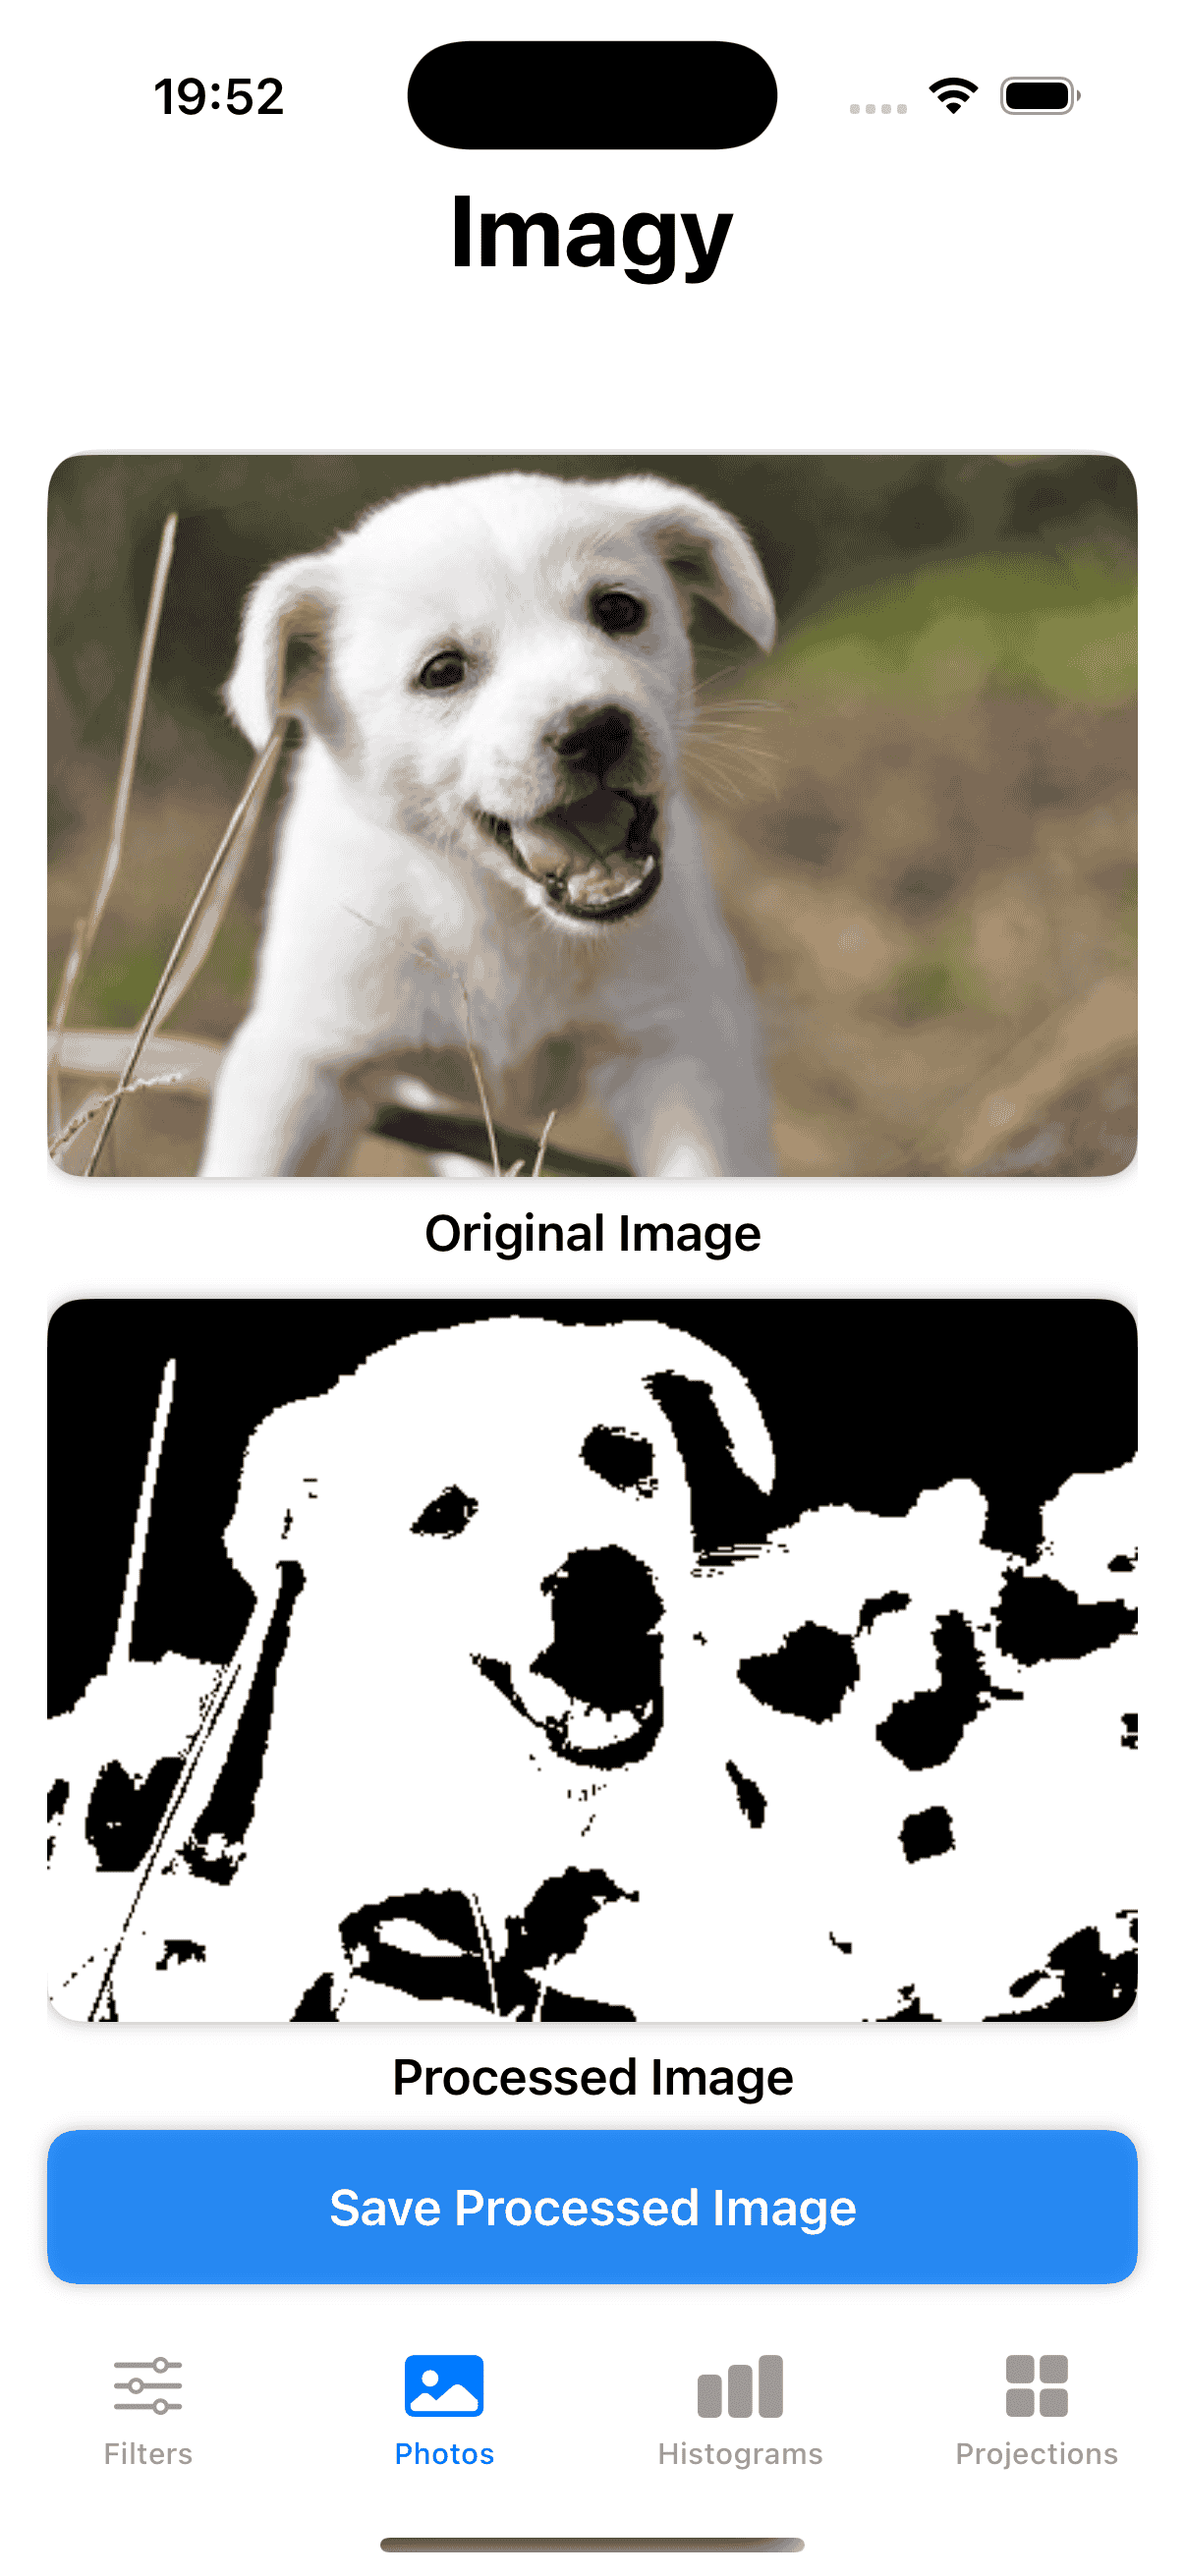
\includegraphics[width=\linewidth]{images/dog_binary_128.png}
        \caption{threshold=128}
        \label{fig:dog_binary_128}
    \end{subfigure}
    \hfill
    \begin{subfigure}{0.2\textwidth}
        \centering
        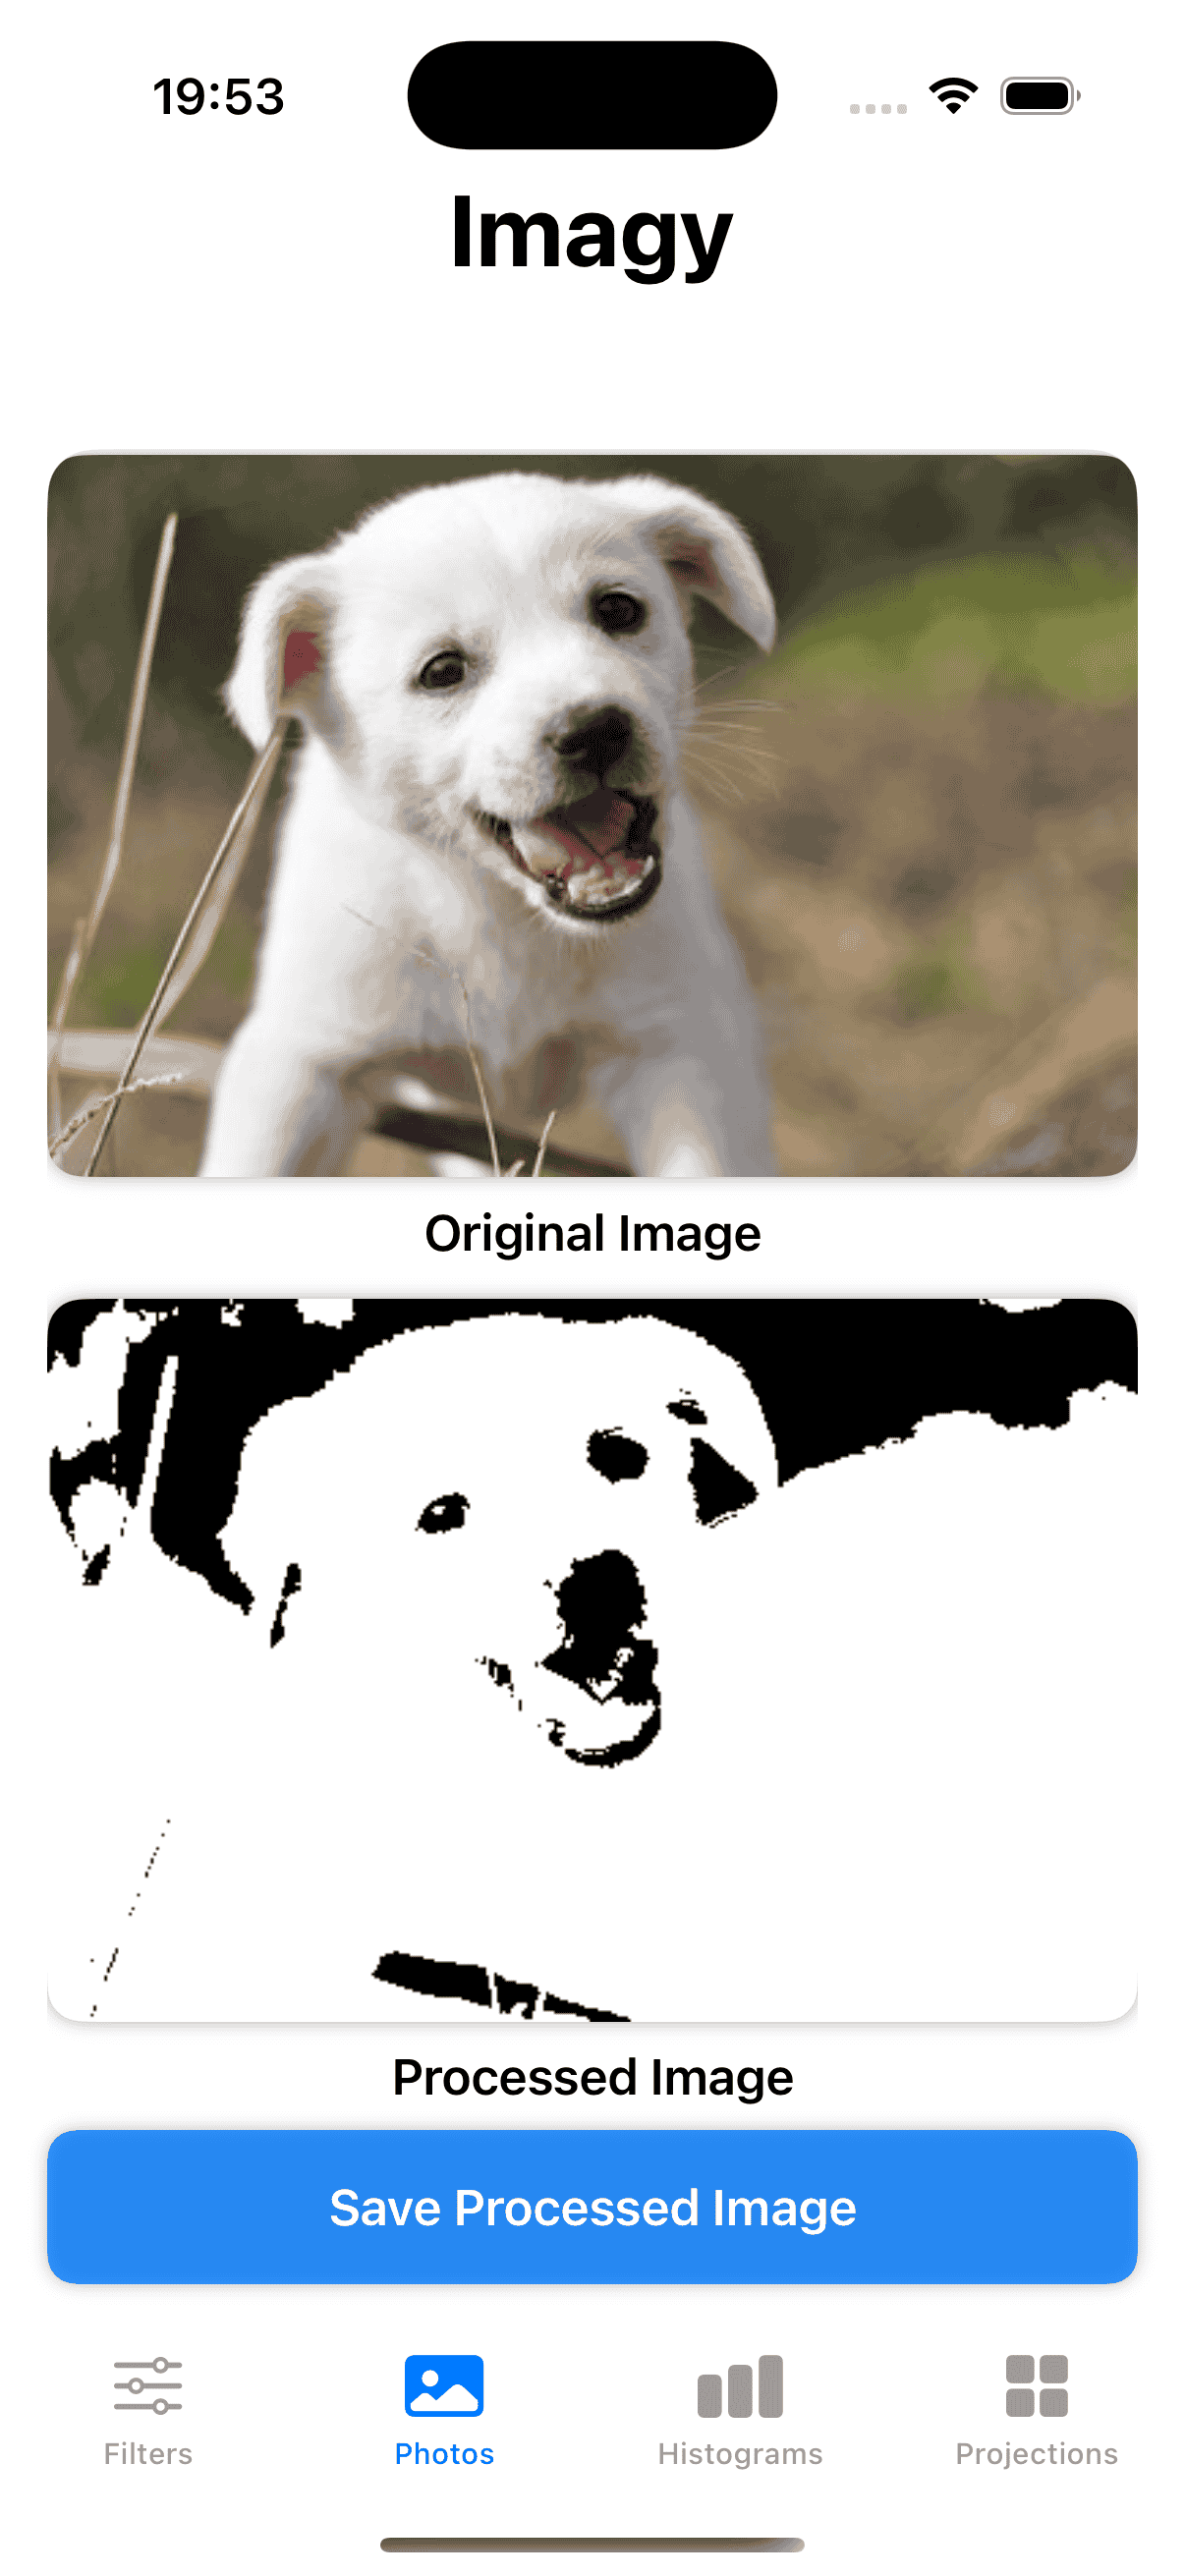
\includegraphics[width=\linewidth]{images/dog_binary_87.png}
        \caption{threshold=87}
        \label{fig:dog_binary_87}
    \end{subfigure}
    \hfill
    \begin{subfigure}{0.2\textwidth}
        \centering
        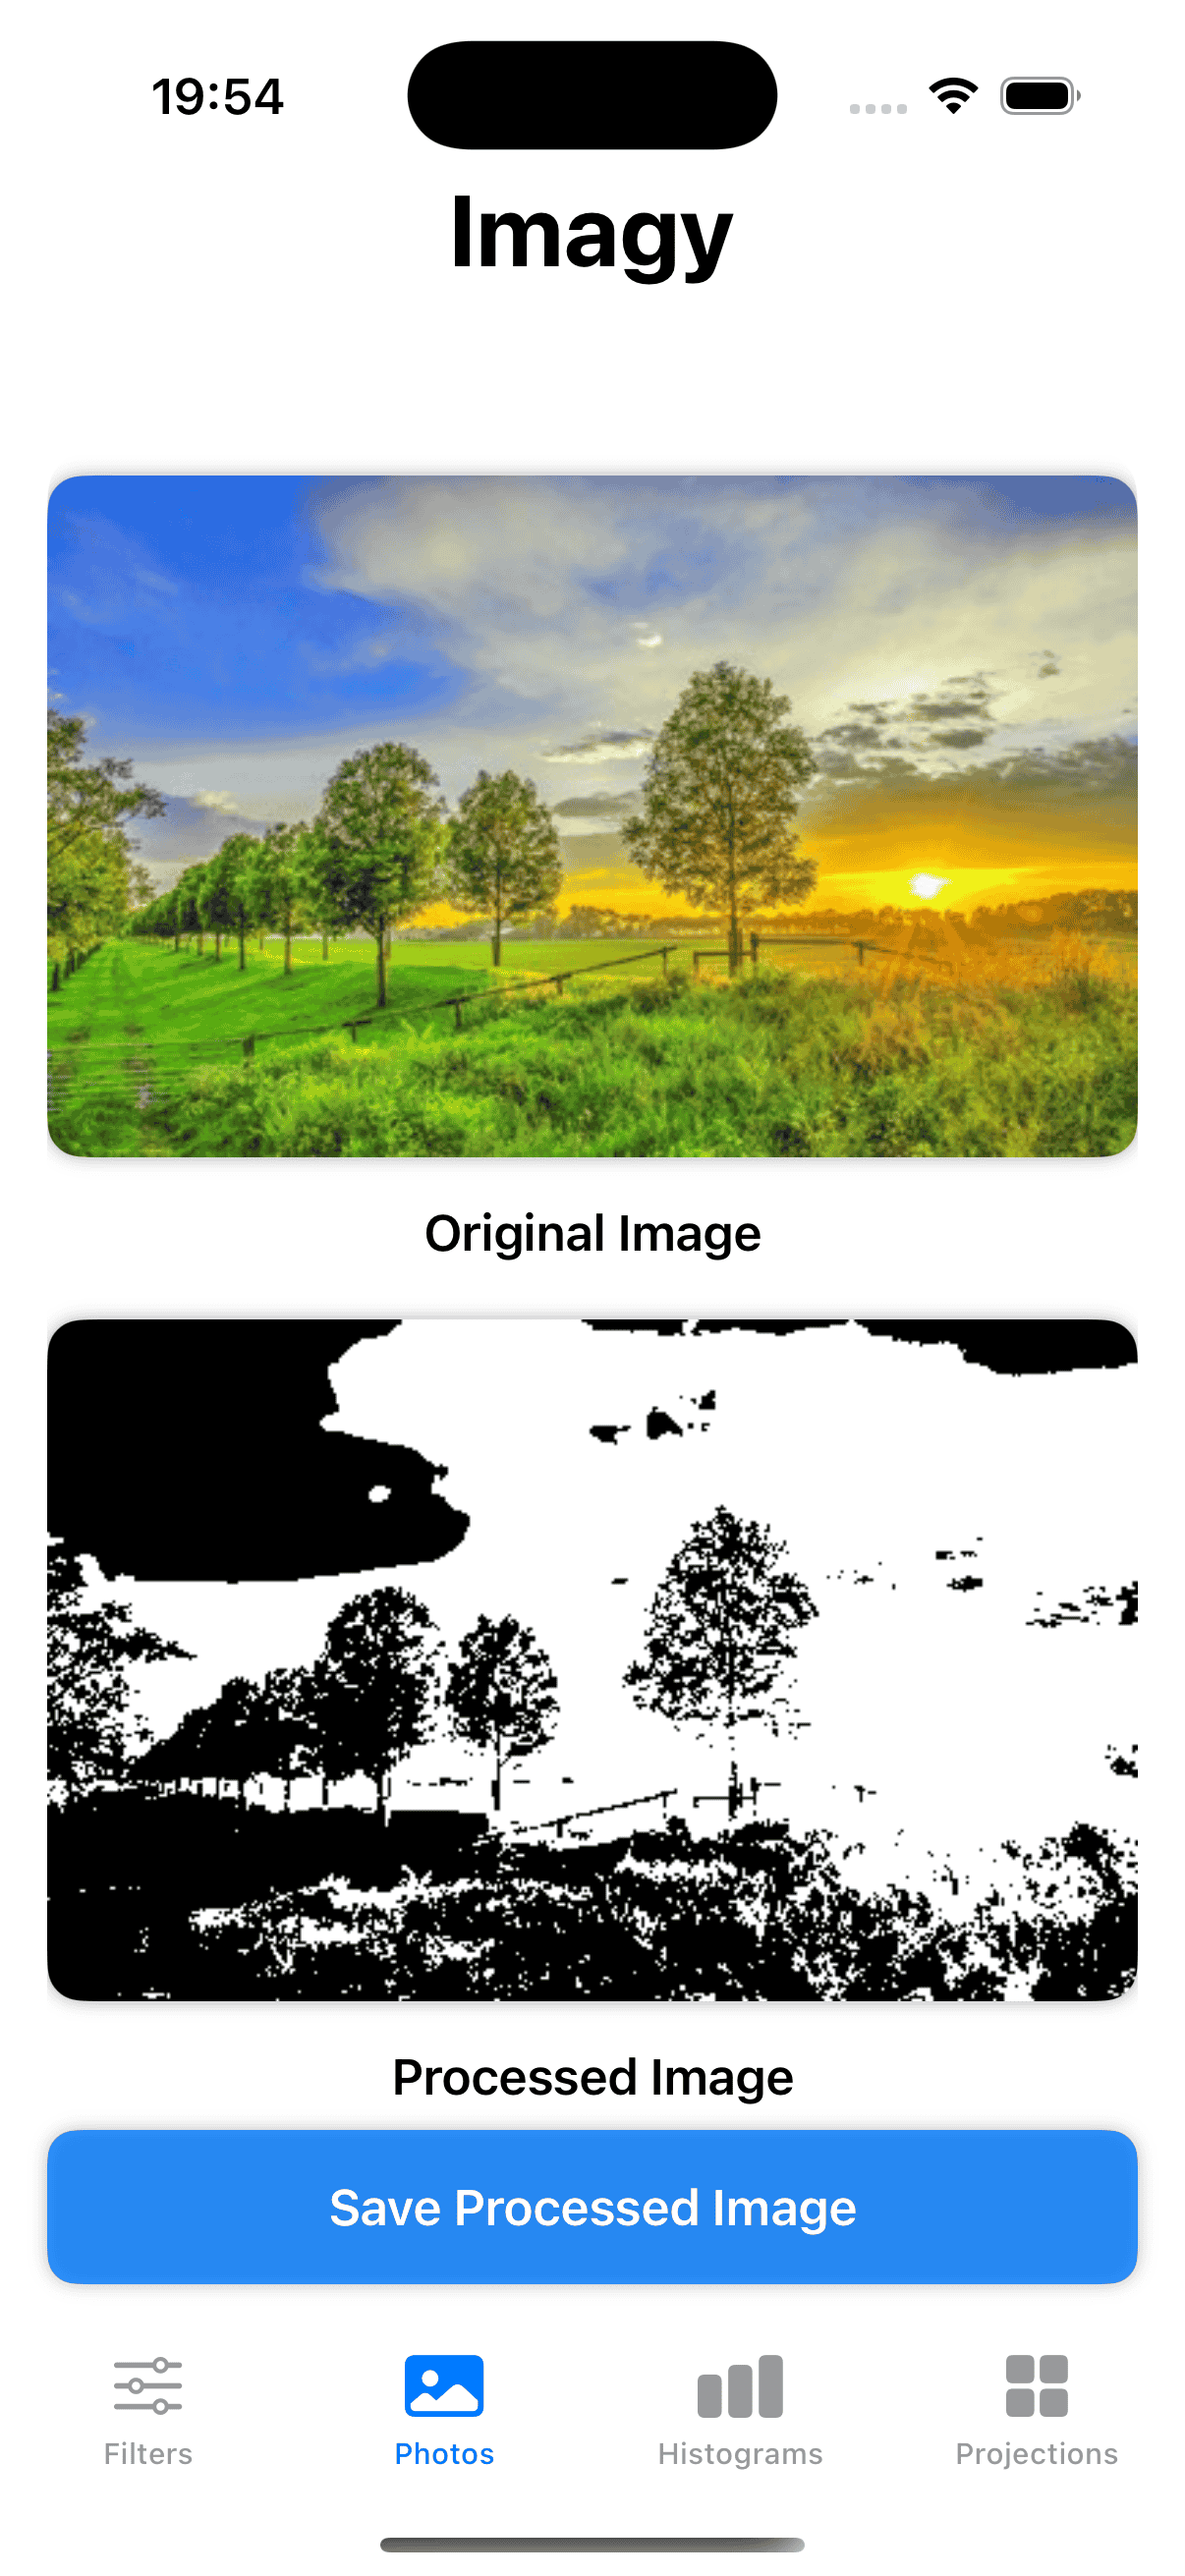
\includegraphics[width=\linewidth]{images/trees_binary_128.png}
        \caption{threshold=128}
        \label{fig:trees_binary_128}
    \end{subfigure}
    \hfill
    \begin{subfigure}{0.2\textwidth}
        \centering
        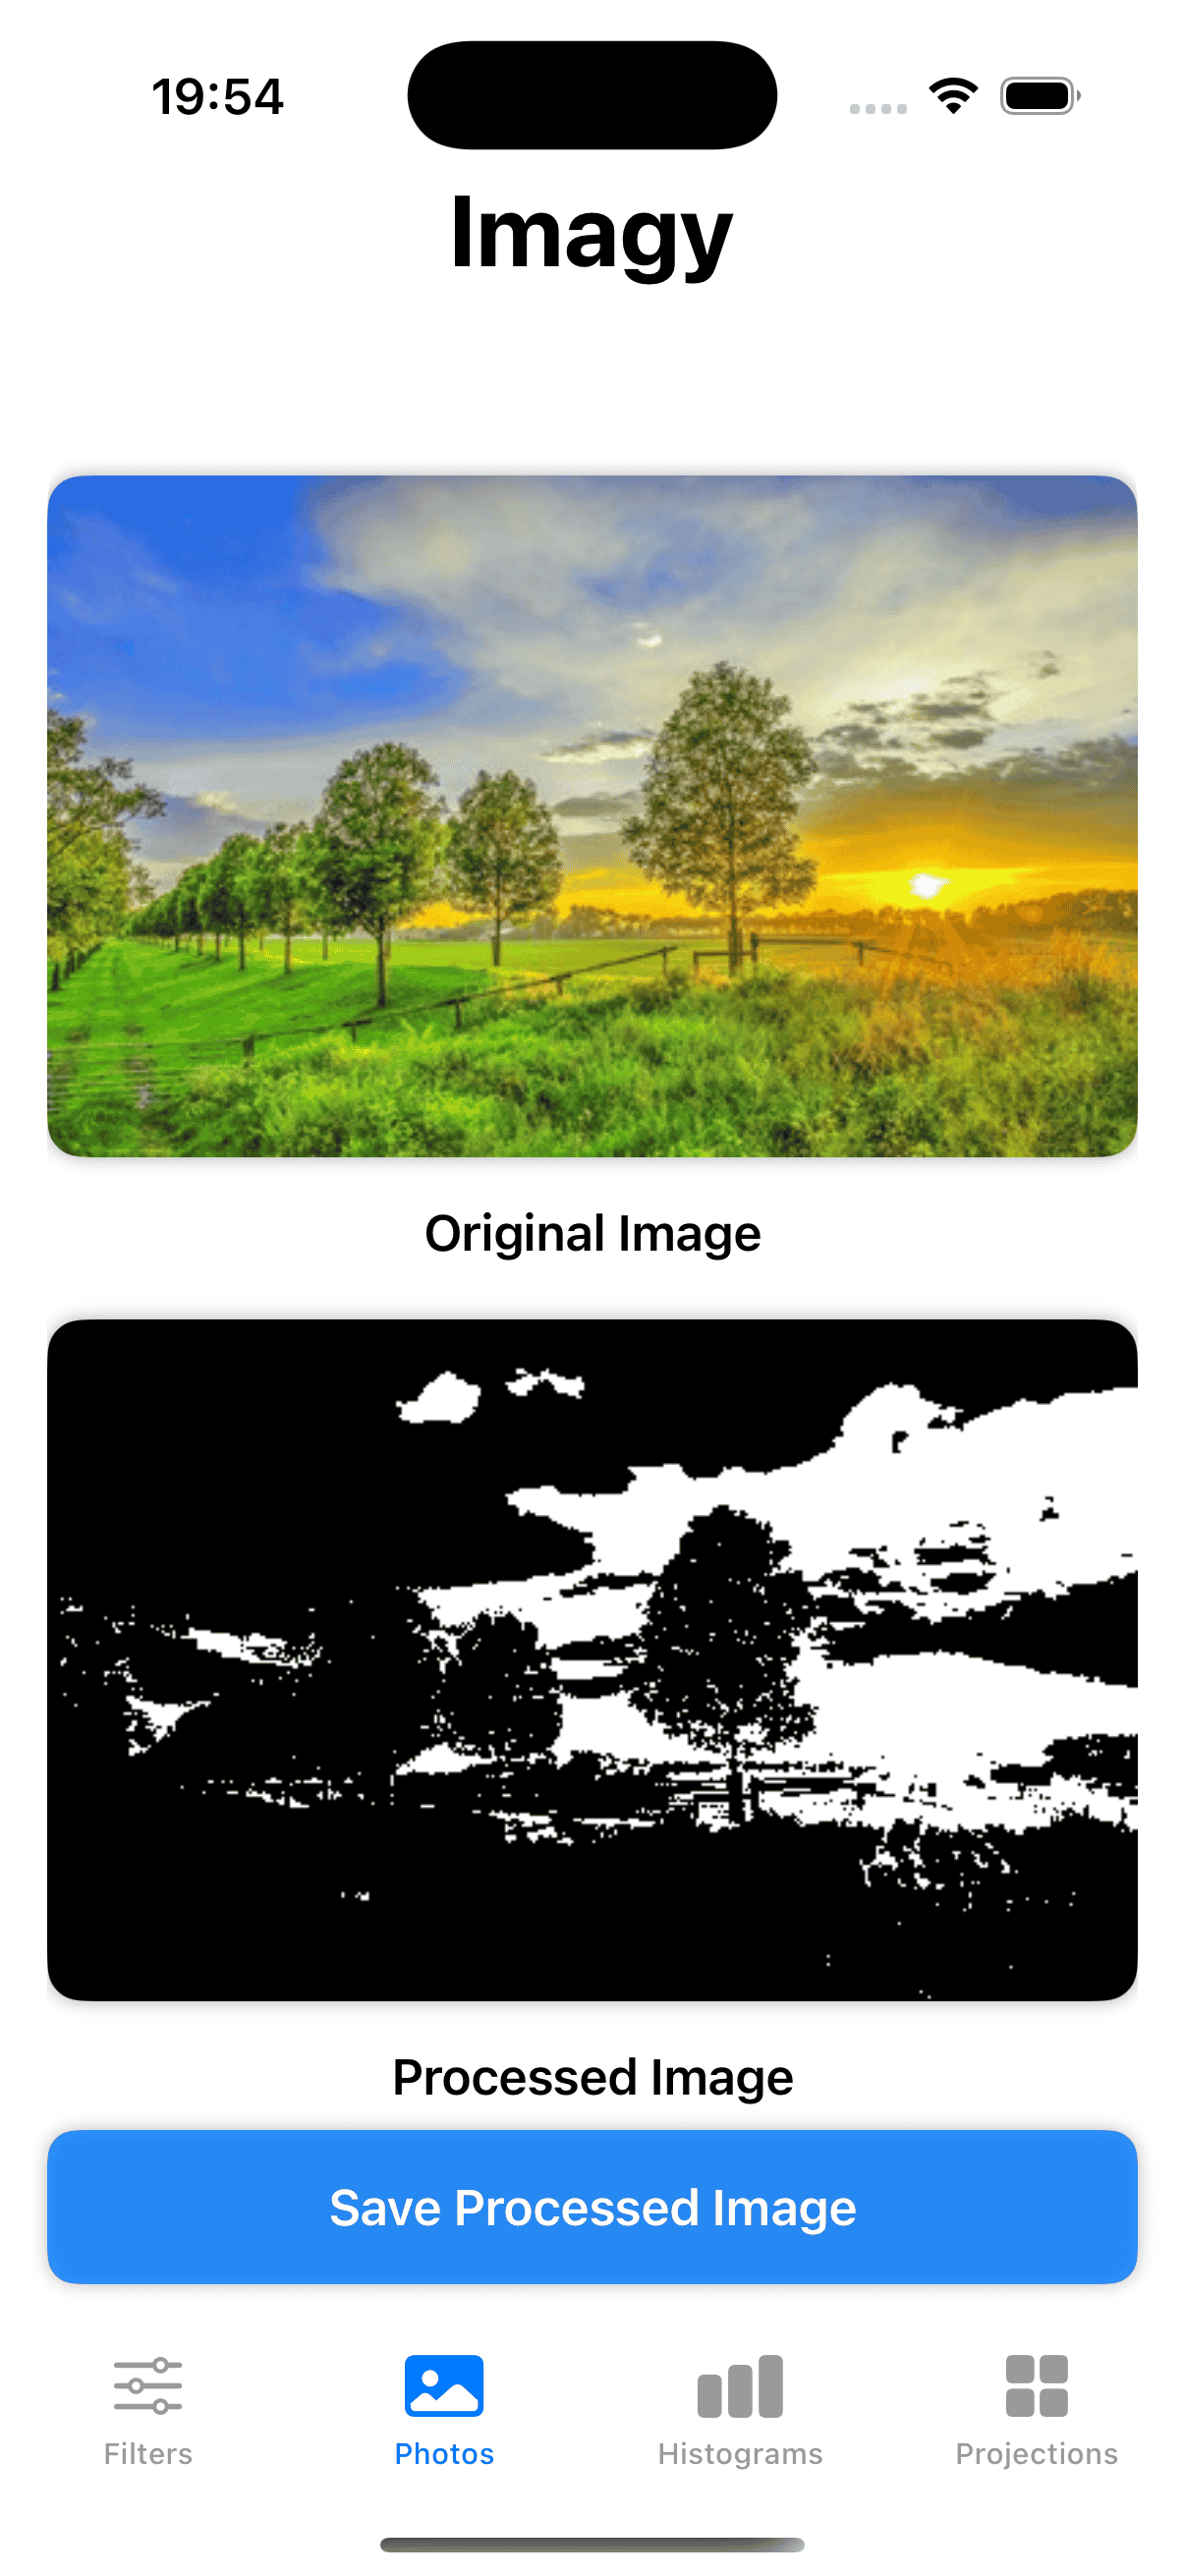
\includegraphics[width=\linewidth]{images/trees_binary_183.png}
        \caption{threshold=183}
        \label{fig:trees_binary_183}
    \end{subfigure}
    \caption{Binary filter - demonstracja. Po zdjęciu z psem widzimy że zmniejszenie thresholdu powoduje mpowanie coraz ciemniejszych obszarów na białe, w przeciwieństwie do demonstracji na prawo z drzewami - większy threshold powoduje że nawet część chmur jest mapowana na kolor czerni.}
    \label{fig:binary}
\end{figure}

\begin{figure}[H]
    \centering
    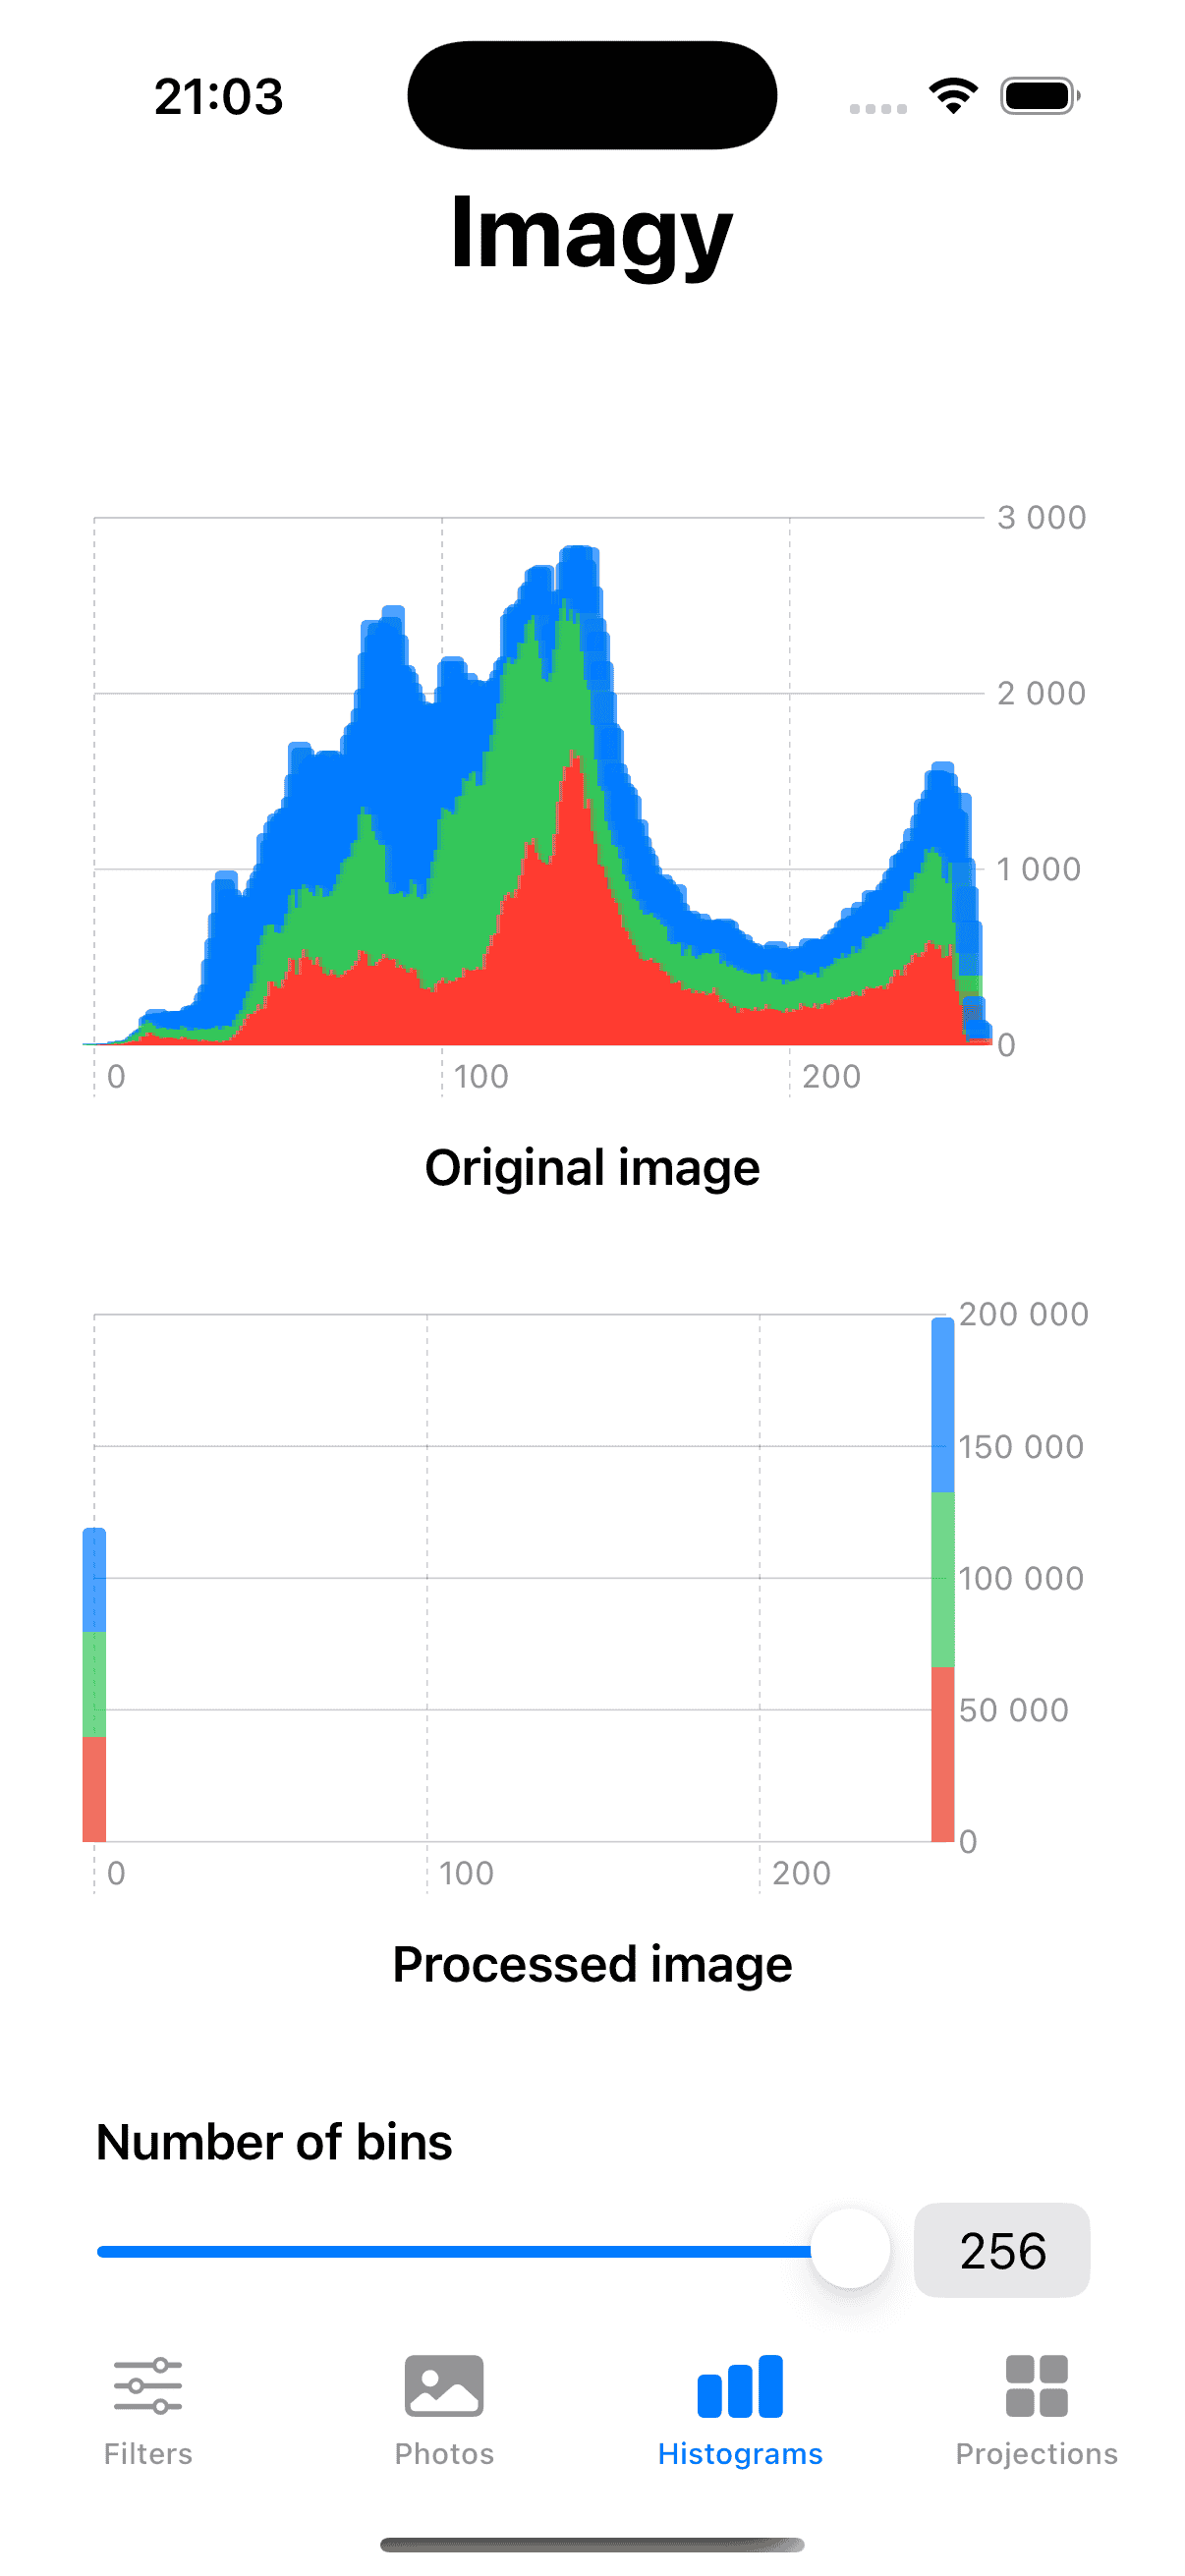
\includegraphics[width=0.25\linewidth]{images/dog_binary_histogram.png}
    \caption{Histogram for dog's binary filter with threshold=128.}
    \label{fig:dog_binary_histogram}
\end{figure}

\subsection{Brightness}

\begin{itemize}
    \item \texttt{static var name: String = "Brightness Correction"}
    \item \texttt{intensity: Int} - wartość jasności, domyślnie $50$, pobierana z widoku GUI ograniczona do zakresu $-255-255$. Do każdego piksela (kanały wszystkie prócz alfa) jest dodawana jego wartość (oczywiście potem piksel jest ograniczany do zakresu $0-255$).
    \item Filtr jest używany do poprawy niedoświetlonych / prześwietlonych obrazów, poprawy widoczności szczegółów na ciemnych obszarach oraz w Computer Vision (np wykrywanie tekstu OCR).
\end{itemize}

\begin{figure}[H]
    \centering
    \begin{subfigure}{0.2\textwidth}
        \centering
        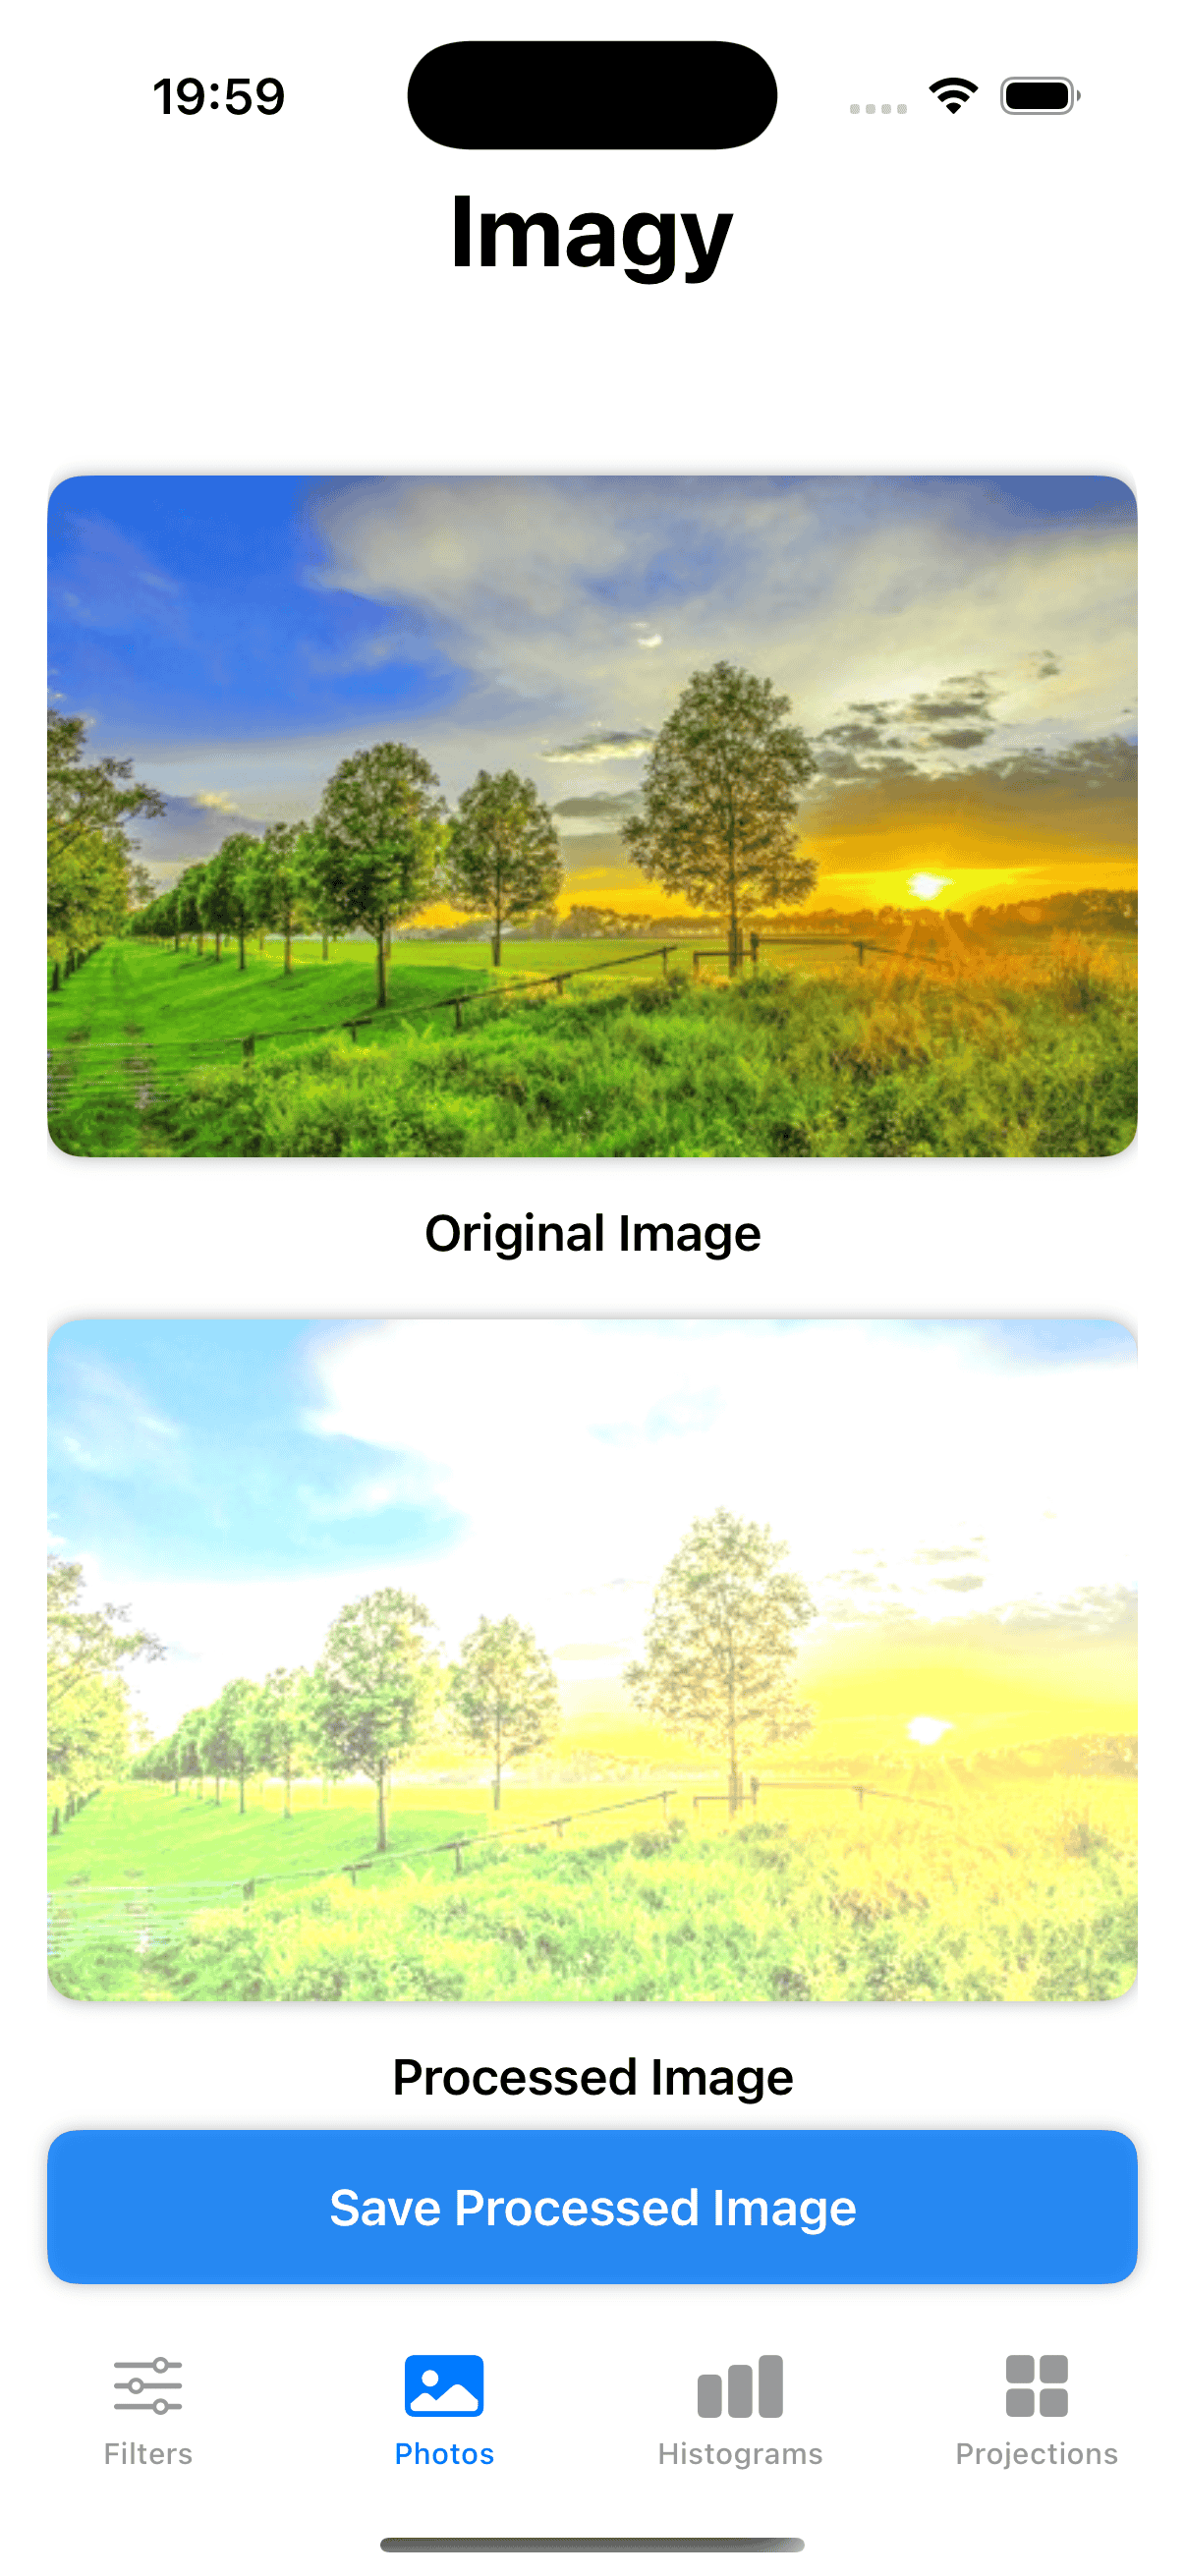
\includegraphics[width=\linewidth]{images/trees_brightness_118.png}
        \caption{intensity=118}
        \label{fig:trees_brightness_118}
    \end{subfigure}
    \begin{subfigure}{0.2\textwidth}
        \centering
        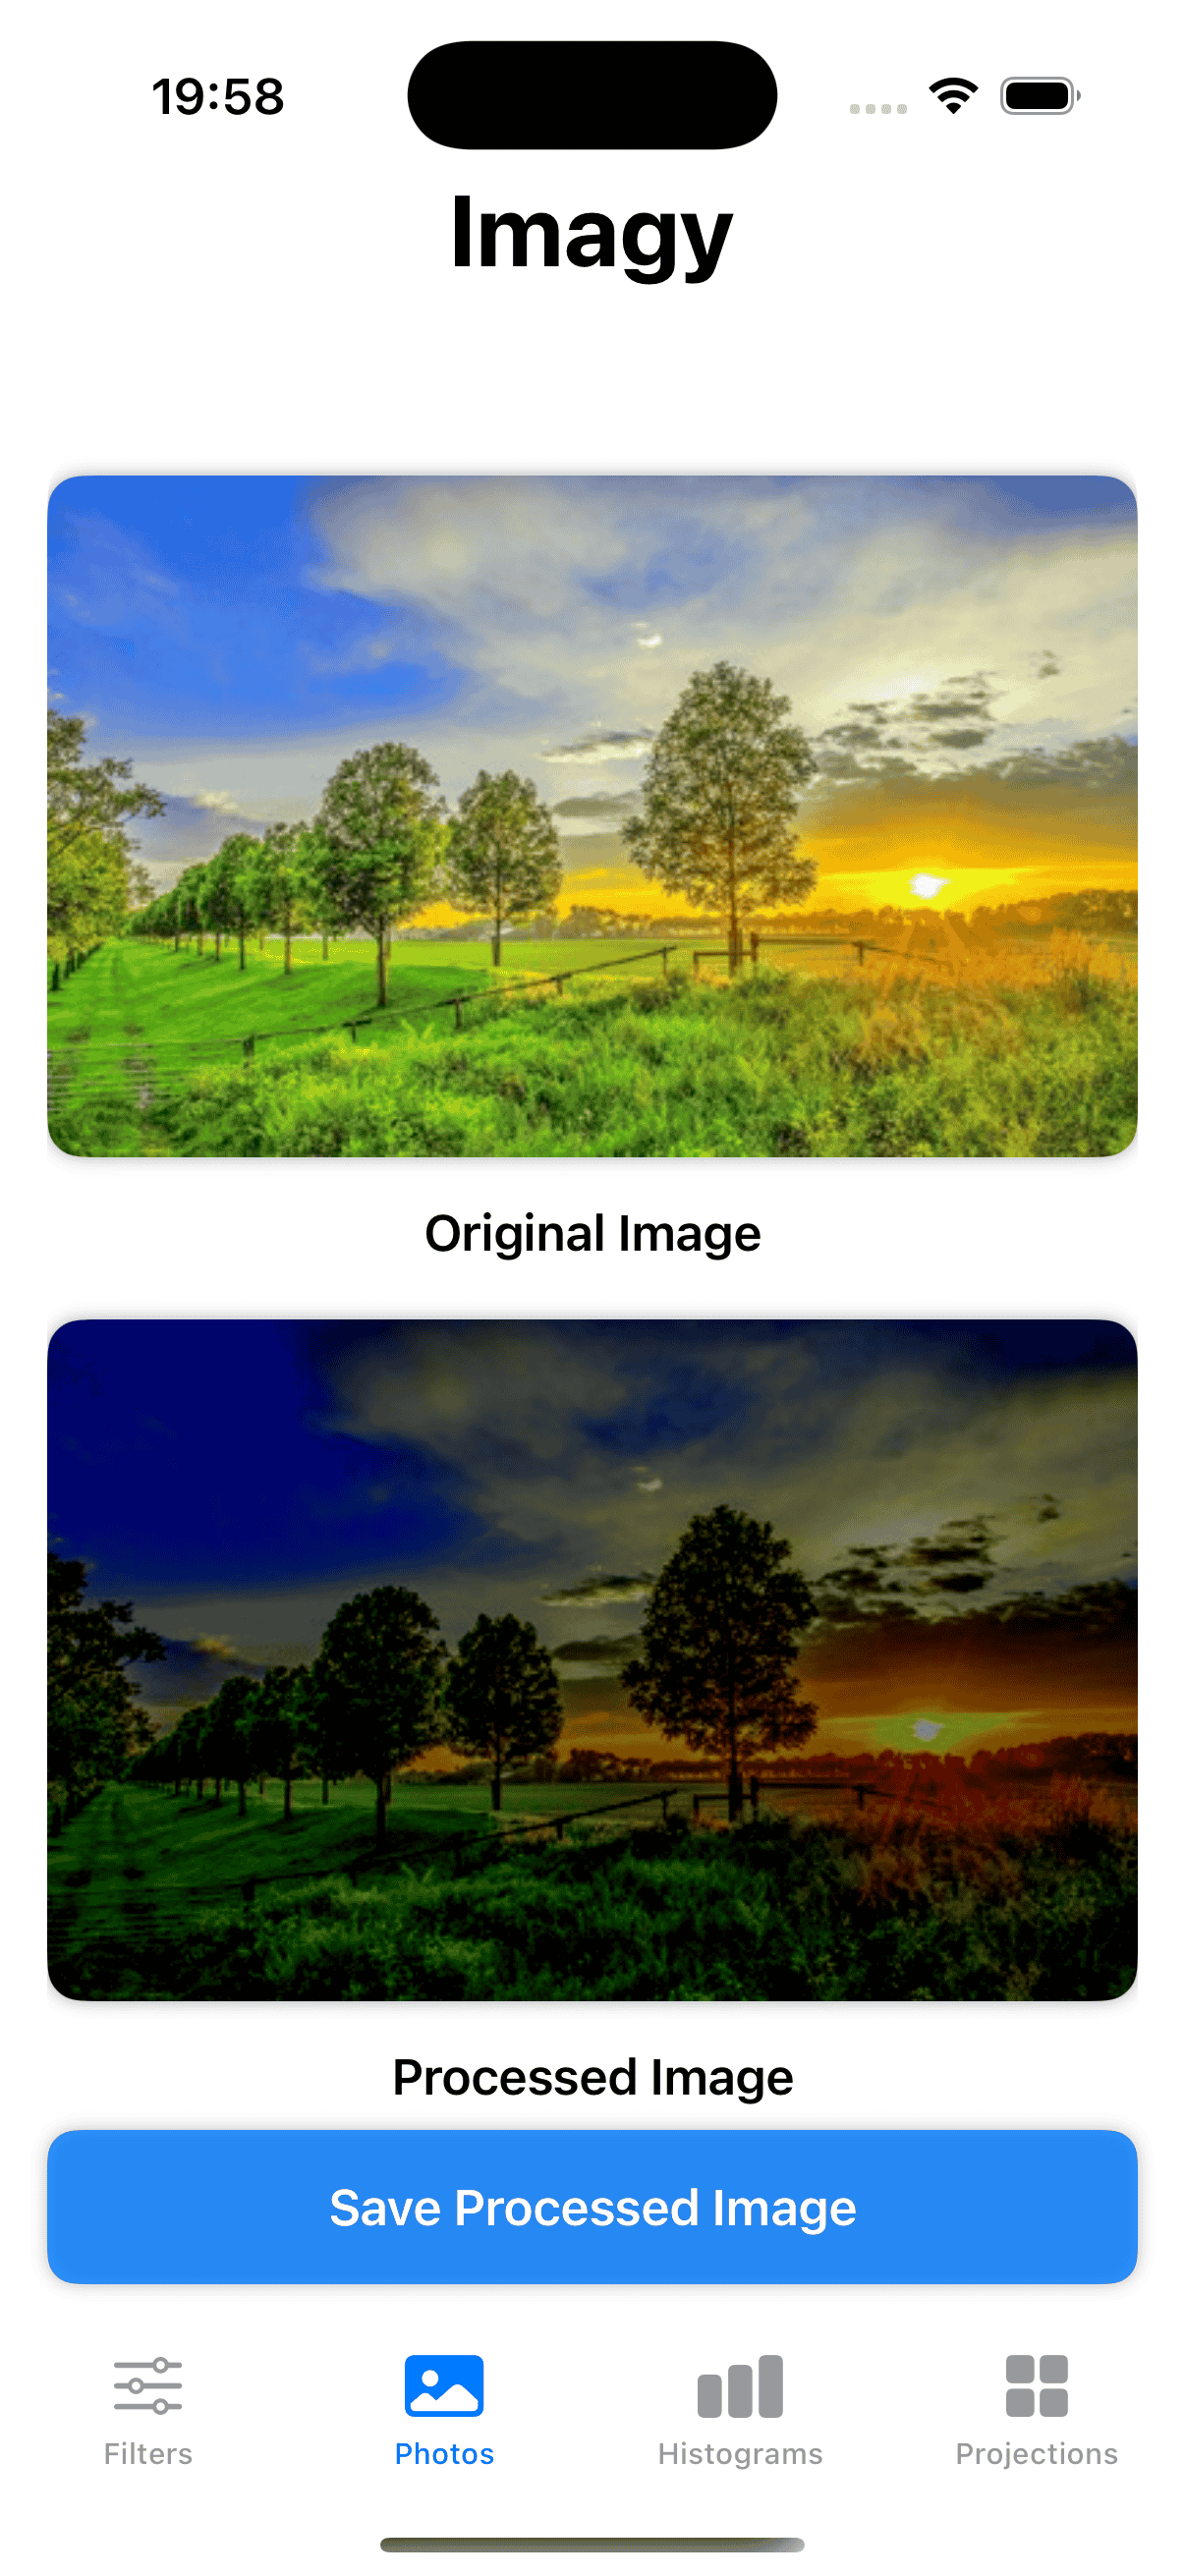
\includegraphics[width=\linewidth]{images/trees_brightness_m119.png}
        \caption{intensity=-119}
        \label{fig:trees_brightness_m119}
    \end{subfigure}
    \caption{Brightness filter - demonstracja. Intensity znacząco dodatnie produkuje obrazek mocno rozjaśniony, wręcz wyblakły. W przeciwieństwie do znacząco przyciemnionego rysunku na prawo z negatywną wartością intensity.}
    \label{fig:brightness}
\end{figure}

\begin{figure}[H]
    \centering
    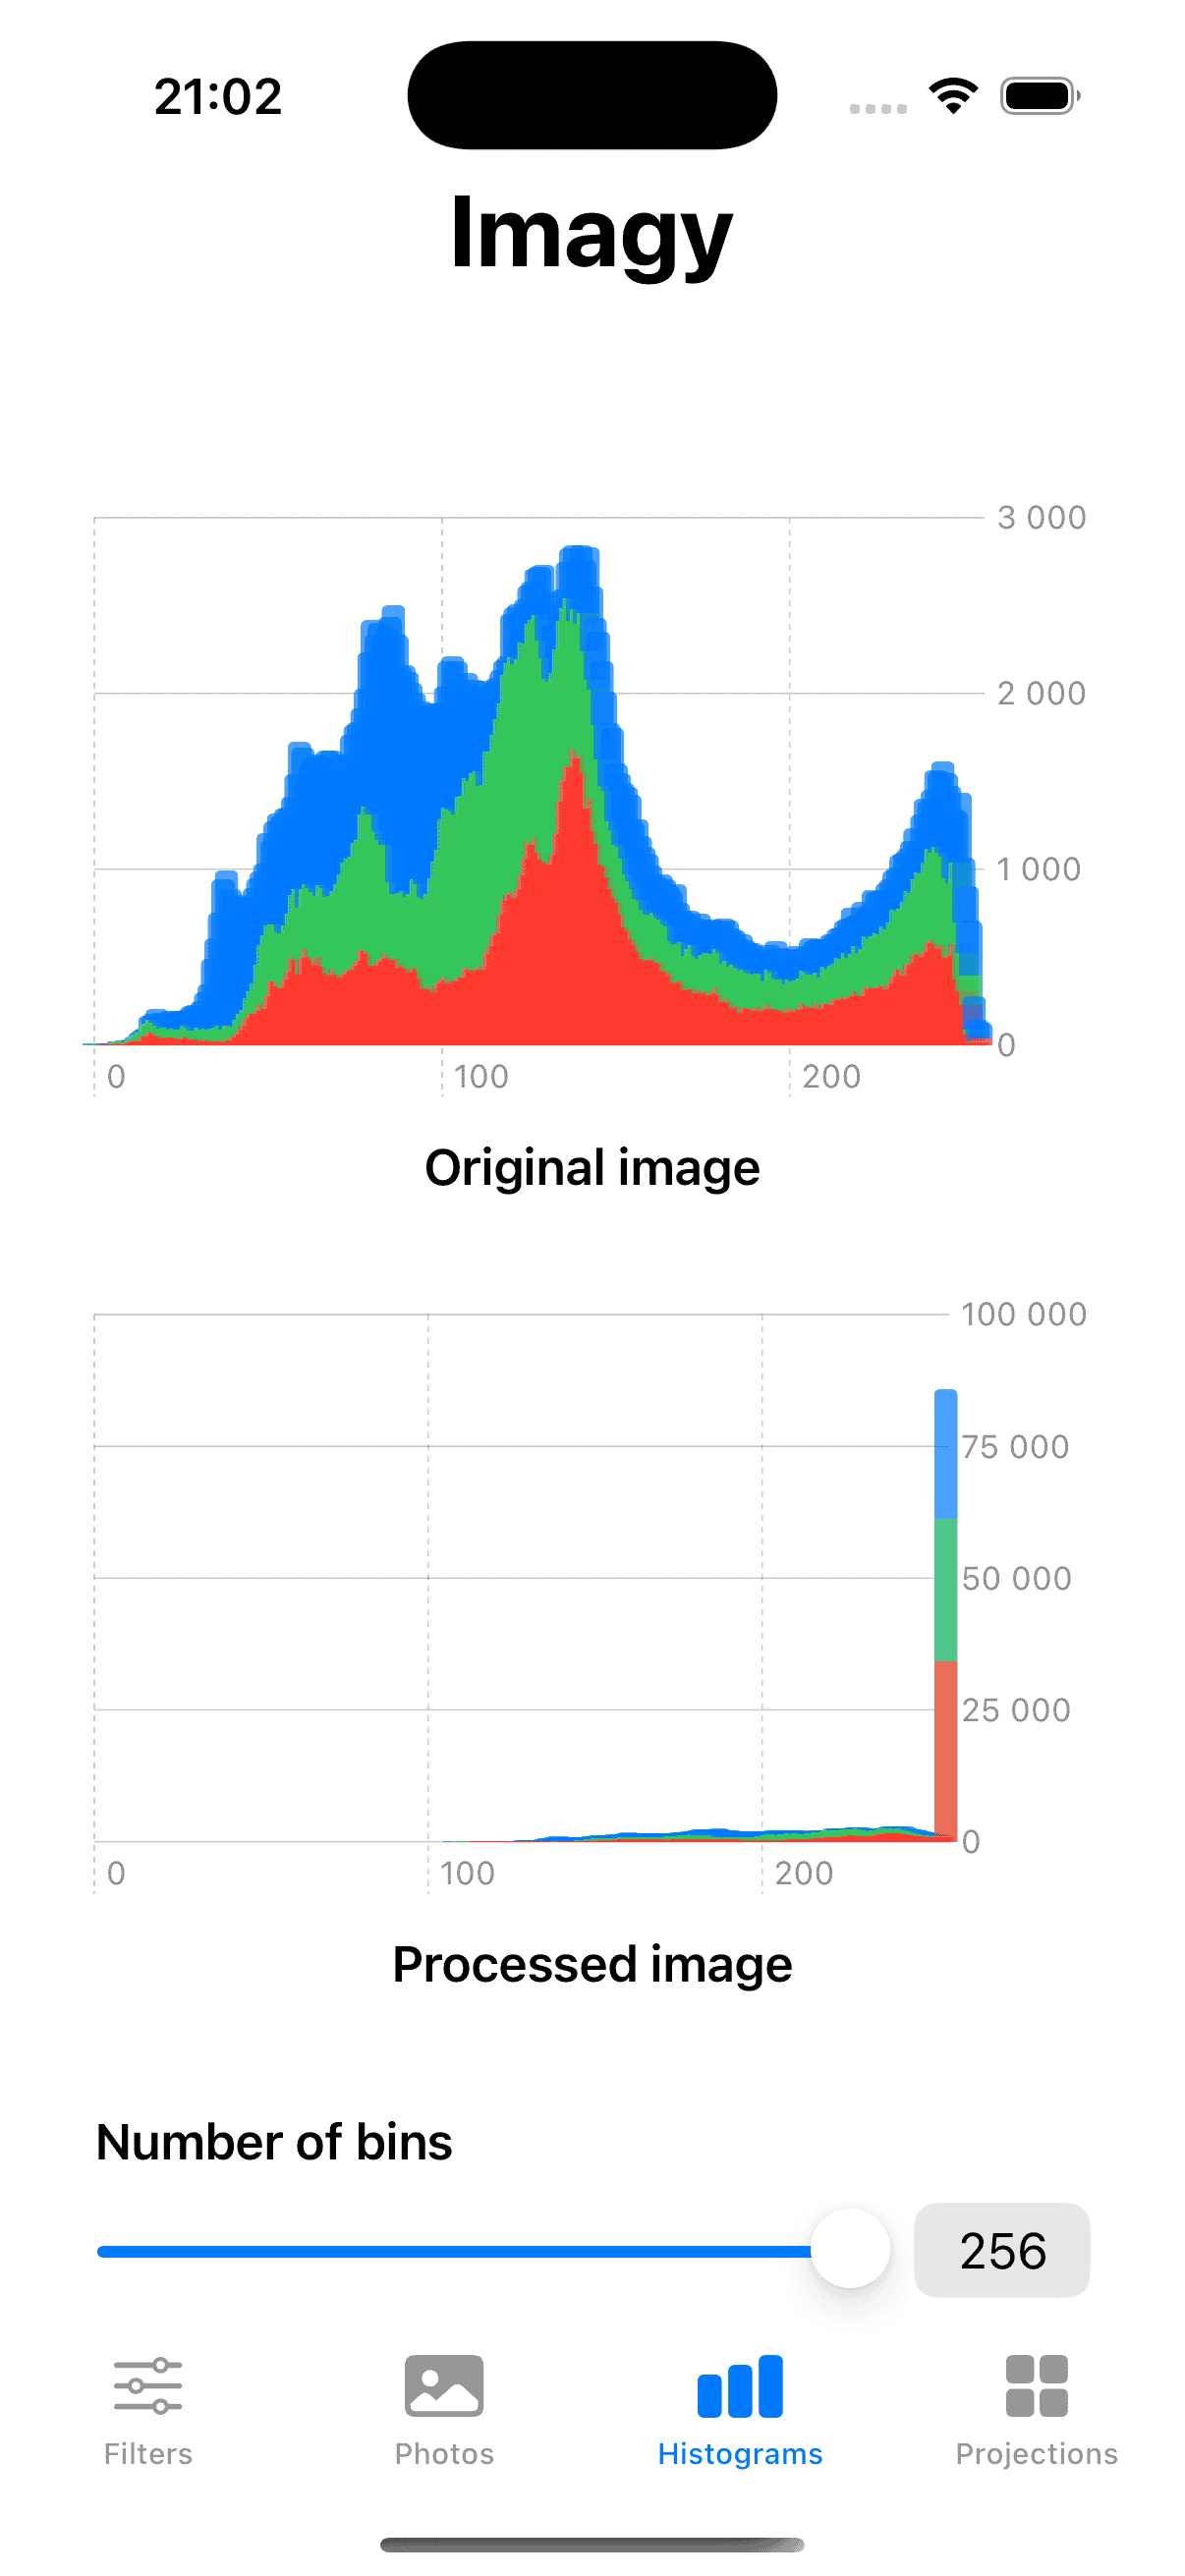
\includegraphics[width=0.25\linewidth]{images/dog_brightness_100_histogram.png}
    \caption{Histogram for dog's brightness filter with intensity=100.}
    \label{fig:dog_brightness_100_histogram}
\end{figure}

\subsection{Contrast}

\begin{itemize}
    \item \texttt{static var name: String = "Contrast"}
    \item \texttt{adjustment: Double} - defaultowo $1.2$, ograniczony do zakresu $0.0-2.0$, pobierany z widoku GUI ze stepem $0.1$. Każdy pikesel (kanały wszystkie prócz alfa) transformowany jest zgodnie z wzorem:\\
          $$
              UInt8(min(255, max(0, Int((Double(pixel) - 128) * adjustment + 128))))
          $$
    \item Filtr zwiększa / zmniejsza różnicę między jasnymi a ciemnymi obszarami obrazu, wynikowo dając obraz o bardziej wyrazistych, stonowanych kolorach.
    \item Filtr jest używany do poprawy jakości (czytelności w 'zlanych' obszarach), stylizacji obrazów (dramatyczny wygląd) czy poprawy ich czytelności.
\end{itemize}

\begin{figure}[H]
    \centering
    \begin{subfigure}{0.2\textwidth}
        \centering
        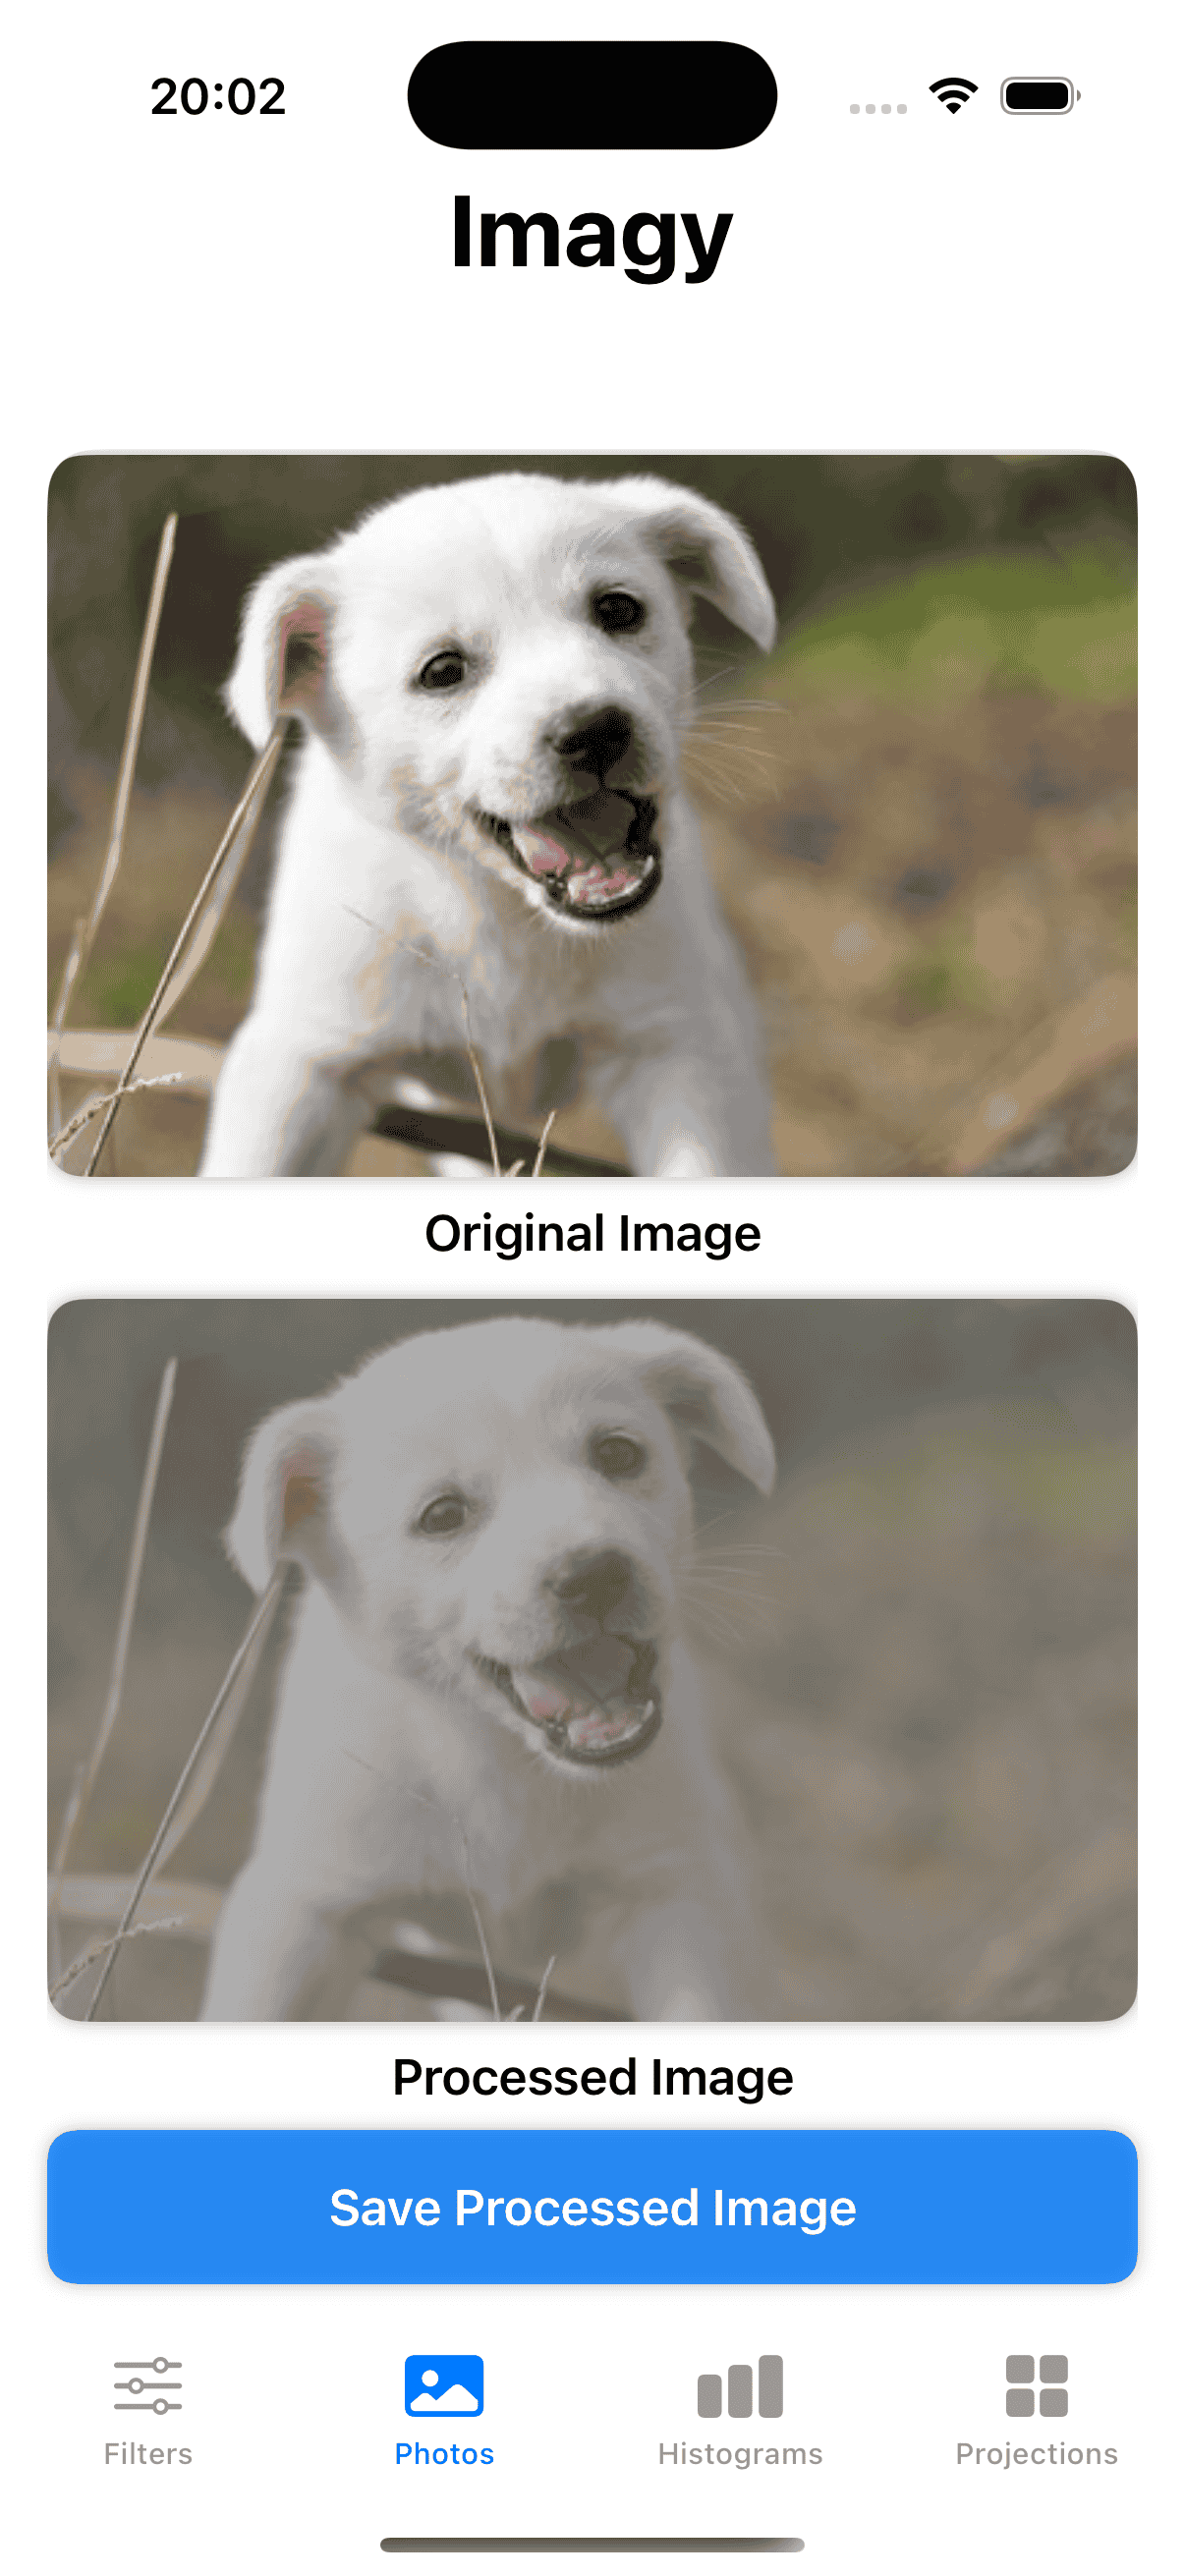
\includegraphics[width=\linewidth]{images/dog_contrast_0.4.png}
        \caption{adjustment=0.4}
        \label{fig:dog_contrast_0}
    \end{subfigure}
    \hfill
    \begin{subfigure}{0.2\textwidth}
        \centering
        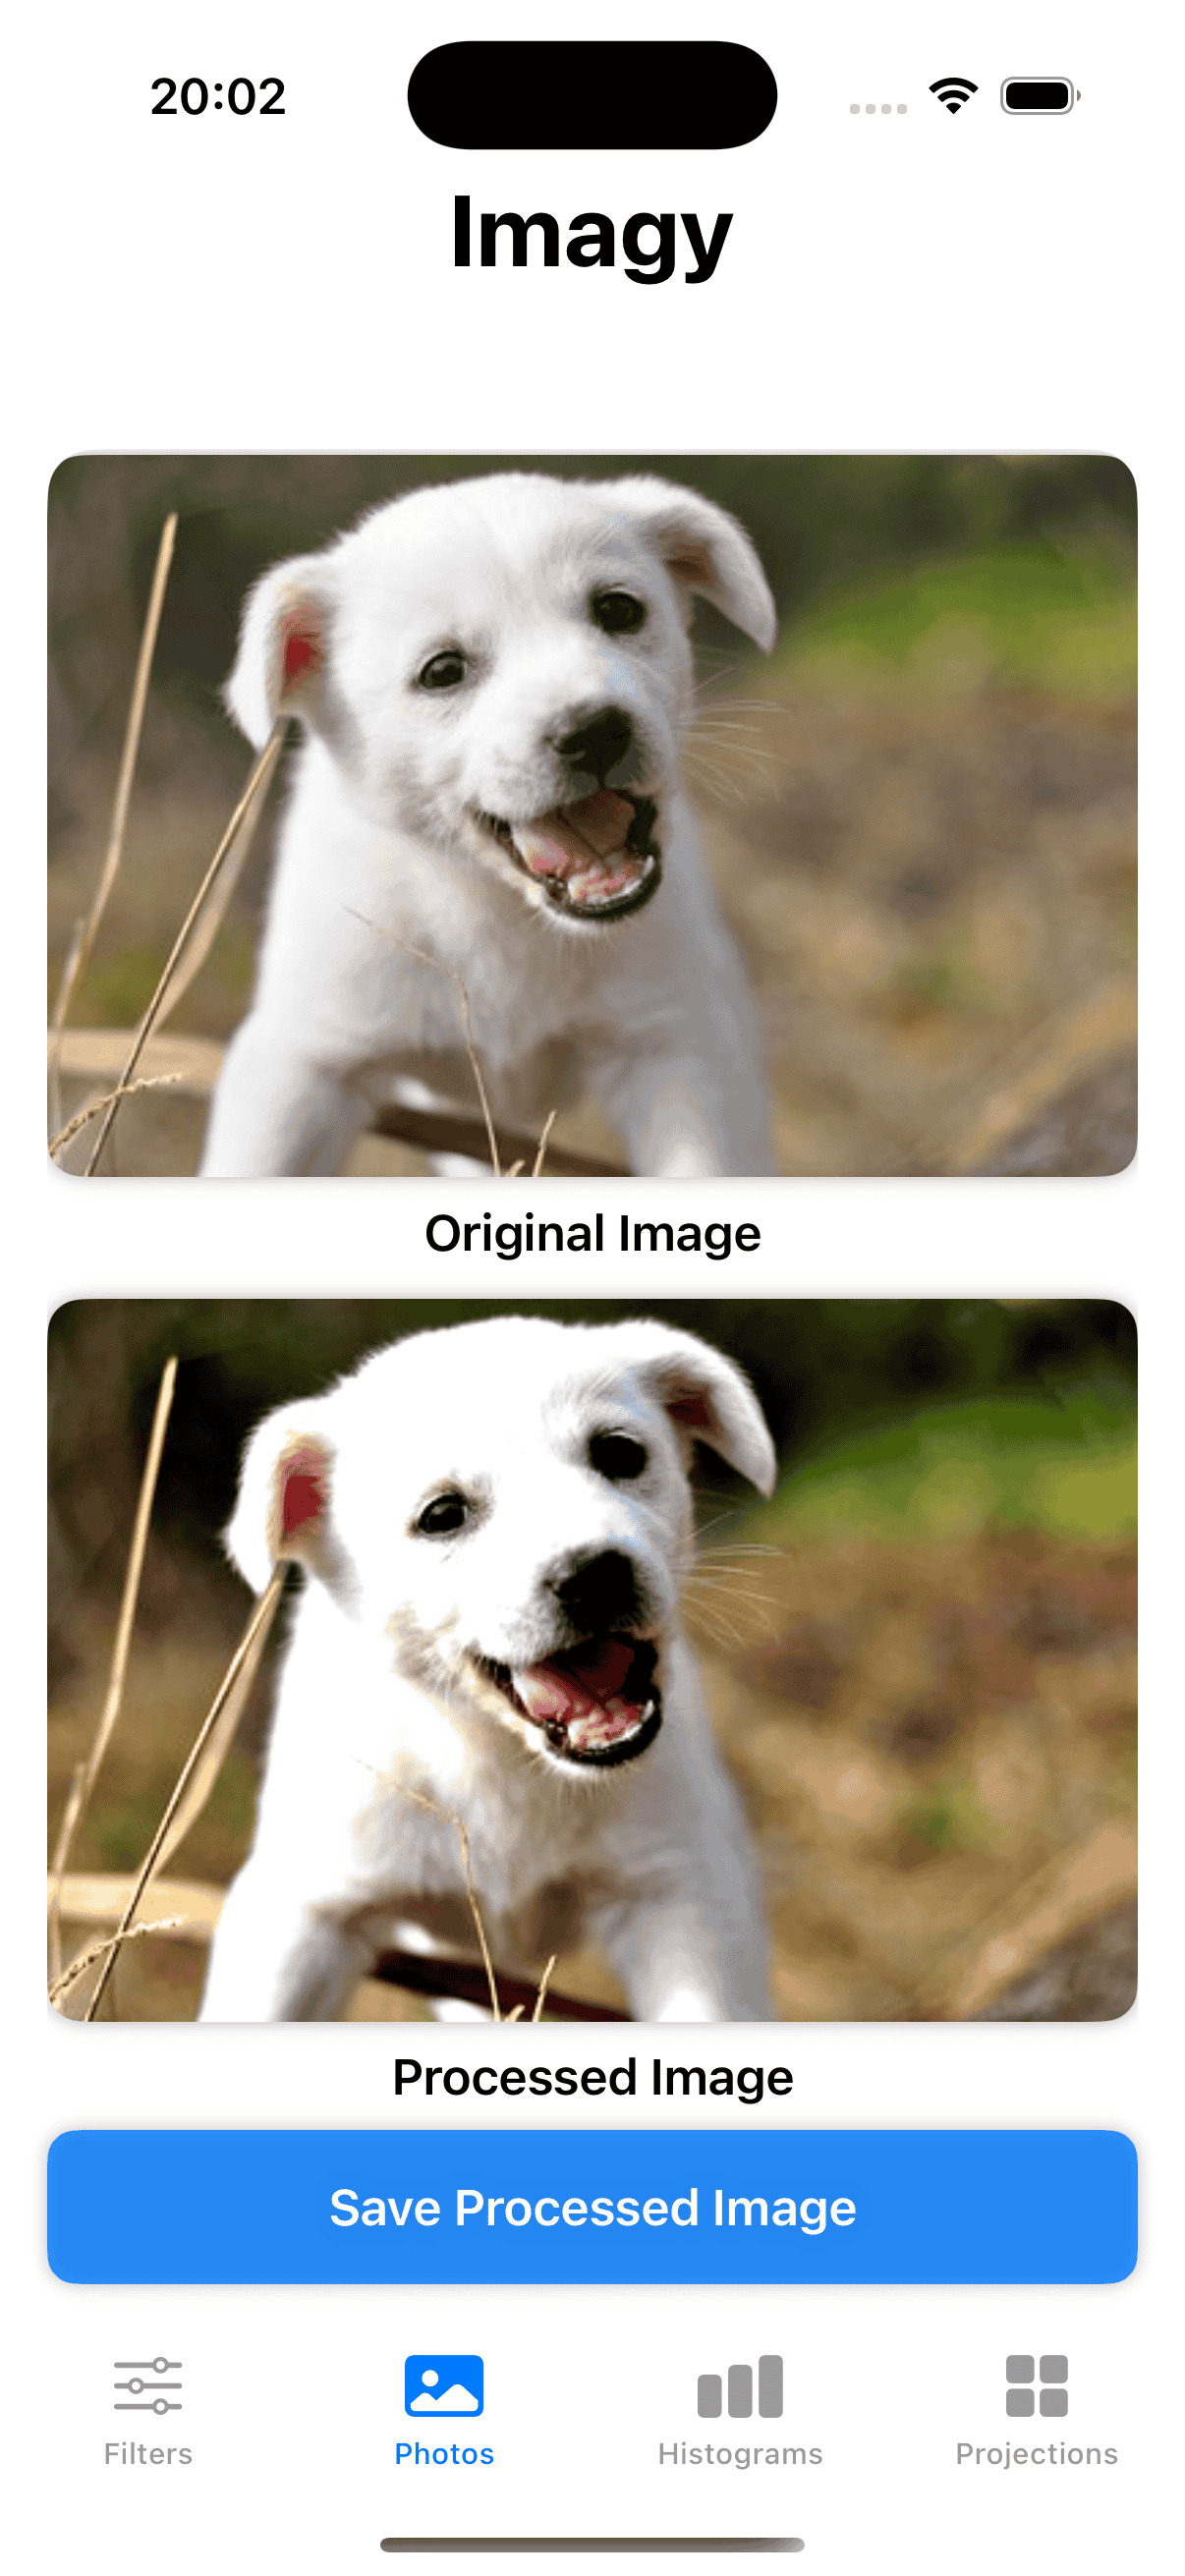
\includegraphics[width=\linewidth]{images/dog_contrast_1.6.png}
        \caption{adjustment=1.6}
        \label{fig:dog_contrast_1}
    \end{subfigure}
    \hfill
    \begin{subfigure}{0.2\textwidth}
        \centering
        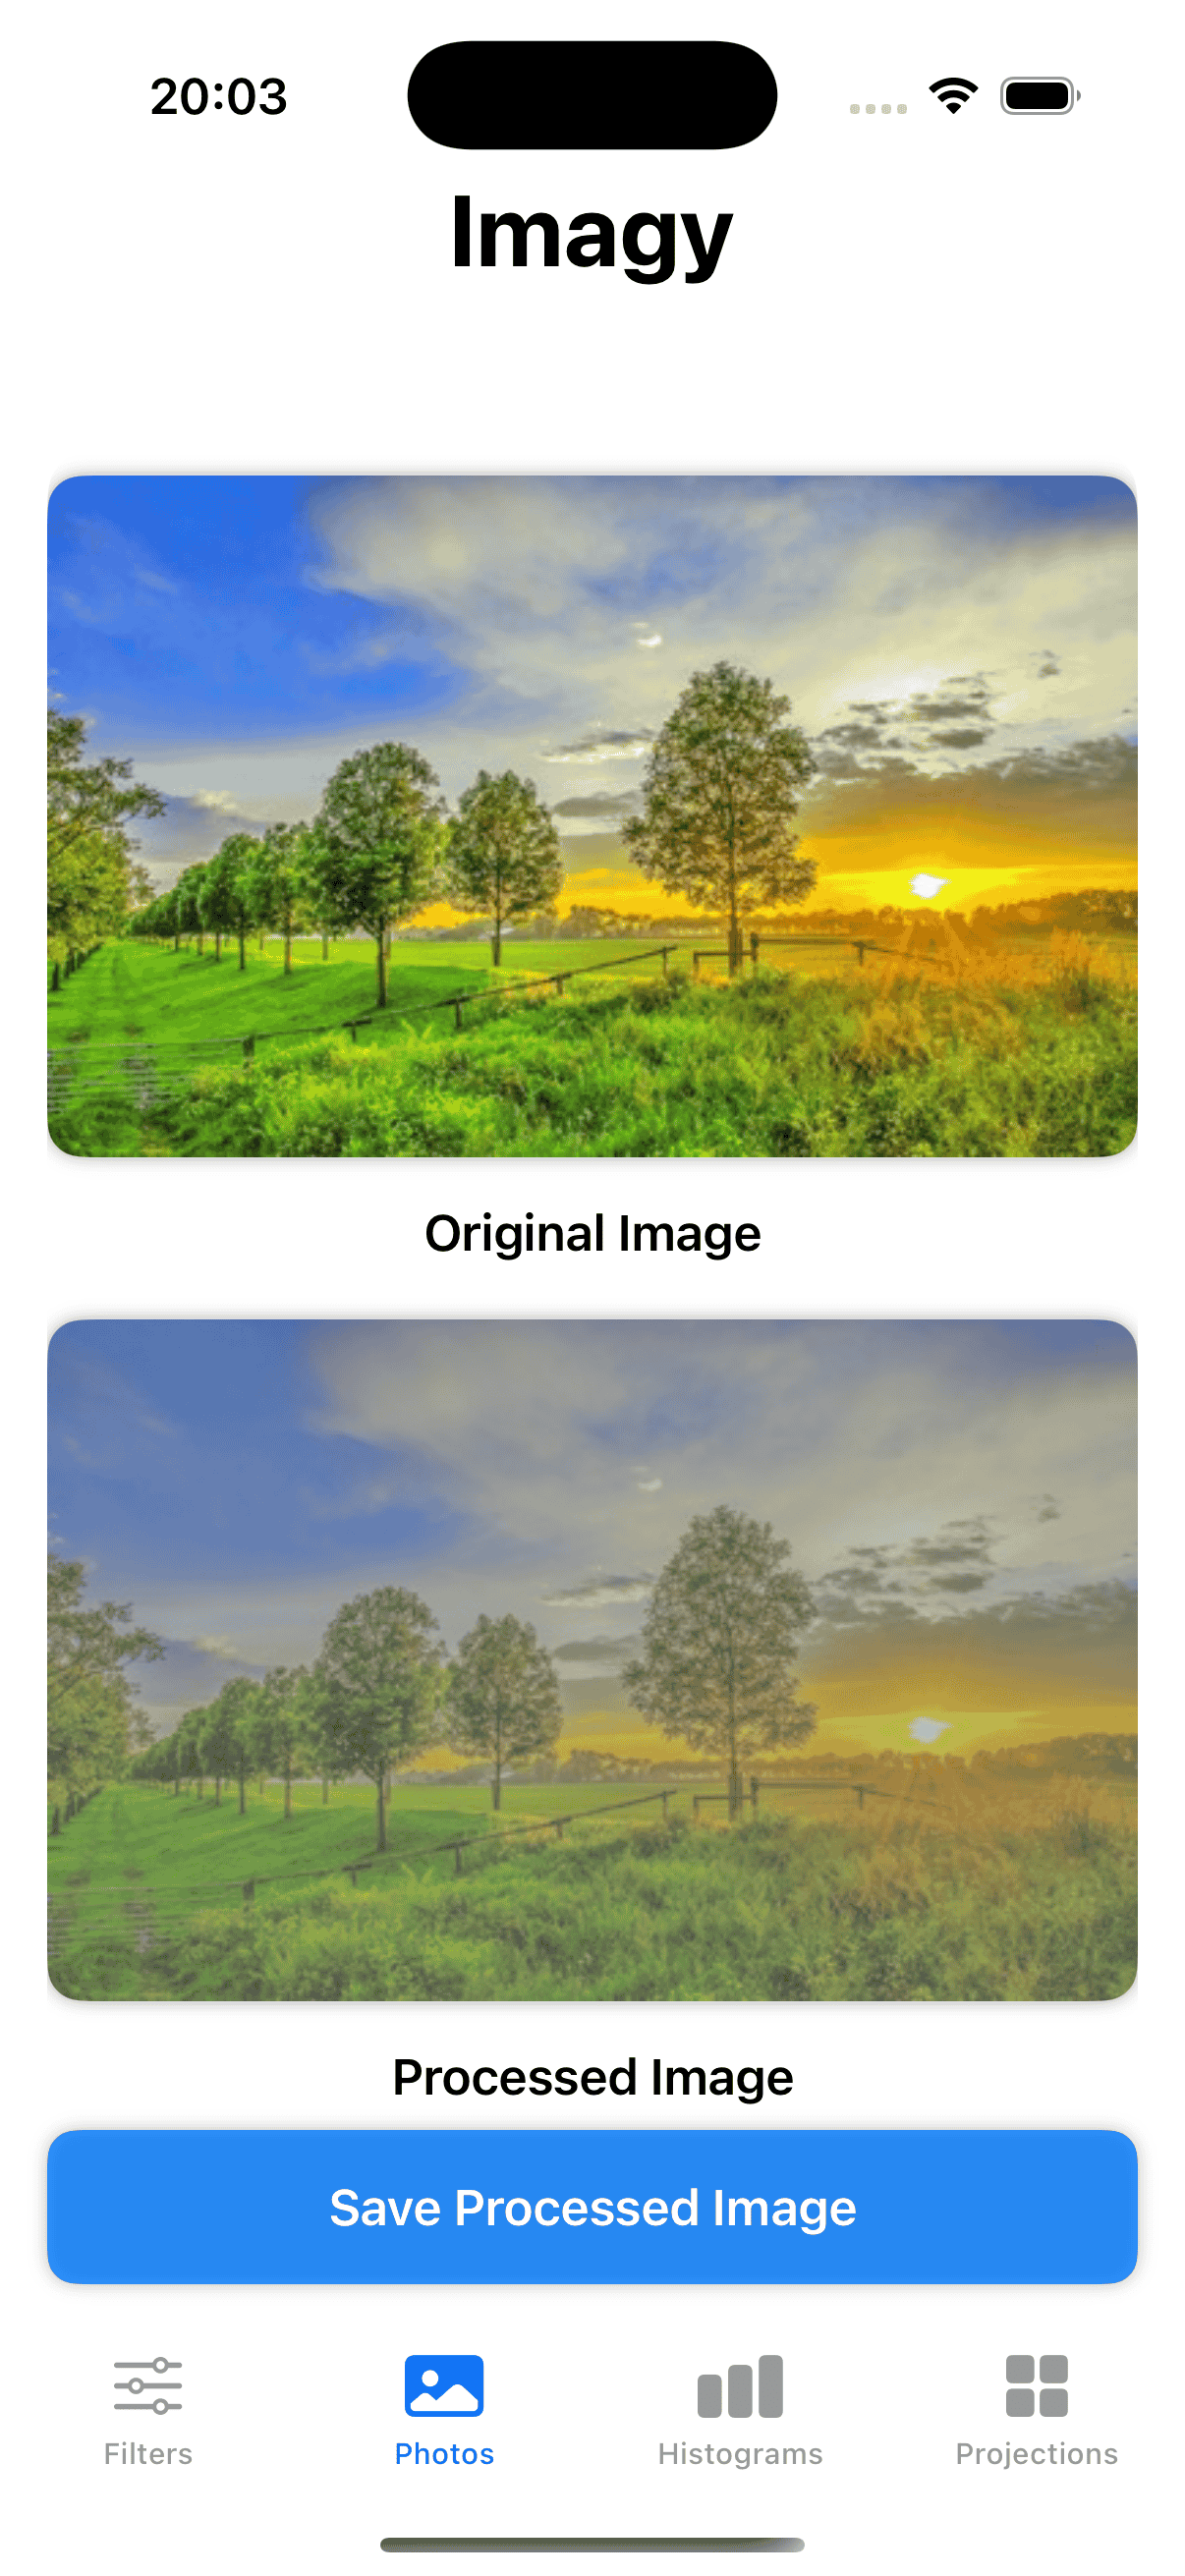
\includegraphics[width=\linewidth]{images/trees_contrast_0.4.png}
        \caption{adjustment=0.4}
        \label{fig:trees_contrast_0}
    \end{subfigure}
    \hfill
    \begin{subfigure}{0.2\textwidth}
        \centering
        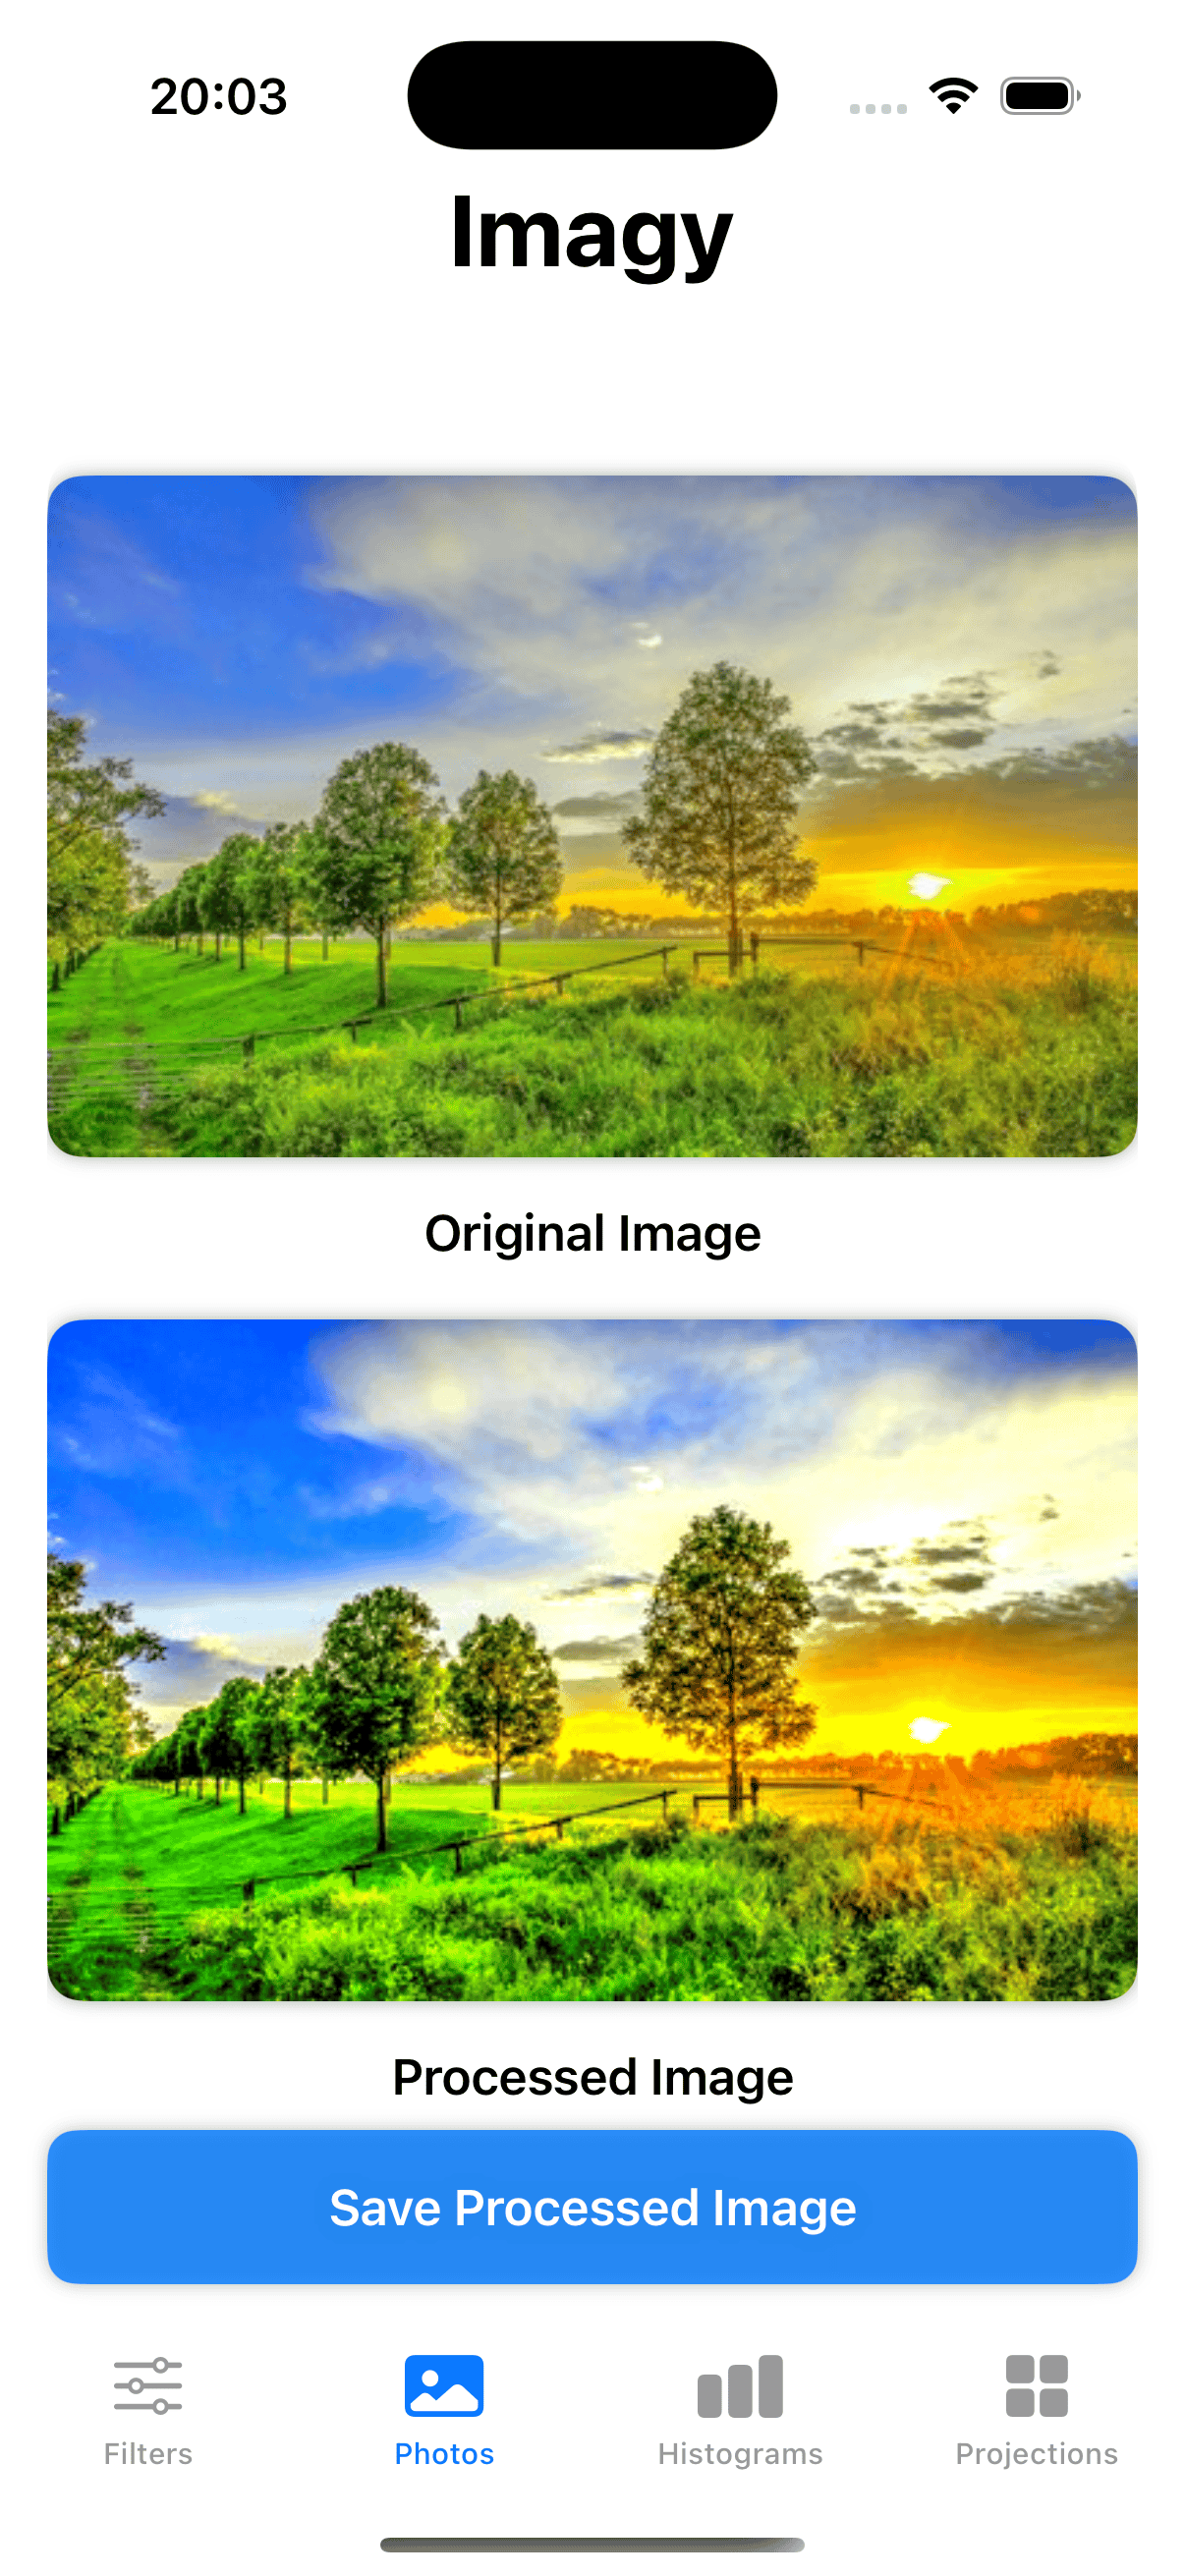
\includegraphics[width=\linewidth]{images/trees_contrast_1.6.png}
        \caption{adjustment=1.6}
        \label{fig:trees_contrast_1}
    \end{subfigure}
    \caption{Contrast filter - demonstracja. Mały adjustment prowadzi do zdjęć przykrytych szarością, podczas gdy większa wartość $1.6$ produkuje zdjęcia o wręcz nienaturalnie żywych kolorach.}
    \label{fig:contrast}
\end{figure}

\subsection{CustomKernel}

\begin{itemize}
    \item \texttt{static var name: String = "Custom Kernel"}
    \item \texttt{kernel: [[Float]]} - kernel konwolucji pobierany z GUI. Ze względów ograniczeń wielkości interfejsu na telefonach i czytelności, możliwe rozmiary to jedynie 3x3 bądź 5x5. Wartości w gui nie mają ograniczeń prócz wymuszonego typu danych Float.
\end{itemize}

\begin{figure}[H]
    \centering
    \begin{subfigure}{0.2\textwidth}
        \centering
        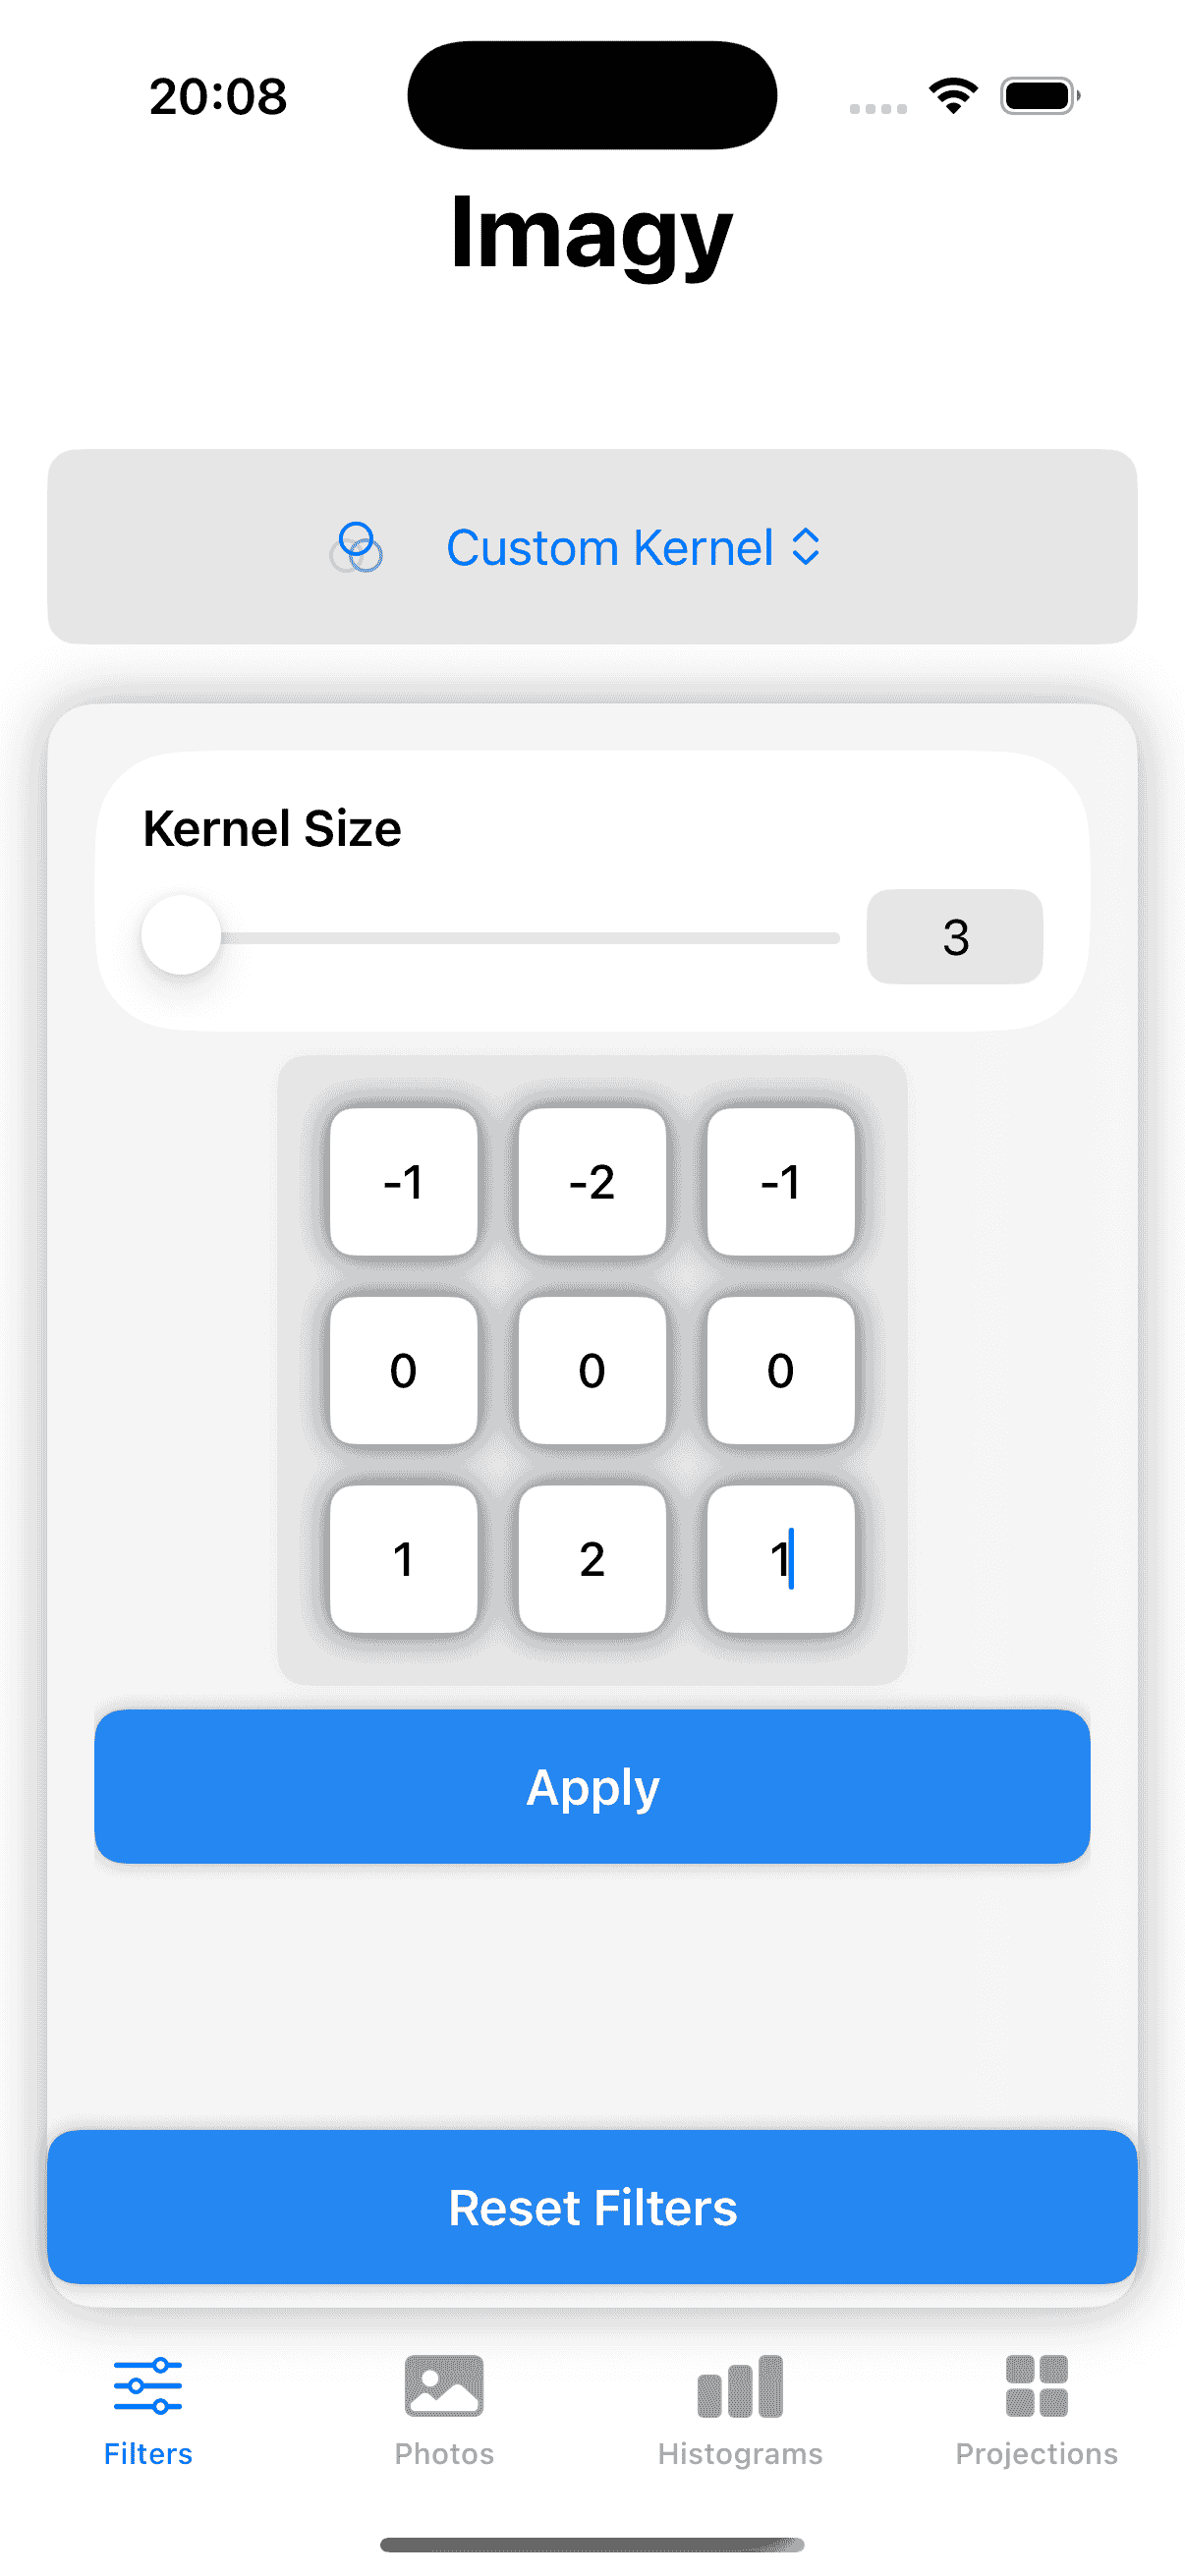
\includegraphics[width=\linewidth]{images/custom_vertical.png}
        \label{fig:custom_vertical}
    \end{subfigure}
    \hfill
    \begin{subfigure}{0.2\textwidth}
        \centering
        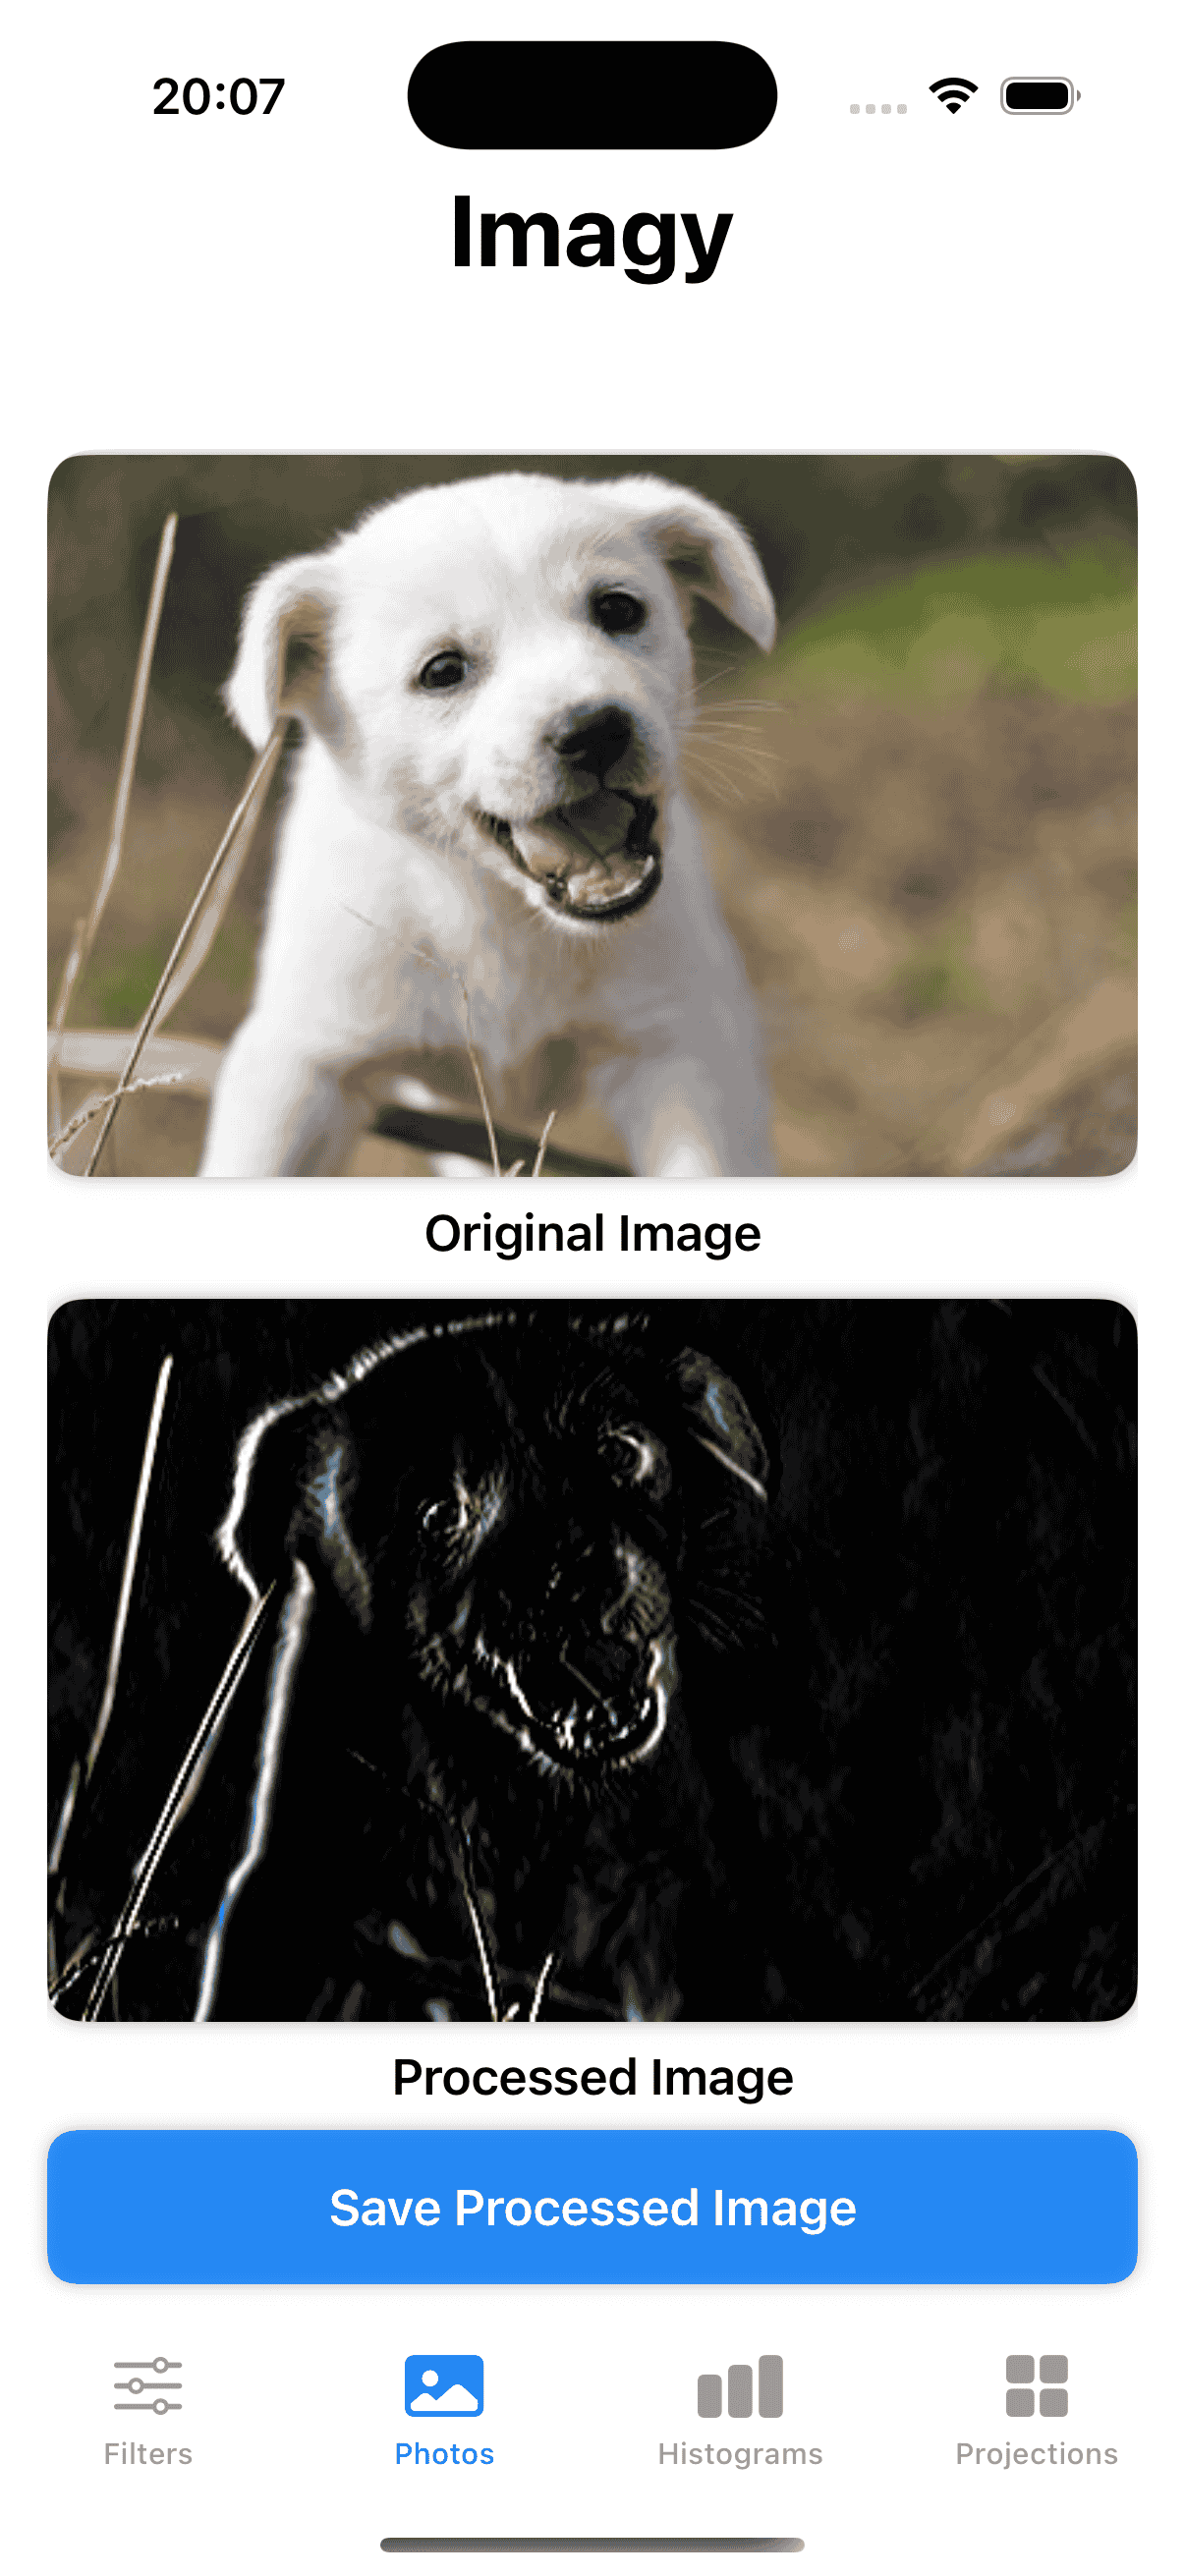
\includegraphics[width=\linewidth]{images/dog_custom_vertical.png}
        \label{fig:dog_custom_vertical}
    \end{subfigure}
    \hfill
    \begin{subfigure}{0.2\textwidth}
        \centering
        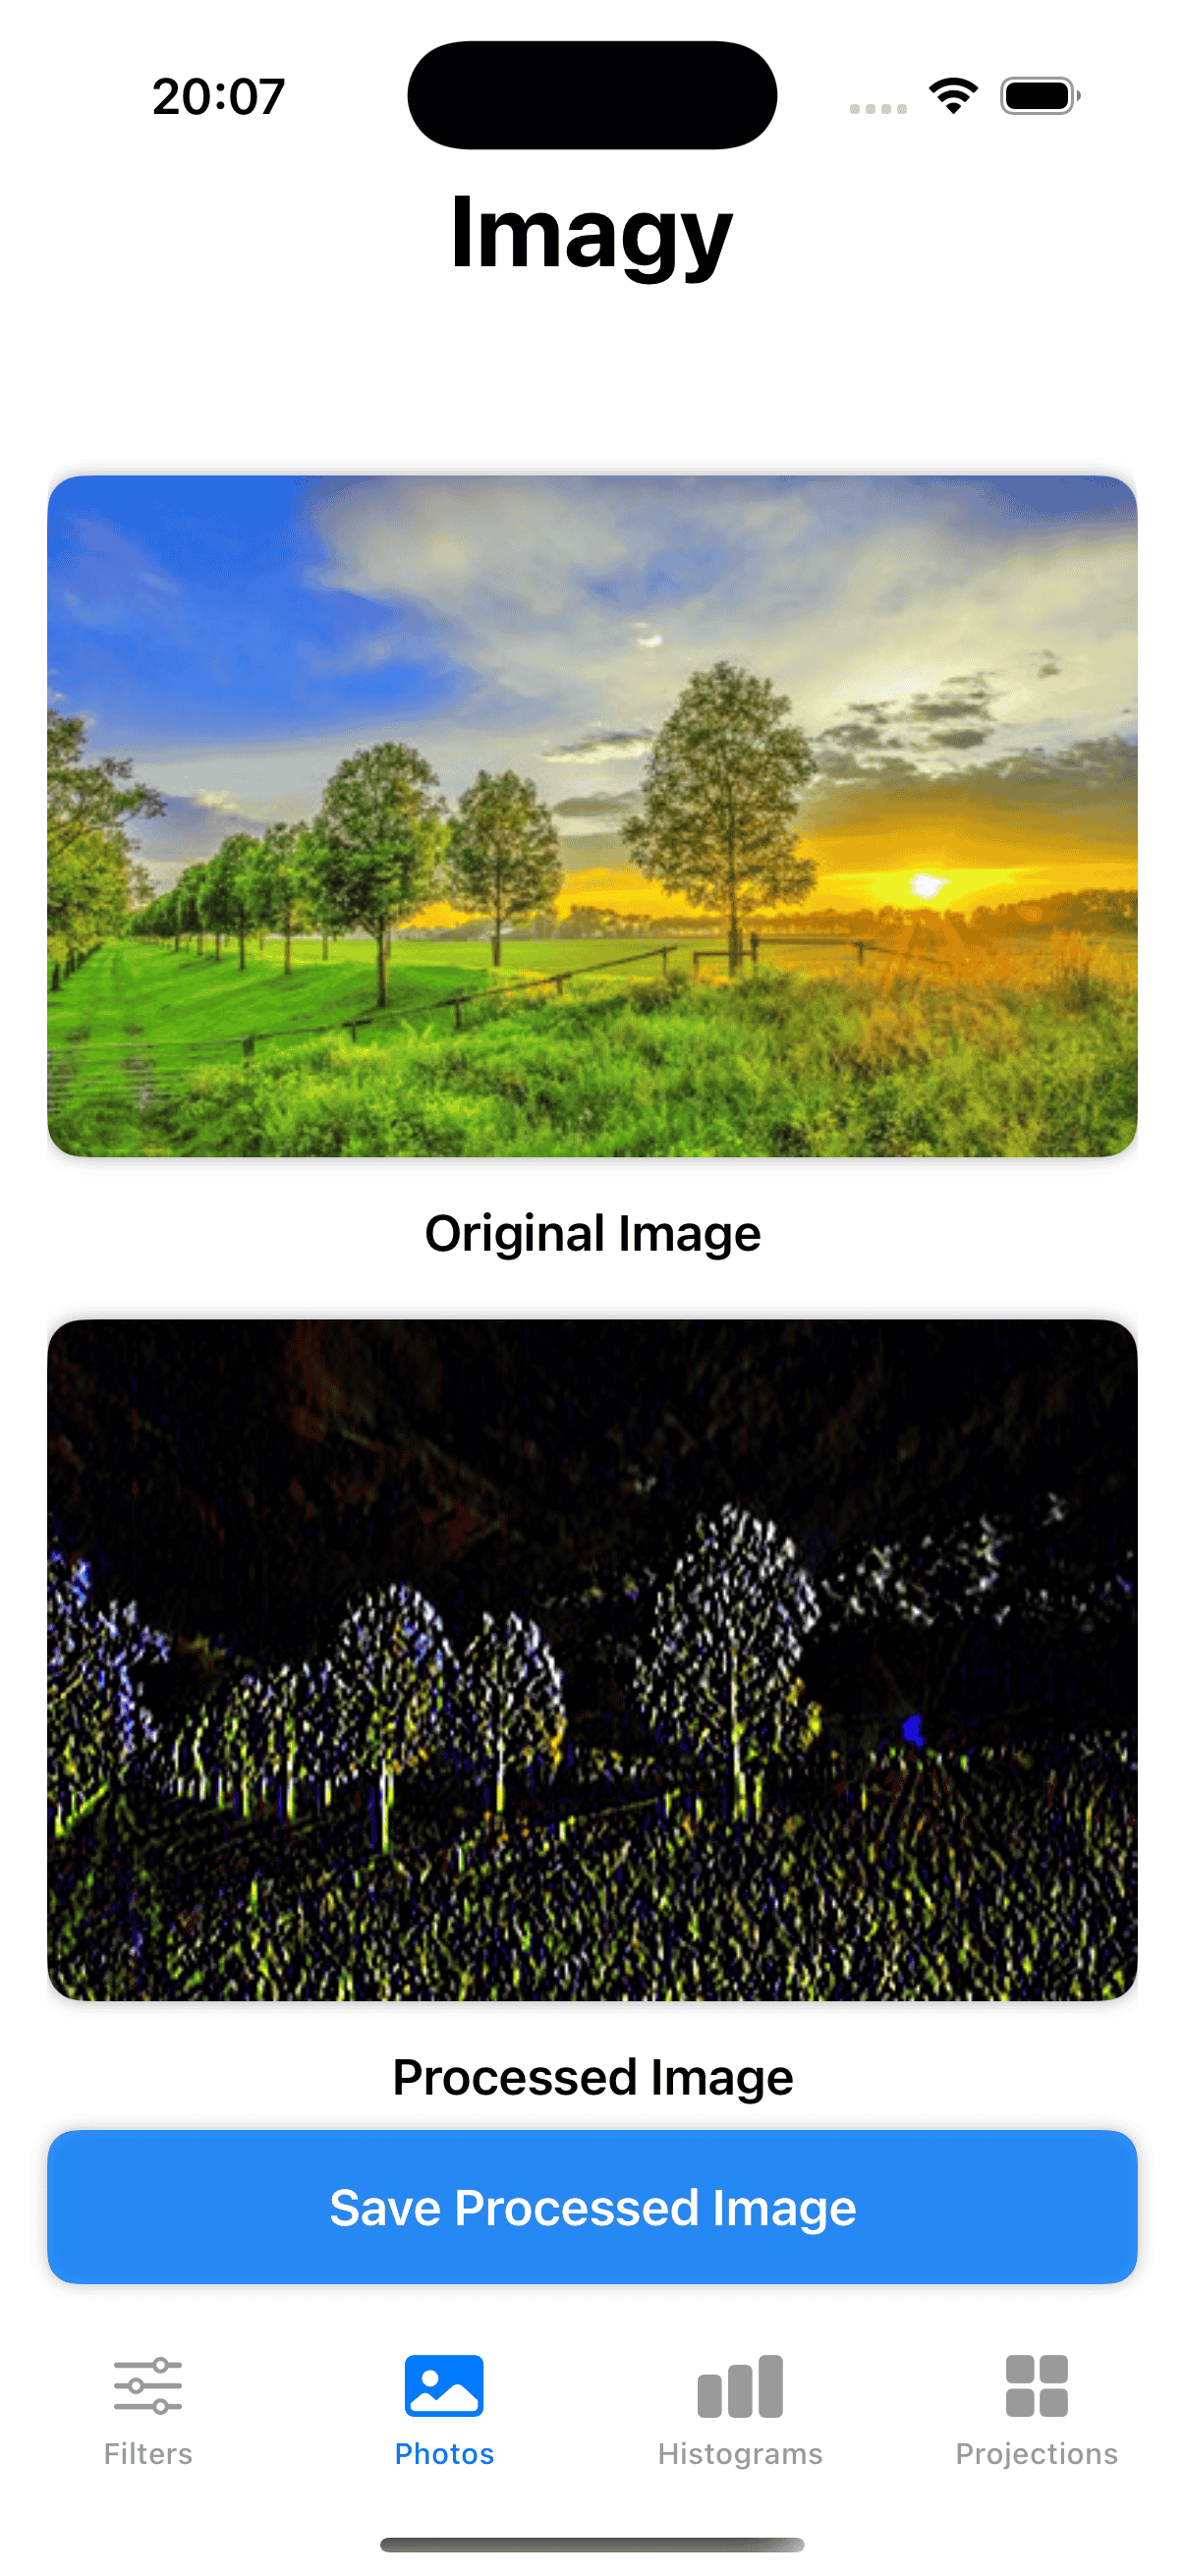
\includegraphics[width=\linewidth]{images/trees_custom_vertical.png}
        \label{fig:trees_custom_vertical}
    \end{subfigure}
    \caption{Custom kernel filter - demonstracja. Tutaj lewe zdjęcie pokazuje zastosowany kernel transformacji - Sobel vertival. Na prawo wyniki.}
    \label{fig:custom_vertical}
\end{figure}

\begin{figure}[H]
    \centering
    \begin{subfigure}{0.2\textwidth}
        \centering
        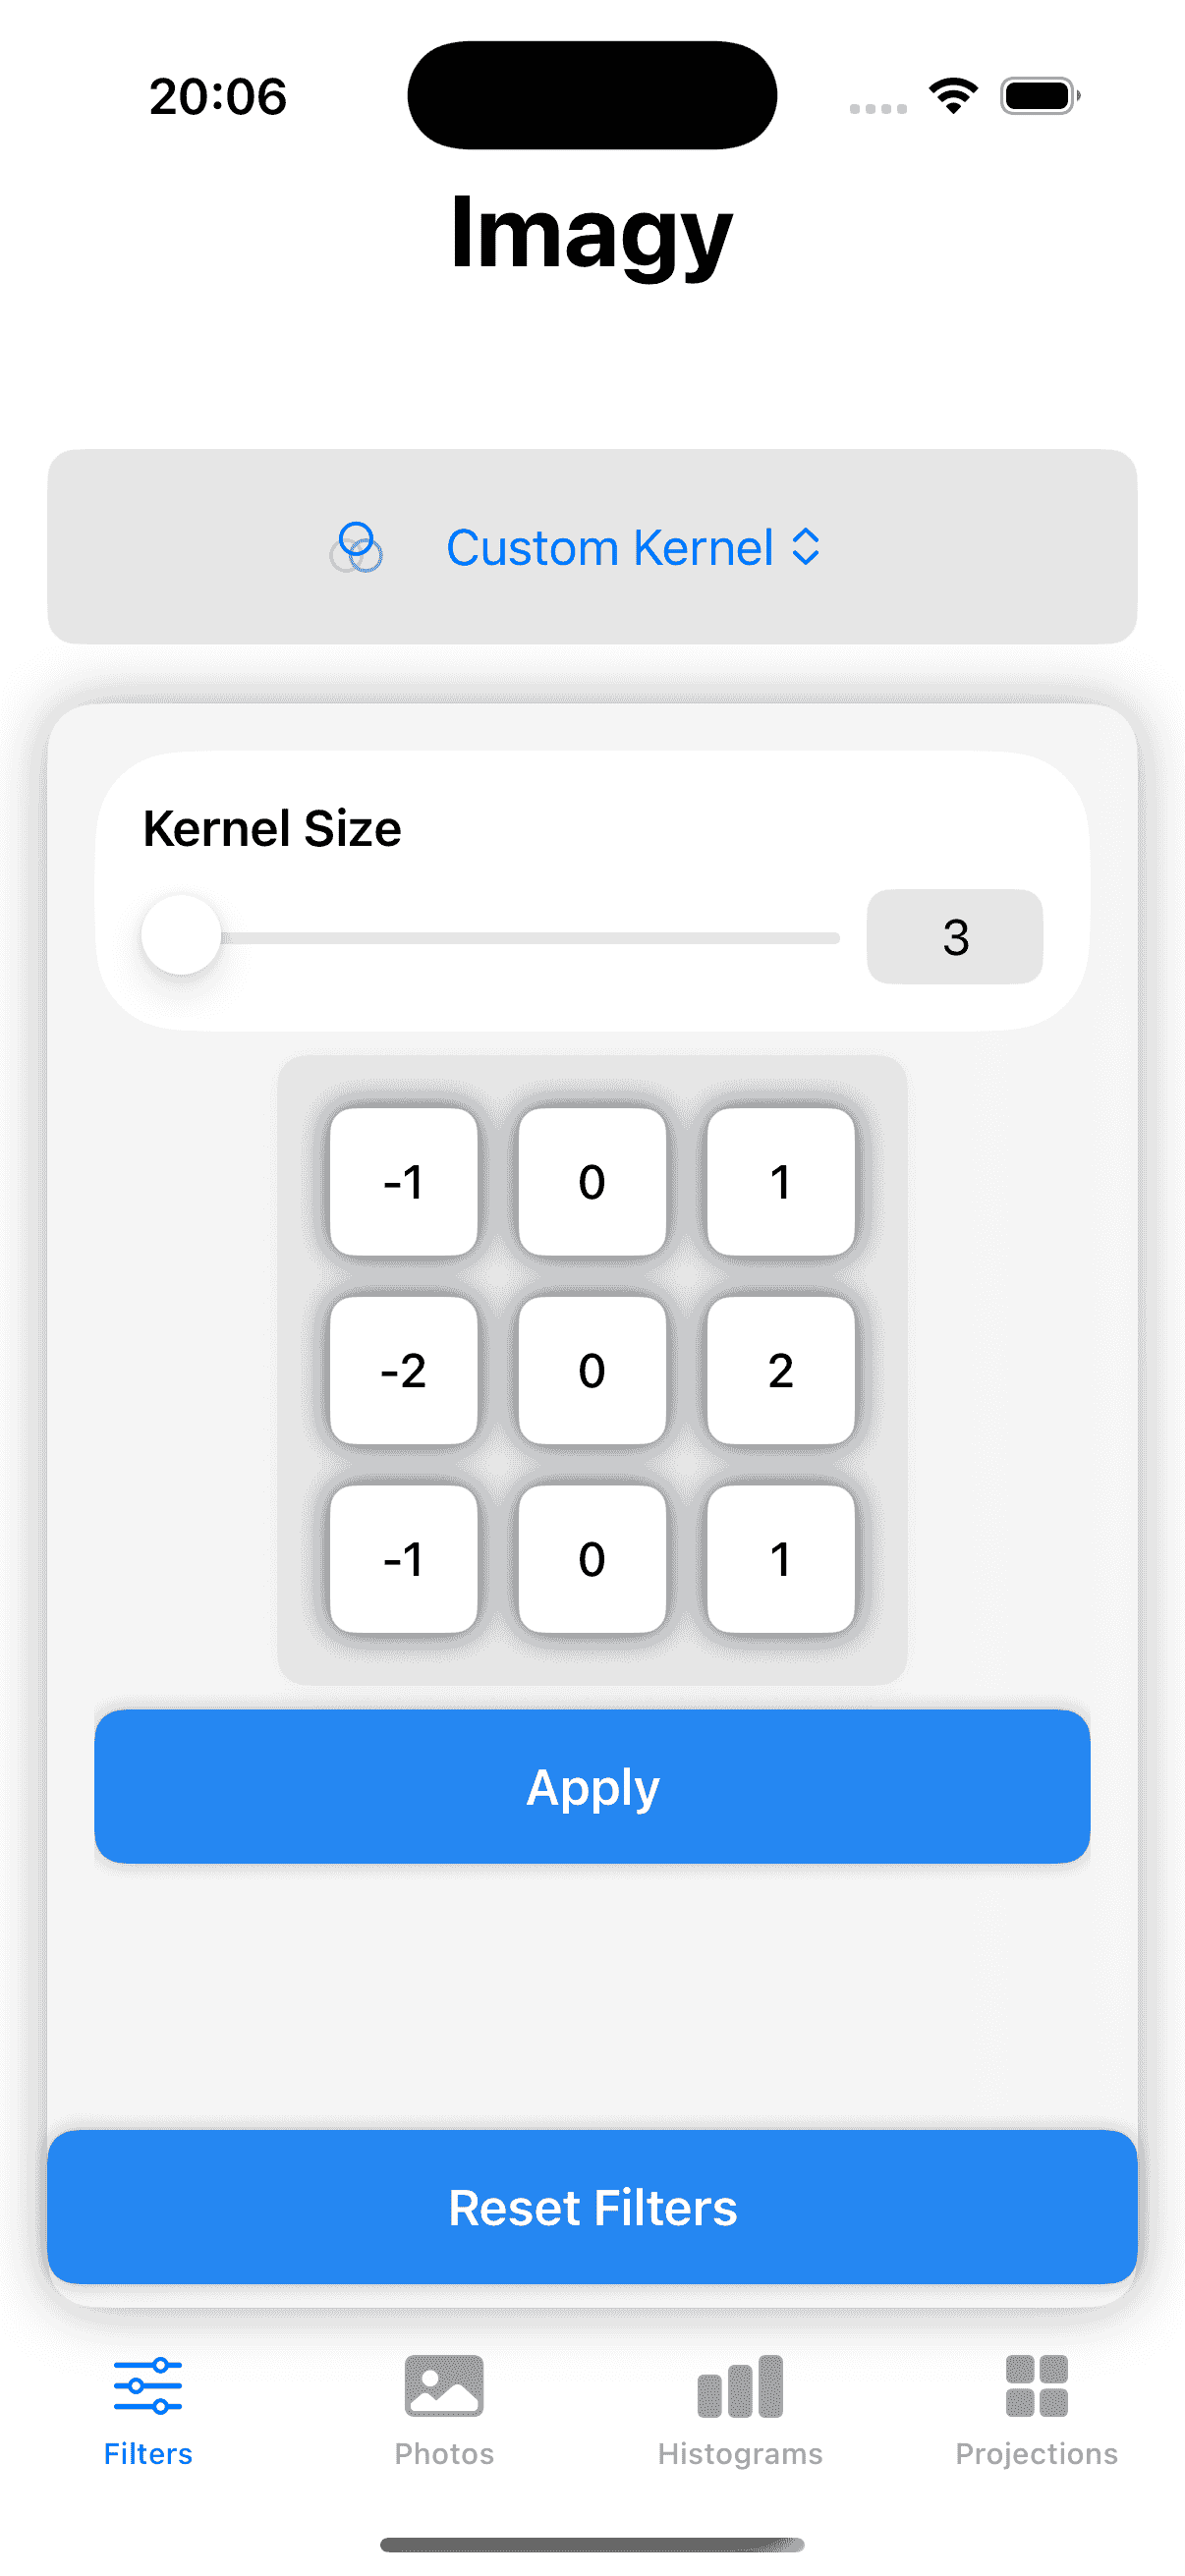
\includegraphics[width=\linewidth]{images/custom_horizontal.png}
        \label{fig:custom_horizontal}
    \end{subfigure}
    \hfill
    \begin{subfigure}{0.2\textwidth}
        \centering
        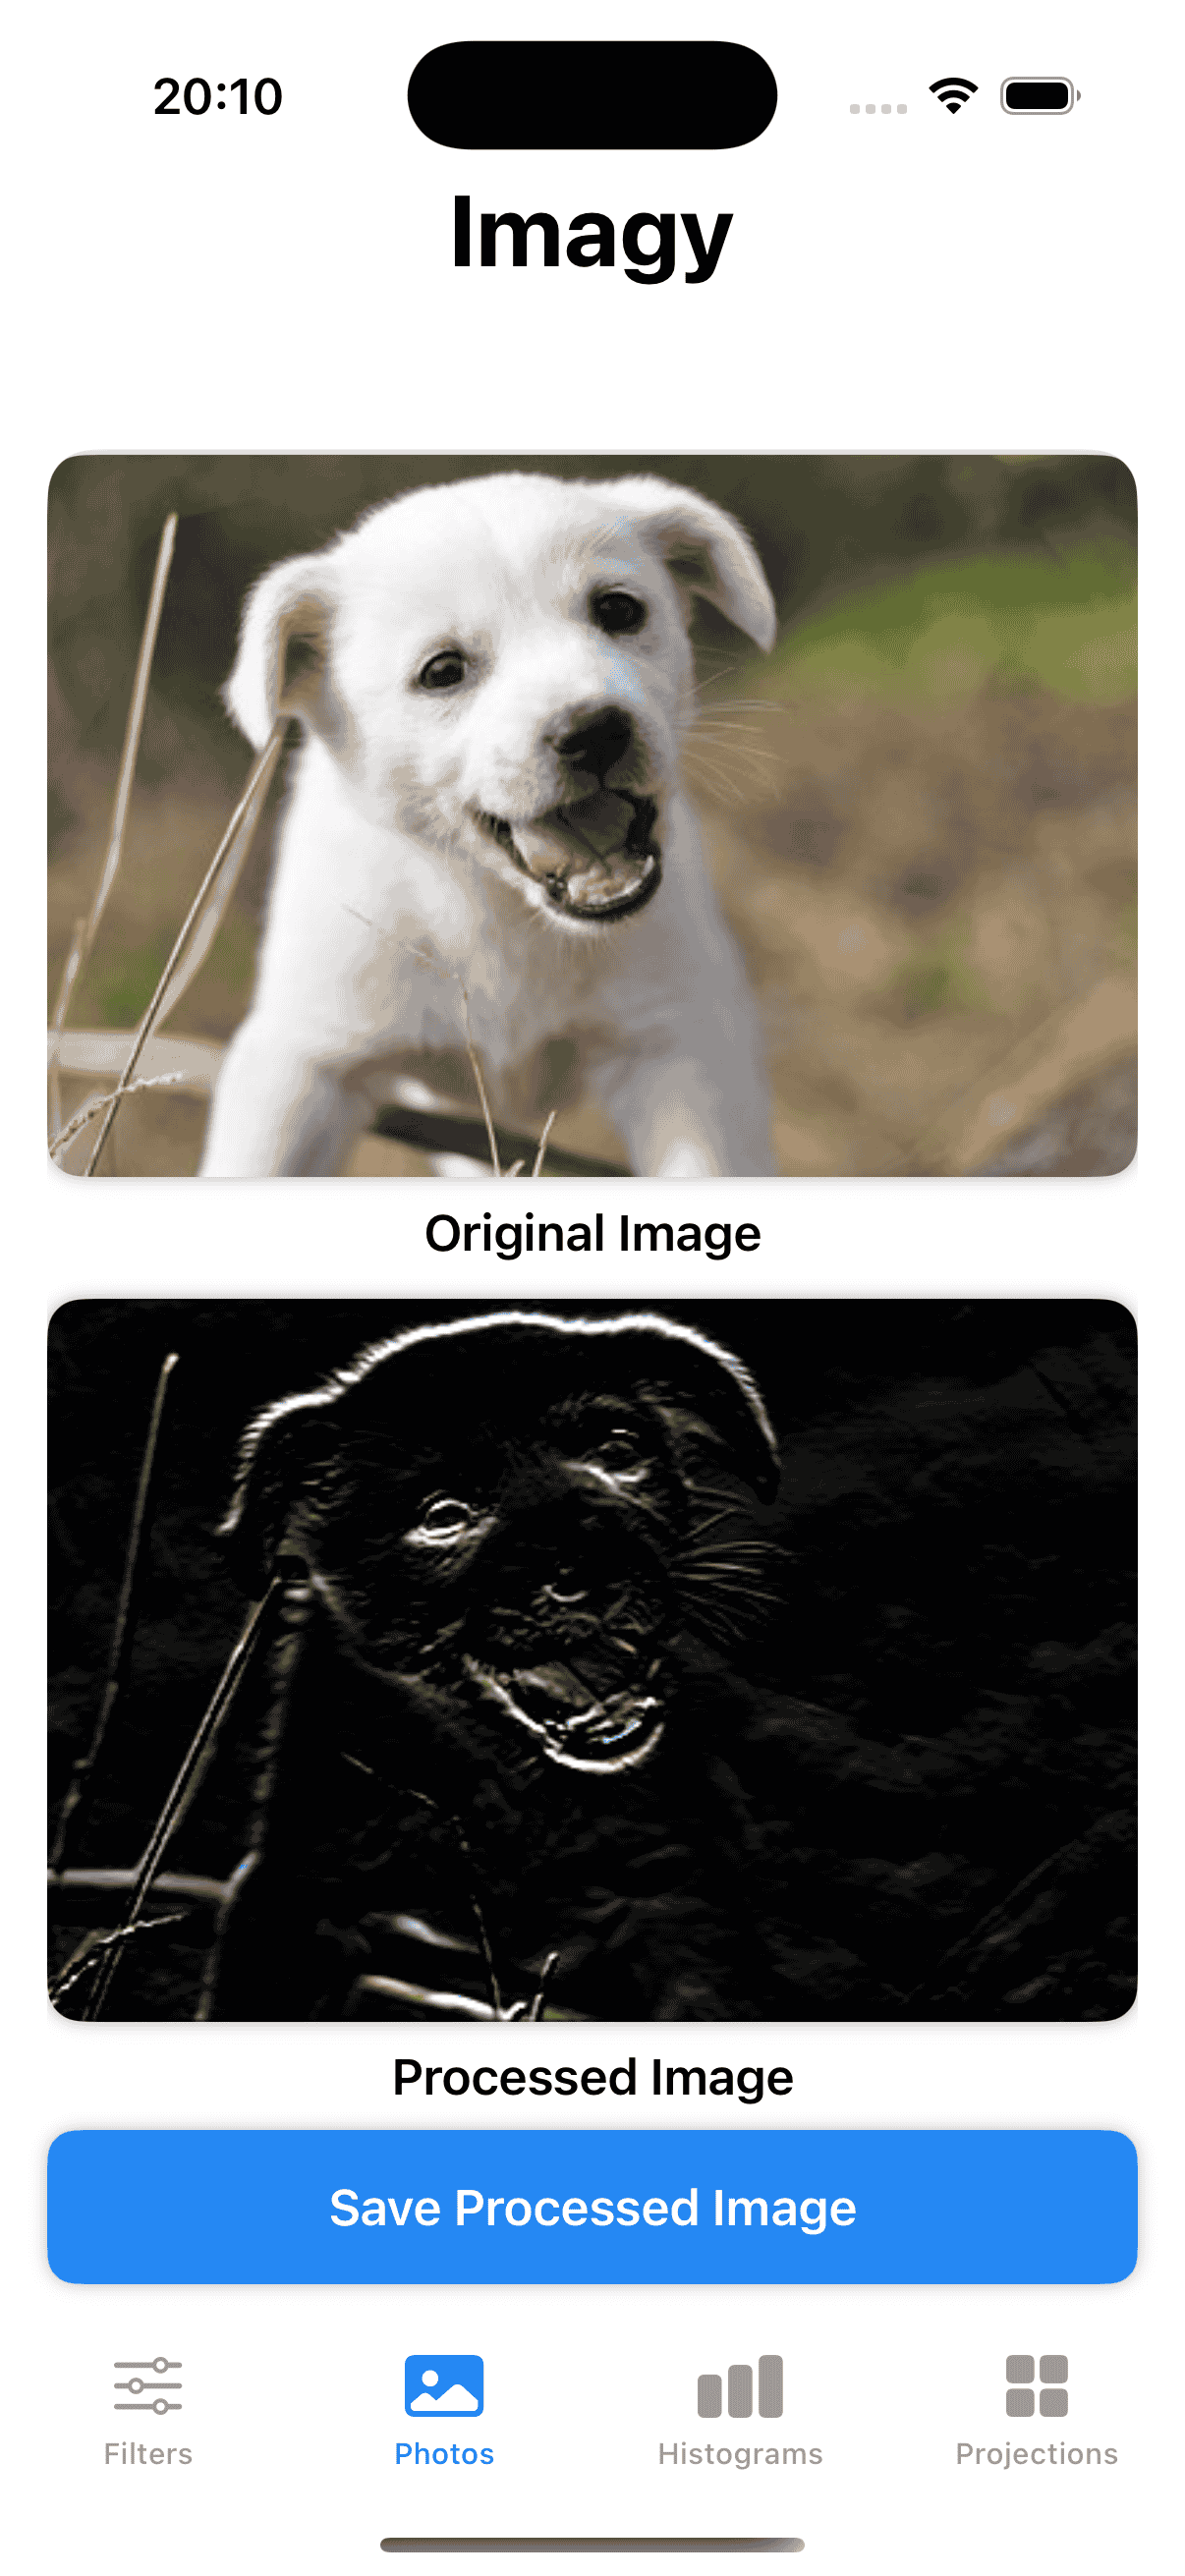
\includegraphics[width=\linewidth]{images/dog_custom_horizontal.png}
        \label{fig:dog_custom_horizontal}
    \end{subfigure}
    \hfill
    \begin{subfigure}{0.2\textwidth}
        \centering
        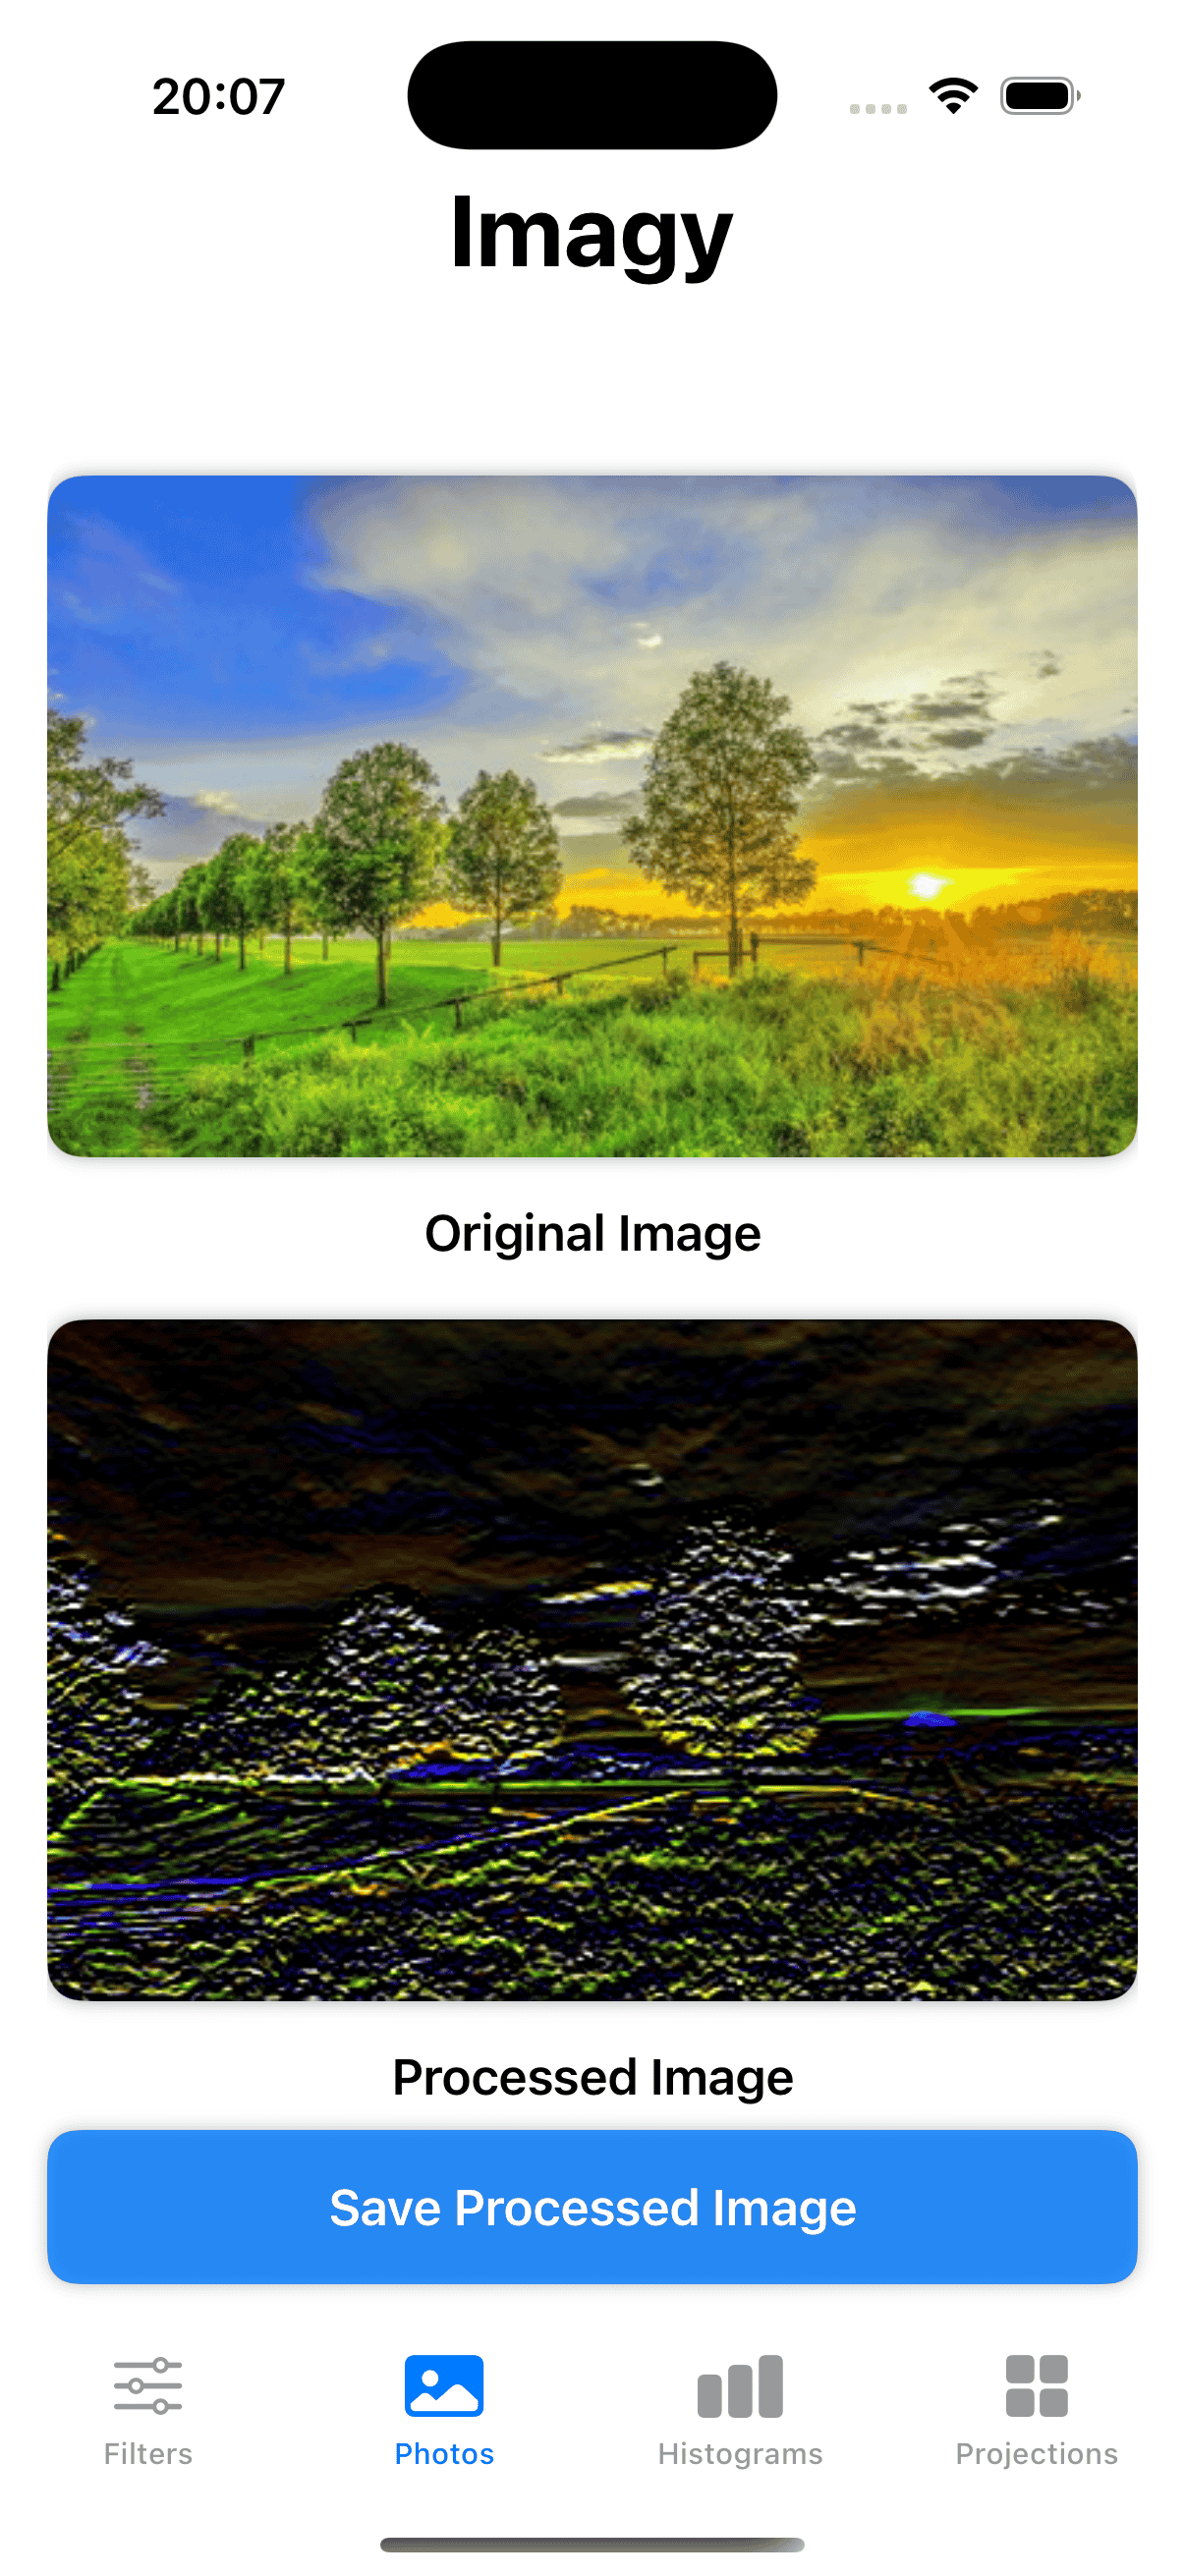
\includegraphics[width=\linewidth]{images/trees_custom_horizontal.png}
        \label{fig:trees_custom_horizontal}
    \end{subfigure}
    \caption{Custom kernel filter - demonstracja. Tutaj lewe zdjęcie pokazuje zastosowany kernel transformacji - Sobel vertival. Na prawo wyniki.}
    \label{fig:custom_horizontal}
\end{figure}

\subsection{Emboss}

\begin{itemize}
    \item \texttt{static var name: String = "Emboss"}
    \item \texttt{kernelType: EmbossKernelType} - 3 opcje na kernele konwolucji:
          \begin{itemize}
              \item default
                    \[
                        \begin{bmatrix}
                            -2 & -1 & 0 \\
                            -1 & 1  & 1 \\
                            0  & 1  & 2
                        \end{bmatrix}
                    \]
              \item strong
                    \[
                        \begin{bmatrix}
                            -1 & -1 & 0 \\
                            -1 & 1  & 1 \\
                            0  & 1  & 1
                        \end{bmatrix}
                    \]
              \item soft
                    \[
                        \begin{bmatrix}
                            -1   & -0.5 & 0   \\
                            -0.5 & 1    & 0.5 \\
                            0    & 0.5  & 1
                        \end{bmatrix}
                    \]
          \end{itemize}
    \item Filtr ten służy do nadawania obrazom efektu trójwymiarowości przez uwypulkanie krawędzi, tworząc efekt światła i cienia. Używany do podkreślania krawędzi i tworzenia tekstur.
\end{itemize}

\begin{figure}[H]
    \centering
    \begin{subfigure}{0.2\textwidth}
        \centering
        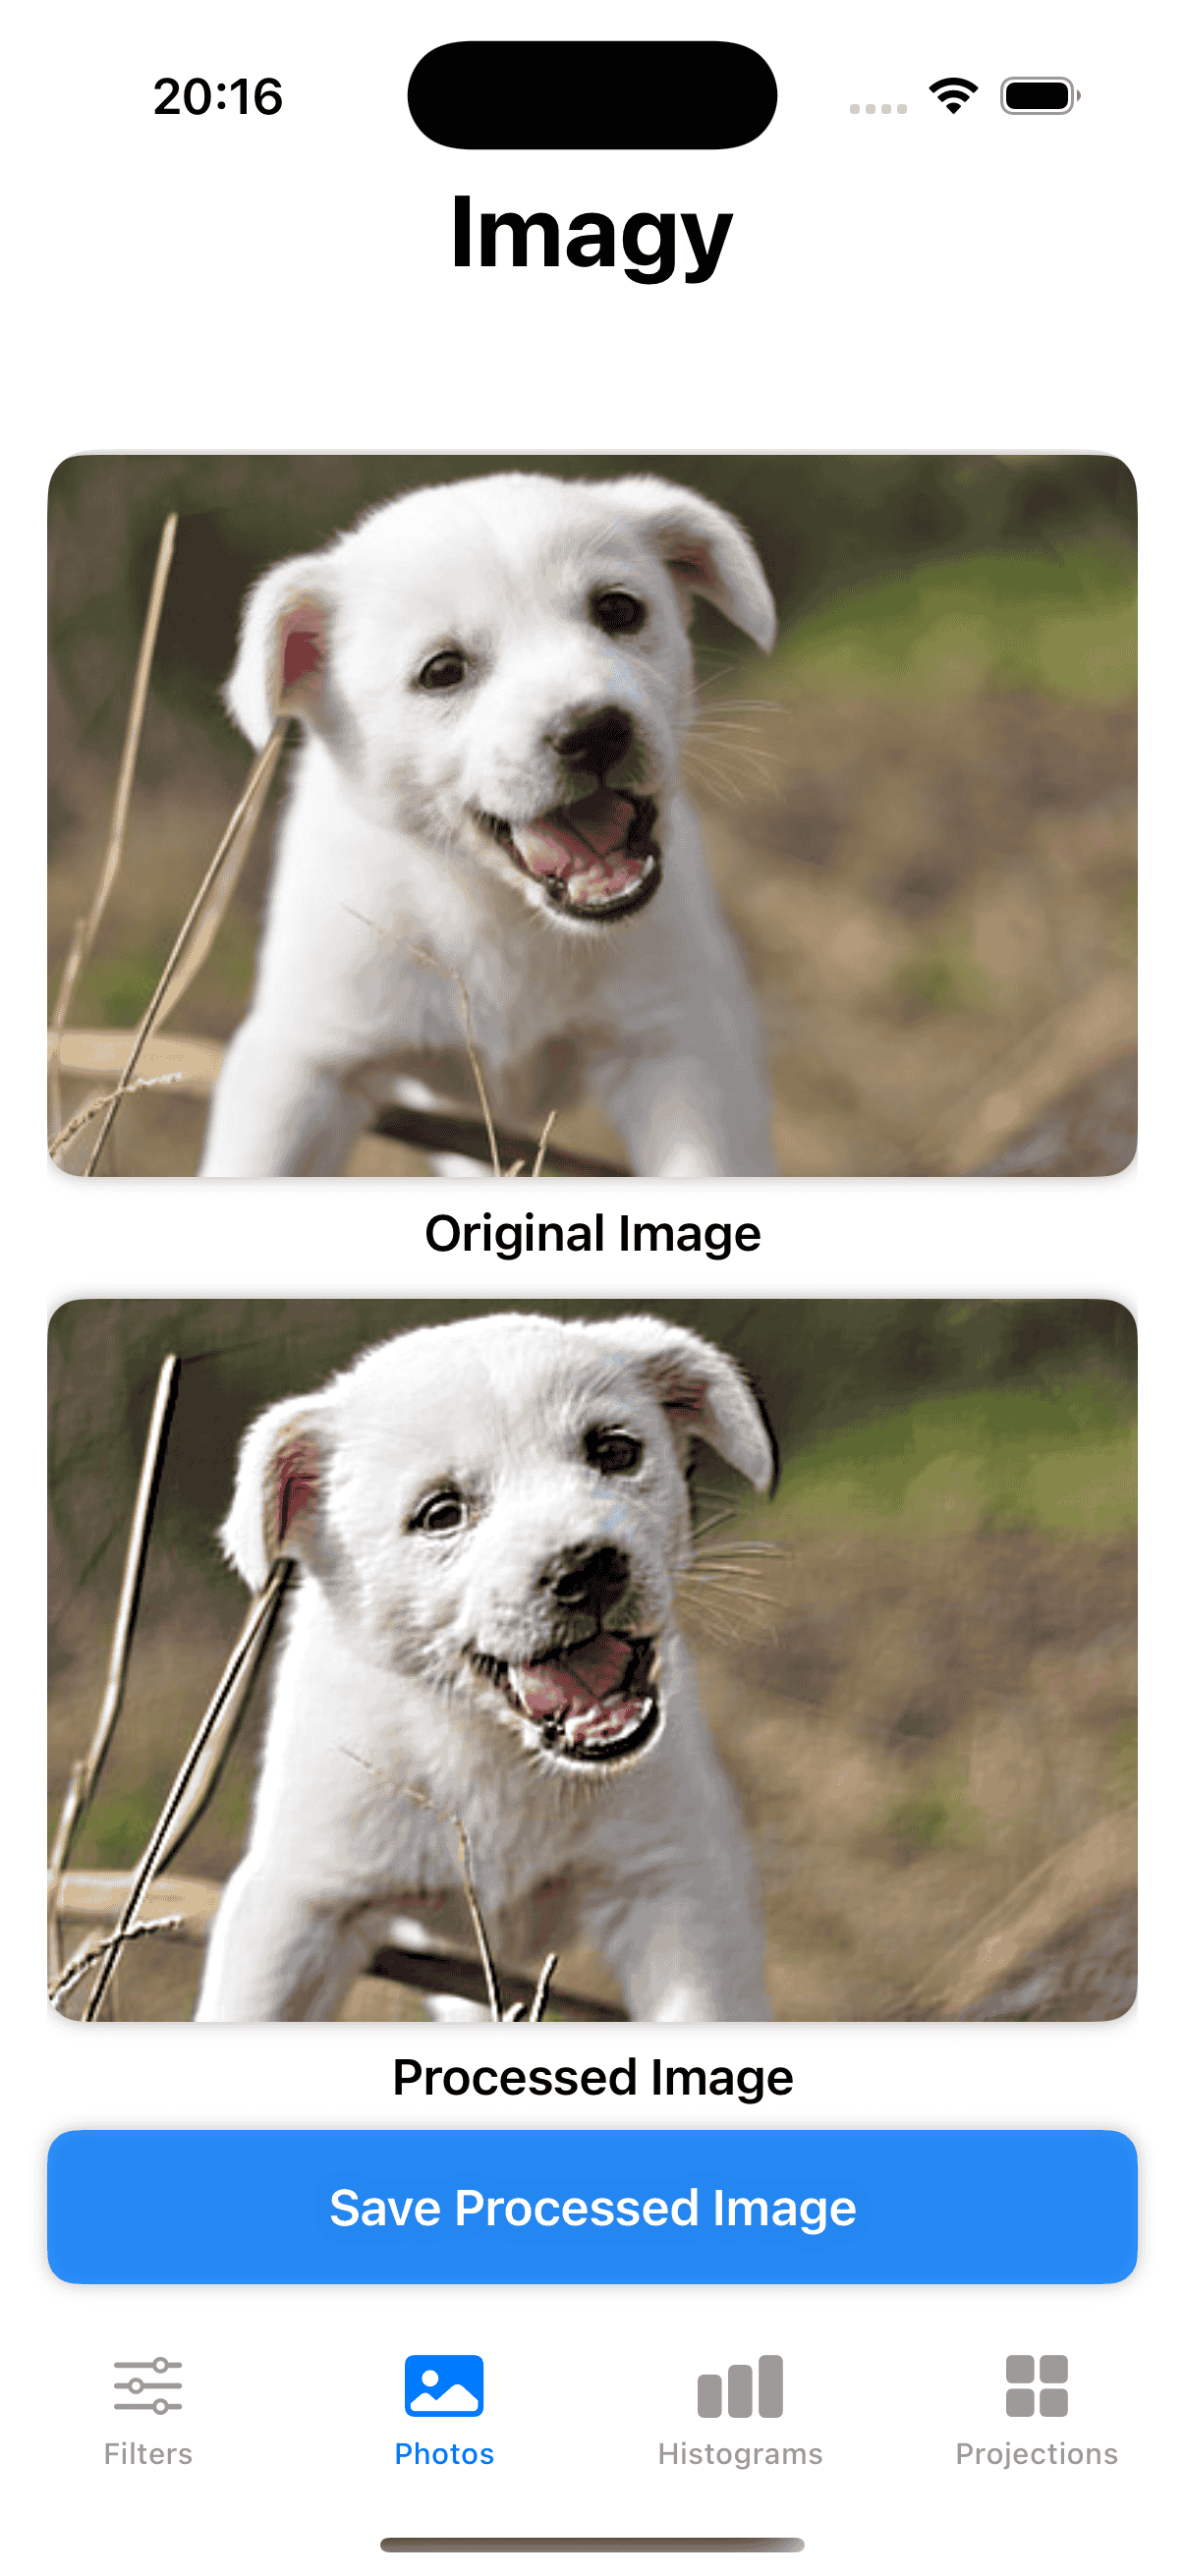
\includegraphics[width=\linewidth]{images/dog_embross_soft.png}
        \caption{kernelType=soft}
        \label{fig:dog_embross_soft}
    \end{subfigure}
    \hfill
    \begin{subfigure}{0.2\textwidth}
        \centering
        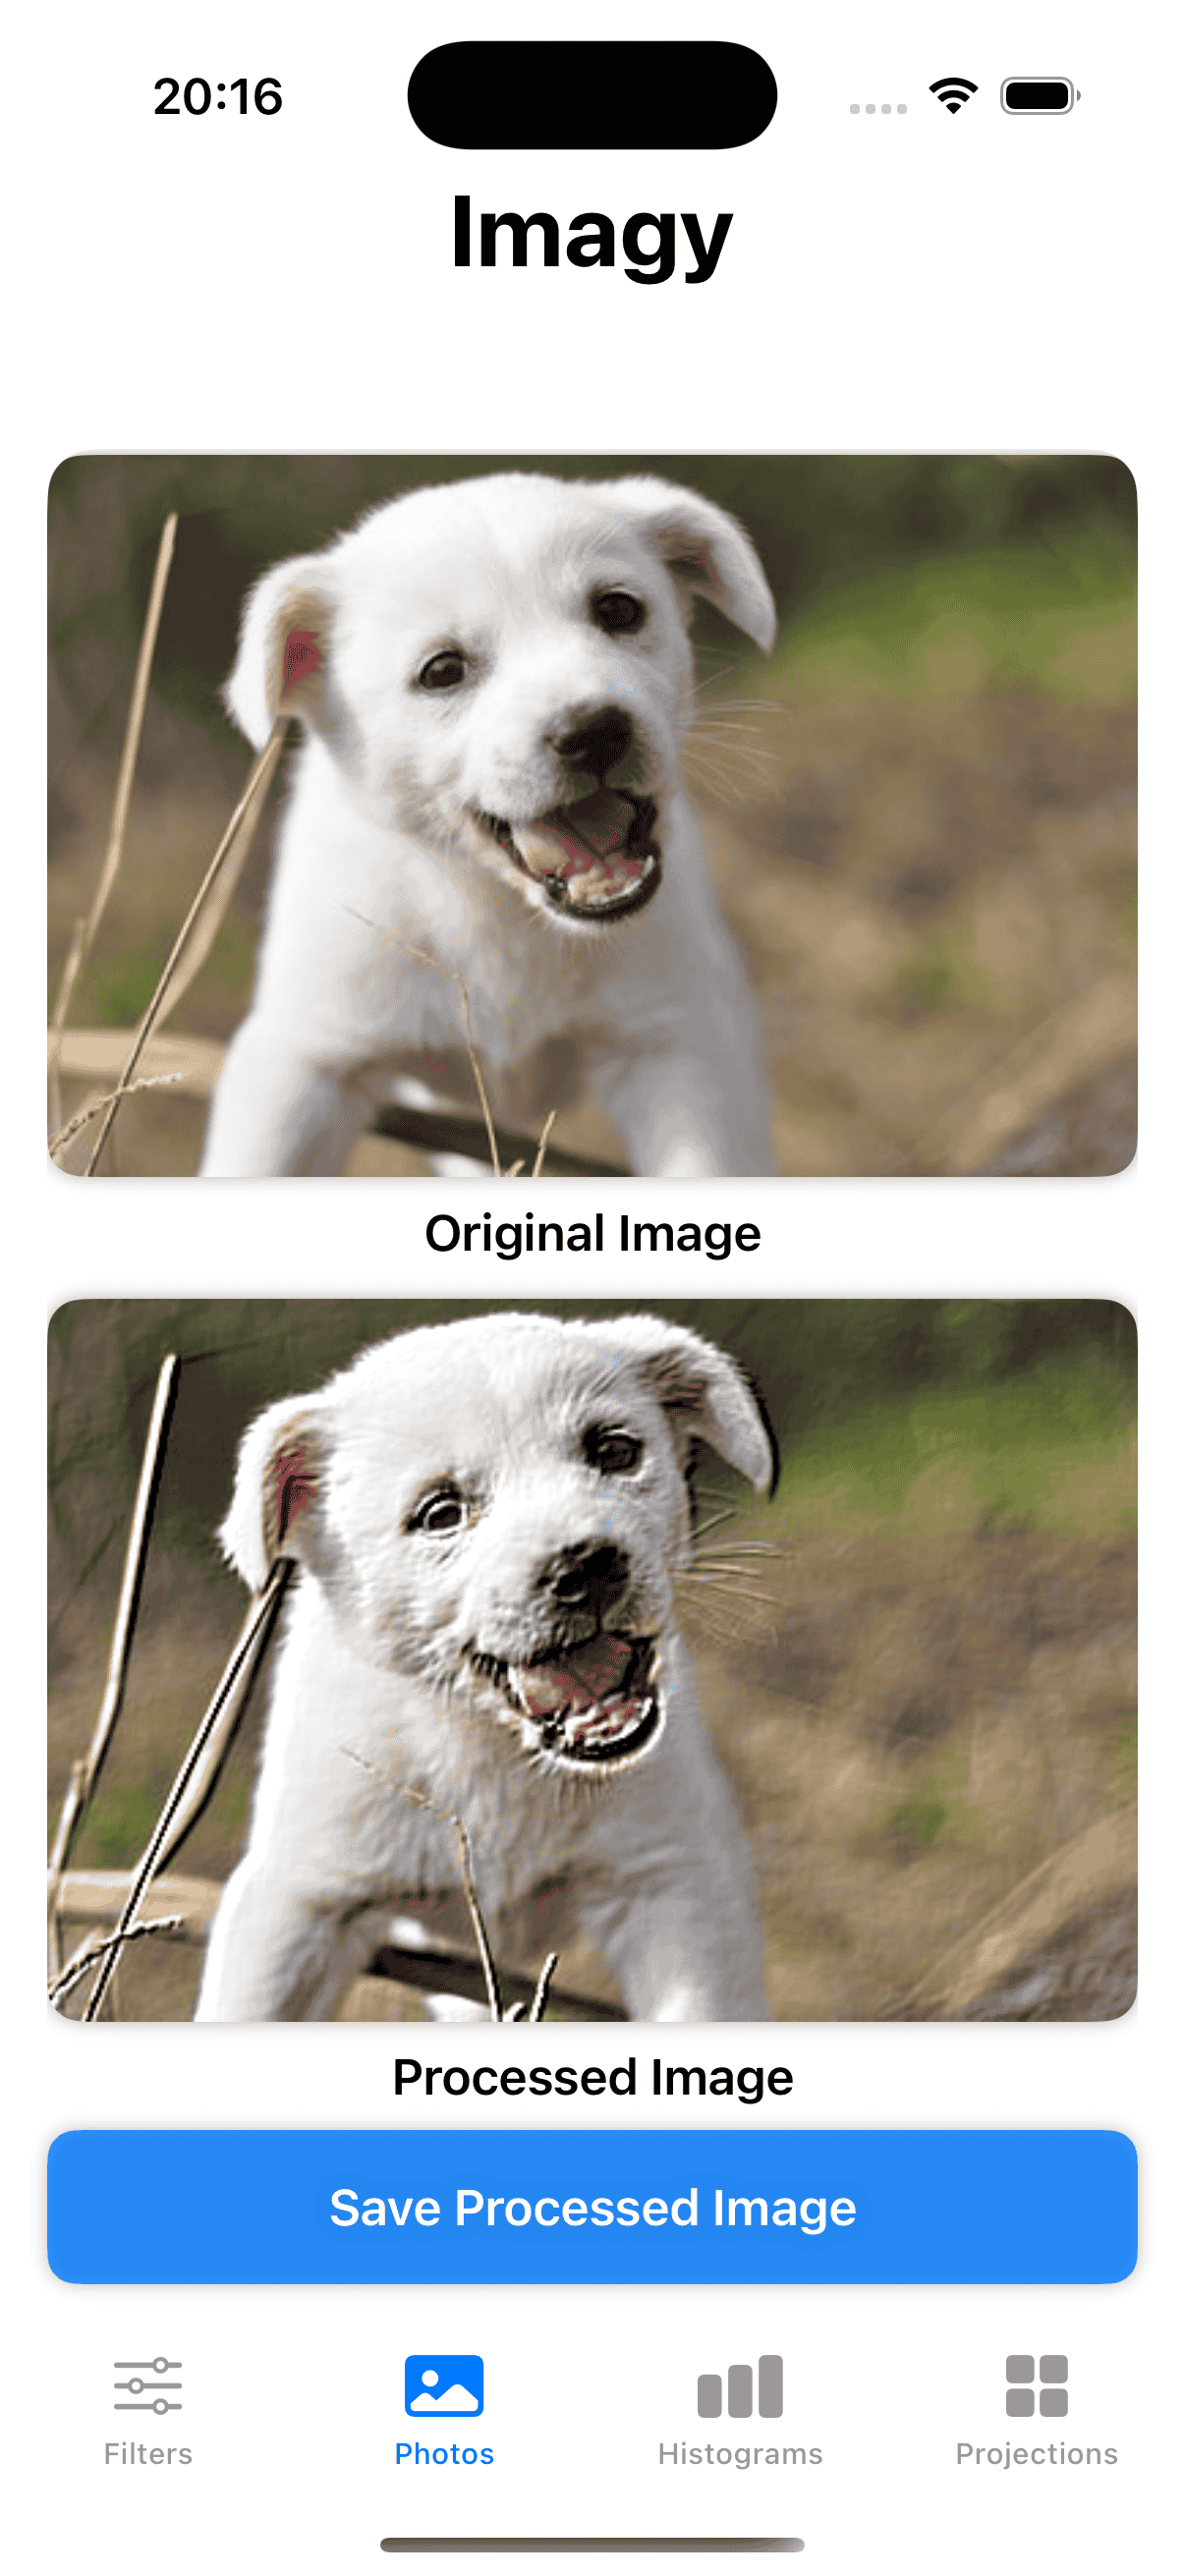
\includegraphics[width=\linewidth]{images/dog_embross_default.png}
        \caption{kernelType=default}
        \label{fig:dog_embross_default}
    \end{subfigure}
    \hfill
    \begin{subfigure}{0.2\textwidth}
        \centering
        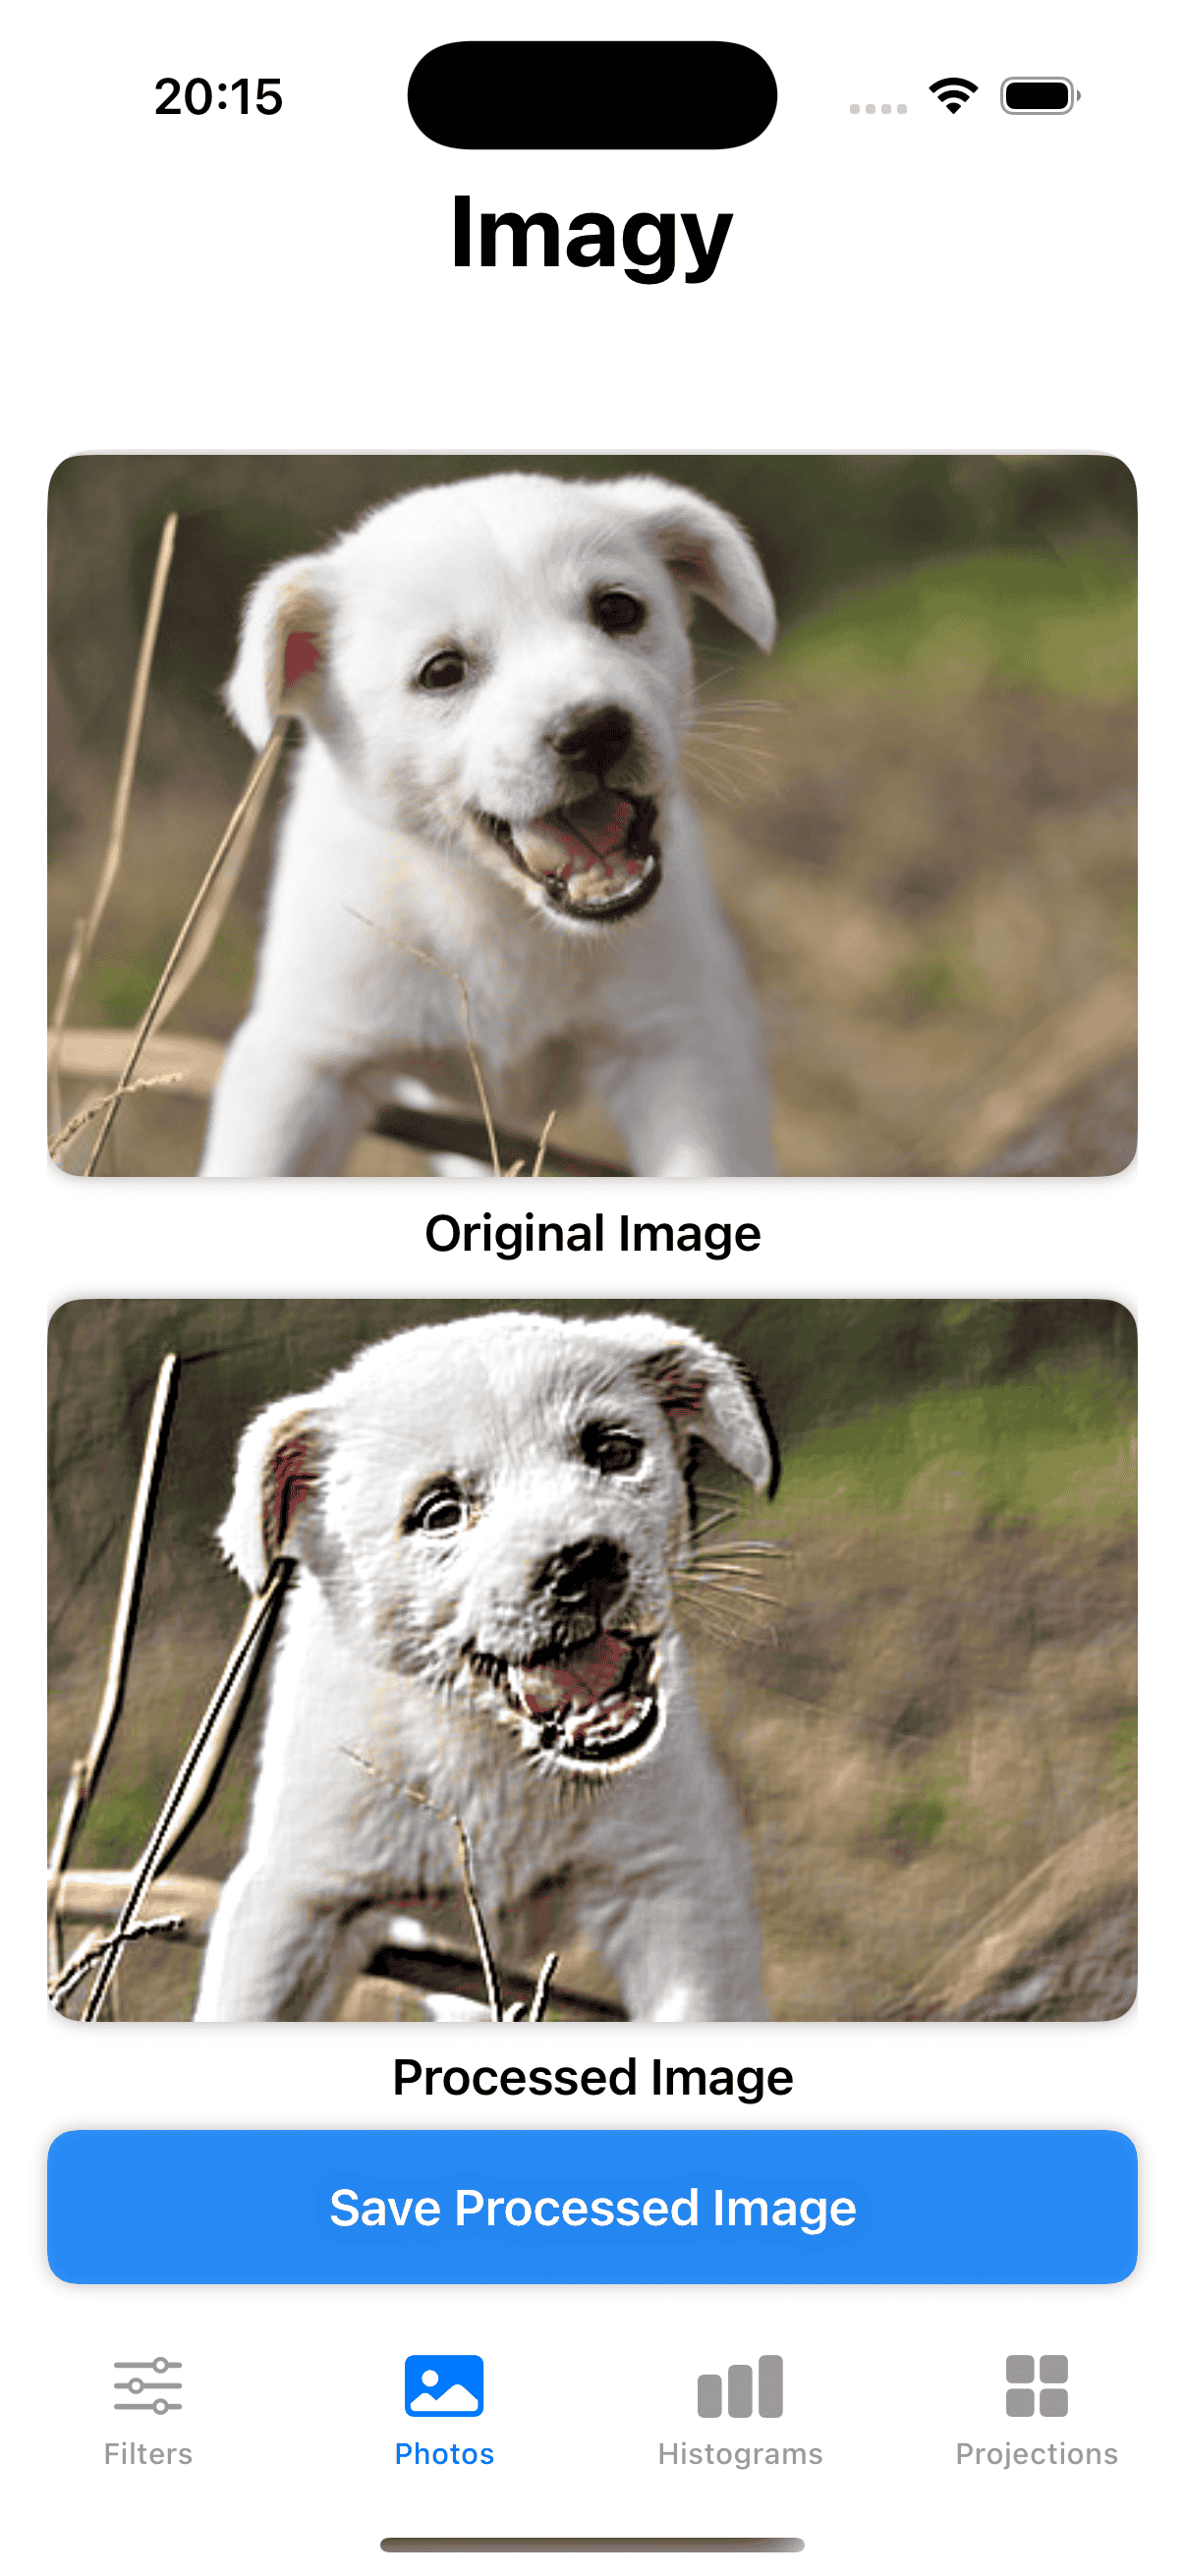
\includegraphics[width=\linewidth]{images/dog_embross_strong.png}
        \caption{kernelType=strong}
        \label{fig:dog_embross_strong}
    \end{subfigure}
    \caption{Embross filter - demonstracja. Widzimy różnice pomiędzy siłami kernela, strong powoduje największą transformację, wręcz zbyt dostrzegalną. Wybór opcji soft w tym wypadku może jednak dawać złudzenie trójwymiarowości futra.}
    \label{fig:embross}
\end{figure}

\subsection{FilmGrain}

\begin{itemize}
    \item \texttt{static var name: String = "Film Grain"}
    \item \texttt{grainStrength: Double} - defaultowo $0.2$, ograniczony do zakresu $0.0-1.0$ pobierany z widoku GUI ze stepem $0.01$. Dla każdego filtru losowany jest noise zgodnie z
          $$
              Int.random(in: -Int(grainStrength * 255)...Int(grainStrength * 255))
          $$
          a następnie dodawawany (ta sama wartość) do każdego kanału (prócz alpha, oczywiście ograniczając zakres do $0-255$)
    \item Jest to podstawowa wersja tego filtru, można go w przyszłości rozszerzyć o rozmiar ziarna, jego zakres czy różne wartości dla poszczególnych kanałów.
    \item Zastosowanie - fotografia i filmografia artystyczna (styl vintage, atmostfera), augumentacja danych do Computer Vision.
\end{itemize}

\begin{figure}[H]
    \centering
    \begin{subfigure}{0.2\textwidth}
        \centering
        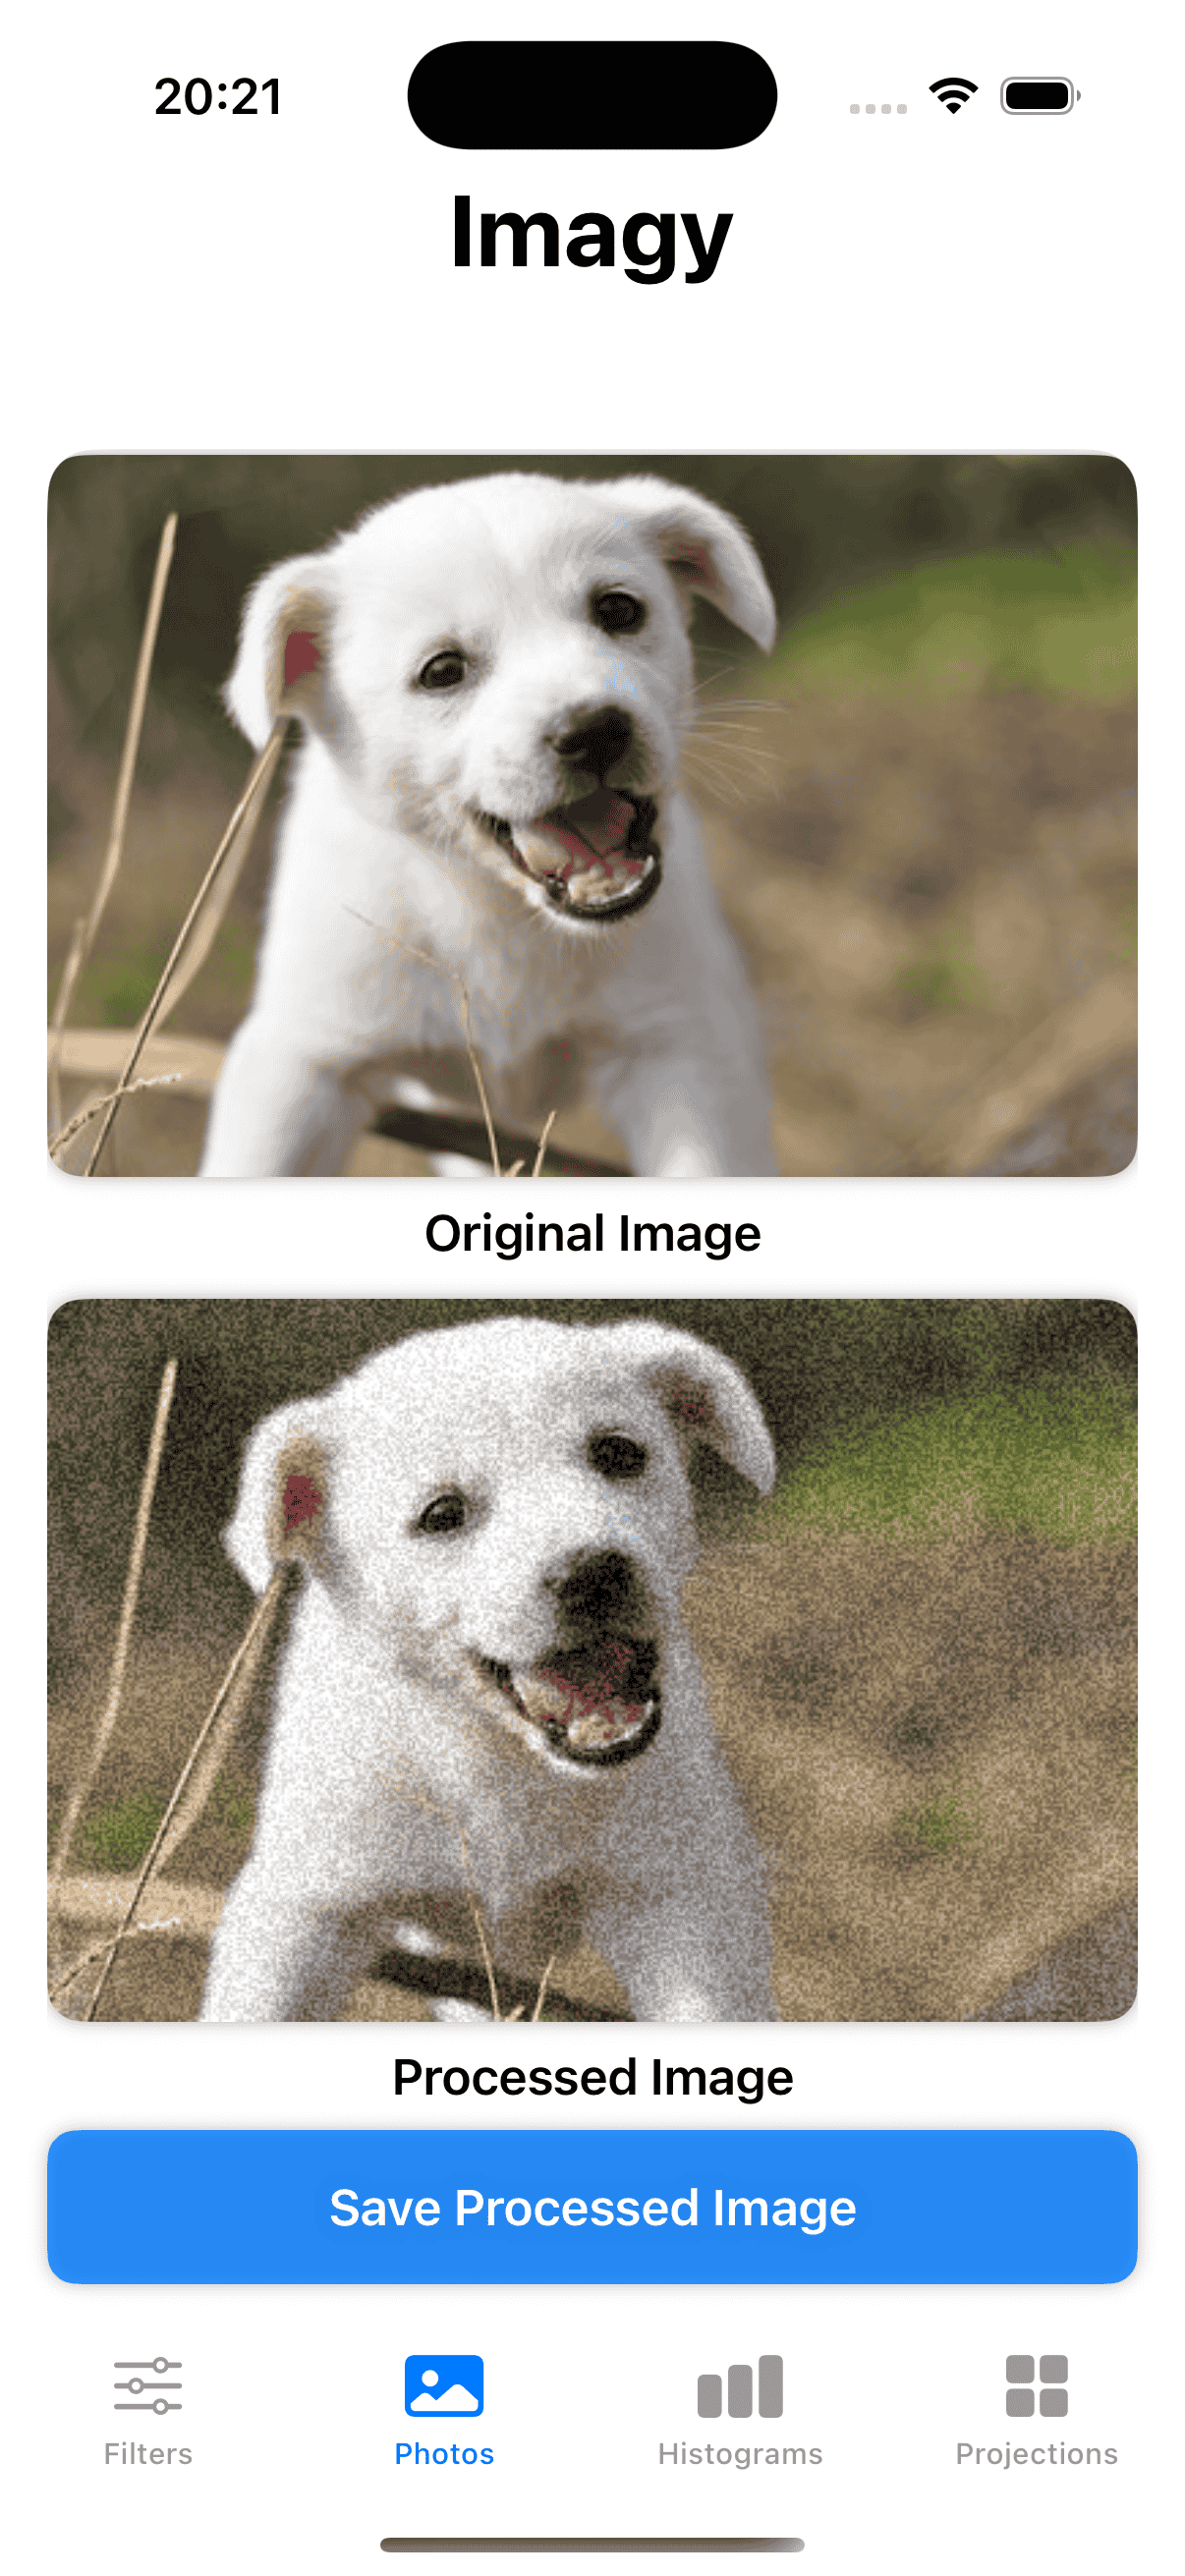
\includegraphics[width=\linewidth]{images/dog_film_grain_0.1.png}
        \caption{grainStrength=0.1}
        \label{fig:dog_film_grain_0}
    \end{subfigure}
    \hfill
    \begin{subfigure}{0.2\textwidth}
        \centering
        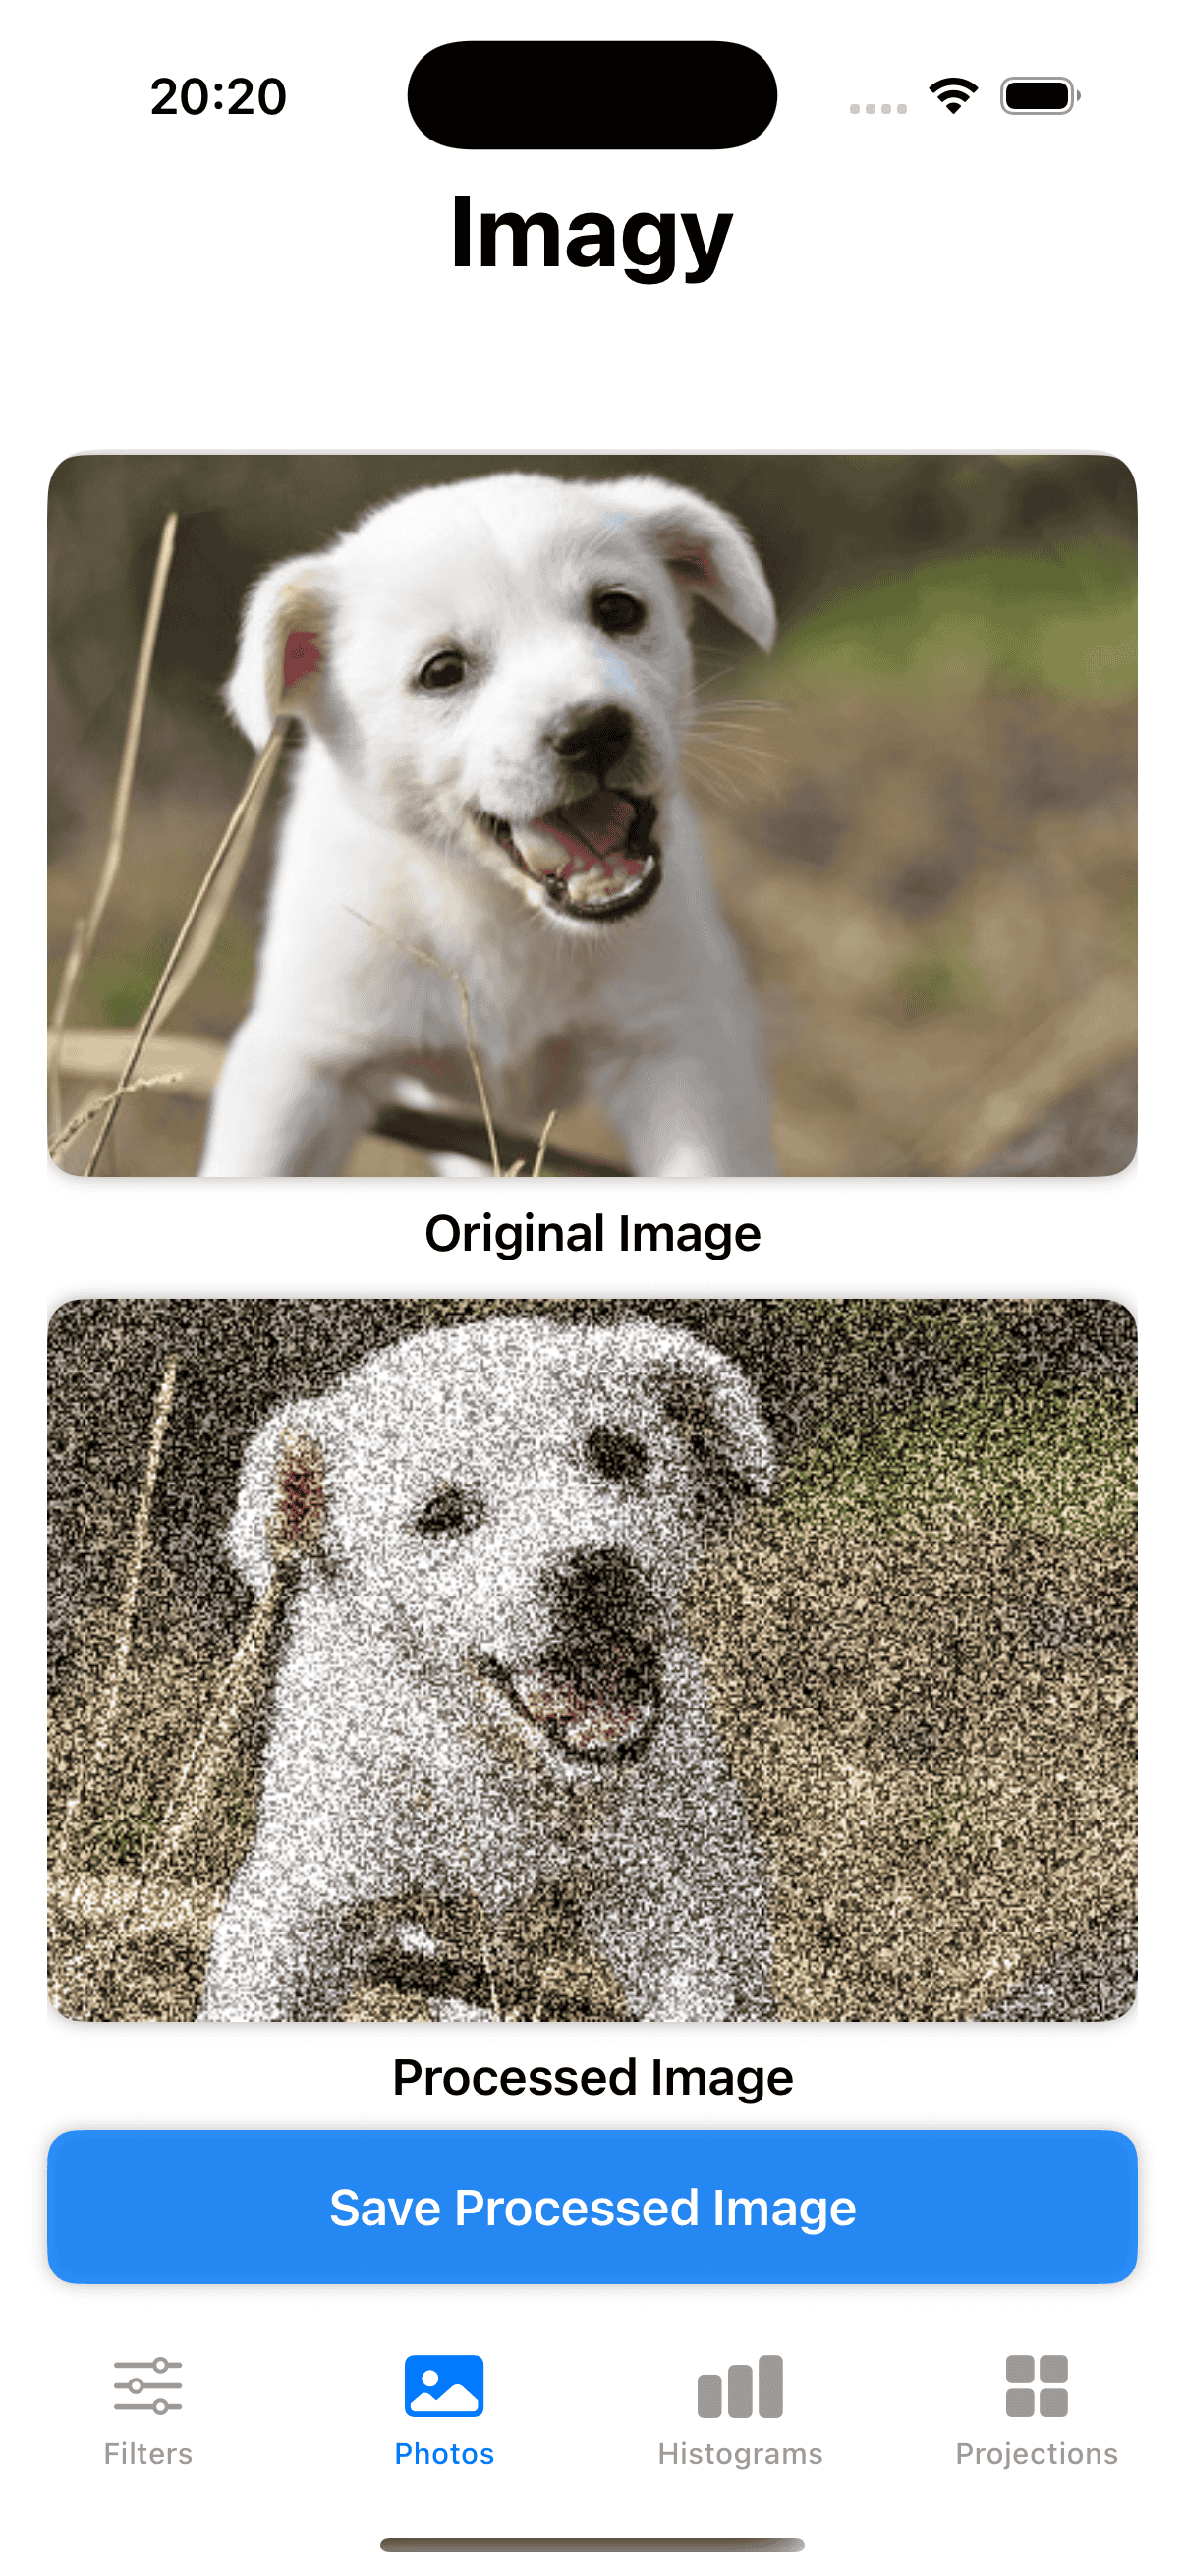
\includegraphics[width=\linewidth]{images/dog_film_grain_0.5.png}
        \caption{grainStrength=0.5}
        \label{fig:dog_film_grain_0}
    \end{subfigure}
    \hfill
    \begin{subfigure}{0.2\textwidth}
        \centering
        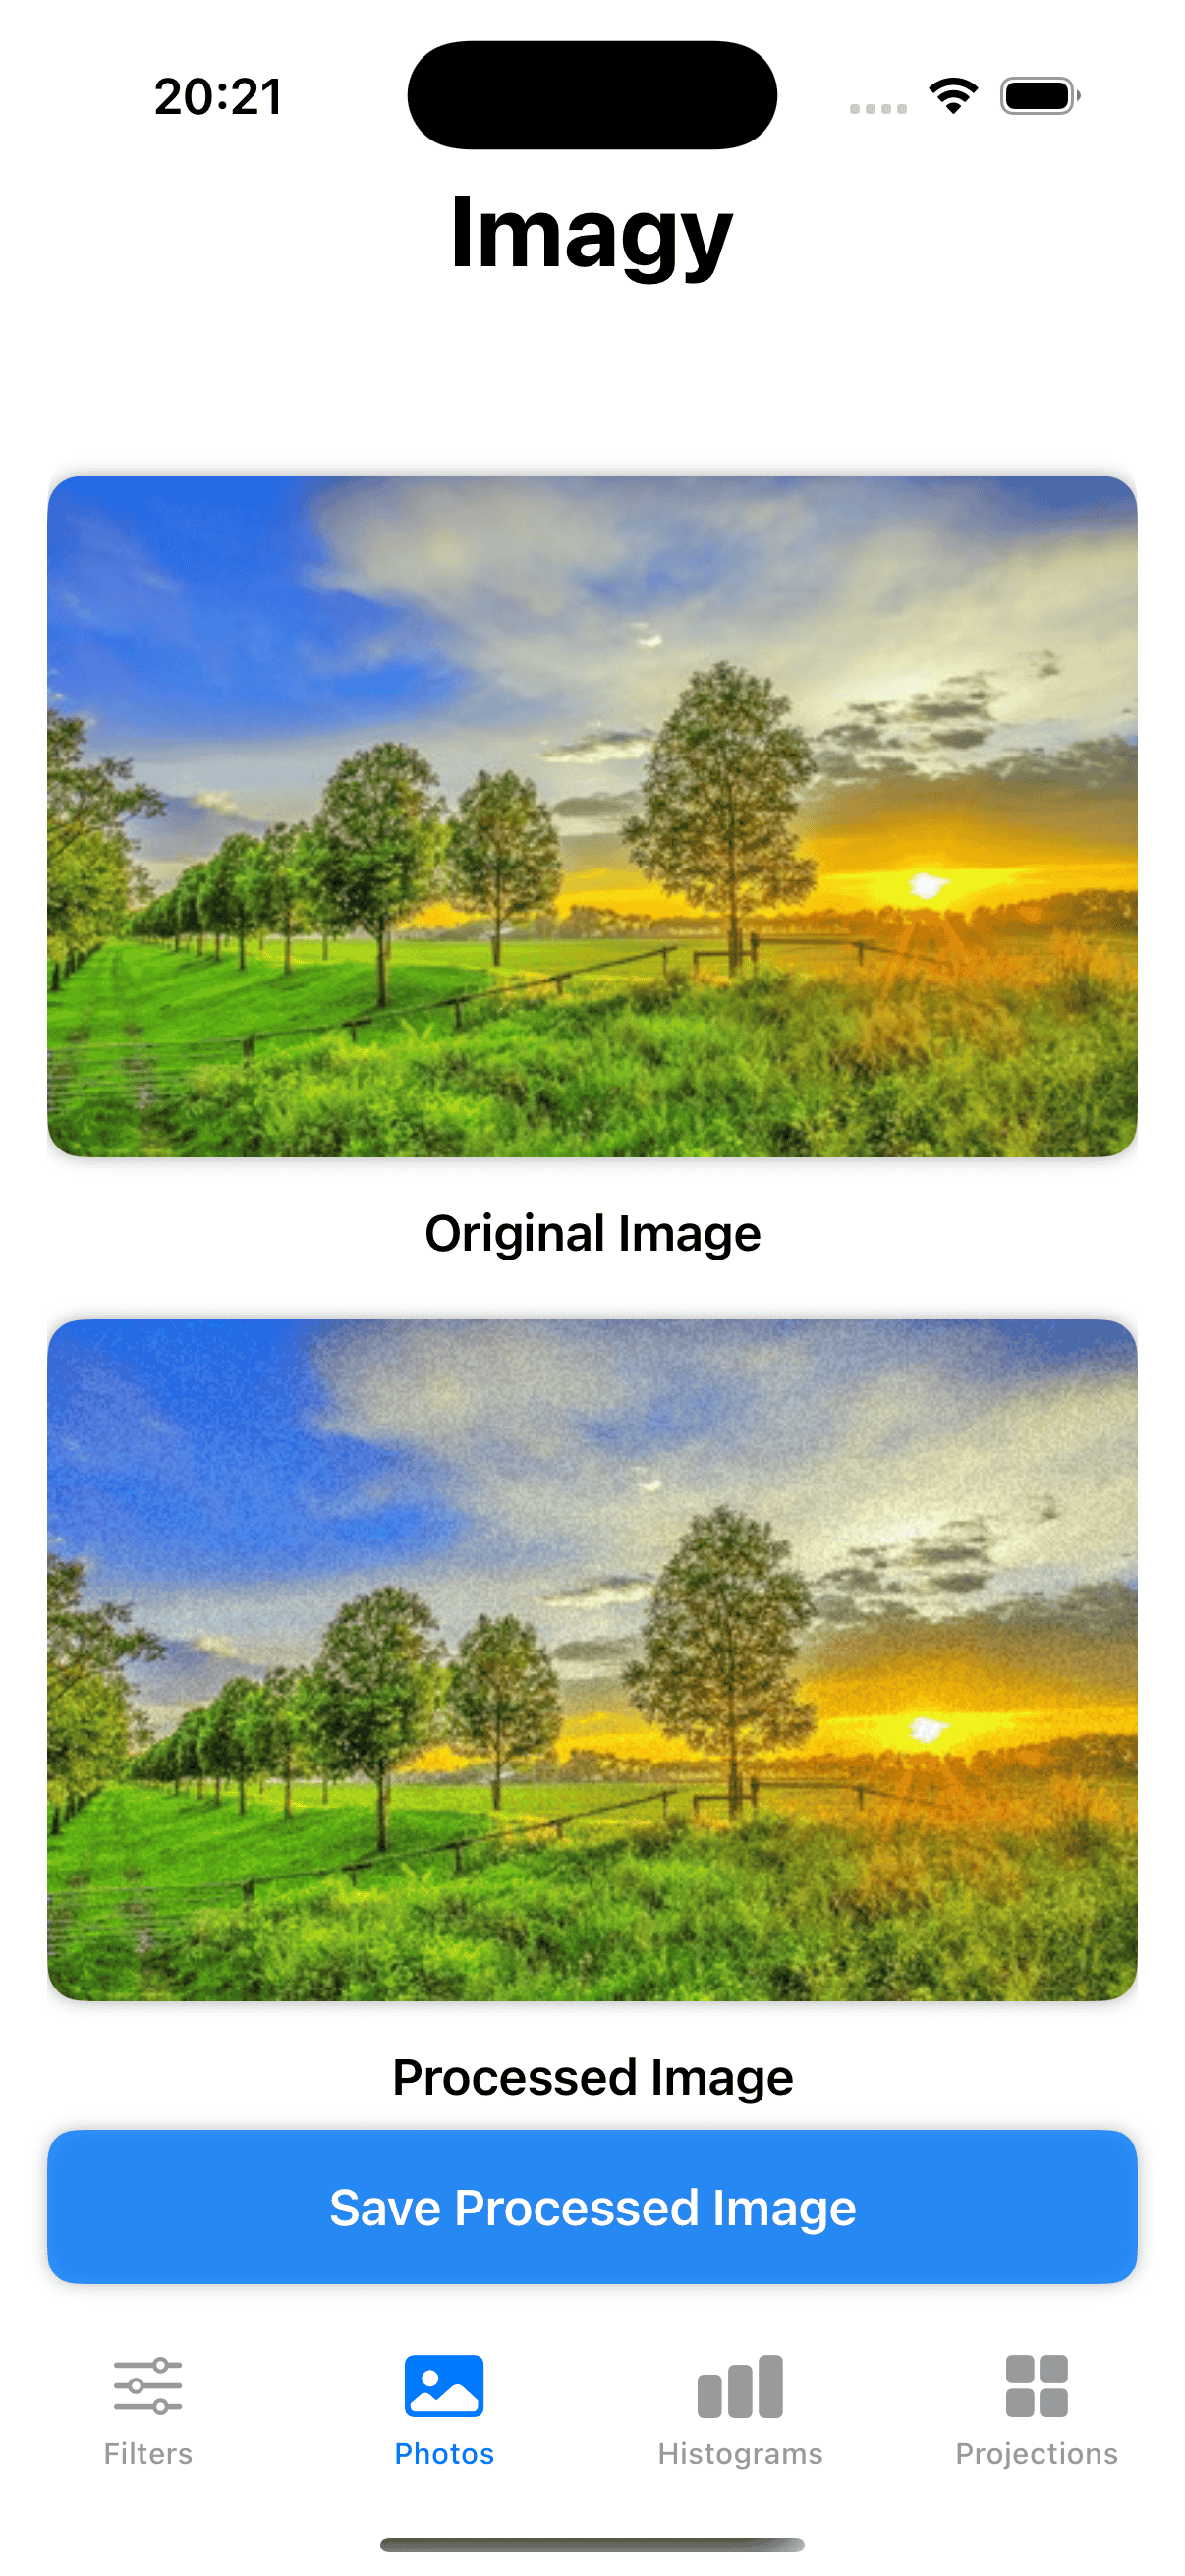
\includegraphics[width=\linewidth]{images/trees_film_grain_0.06.png}
        \caption{grainStrength=0.06}
        \label{fig:trees_film_grain_0}
    \end{subfigure}
    \hfill
    \begin{subfigure}{0.2\textwidth}
        \centering
        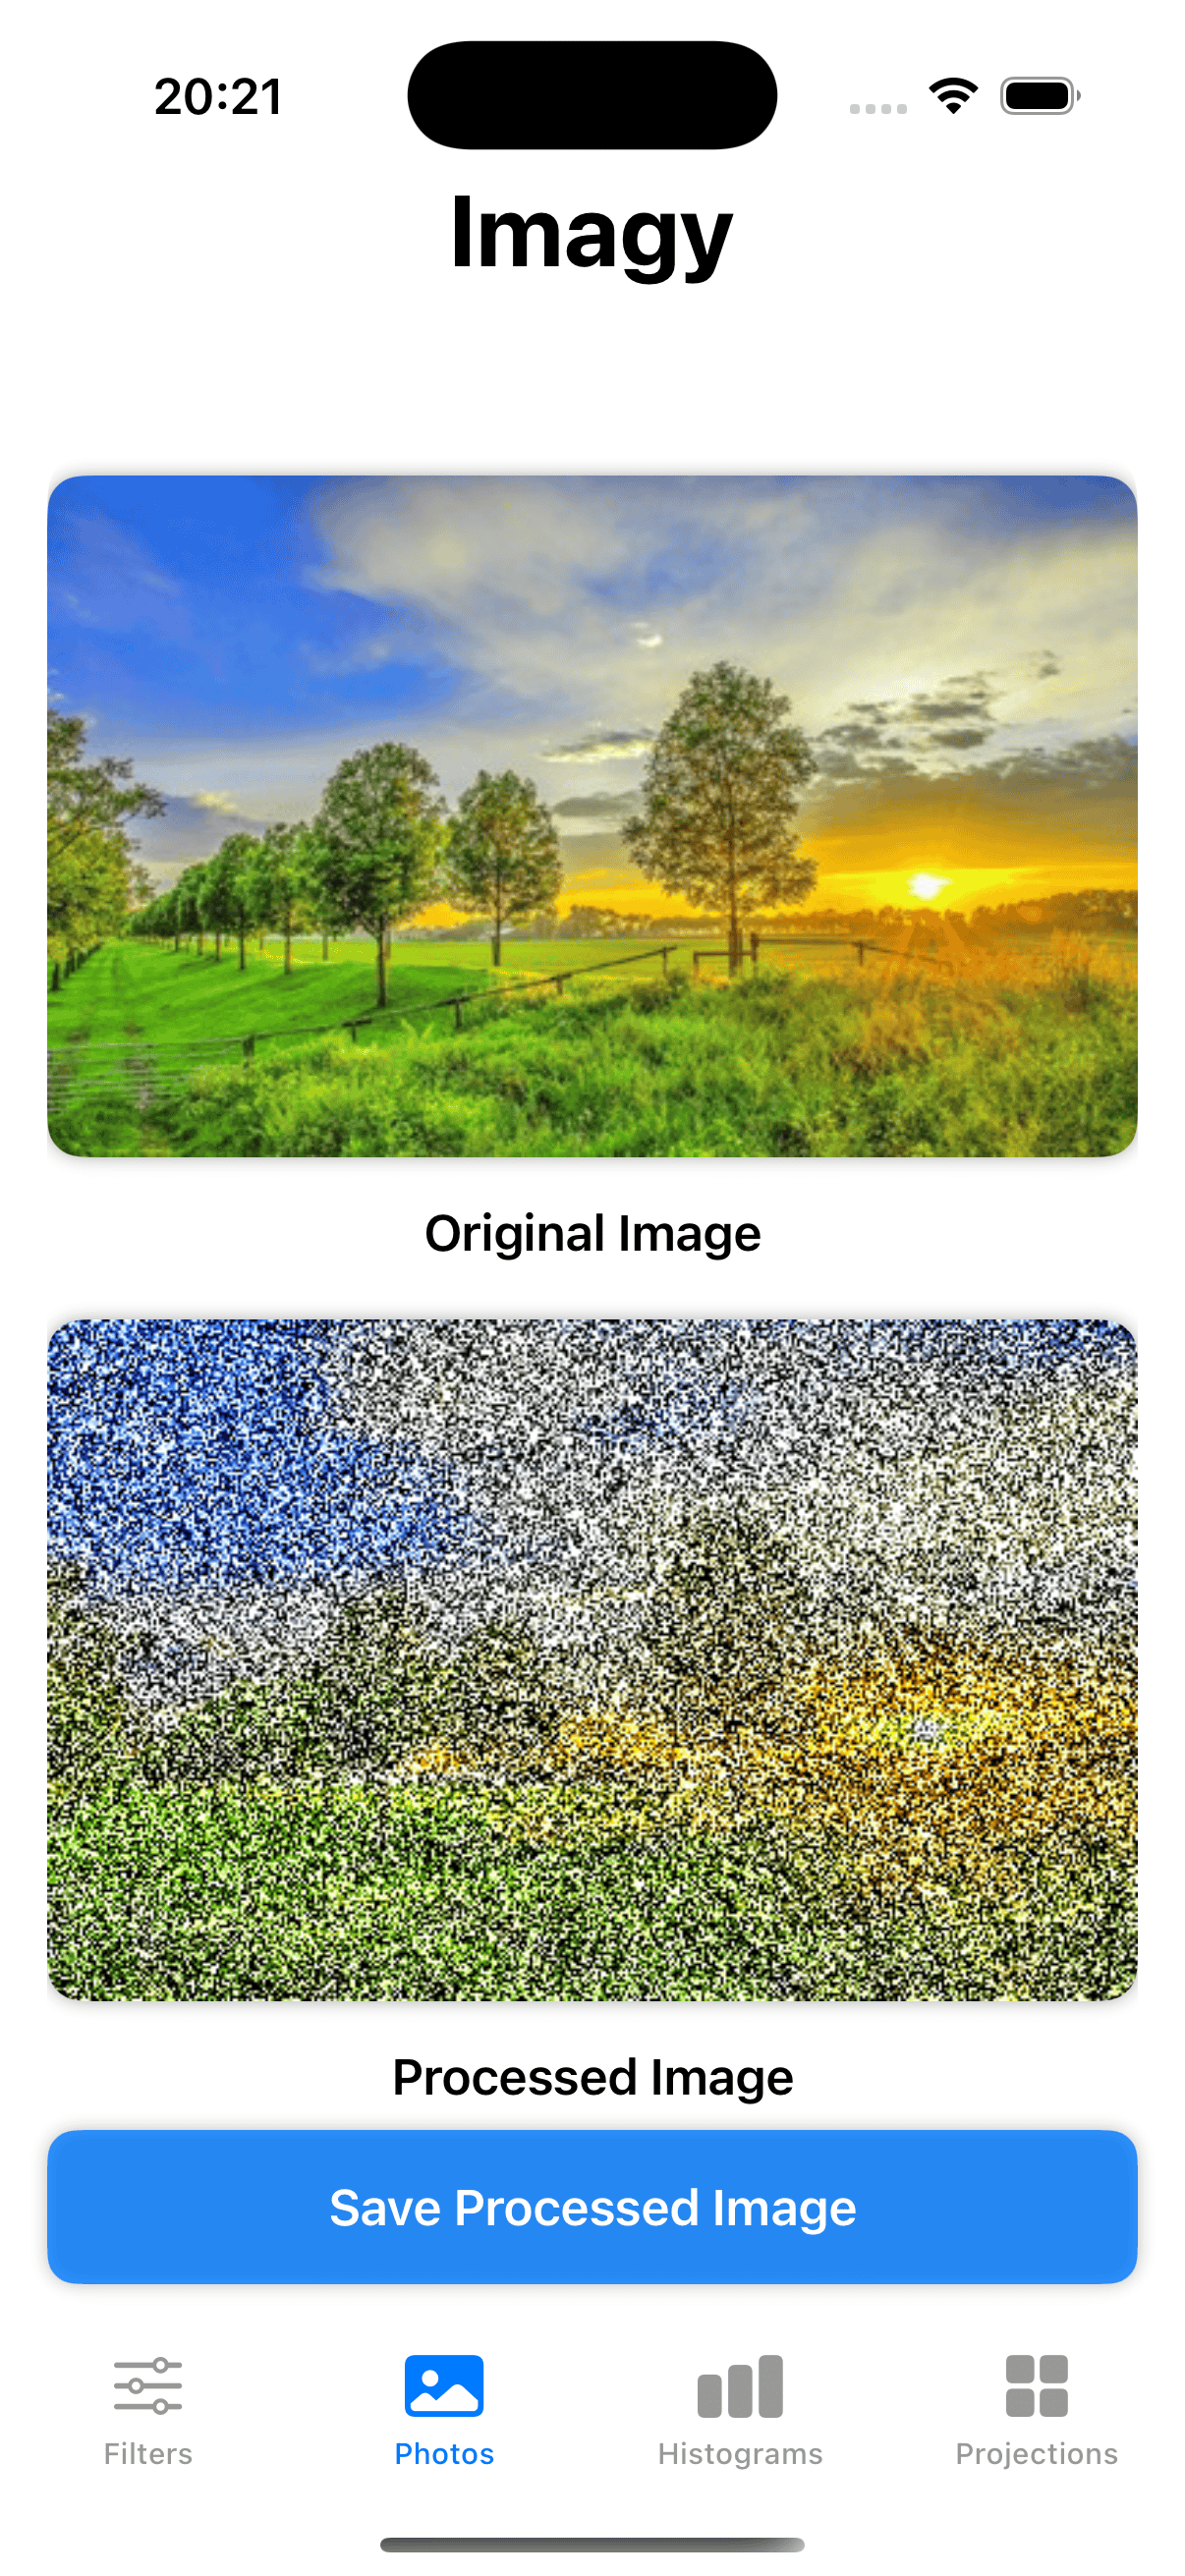
\includegraphics[width=\linewidth]{images/trees_film_grain_1.0.png}
        \caption{grainStrength=1.0}
        \label{fig:trees_film_grain_1}
    \end{subfigure}
    \caption{Film Grain filter - demonstracja. Wartość $1.0$ produkuje obraz kompletnie nieczytelny, ledwo widać co na nim jest. Wartości 0.5 są konkretnie saszumione. Wartości poniżej $0.1$ pozostają ledwo dostrzegalne, przypominając zakłucenia znane ze starych teleskopowych telewizorów.}
    \label{fig:film_grain}
\end{figure}

\subsection{Gaussian}

\begin{itemize}
    \item \texttt{static var name: String = "Averaging"}
    \item \texttt{kernelSize: Int} - wymiar jądra filtru, domyślnie $3$, pobierany z widoku GUI ograniczony do wartości nieparzystych z zakresu $3-21$.
    \item \texttt{sigma: Float} - odchylenie standardowe rozkładu normalnego domyślnie $1.0$, pobierany z widoku GUI ograniczony do wartości z zakresu $0.1-3.0$ z krokiem $0.1$.
    \item Przykładowe jądro generowane przez program:
          $$
              \frac{1}{16}
              \begin{bmatrix}
                  1 & 2 & 1 \\
                  2 & 4 & 2 \\
                  1 & 2 & 1
              \end{bmatrix}
          $$
    \item \texttt{static func generateGaussianKernel(size: Int, sigma: Float) -> [[Float]]} - generuje macierz jądra filtru o wymiarze \texttt{size}x\texttt{size} zawierającą wartości losowane wartości z rozkładu normalnego z parametrami zależnymi od odległości od środka kernela, unormalnizowane by cały kernel element-wise się sumował do 1.
    \item Rozmycie obrazu (używane do odszumiania i zwiększania jakości poprzez ukrywanie niedoskonałości), używany do przetwarzania obrazów w detekcji krawędzi.
\end{itemize}

\begin{figure}[H]
    \centering
    \begin{subfigure}{0.2\textwidth}
        \centering
        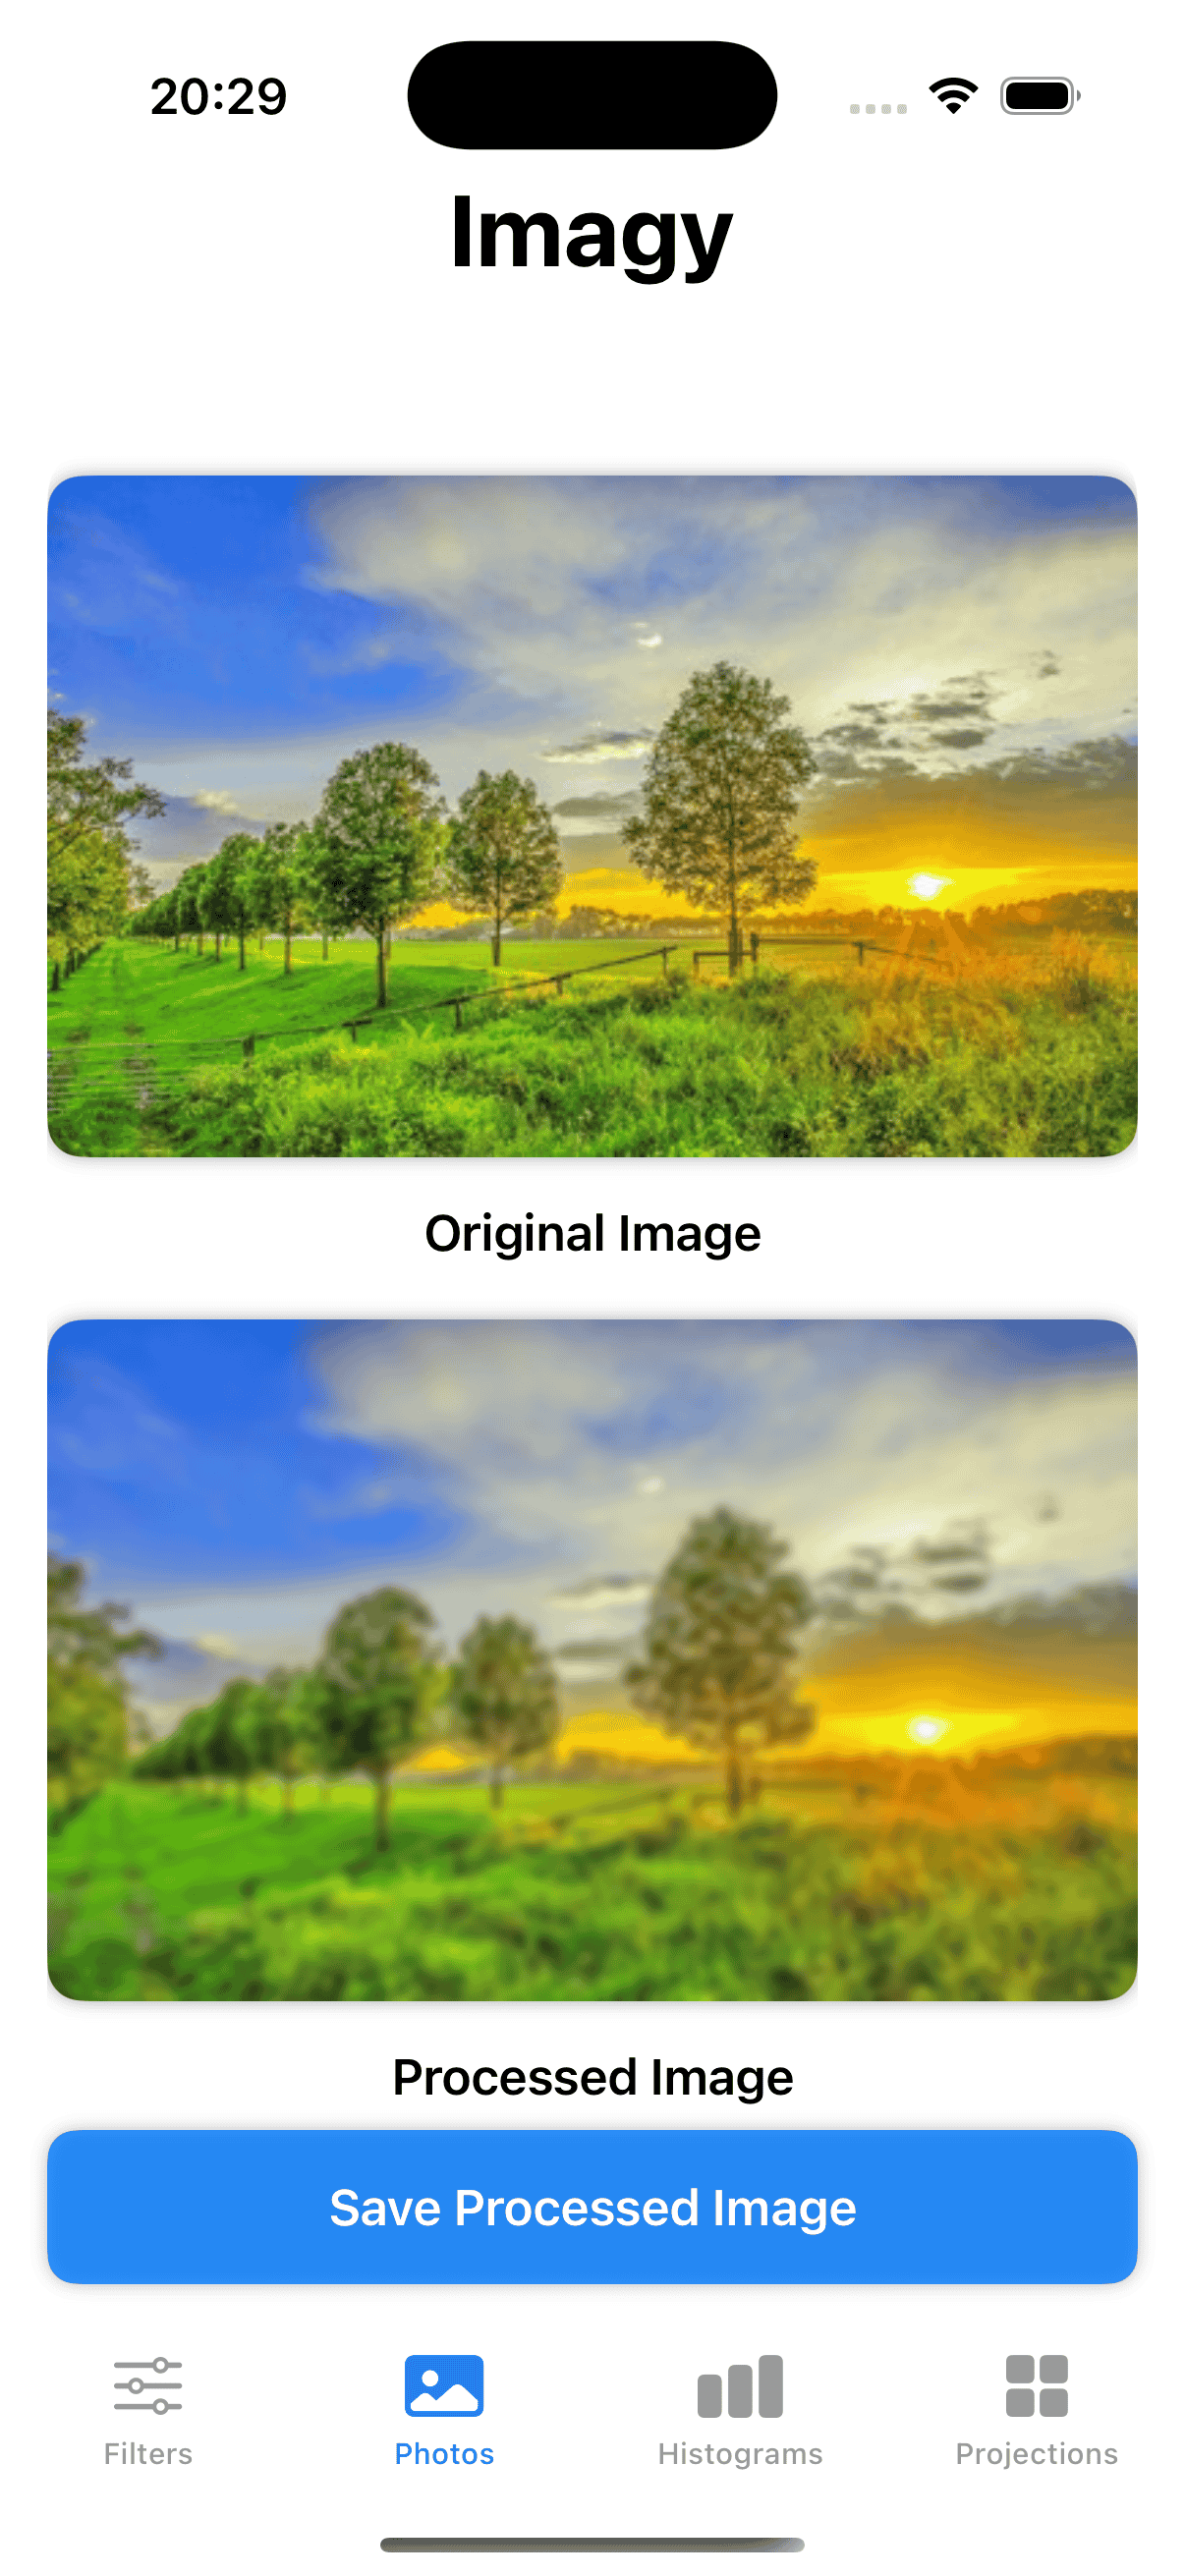
\includegraphics[width=\linewidth]{images/trees_gaussian_7_1.8.png}
        \caption{kernelSize=7, sigma=1.8}
        \label{fig:trees_gaussian_7_1}
    \end{subfigure}
    \begin{subfigure}{0.2\textwidth}
        \centering
        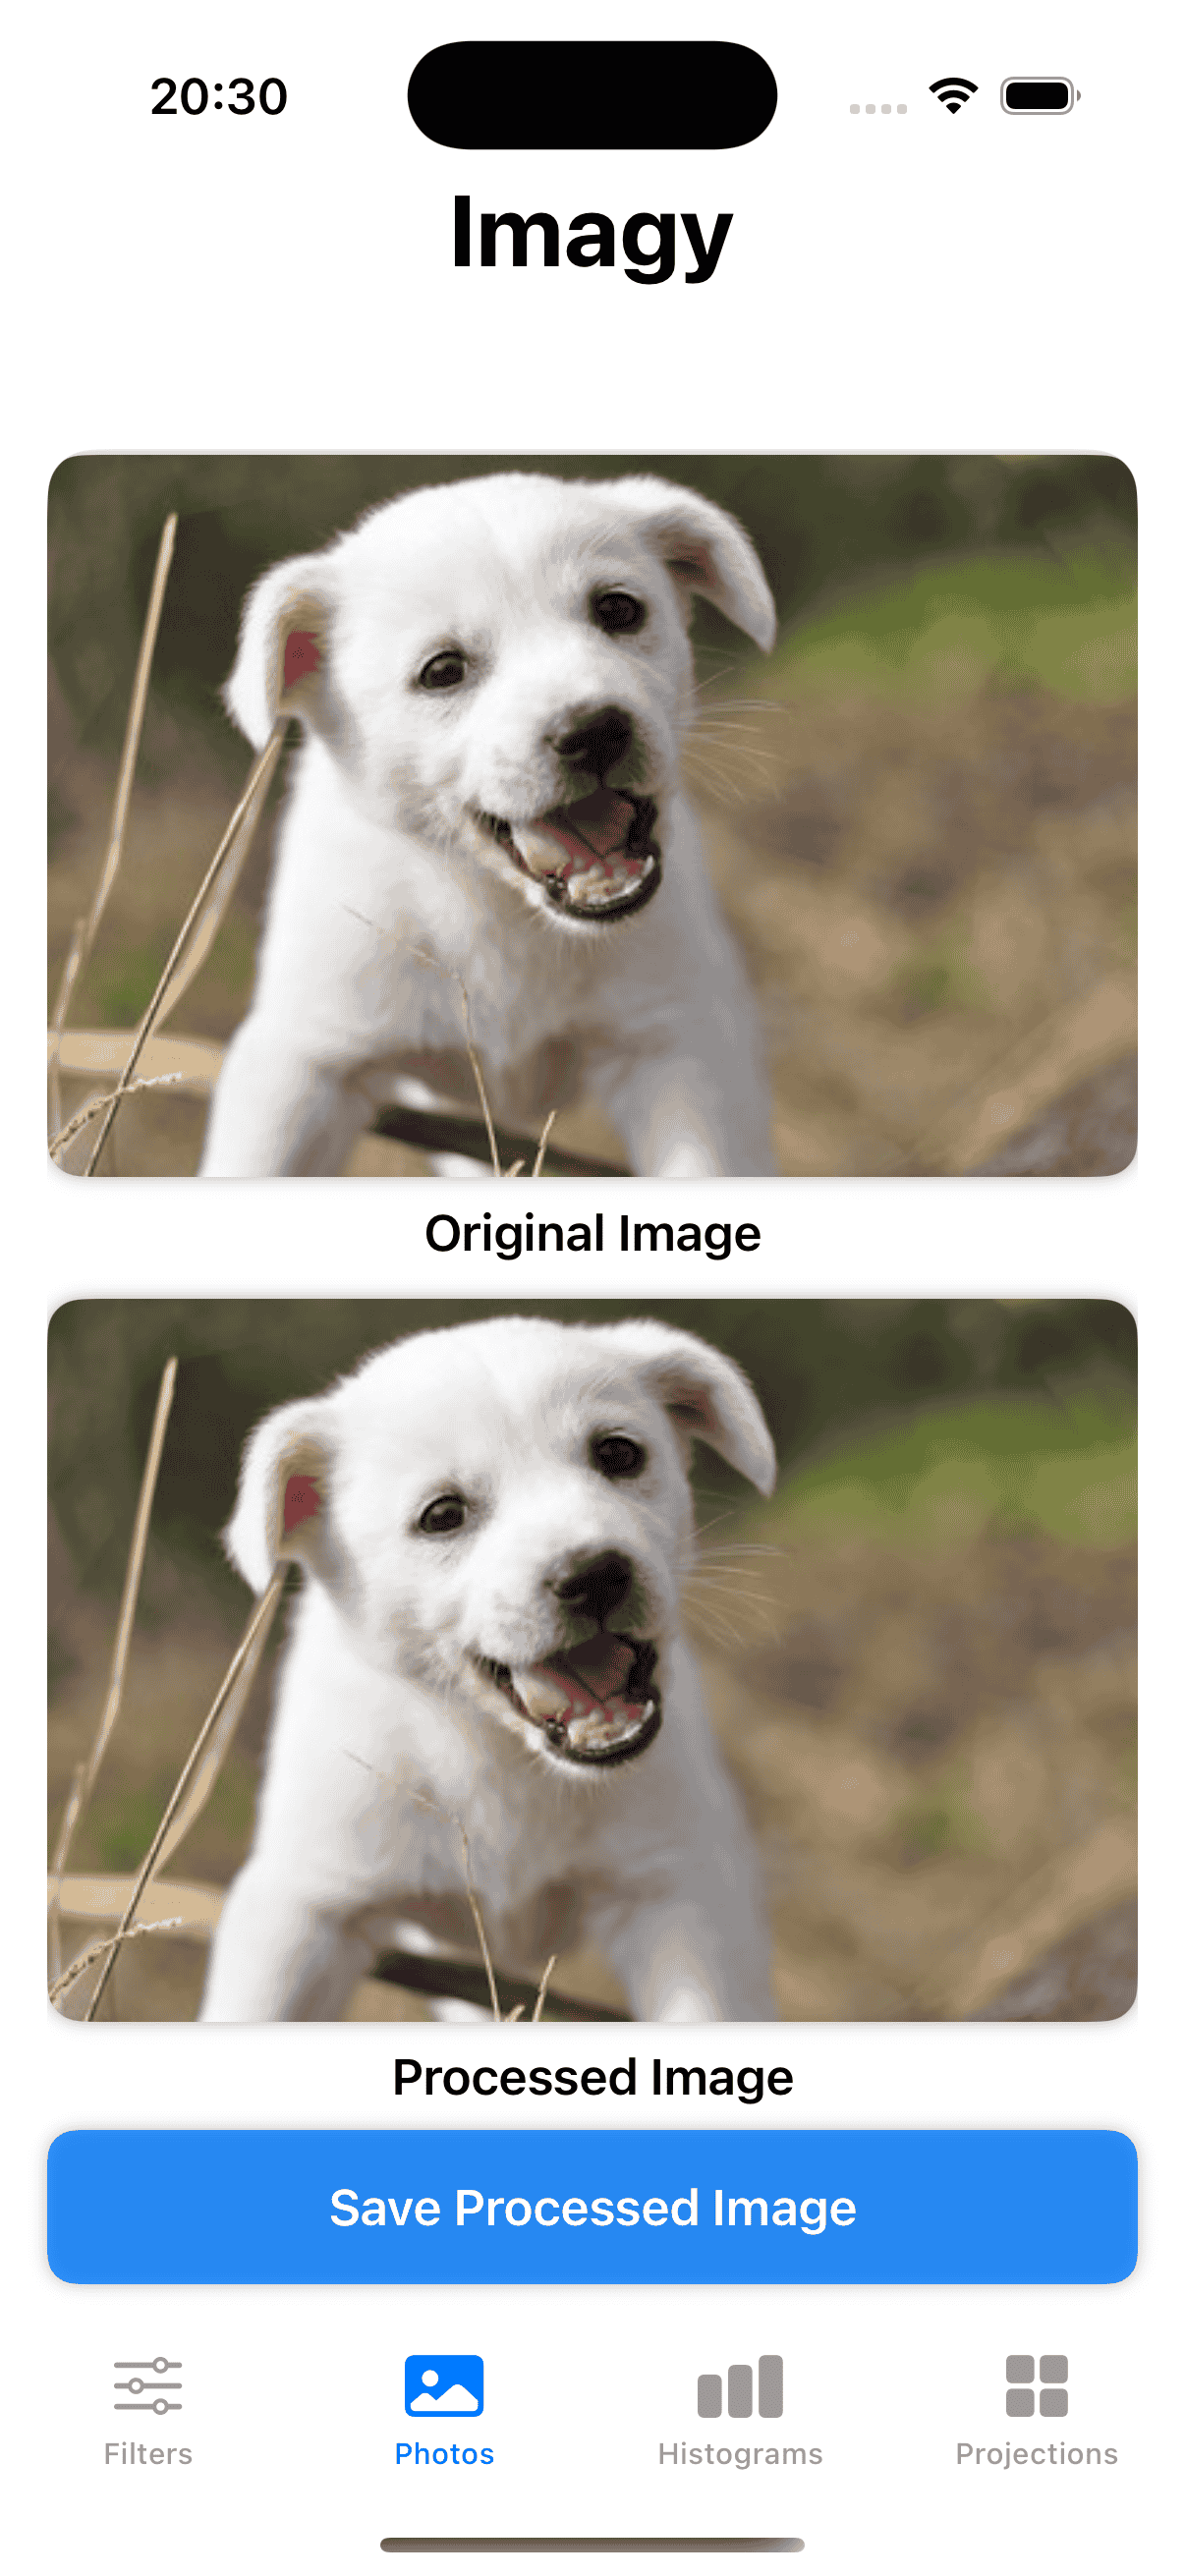
\includegraphics[width=\linewidth]{images/dog_gaussian_5_0.3.png}
        \caption{kernelSize=5, sigma=0.3}
        \label{fig:dog_gaussian_5_0}
    \end{subfigure}
    \caption{Gaussian Blur filter - demonstracja. Na lewo zdjęcie z bardzo mocną transformacją powodującą znaczące rozmazanie się obrazka, jednak w przeciwieństwie do \ref{fig:trees_averaging_21} rozmazanie to nie sprawia wrażenia że zdjęcie jest poruszone. Na prawo słabszy kernel, powodujący lekkie zlanie się detali futra psa (trzeba się przyjrzeć by zobaczyć zmienę, choć ludzkie oko od razu widzi że te zdjęcia nie są identyczne).}
    \label{fig:gaussian}
\end{figure}

\subsection{Glitch}

\begin{itemize}
    \item \texttt{static var name: String = "Glitch"}
    \item Działanie:
          \begin{enumerate}
              \item Dla każdego wiersza losujemy wartość z zakresu $-5...5$ i zamieniamy te wiersze pozycjami
              \item Dla każdego piksela losujemy (dla każdego z kanałów koloru oddzielnie) wartość z zakresu $-20...20$ i dodajemy do wartości piksela (oczywiście ograniczając wartości do $0...255$)
          \end{enumerate}
    \item Zastosowanie - tworzenie sztuki, gry video.
\end{itemize}

\begin{figure}[H]
    \centering
    \begin{subfigure}{0.2\textwidth}
        \centering
        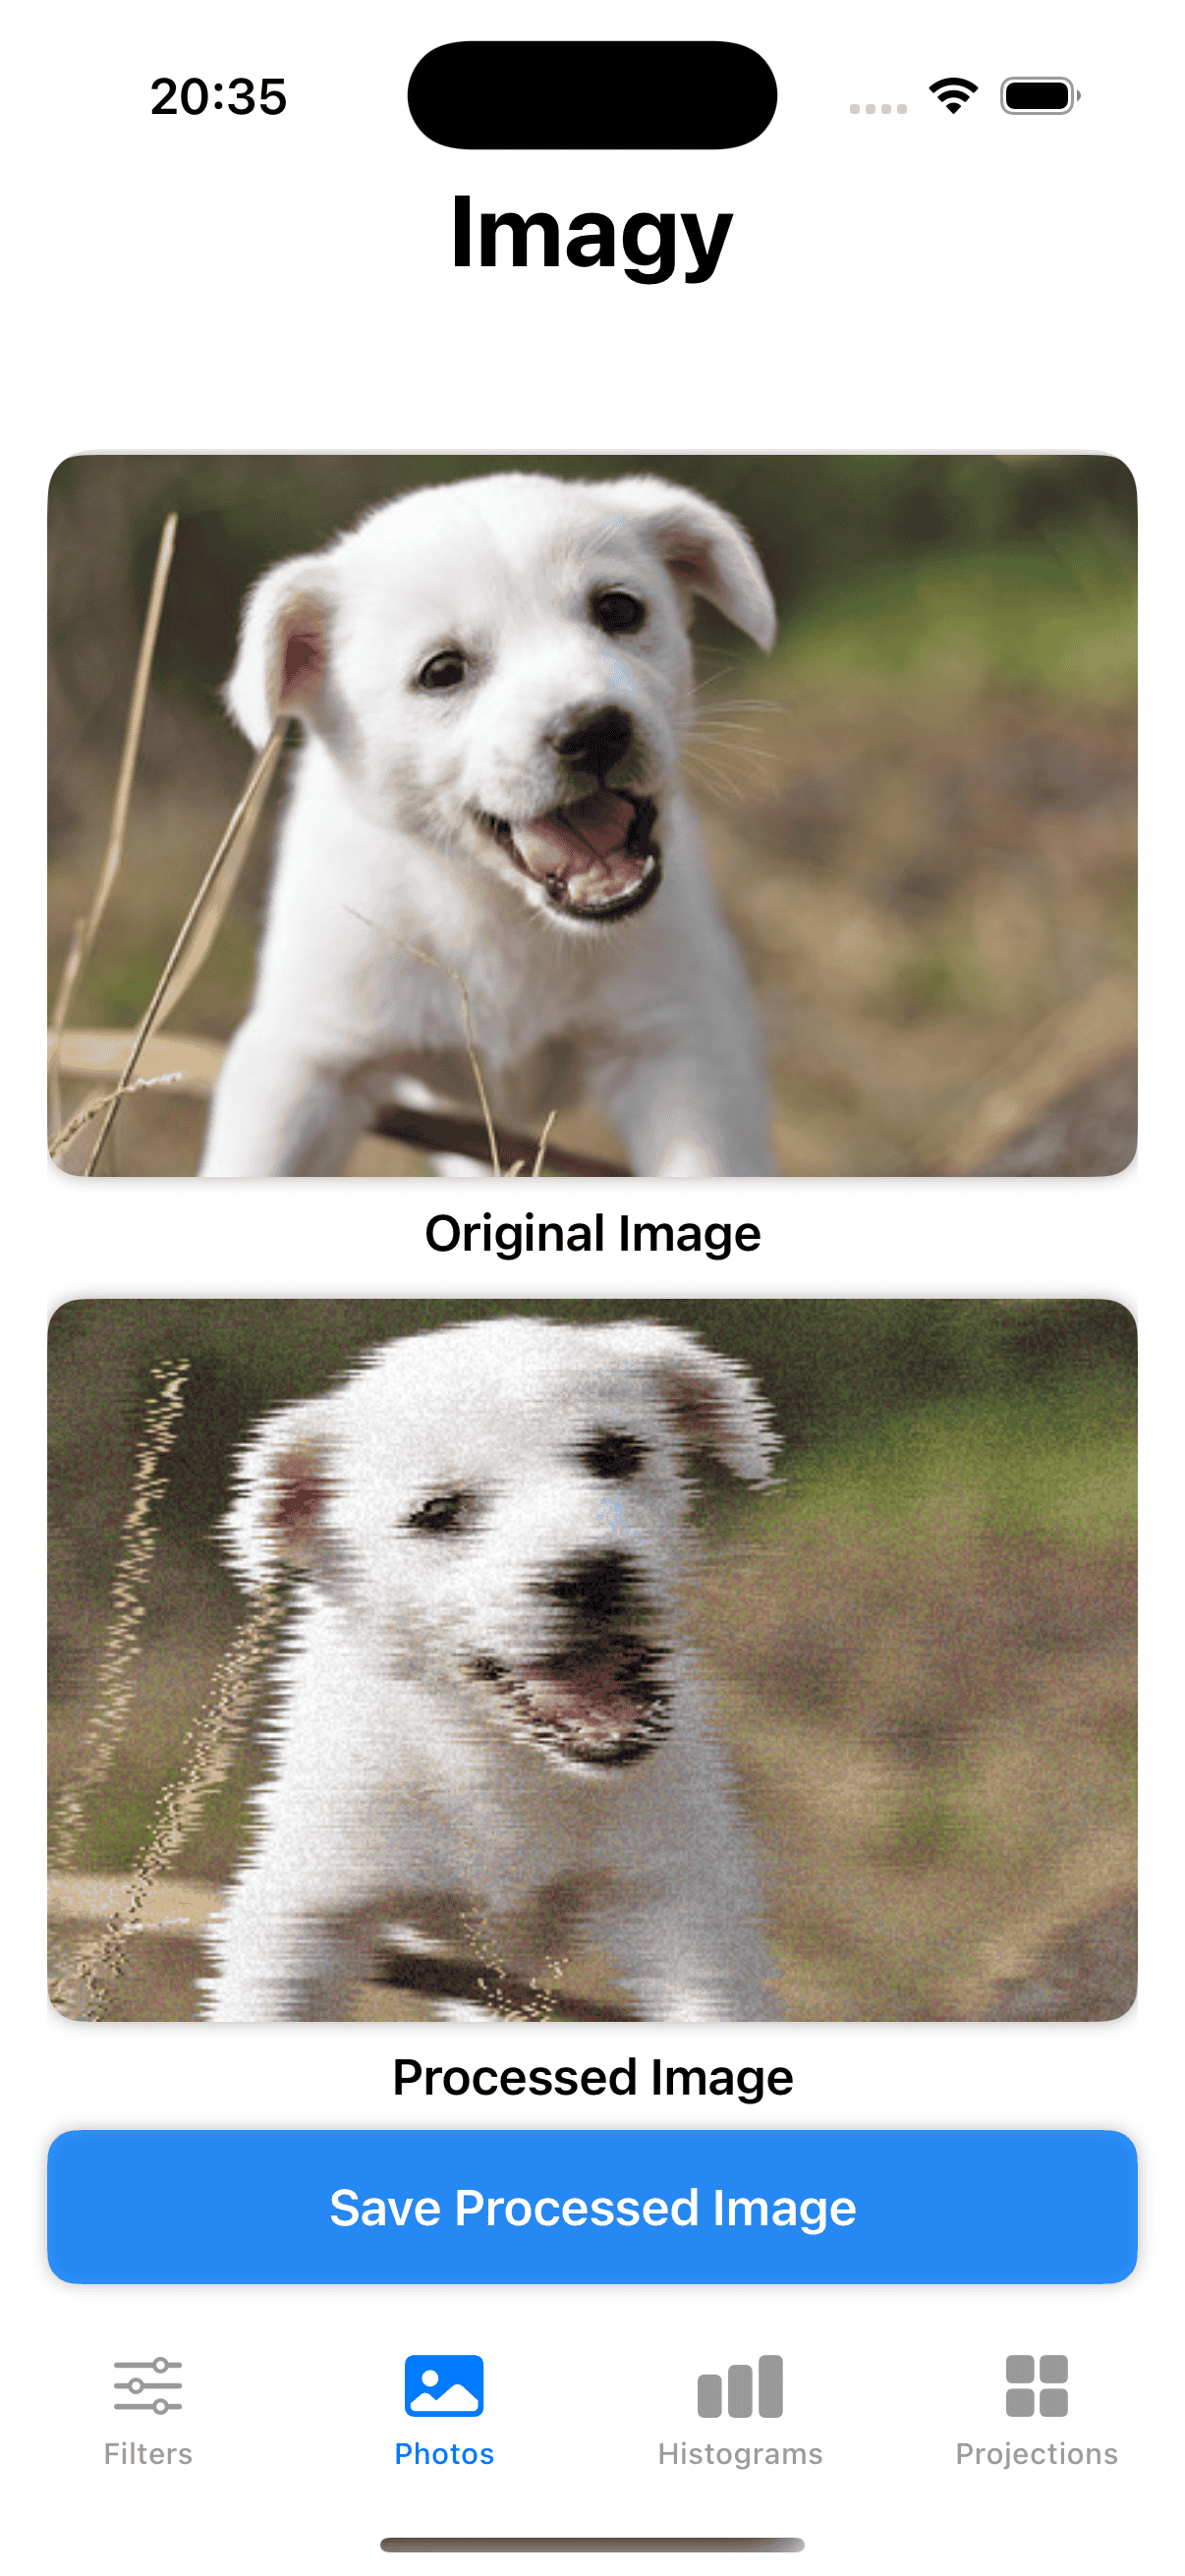
\includegraphics[width=\linewidth]{images/dog_glitch.png}
        \label{fig:dog_glitch}
    \end{subfigure}
    \begin{subfigure}{0.2\textwidth}
        \centering
        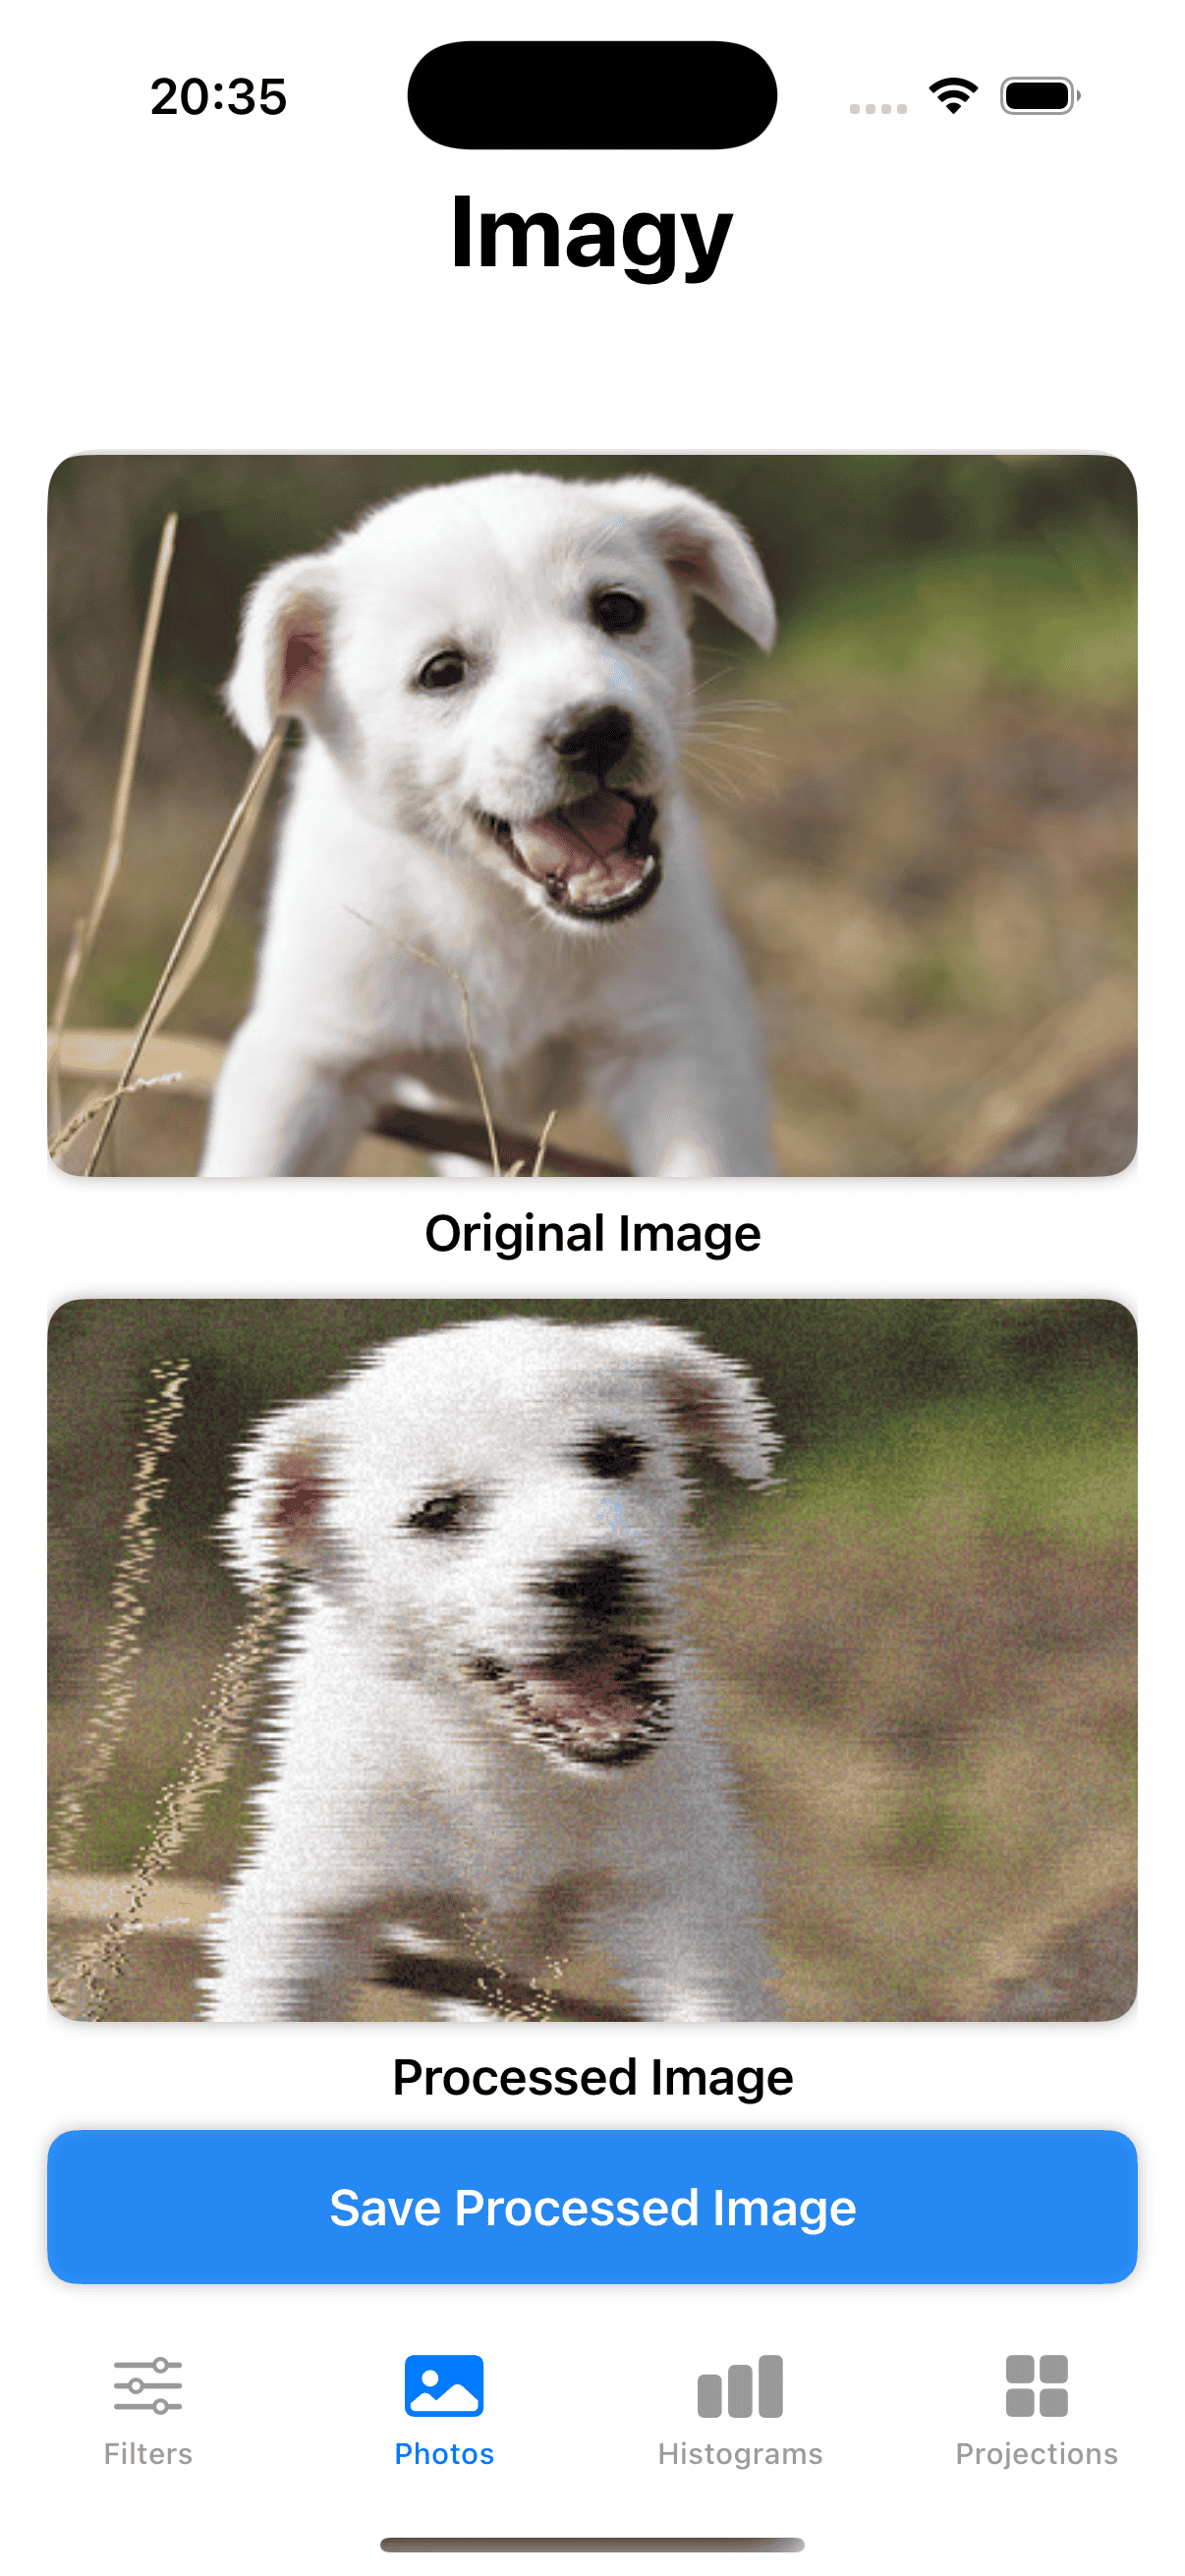
\includegraphics[width=\linewidth]{images/dog_glitch.png}
        \label{fig:dog_glitch}
    \end{subfigure}
    \caption{Glitch Blur filter - demonstracja. Tak jak wcześniej opisane, zdjęcia po przekształceniu sprawiają wrażenie jakby matryca je wyświetlająca była uszkodzona - stąd nazwa.}
    \label{fig:glitch}
\end{figure}

\subsection{Grayscale}

\begin{itemize}
    \item \texttt{static var name: String = "Grayscale"}
    \item Działanie - dla każdego z pikseli dodajemy wartości kanałów koloru i dzielimy przez 3. Każdy kanał koloru ustawiamy na tą wartość.
    \item Zastosowanie - tworzenie monochromatycznych obrazów.
\end{itemize}

\begin{figure}[H]
    \centering
    \begin{subfigure}{0.2\textwidth}
        \centering
        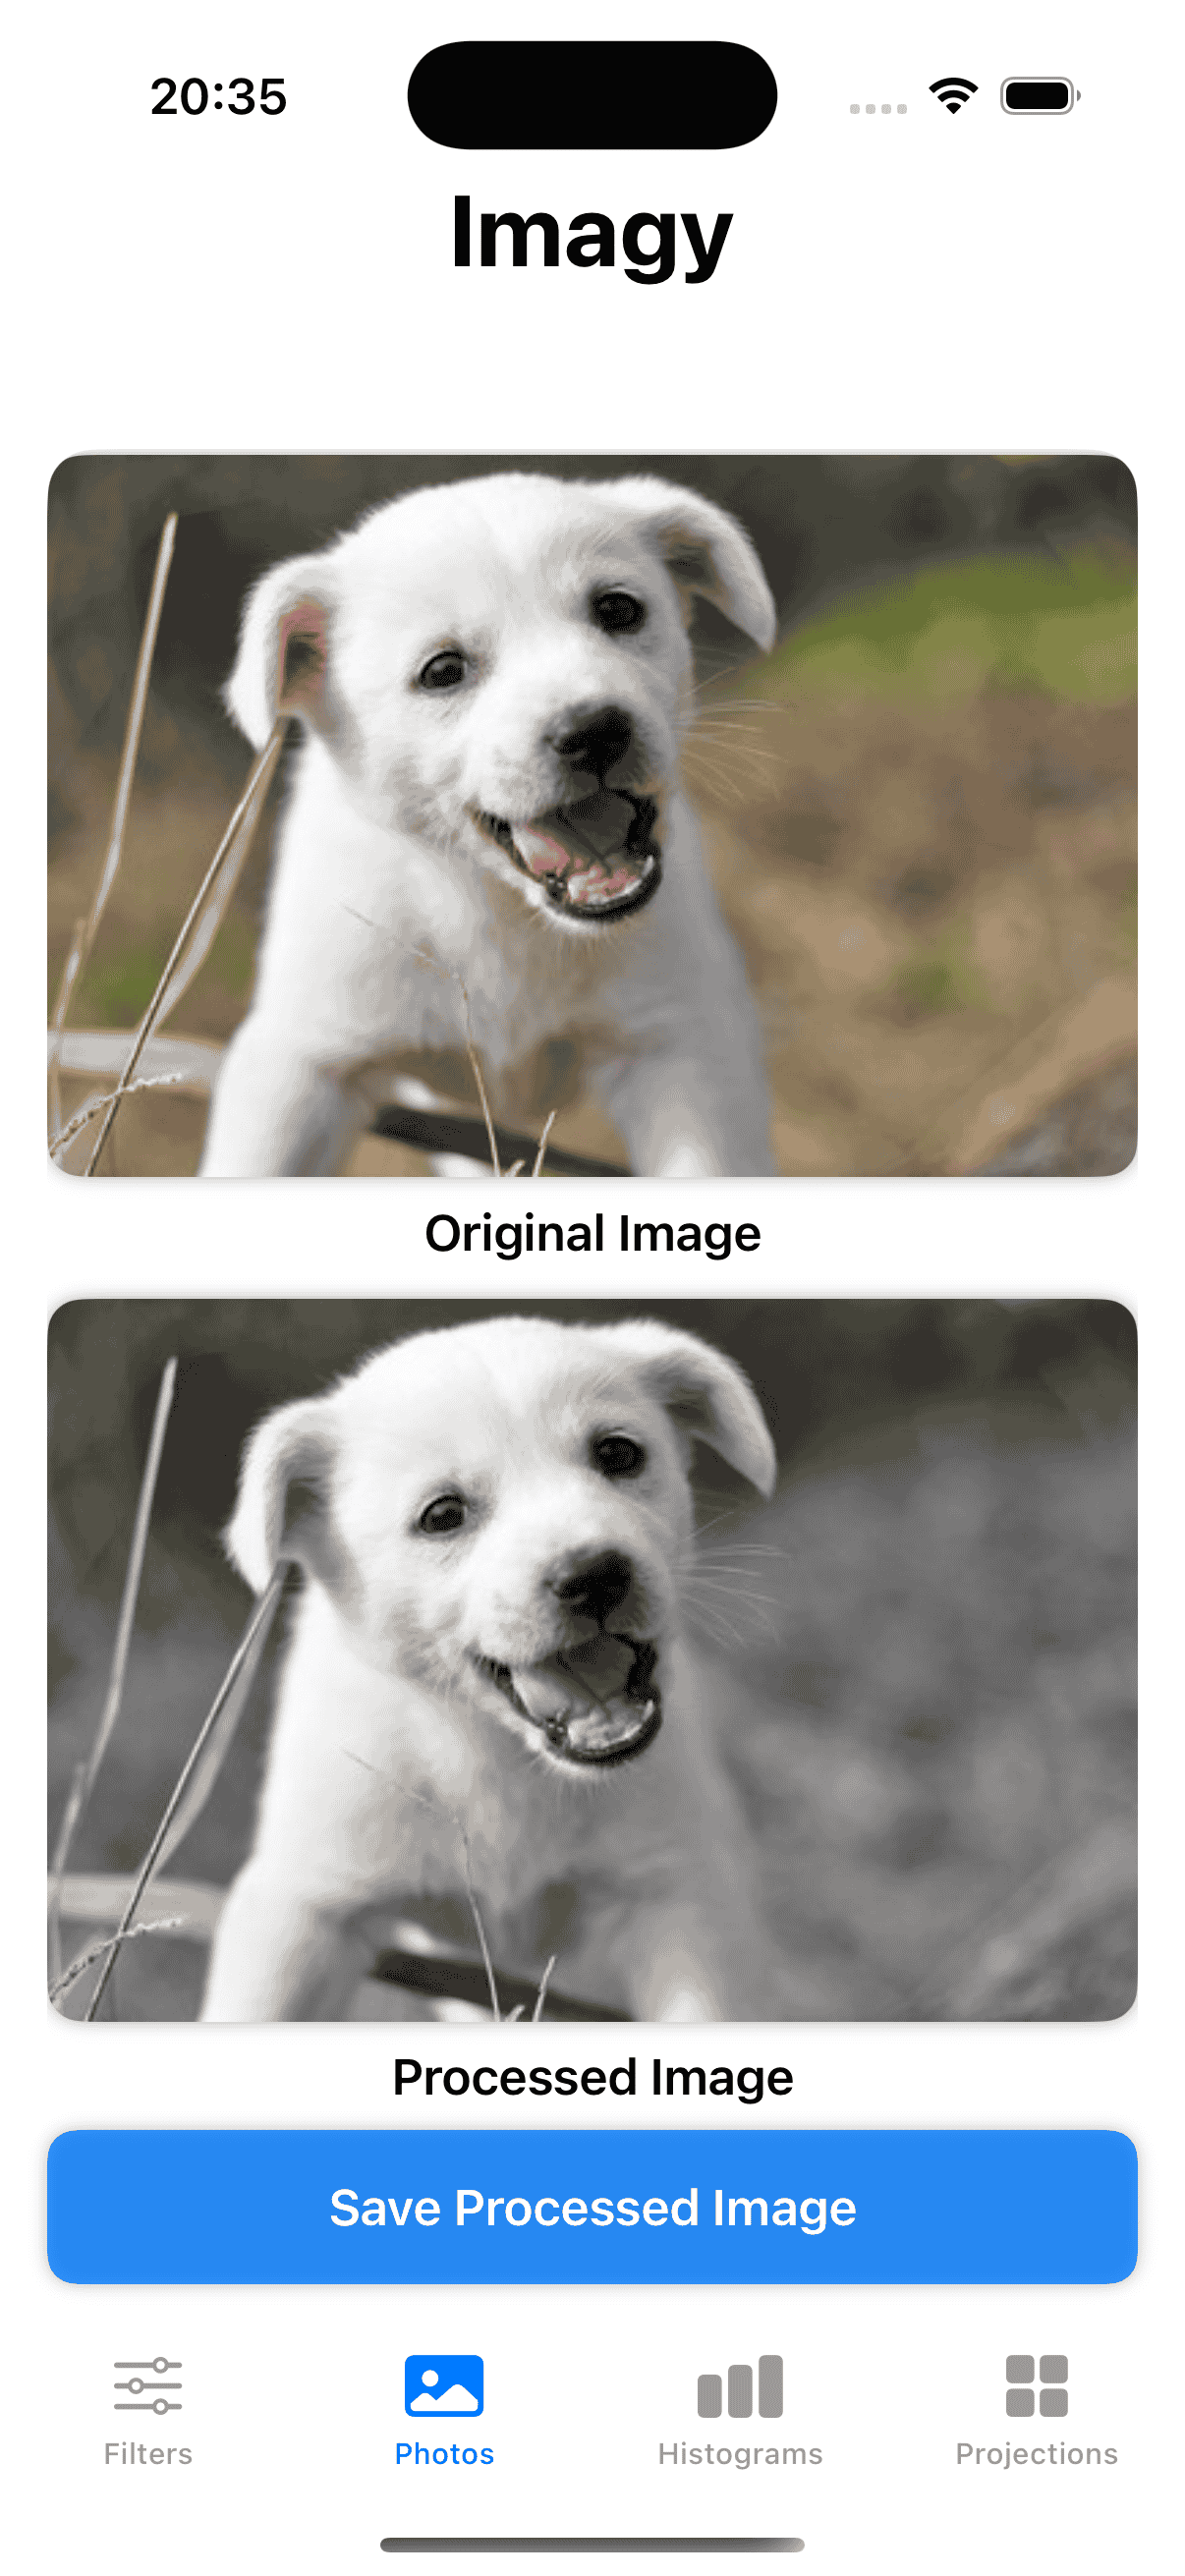
\includegraphics[width=\linewidth]{images/dog_gray.png}
        \label{fig:dog_gray}
    \end{subfigure}
    \begin{subfigure}{0.2\textwidth}
        \centering
        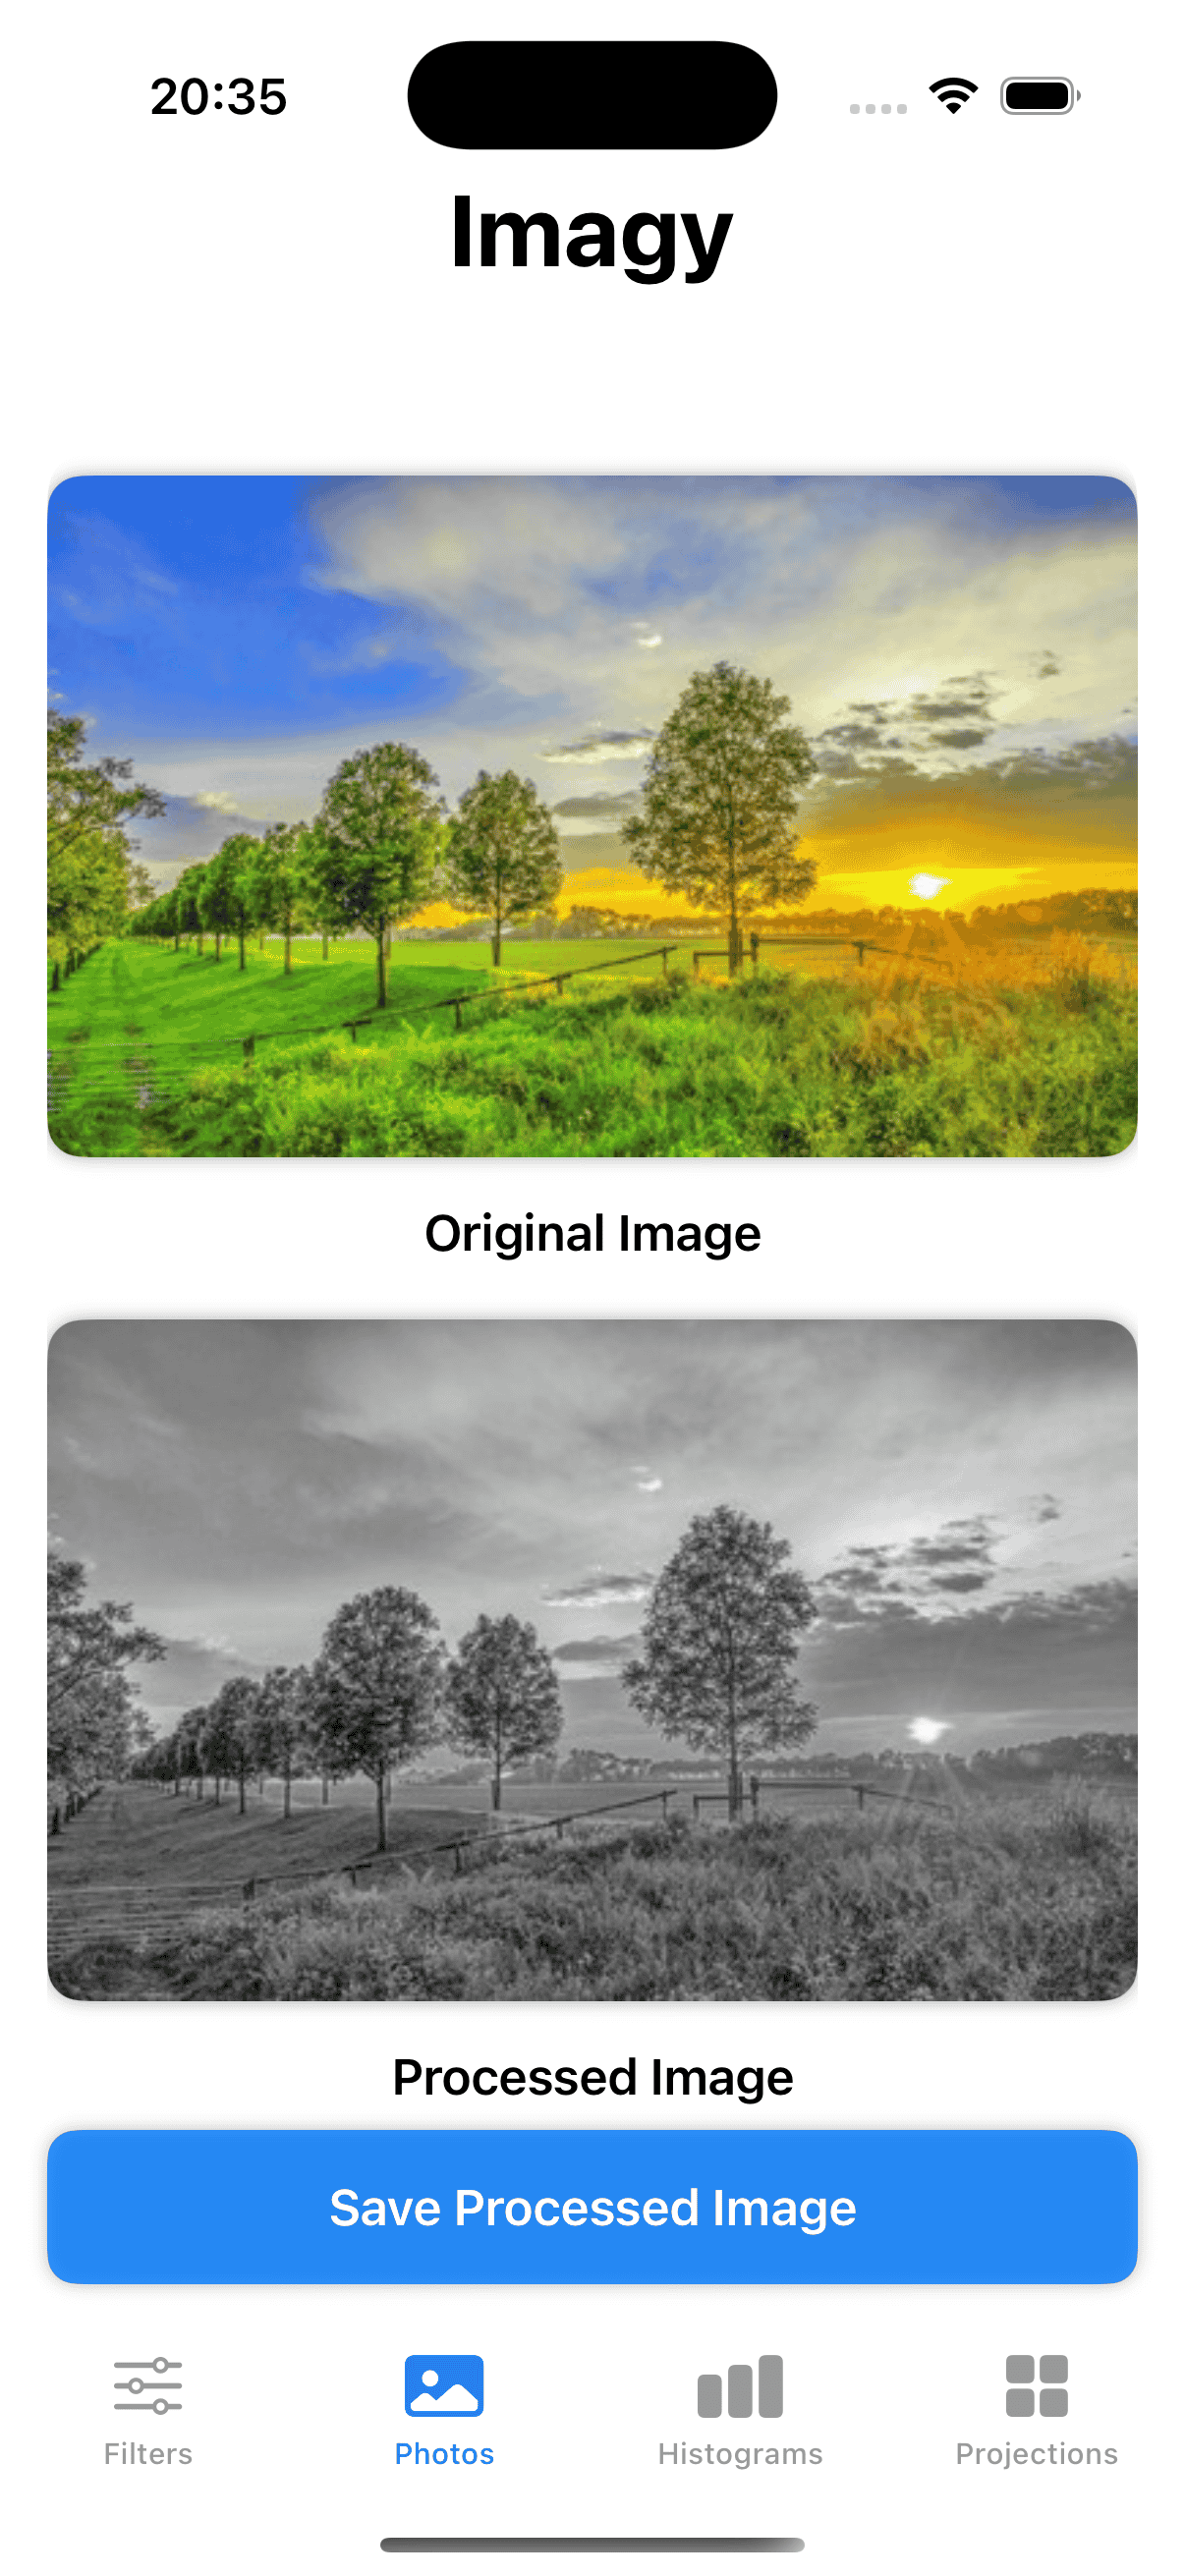
\includegraphics[width=\linewidth]{images/trees_gray.png}
        \label{fig:trees_gray}
    \end{subfigure}
    \caption{Grayscale Blur filter - demonstracja. Transformacja ze zdjęcia RGB robi zdjęcie czerno-białe, z zachowaniem jego jakości (choć w przypadku implementacji mojej aplikacji pod spodem dalej jest reprezentowane przez zdjęcie RGBA, po prostu każdy kanał kolory ma tą samą wartość dla konkretnego piksela.)}
    \label{fig:glitch}
\end{figure}

\subsection{Mosaic}

\begin{itemize}
    \item \texttt{static var name: String = "Mosaic"}
    \item \texttt{ blockSize: Int} - rozmiar bloku. Defaultowo $10$, pobierany z widoku GUI ograniczony do wartości z zakresu $2-15$ z krokiem $1$.
    \item Działanie - przesuwamy ustalonej wartości blok (ze stride jako pełny blok, tj tworzymy z obrazu rozbicie na małe bloki ustalonej wielkości), piksele wewnątrz każdego bloku ustawiamy (dla każdego z kanałów oddzielnie) na średnią wartość tego kanału wewnątrz bloku.
    \item Zastosowanie - cenzura, efekty artystyczne, stylizacja.
\end{itemize}

\begin{figure}[H]
    \centering
    \begin{subfigure}{0.2\textwidth}
        \centering
        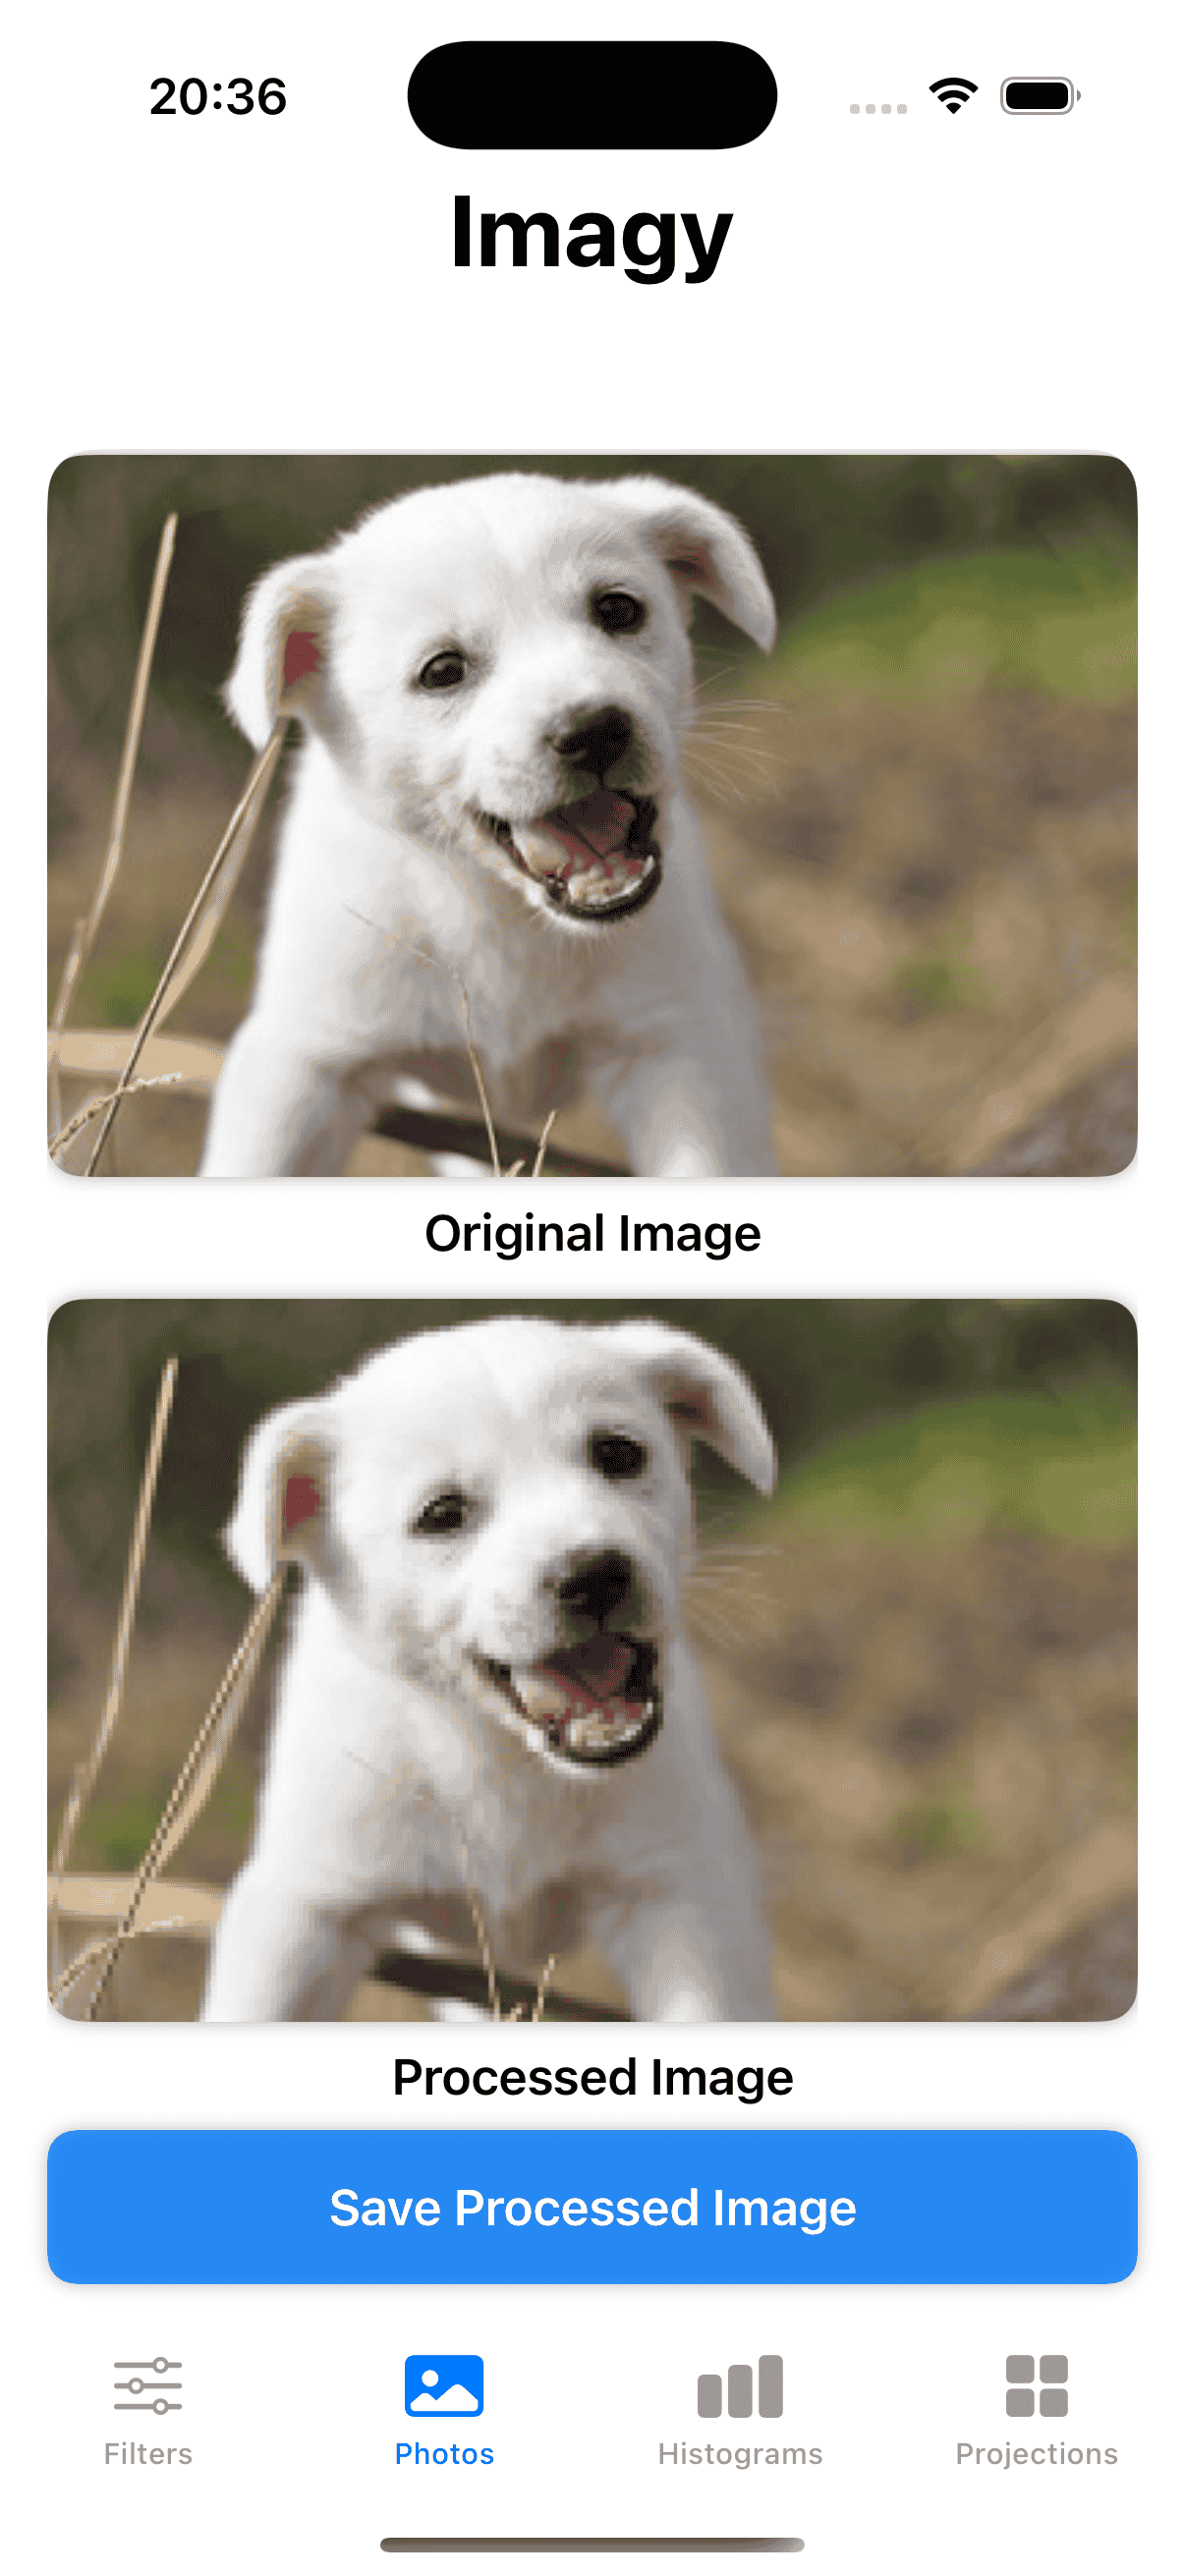
\includegraphics[width=\linewidth]{images/dog_mosaic_2.png}
        \caption{blockSize=2}
        \label{fig:dog_mosaic_2}
    \end{subfigure}
    \hfill
    \begin{subfigure}{0.2\textwidth}
        \centering
        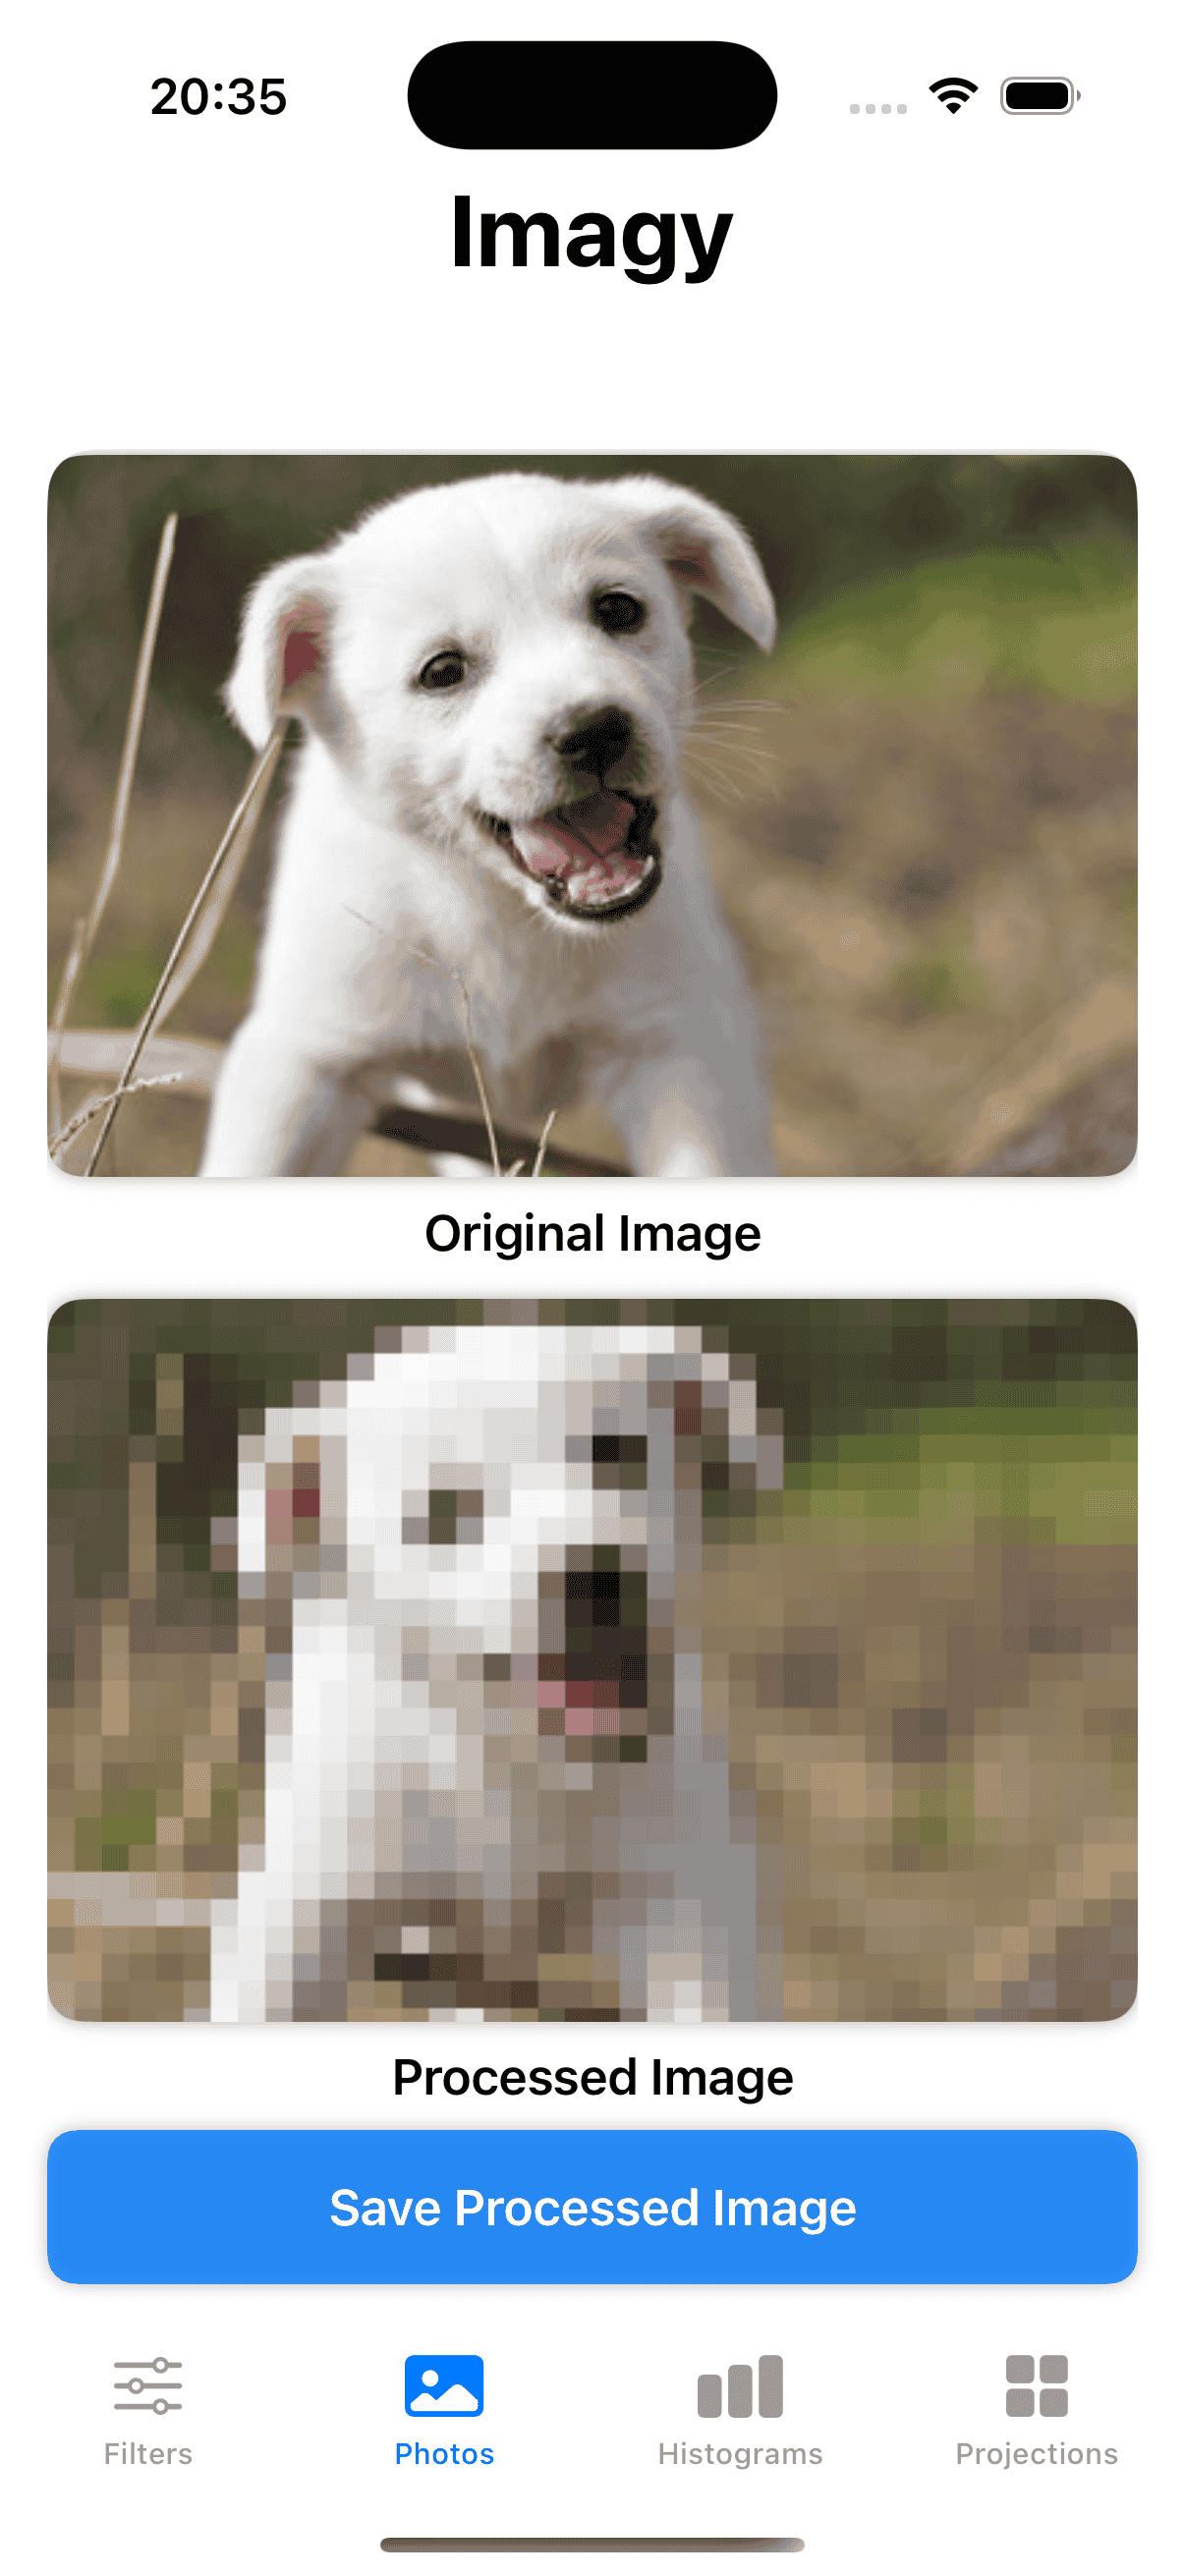
\includegraphics[width=\linewidth]{images/dog_mosaic_10.png}
        \caption{blockSize=10}
        \label{fig:dog_mosaic_10}
    \end{subfigure}
    \hfill
    \begin{subfigure}{0.2\textwidth}
        \centering
        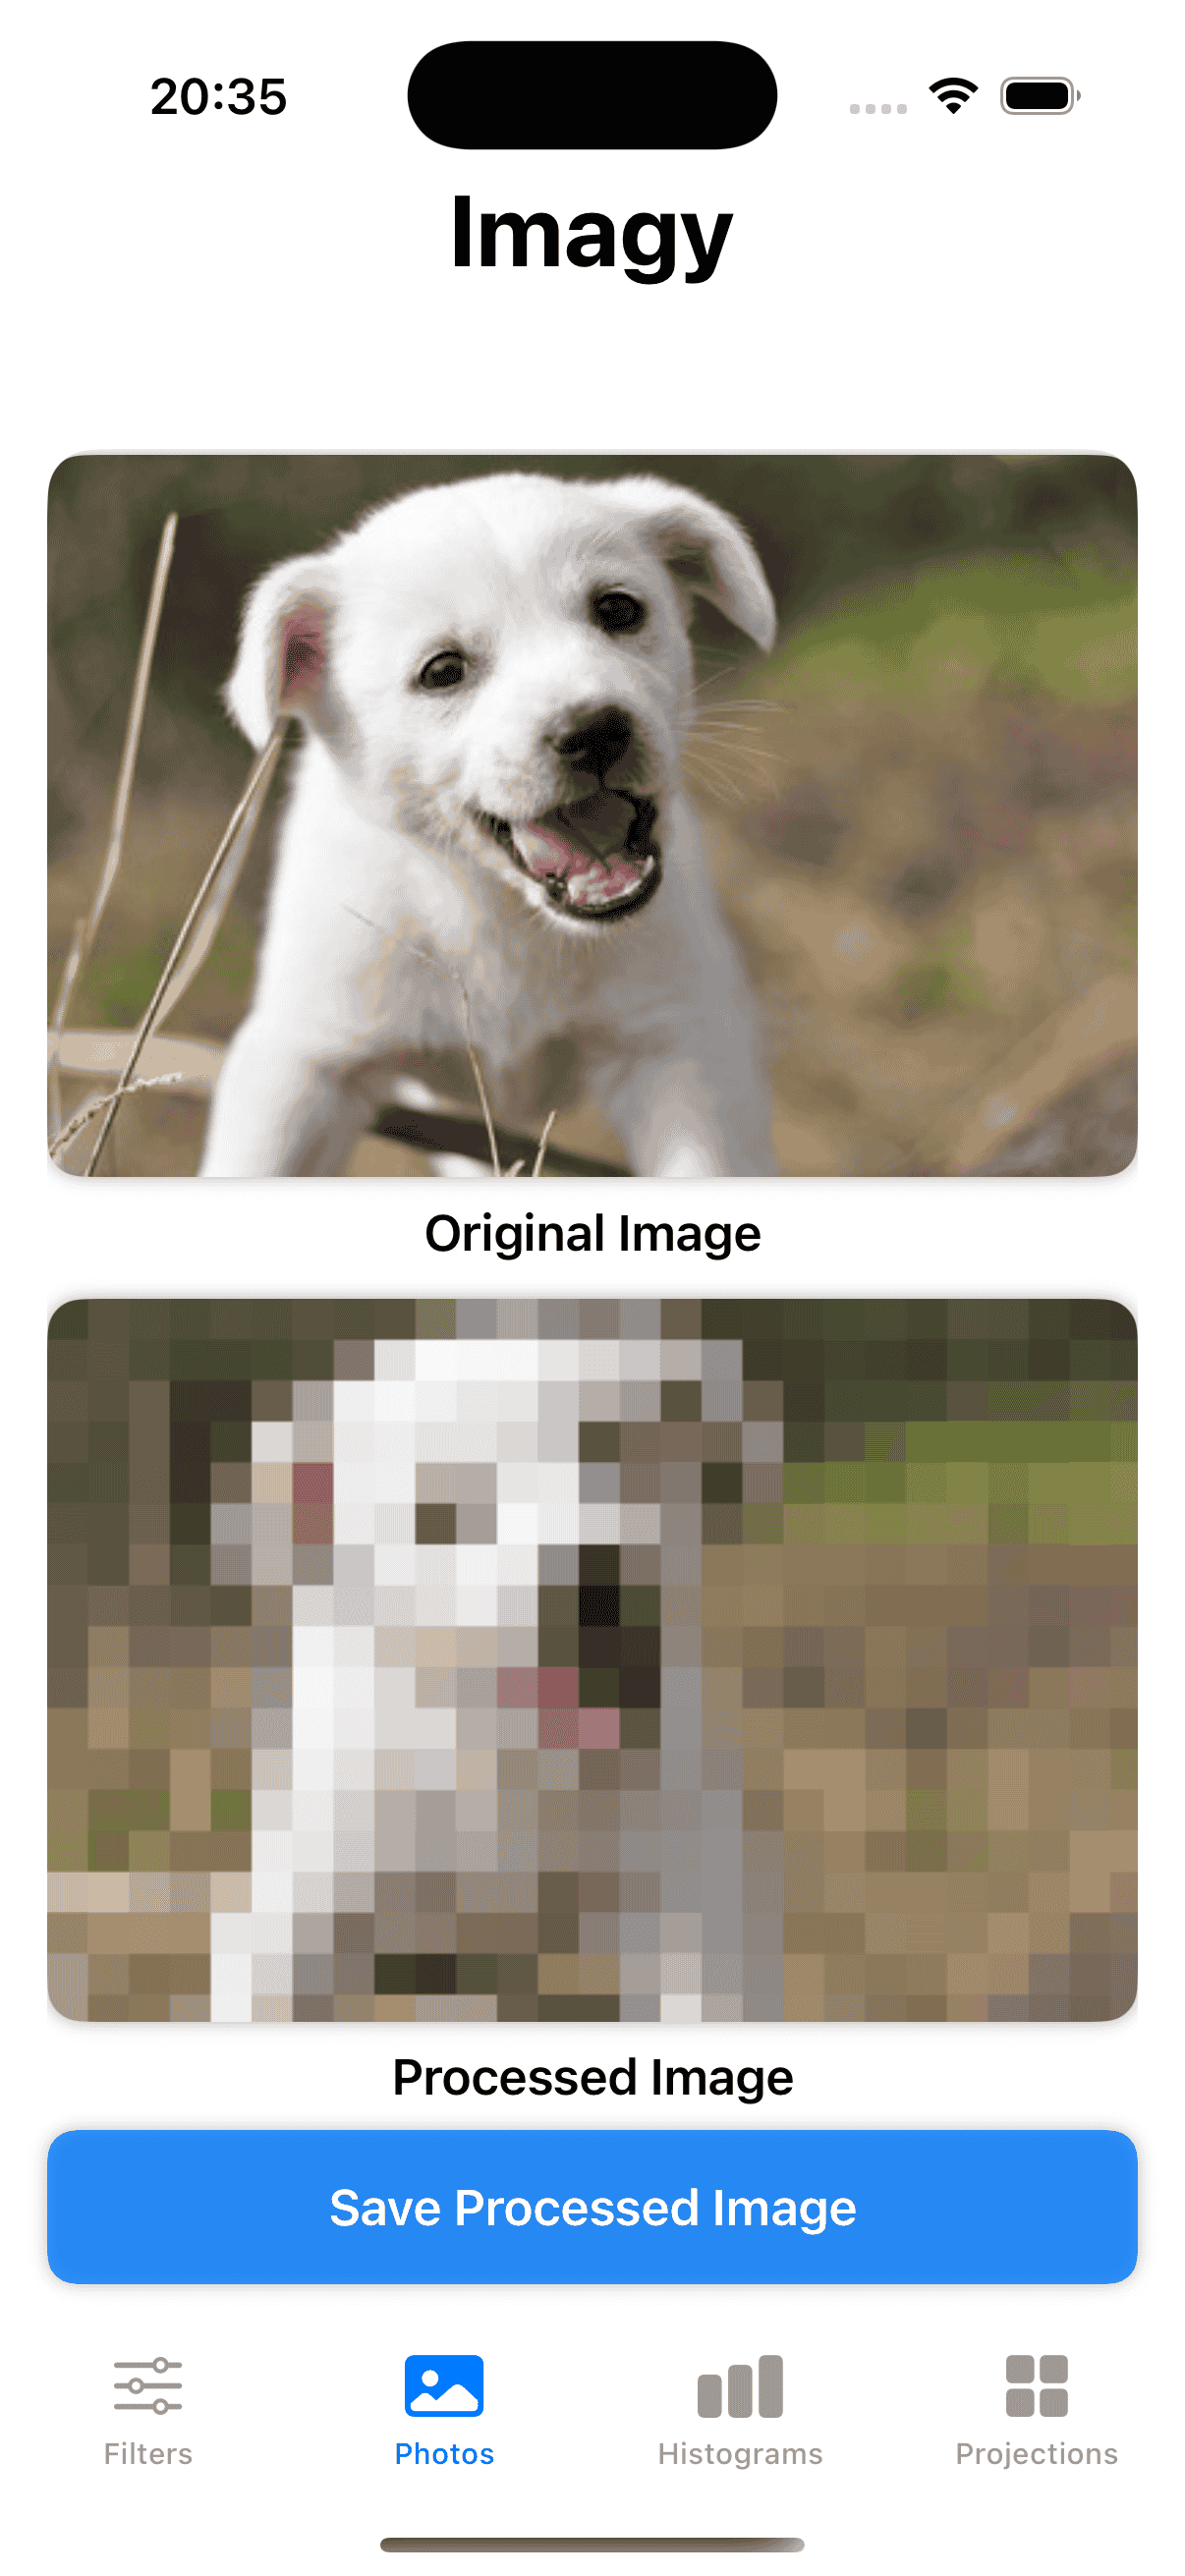
\includegraphics[width=\linewidth]{images/dog_mosaic_15.png}
        \caption{blockSize=15}
        \label{fig:dog_mosaic_15}
    \end{subfigure}
    \caption{Mosaic filter - demonstracja. Większy blockSize powoduje coraz bardziej widoczne bloki tego samego koloru na zdjęciu. W pewnym sensie można go interpretować jako rzut na matrycę o gorszej rozdzielczości. blockSize=2 prezentuje to najmniej drastycznie, dopiero przyjrzenie się ździbłom trawy ujawnia w sposób oczywisty że mamy tu doczynienia z przefiltrowanym zdjęciem a nie wykonanym przez aparat o gorszej rozdzielczości.}
    \label{fig:mosaic}
\end{figure}

\subsection{Negative}

\begin{itemize}
    \item \texttt{static var name: String = "Negative"}
    \item Działanie - dla każdego z pikseli (każdego z kanałów oddzielnie) ustawiamy wartość $255 - x$ gdzie $x$ to wartość poprzednia (oryginalna).
    \item Zastosowanie - digitalizacja dokumentów, preprocessing do Computer Vision
\end{itemize}

\begin{figure}[H]
    \centering
    \begin{subfigure}{0.2\textwidth}
        \centering
        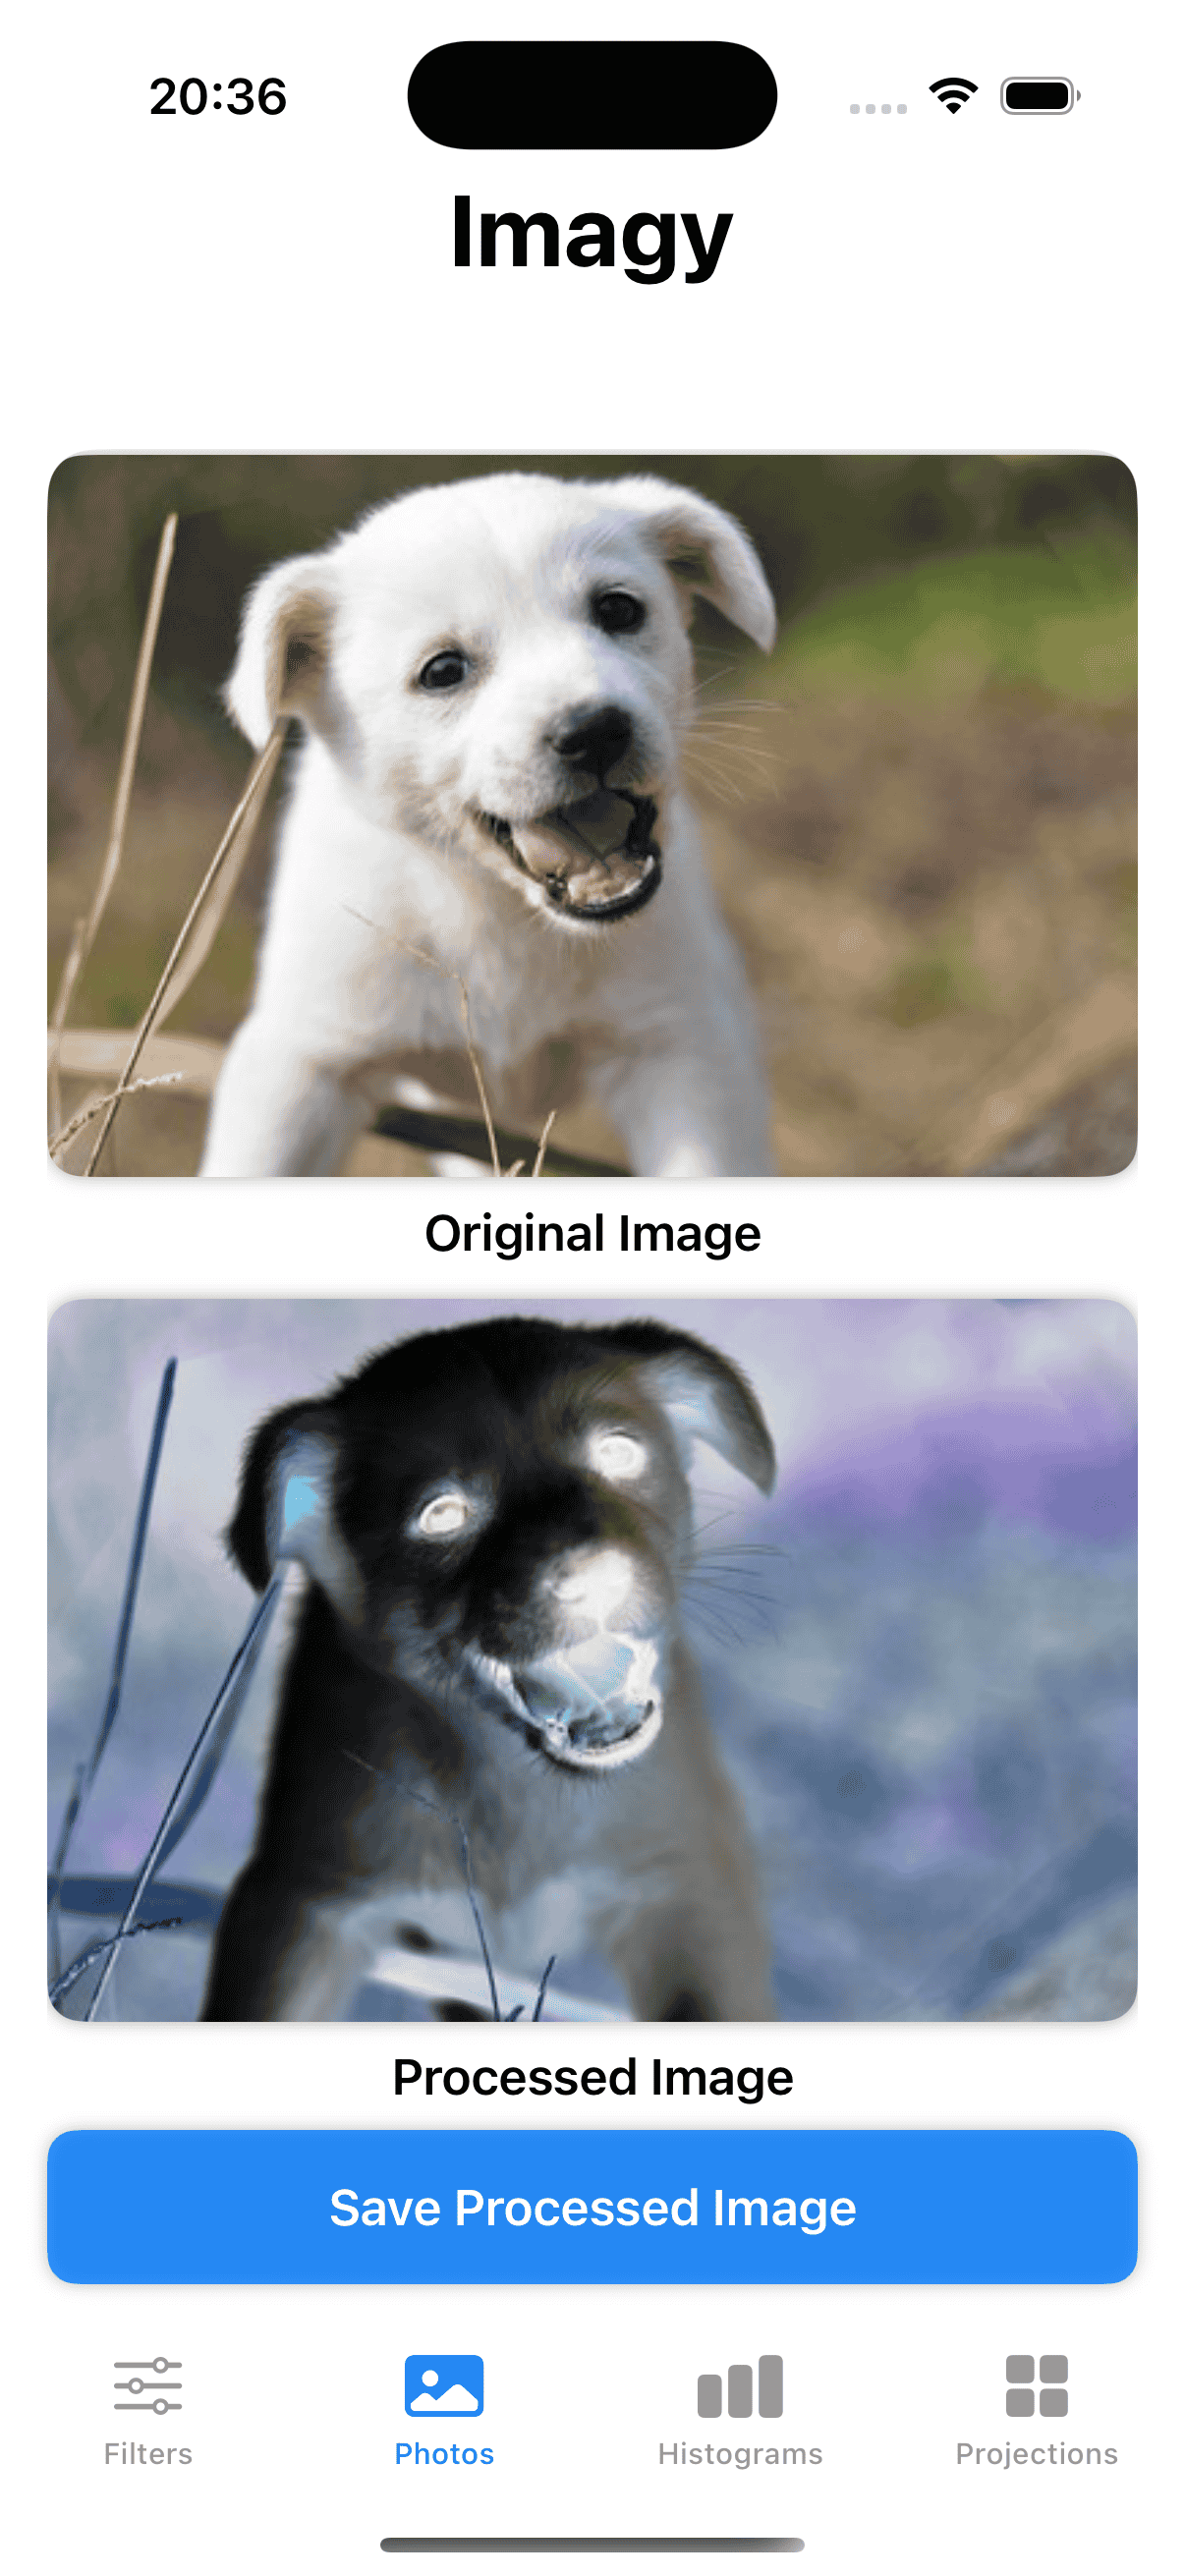
\includegraphics[width=\linewidth]{images/dog_negative.png}
        \label{fig:dog_negative}
    \end{subfigure}
    \begin{subfigure}{0.2\textwidth}
        \centering
        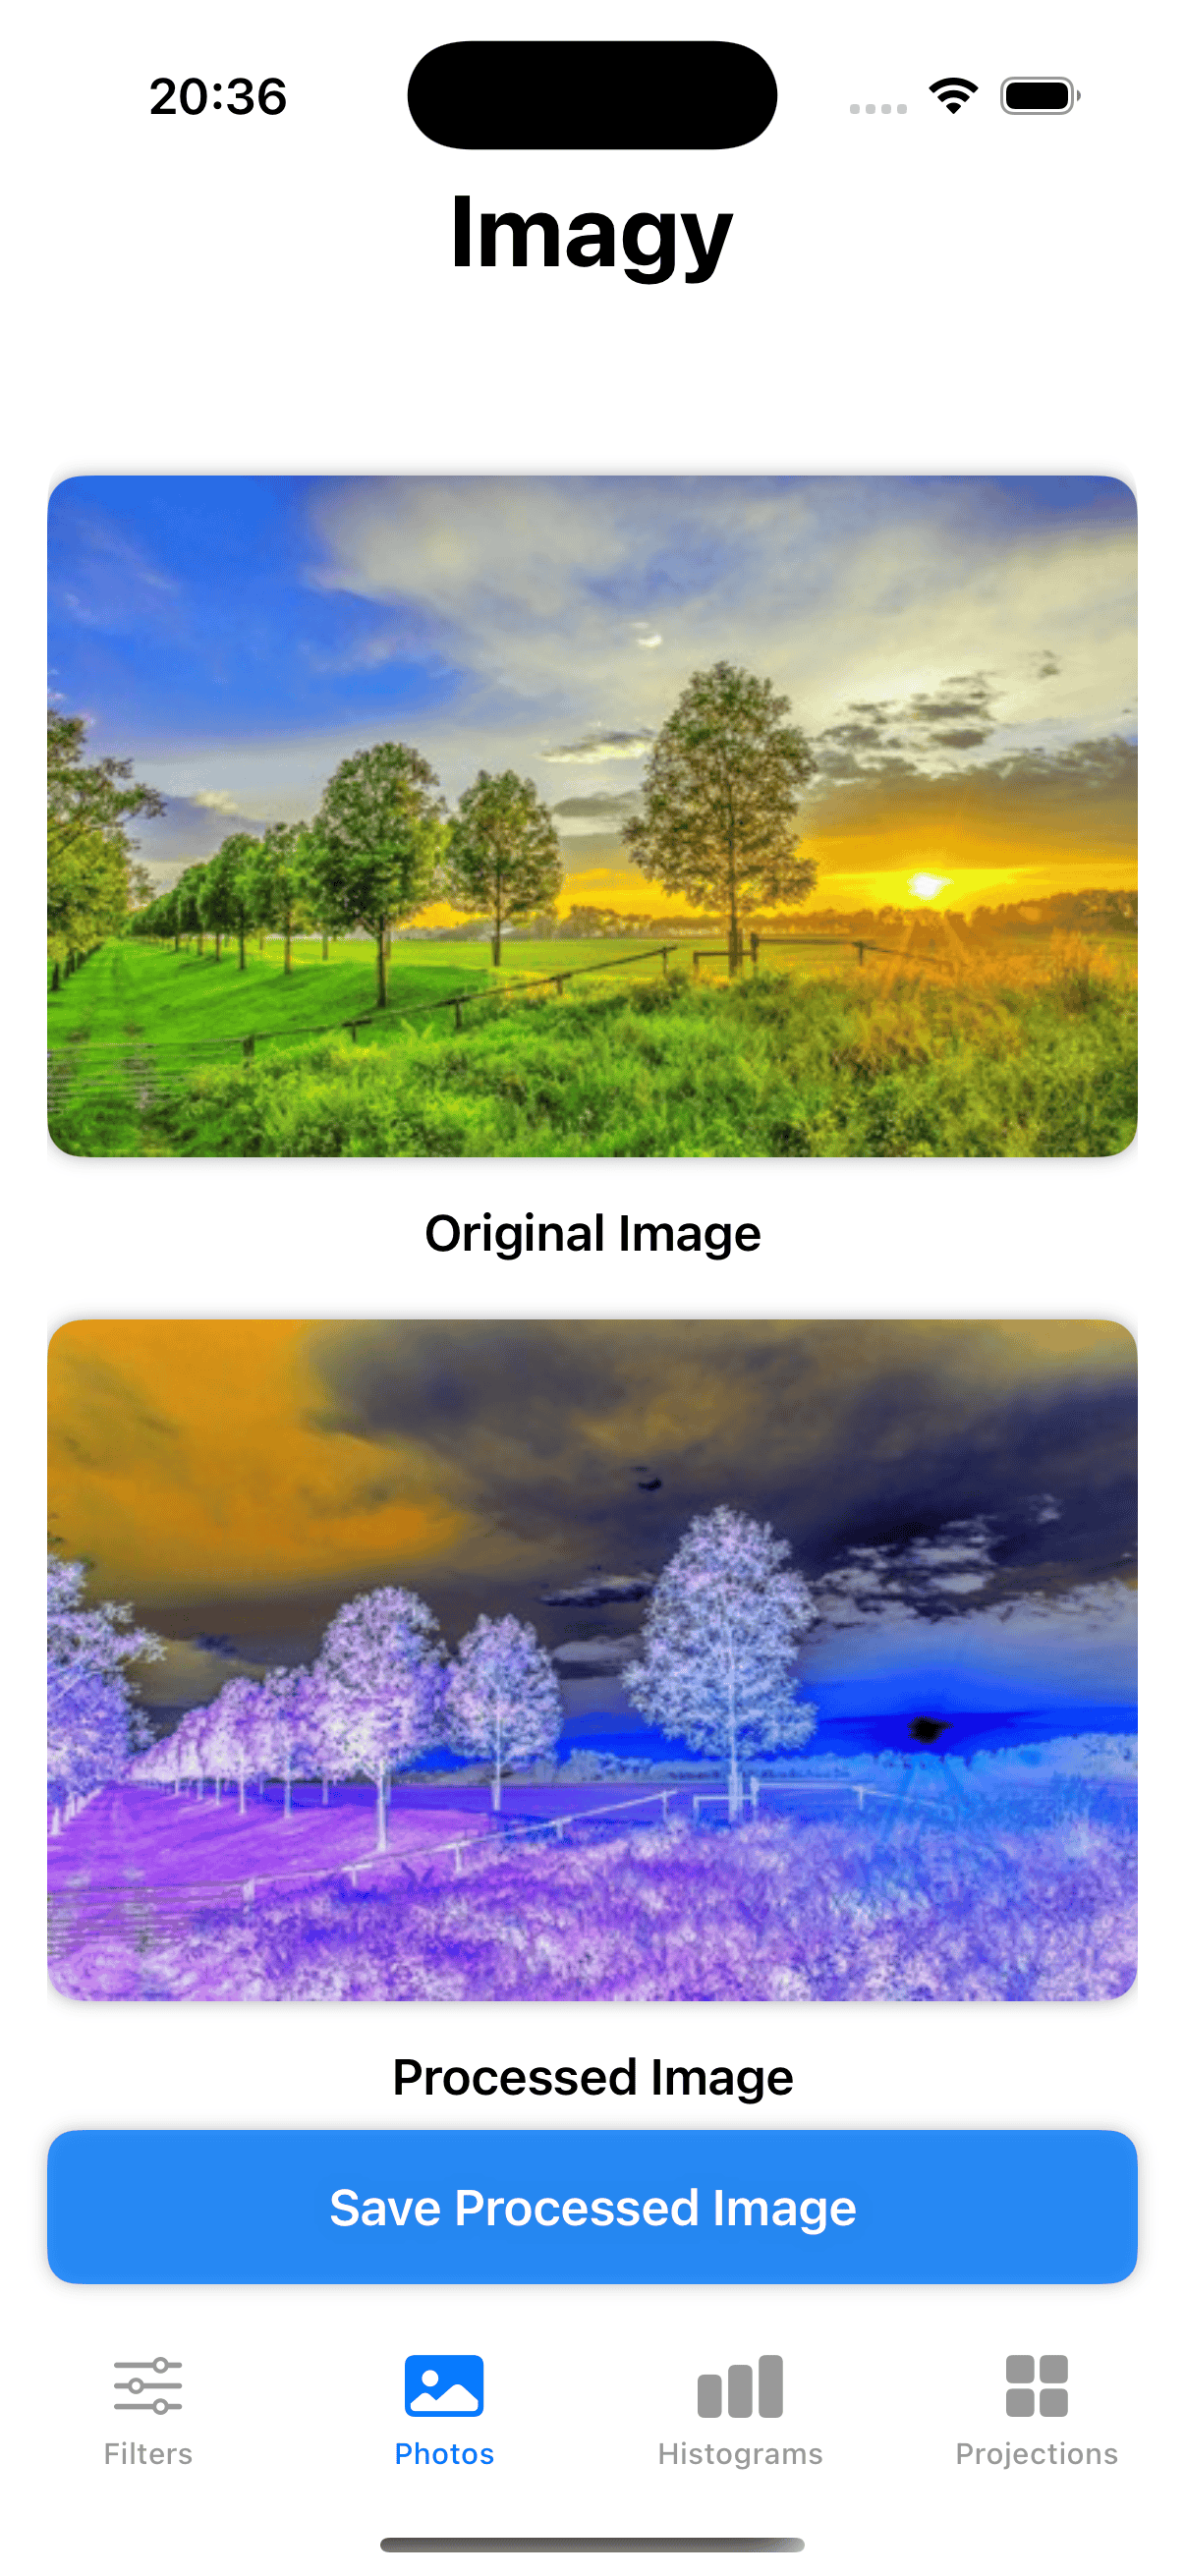
\includegraphics[width=\linewidth]{images/trees_negative.png}
        \label{fig:trees_negative}
    \end{subfigure}
    \caption{Nagative filter - demonstracja. Odwrócone kolory prowadzą do zdjęć dla ludzi bardzo nienaturalnych, jednak potrafią podkreślić cechy normalnie ukryte, stąd jego popularność w niektórych algorytmach Computer Vision.}
    \label{fig:glitch}
\end{figure}

\begin{figure}[H]
    \centering
    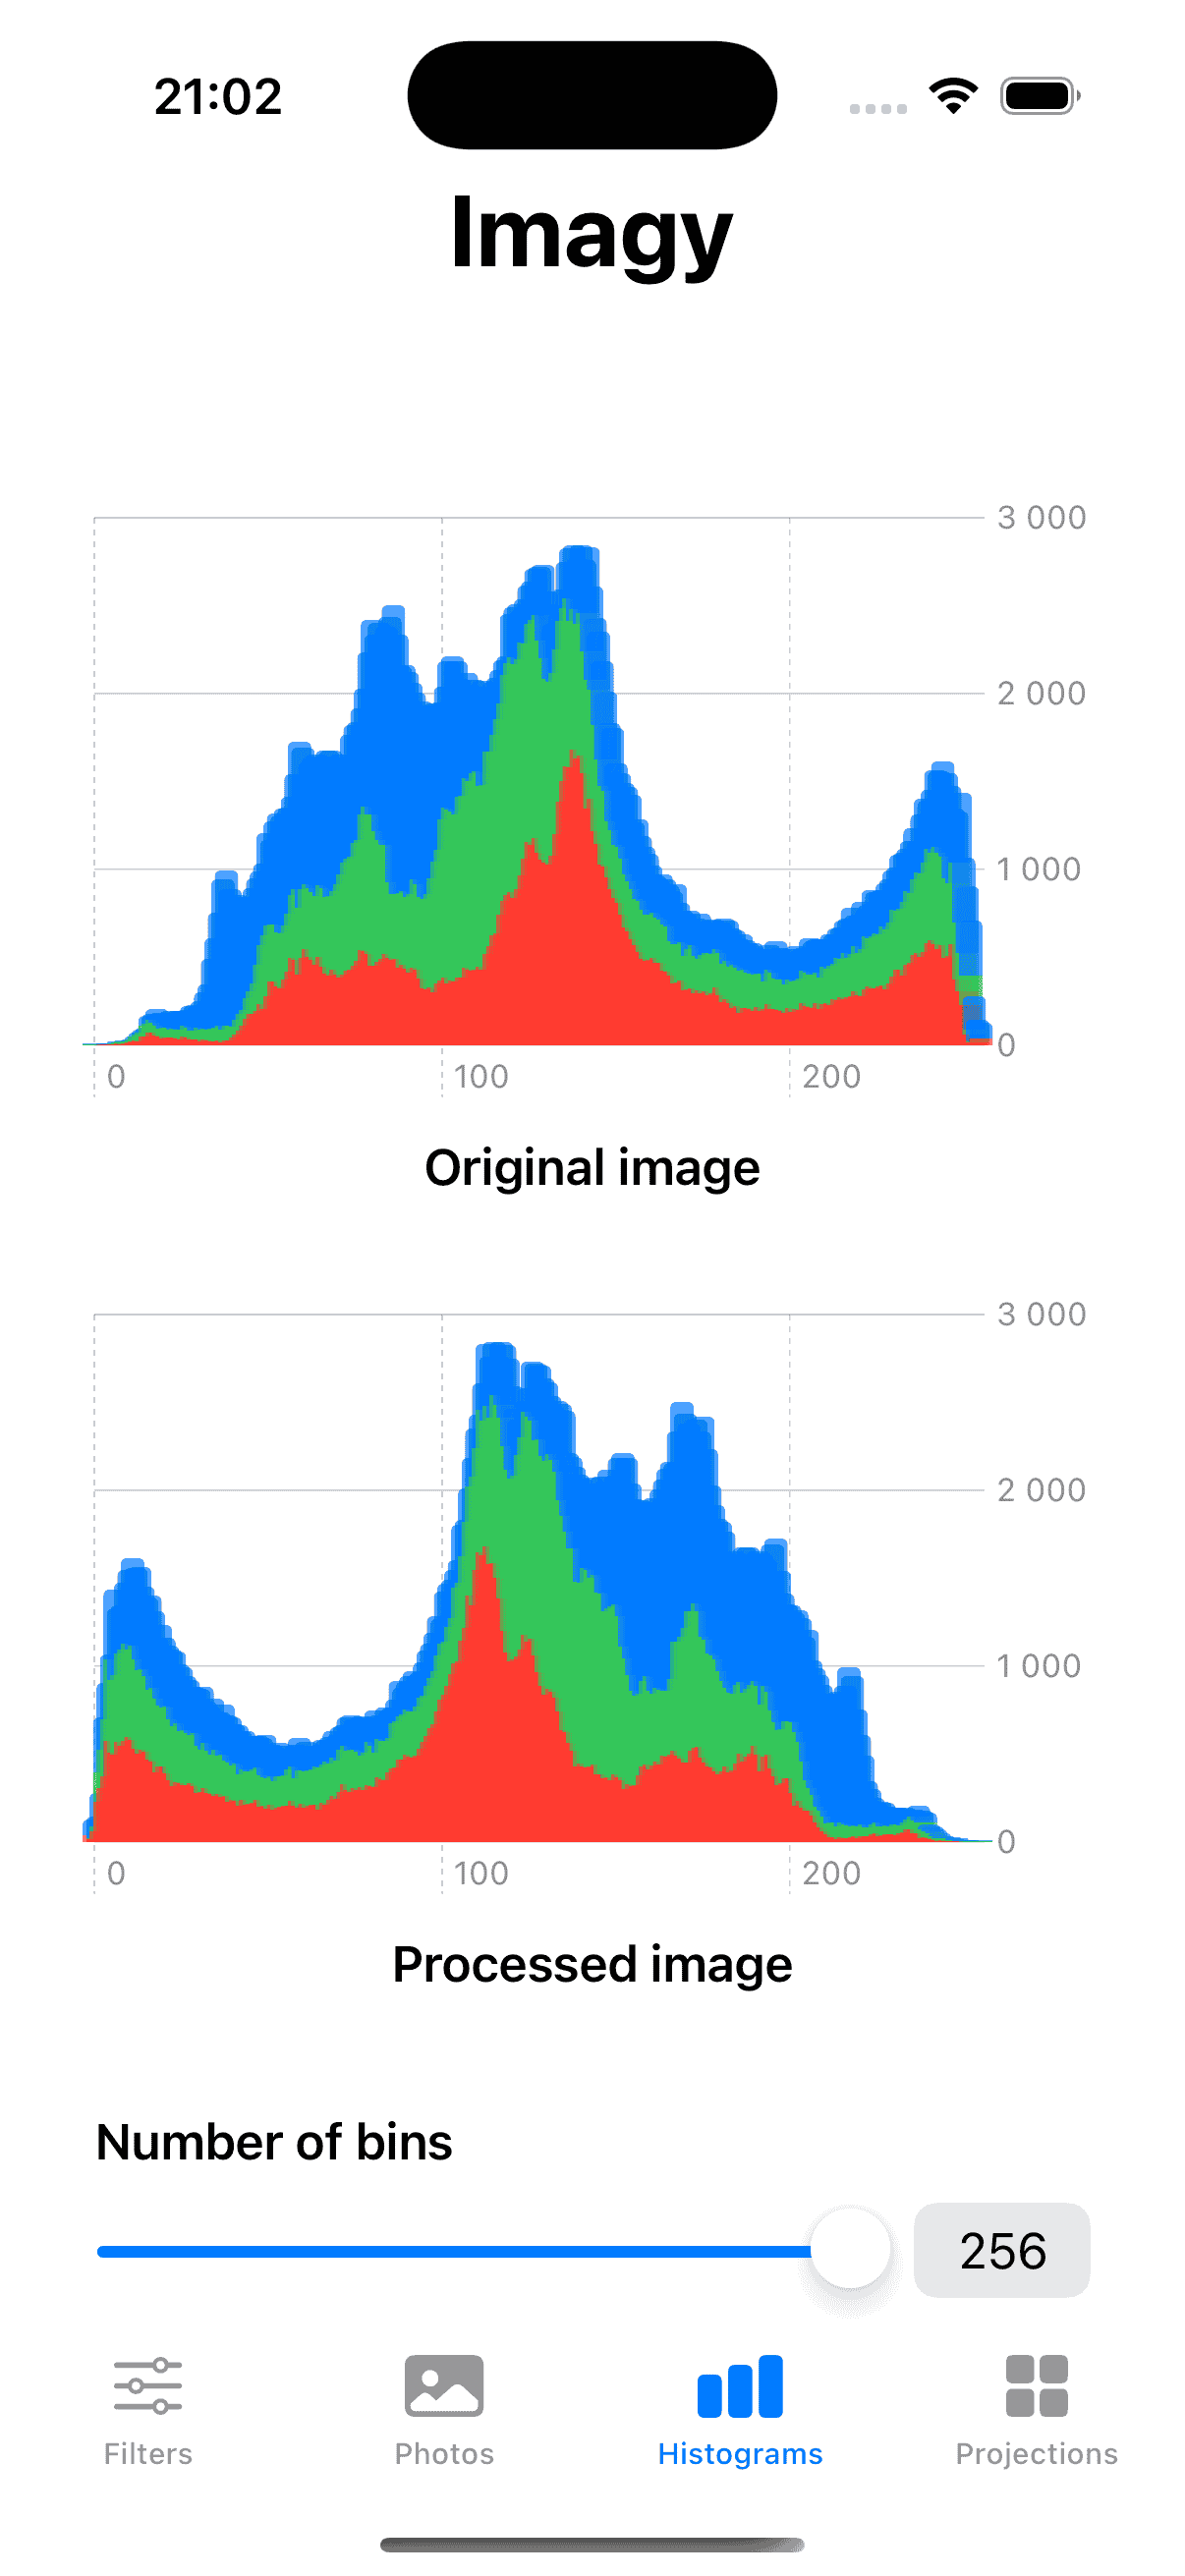
\includegraphics[width=0.25\linewidth]{images/dog_negative_histogram.png}
    \caption{Histogram for dog's negative filter.}
    \label{fig:dog_negative_histogram}
\end{figure}

\subsection{Posterize}

\begin{itemize}
    \item \texttt{static var name: String = "Posterize"}
    \item \texttt{ levels: Int } - rozmiar bloku. Defaultowo $4$, pobierany z widoku GUI ograniczony do wartości z zakresu $2-128$ z krokiem $2$. Większość źródeł wspominających o filtrze nie zaleca więcej niż 32 poziomów, tutaj ograniczenie podniesione w celach demonstracyjnych.
    \item Każdy piksel, każdy kanał wyliczany zgodnie ze wzorem:
          $$
              N = \frac{255}{P} \times \left\lfloor \frac{C \times P}{255} \right\rfloor
          $$
          Gdzie $N$ - nowa wartość, $P$ - liczba poziomów, $C$ - oryginalna wartość.
    \item Zastosowanie - efekty artystyczne, segmentacja, gry komputerowe - filtr nadaje obrazowi bardziej uproszczony styl, ponieważ redukuje liczbę dostępnych poziomów jasności.
\end{itemize}

\begin{figure}[H]
    \centering
    \begin{subfigure}{0.2\textwidth}
        \centering
        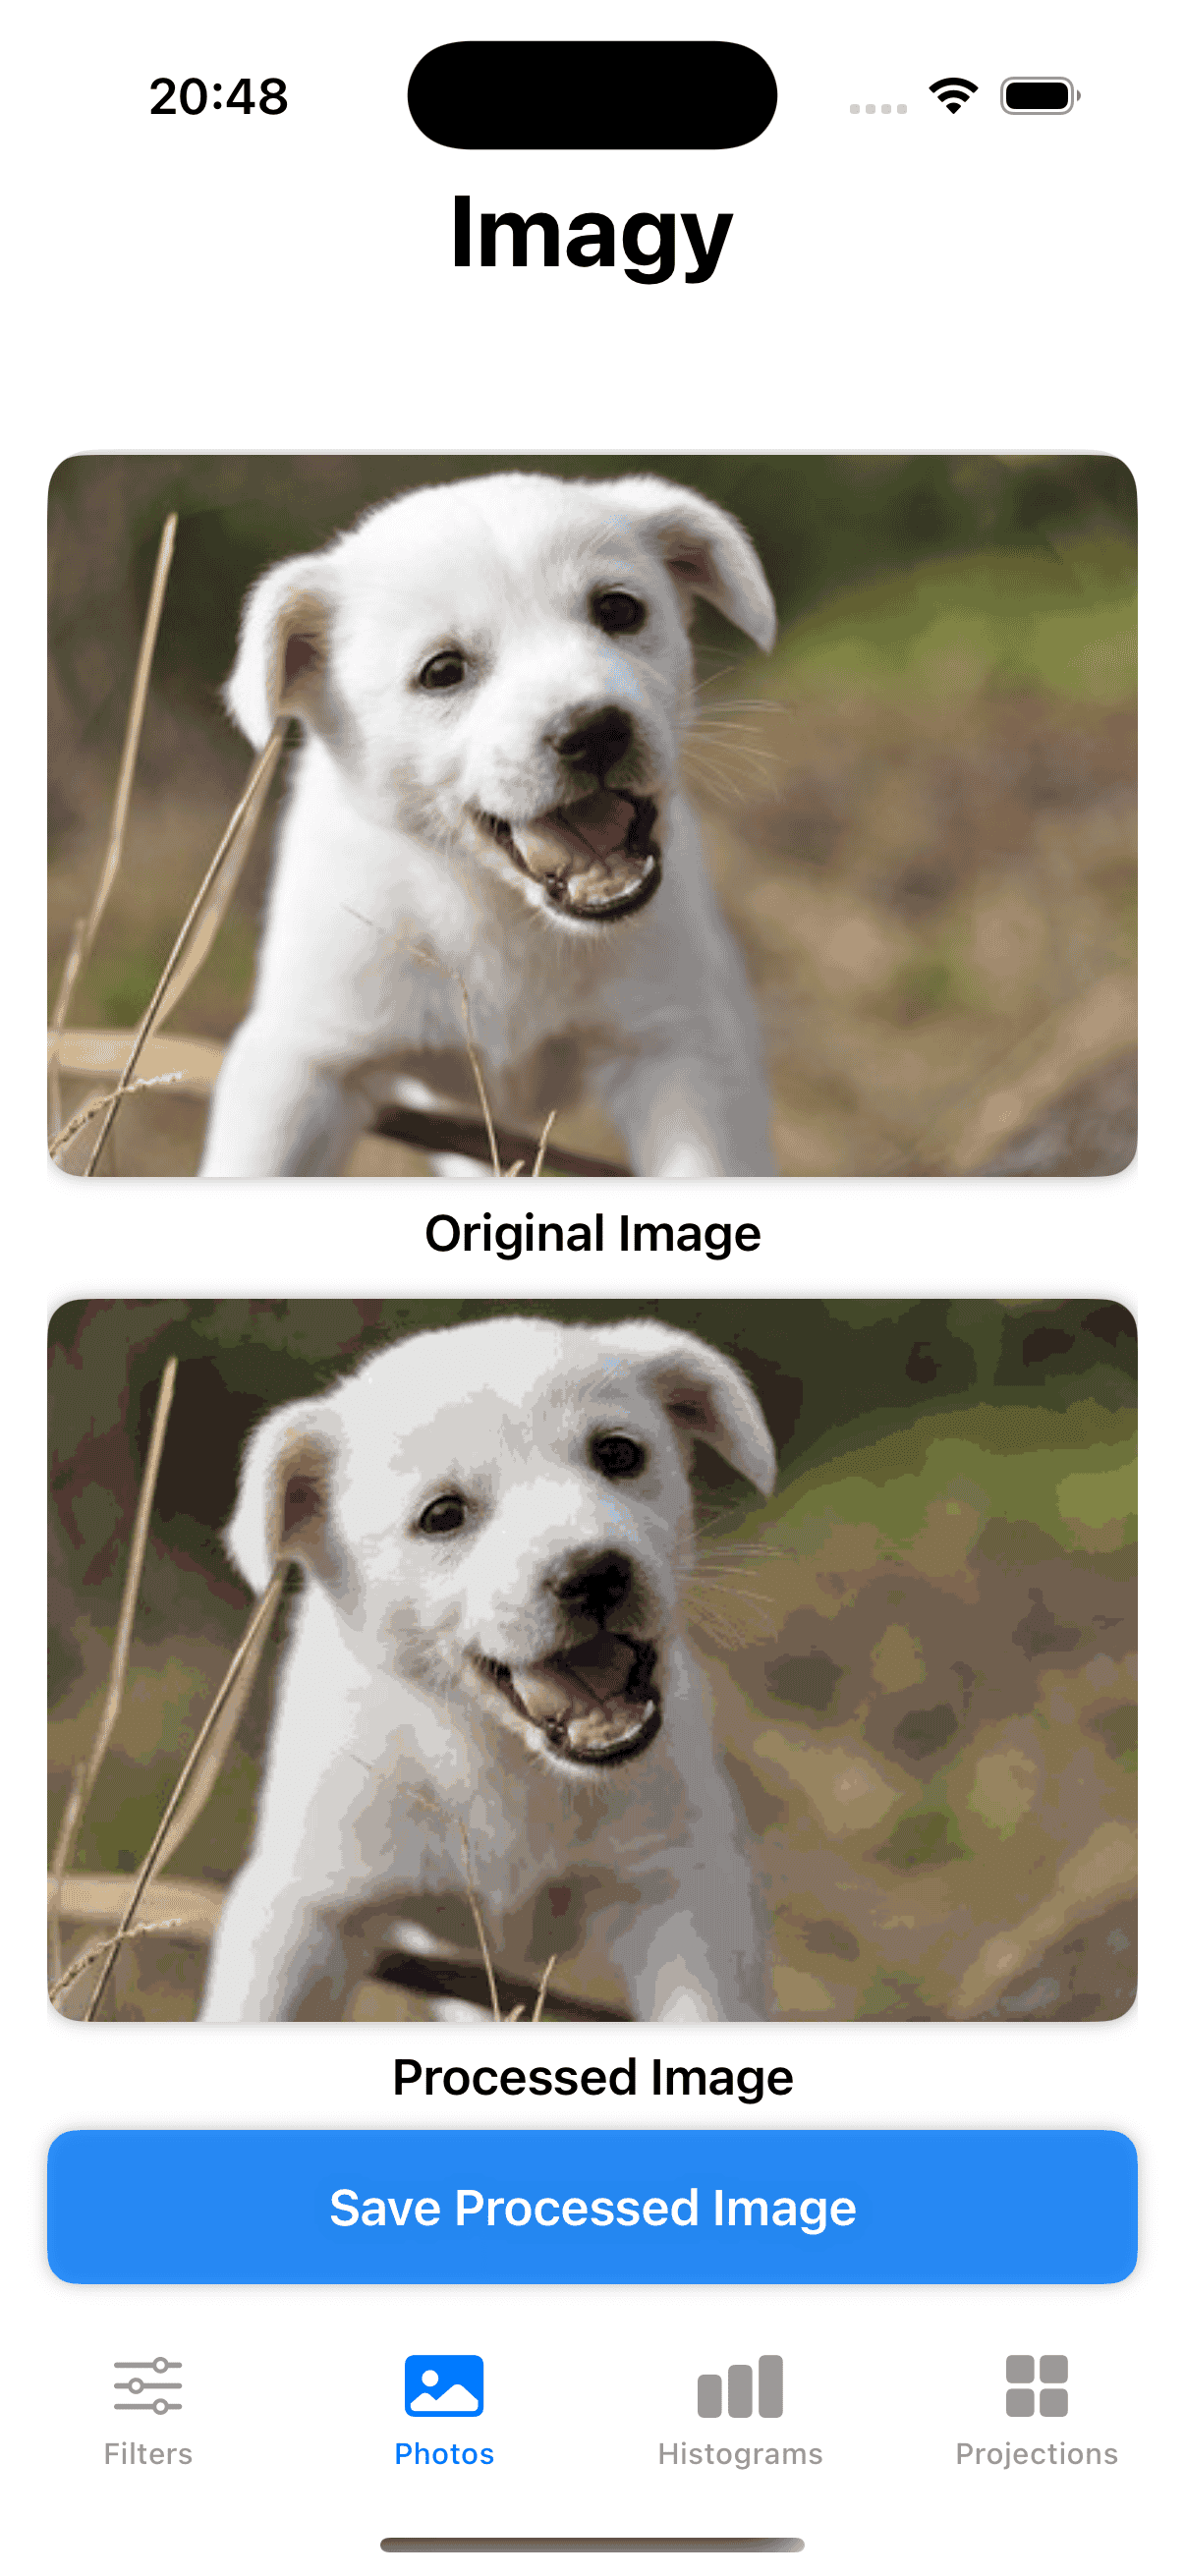
\includegraphics[width=\linewidth]{images/dog_posterize_10.png}
        \caption{levels=10}
        \label{fig:dog_posterize_10}
    \end{subfigure}
    \hfill
    \begin{subfigure}{0.2\textwidth}
        \centering
        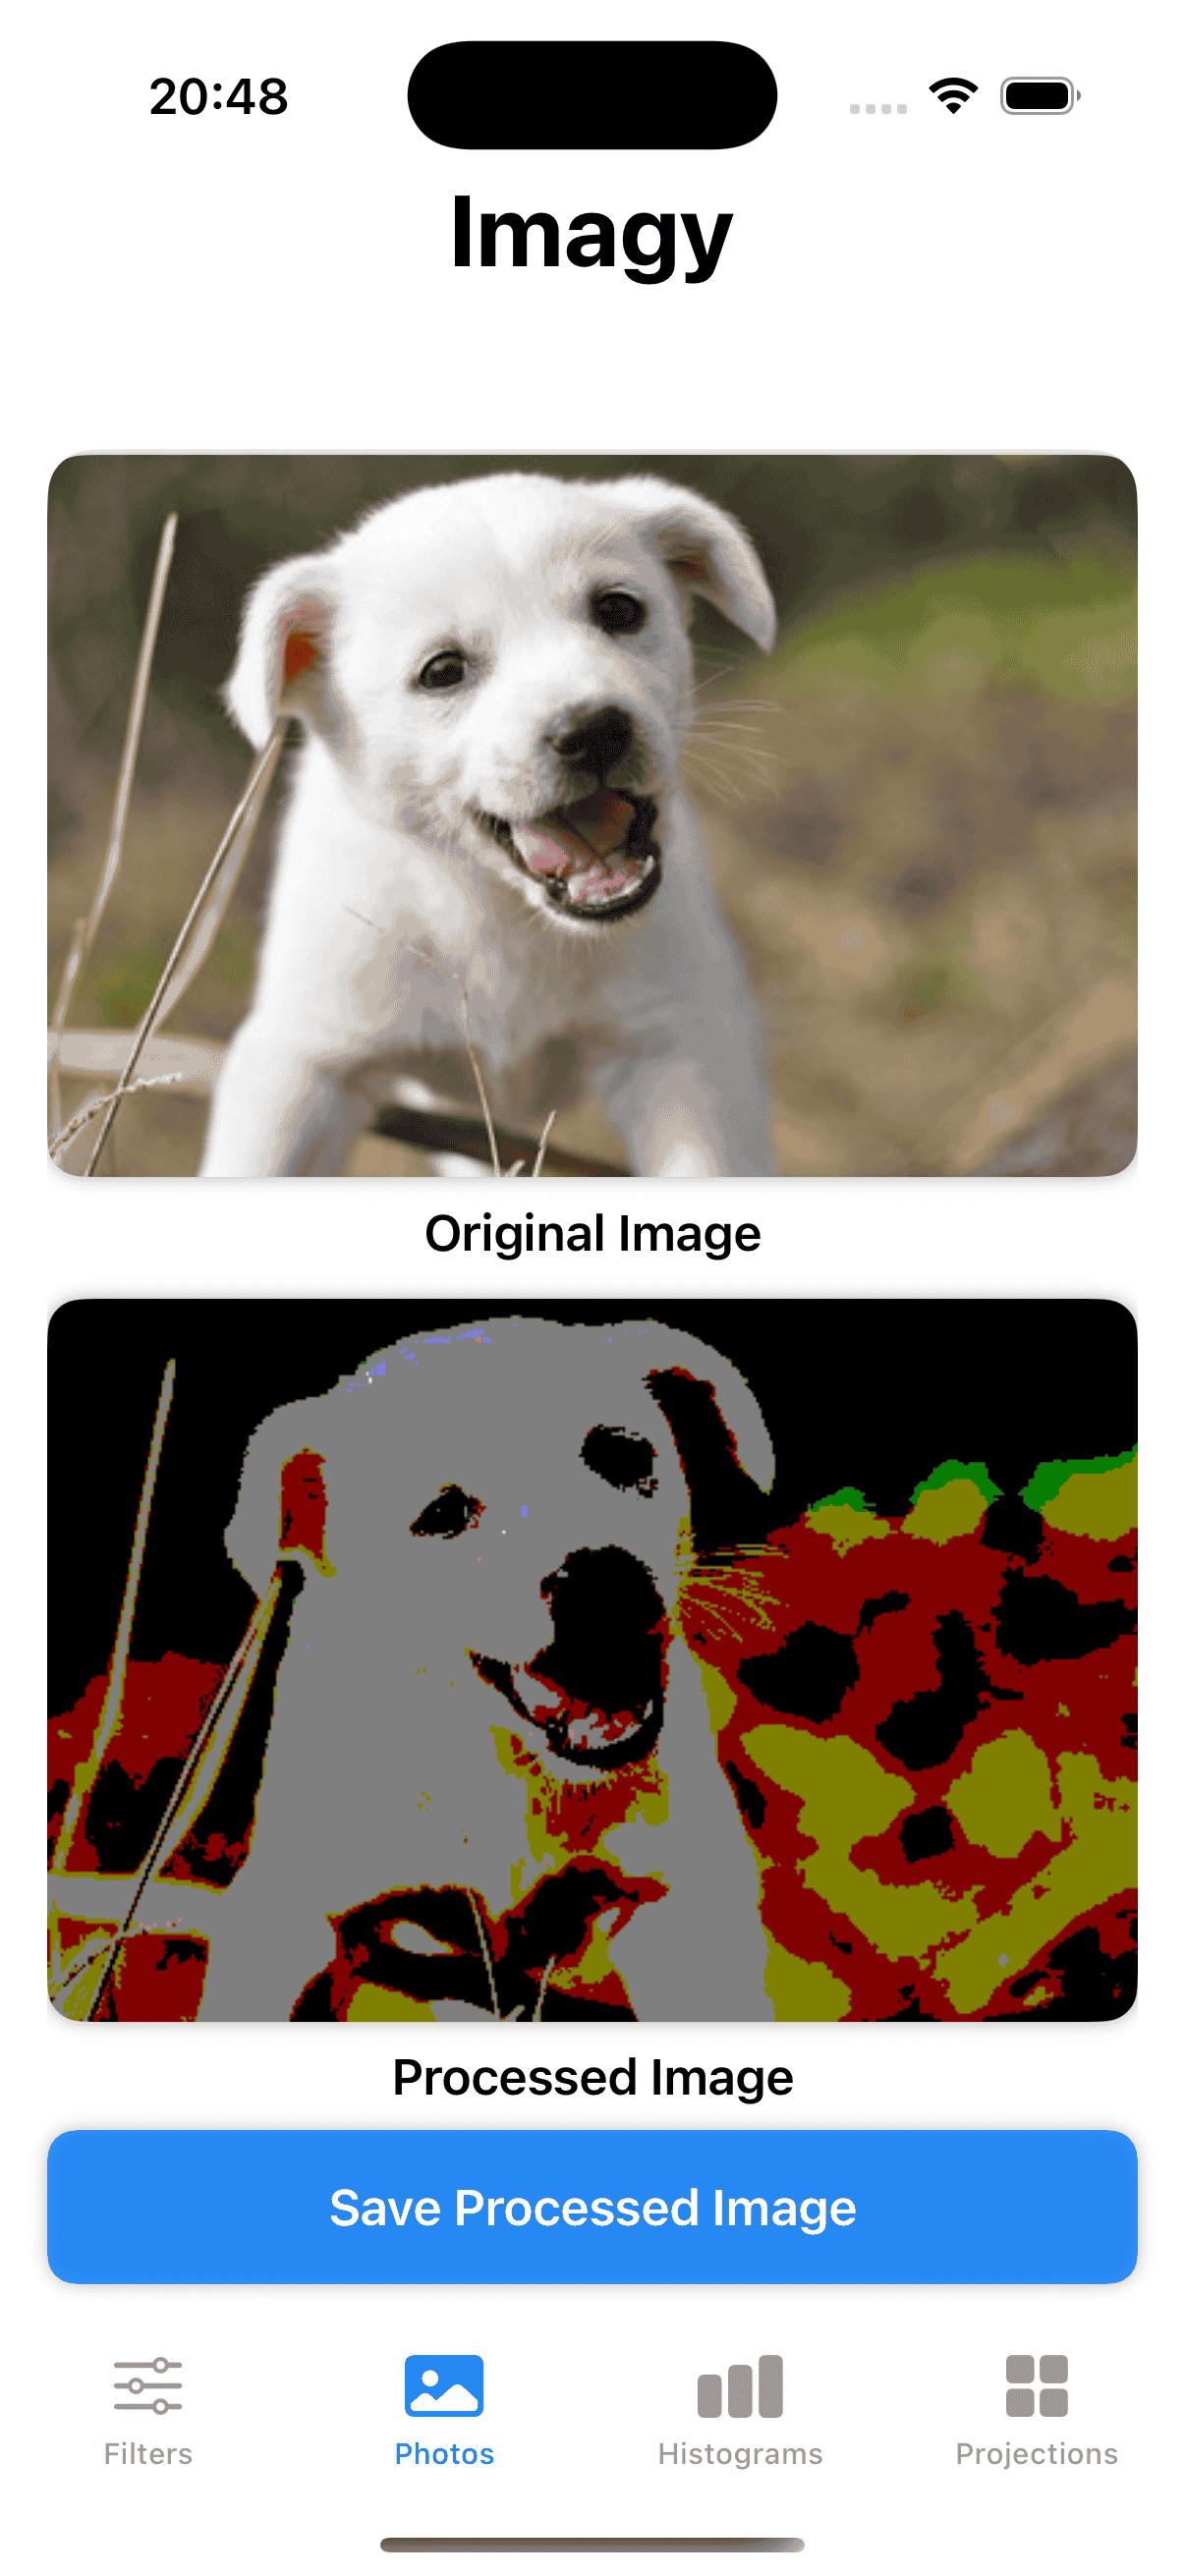
\includegraphics[width=\linewidth]{images/dog_posterize_128.png}
        \caption{levels=128}
        \label{fig:dog_posterize_128}
    \end{subfigure}
    \hfill
    \begin{subfigure}{0.2\textwidth}
        \centering
        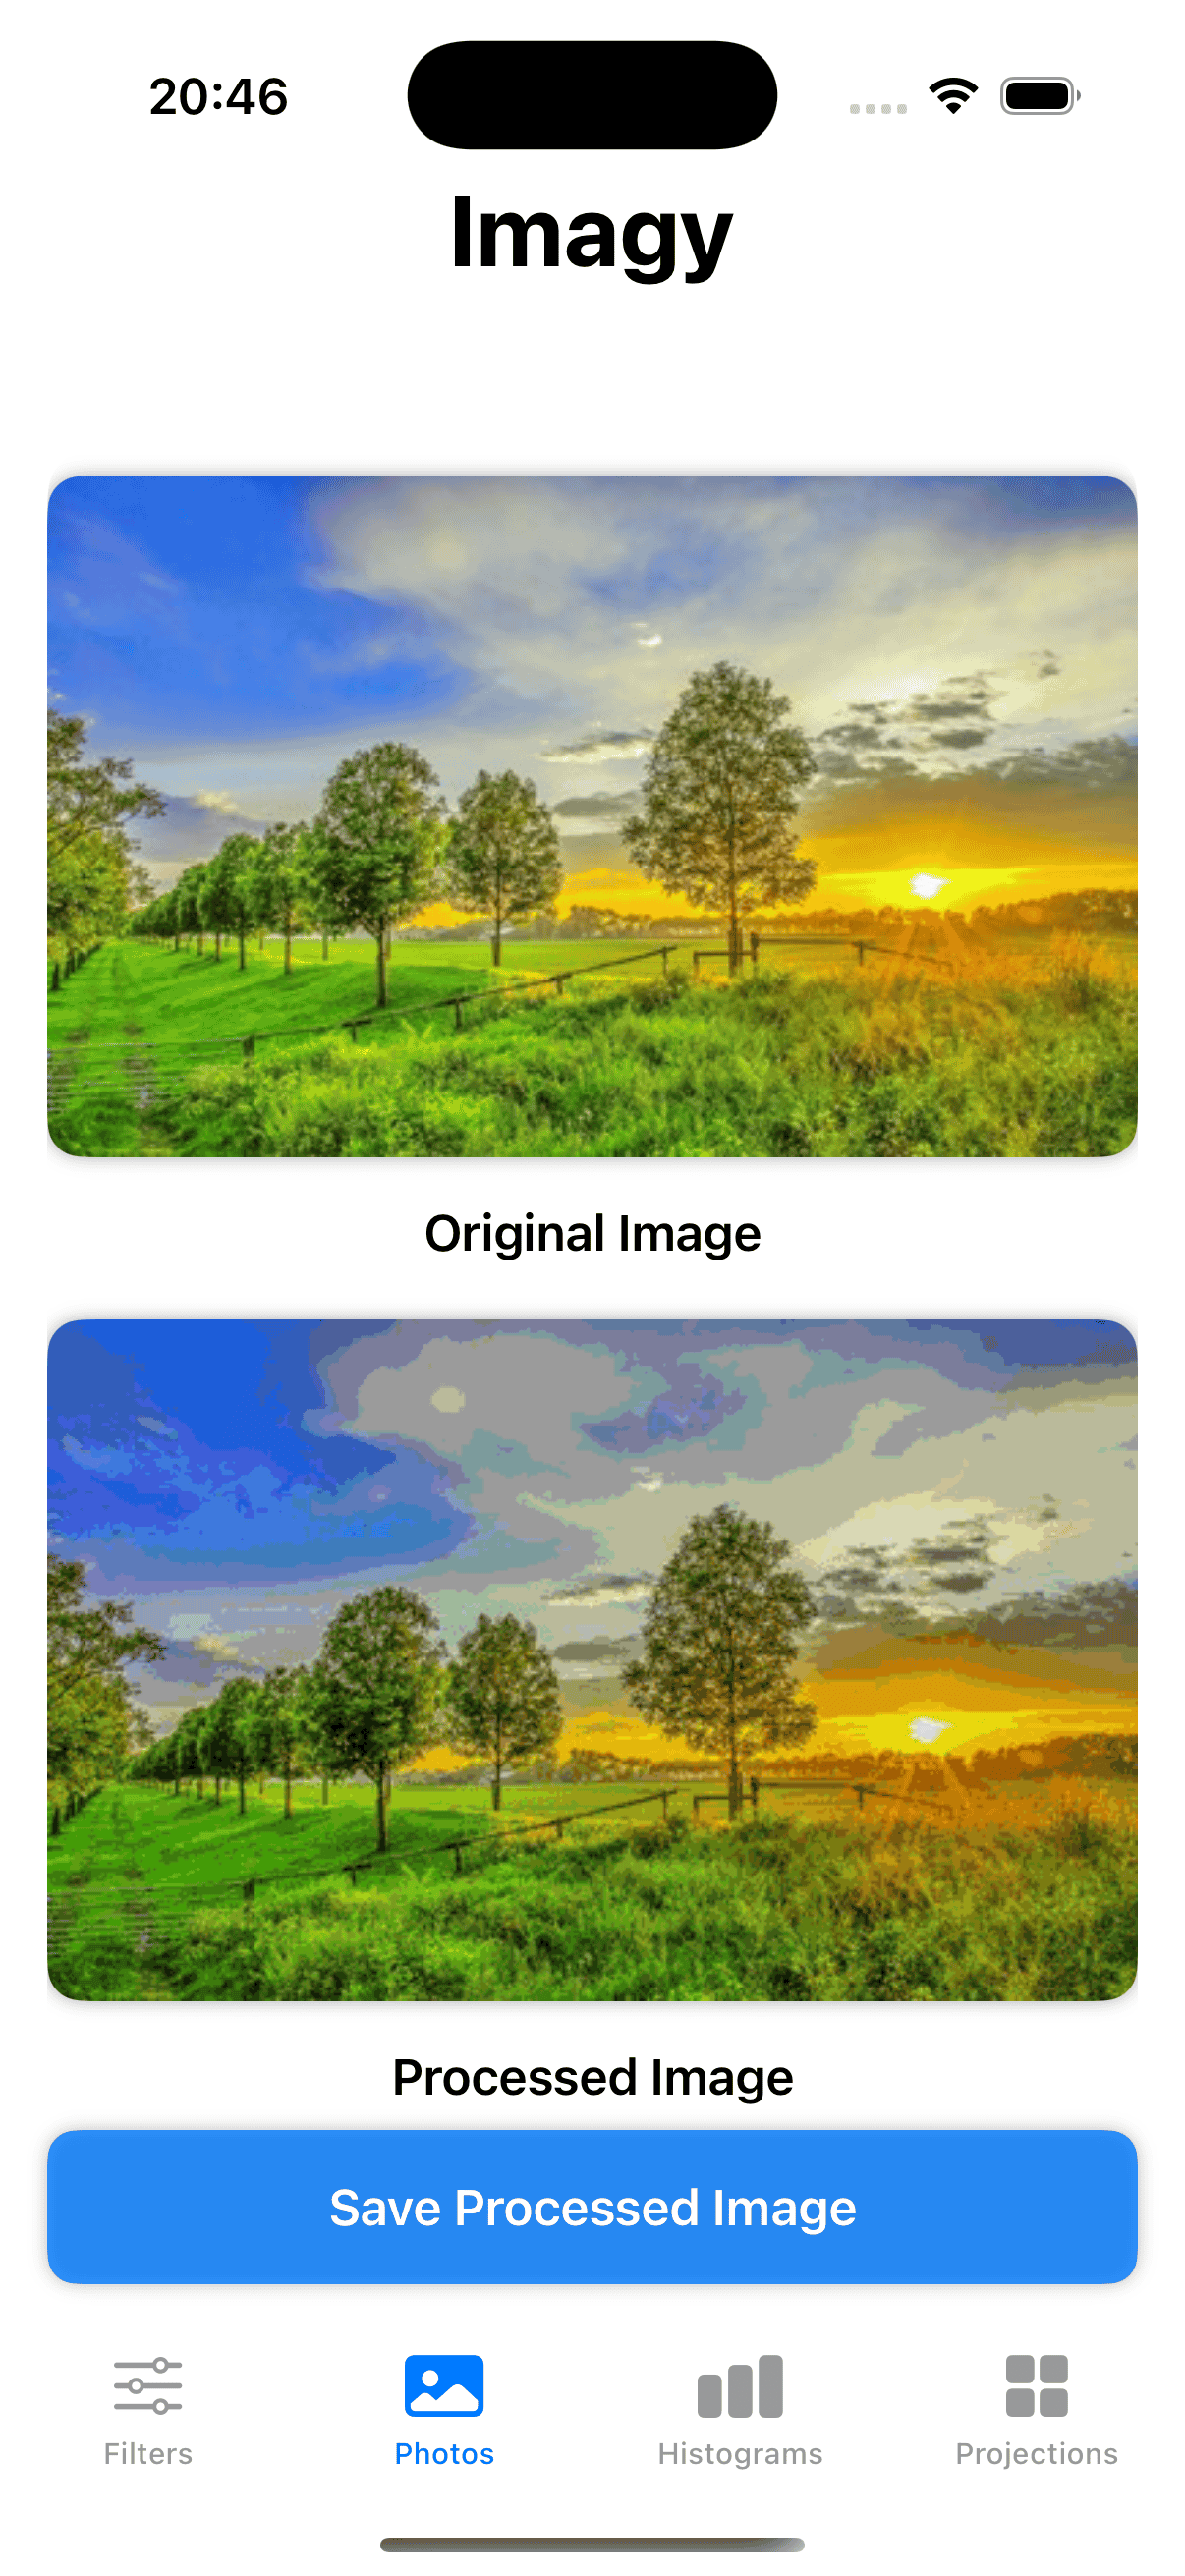
\includegraphics[width=\linewidth]{images/trees_posterize_32.png}
        \caption{levels=32}
        \label{fig:trees_posterize_32}
    \end{subfigure}
    \hfill
    \begin{subfigure}{0.2\textwidth}
        \centering
        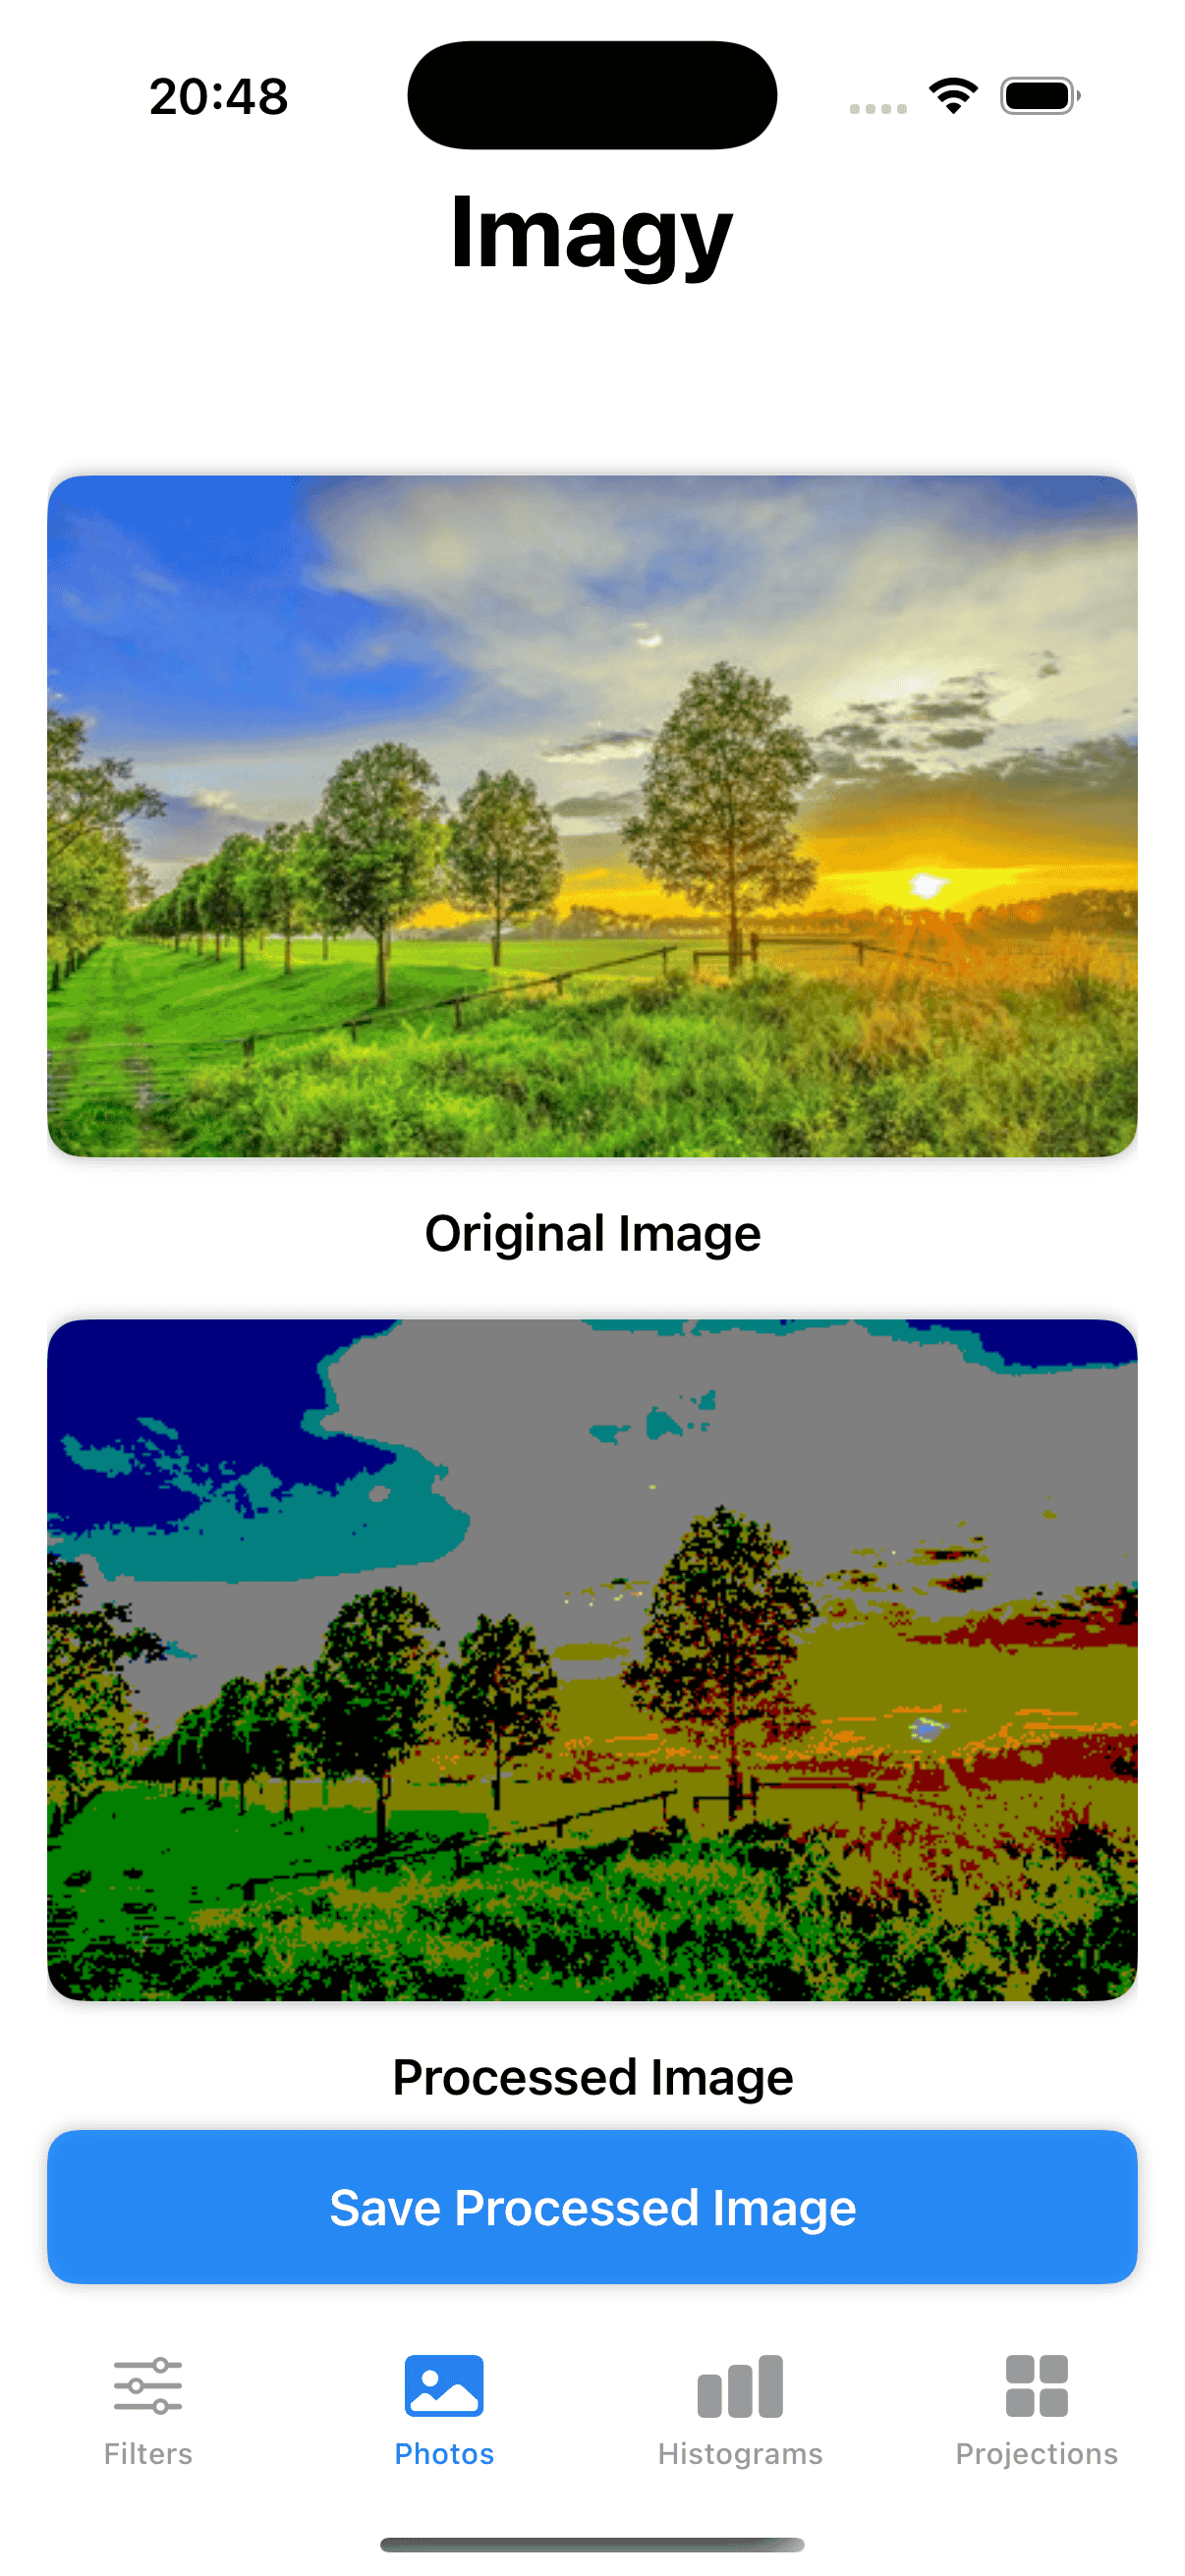
\includegraphics[width=\linewidth]{images/trees_posterize_86.png}
        \caption{levels=86}
        \label{fig:trees_posterize_86}
    \end{subfigure}
    \caption{Posterize filter - demonstracja. Więcej niż $32$ poziomy prowadzą do zdjęć o mocno zniekształconej kolorystyce (i często kształtach), z pominiętymi detalami. $32$ poziomy na zdjęciu \ref{fig:trees_posterize_32} sprawiają, że chmury są bardziej bajkowe. $10$ poziomów na zdjęciu \ref{fig:dog_posterize_10} również zniekształcają tło do sprawiającego wrażenie jakby było modelowane komputerowo przez nieudolnego grafika.}
    \label{fig:posterize}
\end{figure}

\begin{figure}[H]
    \centering
    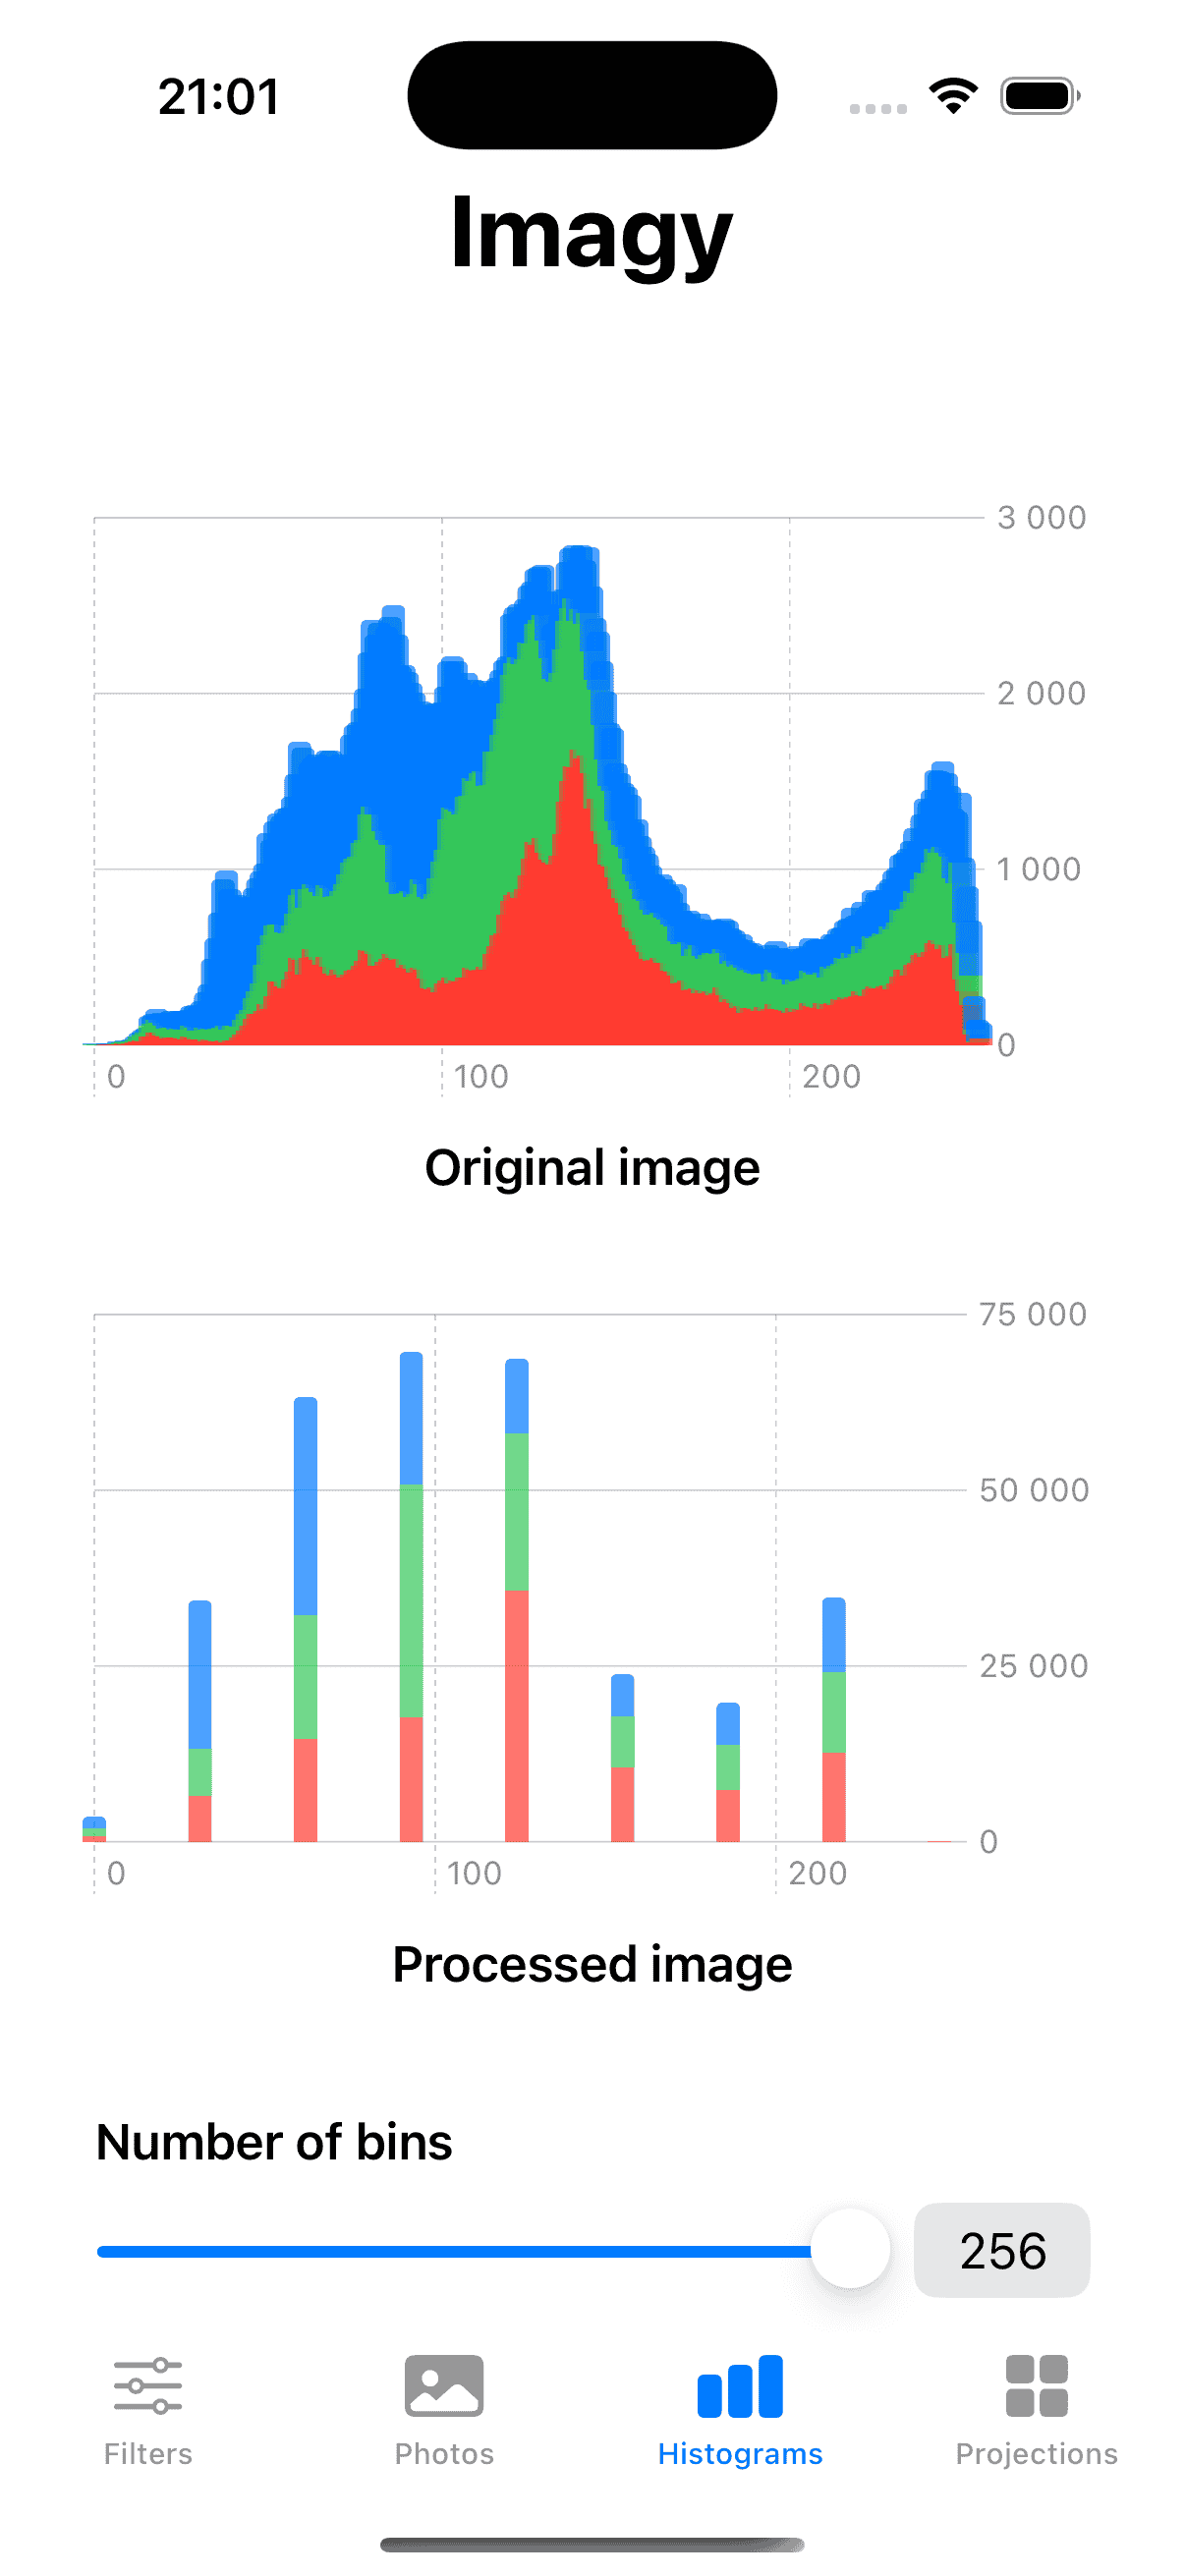
\includegraphics[width=0.25\linewidth]{images/dop_posterize_32_histogram.png}
    \caption{Histogram for dog's posterize filter with levels=32.}
    \label{fig:dop_posterize_32_histogram}
\end{figure}

\subsection{RobertsCross}

\begin{itemize}
    \item \texttt{static var name: String = "Roberts Cross"}
    \item Mając macierze
          $$
              M_1 = \begin{bmatrix}
                  1 & 0  \\
                  0 & -1
              \end{bmatrix}
          $$
          oraz
          $$
              M_2 = \begin{bmatrix}
                  0  & 1 \\
                  -1 & 0
              \end{bmatrix}
          $$
          najpierw przeprowadzamy oddzielnie konwolucję obu tych macierzy na całym obrazku otrzymując $gradientX$ z macierzy $M_1$ oraz $gradientY$ z macierzy $M_2$. Następnie łączymy je (pixel, channel-wise) za pomocą wyliczenia magnitude:
          $$
              N = \text{min}(255, \sqrt{gradXDouble * gradXDouble + gradYDouble * gradYDouble})
          $$
          gdzie $gradXDouble$ jest pikselem z macierzy $gradientX$, $gradYDouble$ jest pikselem z macierzy $gradientY$, a $N$ jest ostateczną wartością po filtrowaniu. Pomaga on wykrywać nagłe zmiany jasności.
    \item Zastosowanie - detekcja krawędzi, segmentacja obrazów, OCR. Często jest używany w Computer Vision zastosowanym do danych medycznych.
\end{itemize}

\begin{figure}[H]
    \centering
    \begin{subfigure}{0.2\textwidth}
        \centering
        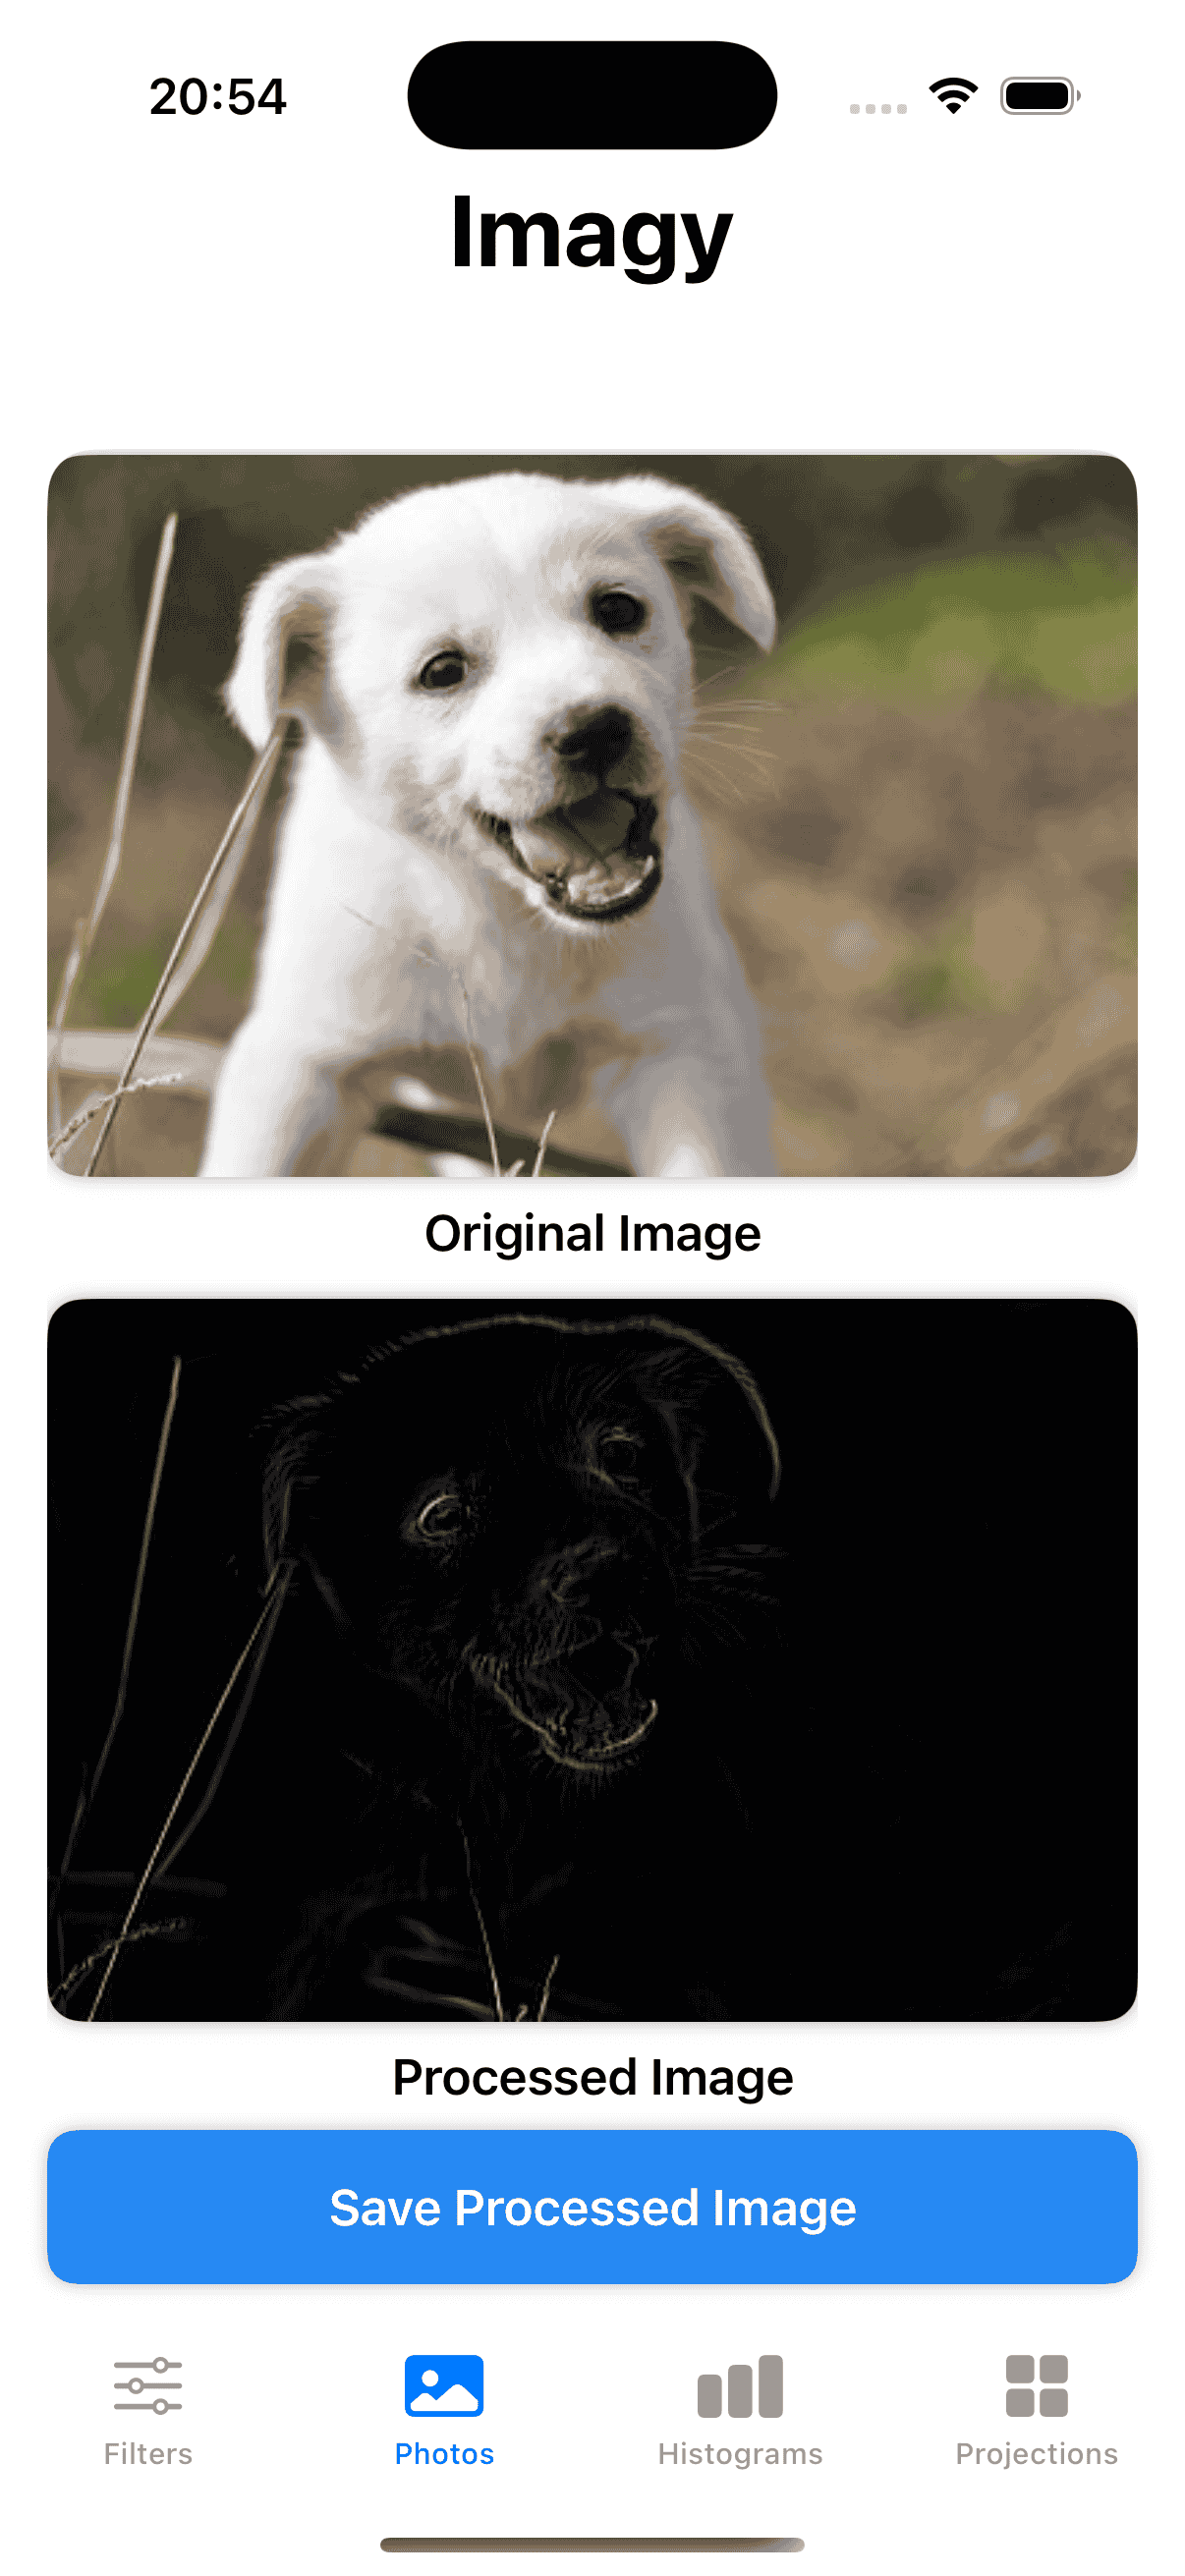
\includegraphics[width=\linewidth]{images/dog_robert_cross.png}
        \label{fig:dog_robert_cross}
    \end{subfigure}
    \hfill
    \begin{subfigure}{0.2\textwidth}
        \centering
        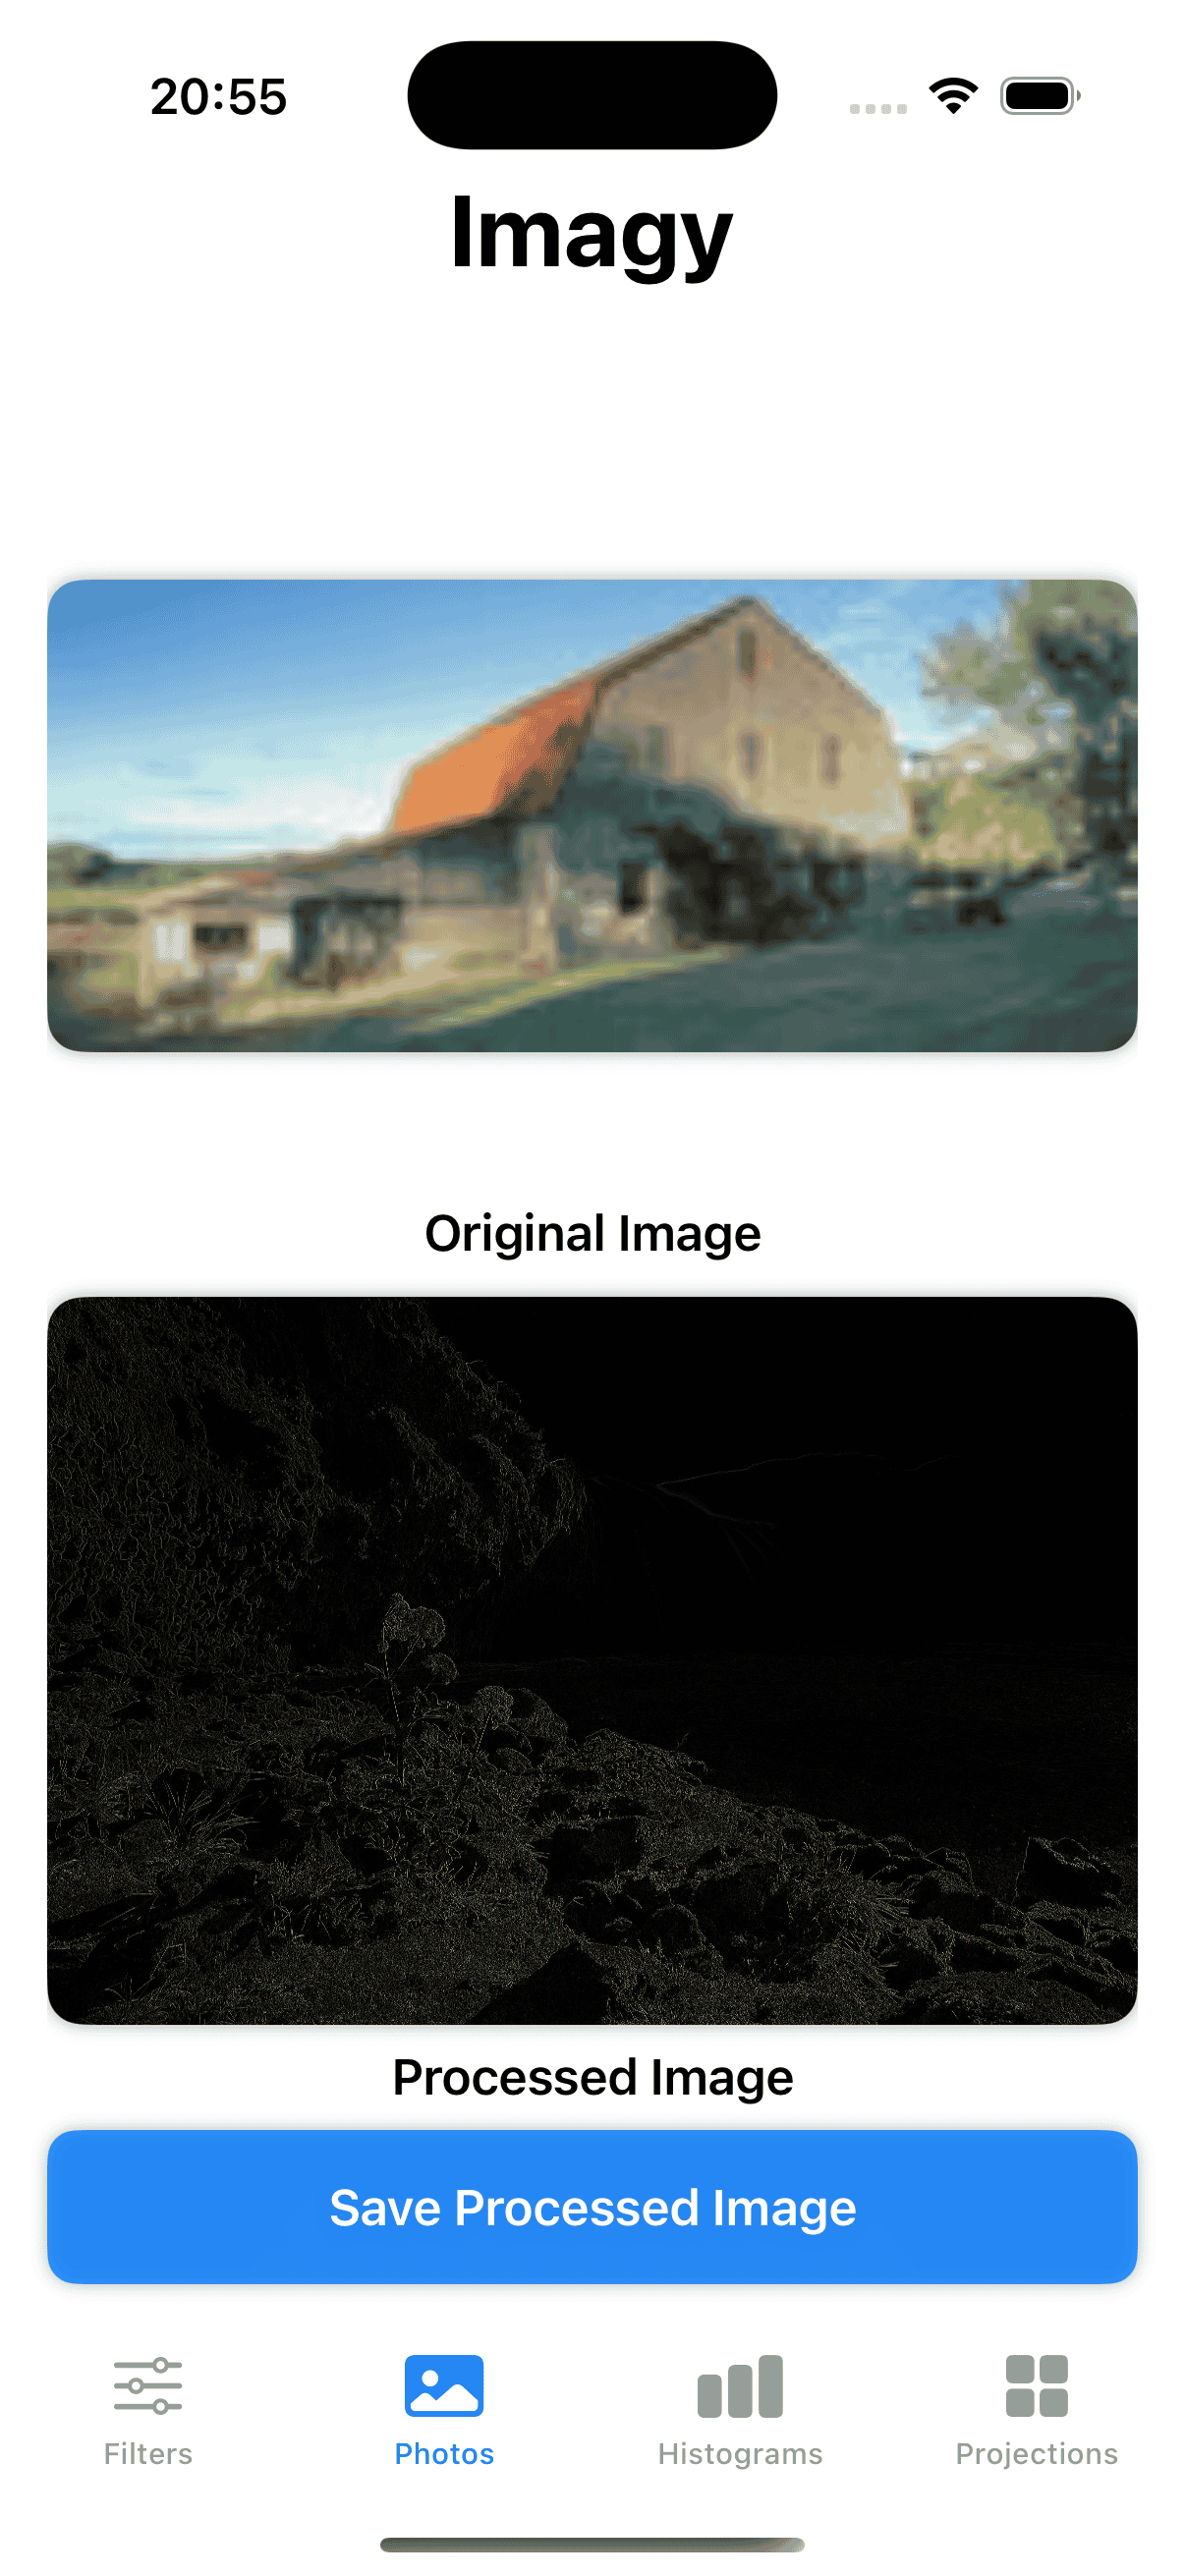
\includegraphics[width=\linewidth]{images/barn_robert_cross.png}
        \label{fig:barn_robert_cross}
    \end{subfigure}
    \hfill
    \begin{subfigure}{0.2\textwidth}
        \centering
        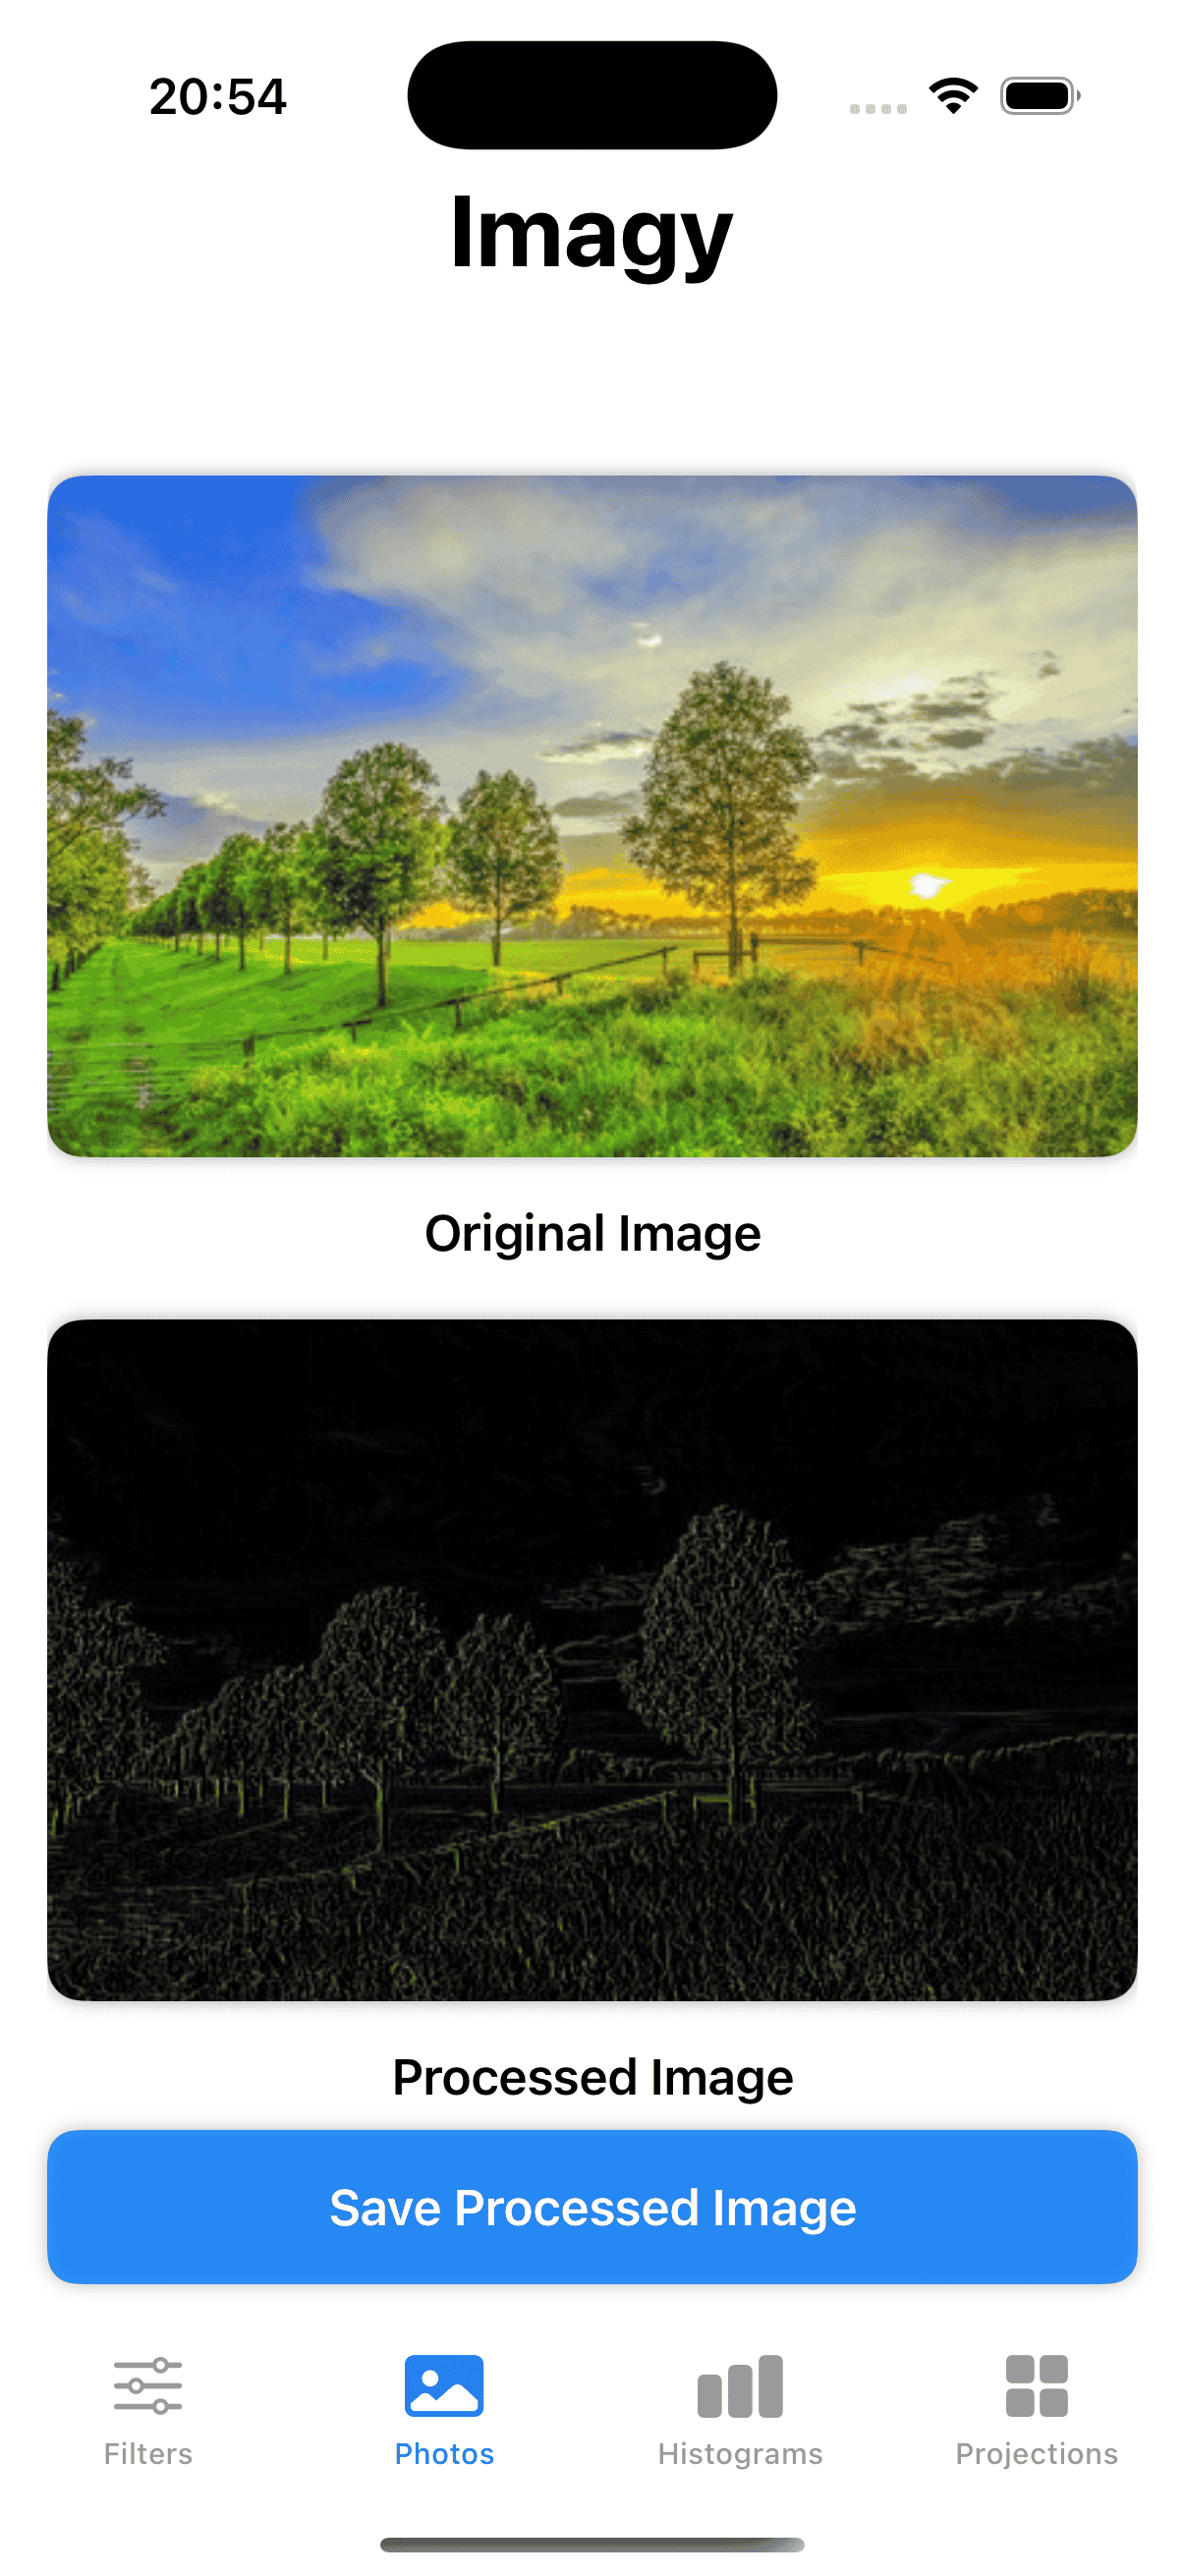
\includegraphics[width=\linewidth]{images/trees_robert_cross.png}
        \label{fig:trees_robert_cross}
    \end{subfigure}
    \caption{Robert Cross filter - demonstracja. Dla zdjęć wyższej rozdzielczości wykrywa poprawnie krawędzie i kontury mniejszych obiektów - w przypadku \ref{fig:trees_robert_cross} konturów chmur nie widzimy po zastosowaniu tego filtru. Komplikacje pojawiają sie dla zdjęc o bardzo małej rozdzielczości - \ref{fig:barn_robert_cross} pokazuje że wtedy filtr ten może zwrócić krawędzie nieznaczącego dla nas szumu.}
    \label{fig:robert_cross}
\end{figure}

\subsection{Saturation}

\begin{itemize}
    \item \texttt{static var name: String = "Saturation"}
    \item \texttt{ adjustment: Double } - nasycenie koloru - wartość $0.0$ prowadzi do koloru szarego, $2.0$ to pełna intensywność. Defaultowo $1.2$, pobierany z widoku GUI ograniczony do wartości z zakresu $0.0-2.0$ z krokiem $0.1$.
    \item Działanie - dla każdego pikselu przeprowadzane są następujące operacje:
          \begin{enumerate}
              \item Wyliczany jest rzut piksela na odcień szarości zgodnie ze wzorem
                    $$
                        let grayValue = 0.299 * Double(pixel.red) + 0.587 * Double(pixel.green) + 0.114 * Double(pixel.blue)
                    $$
              \item Wynikowa wartość po trasformacji wyliczana jest ze wzoru (tutaj dla kanału R, ale wzór analogiczny dla pozostałych):
                    $$
                        newPx.red = UInt8(min(255, max(0, Int(grayValue + adjustment * (Double(oldPx.red) - grayValue)))))
                    $$
          \end{enumerate}
    \item Zastosowanie - fotografia, stylizacja, kinematogradia, gry komputerowe. Zwiększa on intensywność kolorów, wpływając na żywość obrazu.
\end{itemize}

\begin{figure}[H]
    \centering
    \begin{subfigure}{0.2\textwidth}
        \centering
        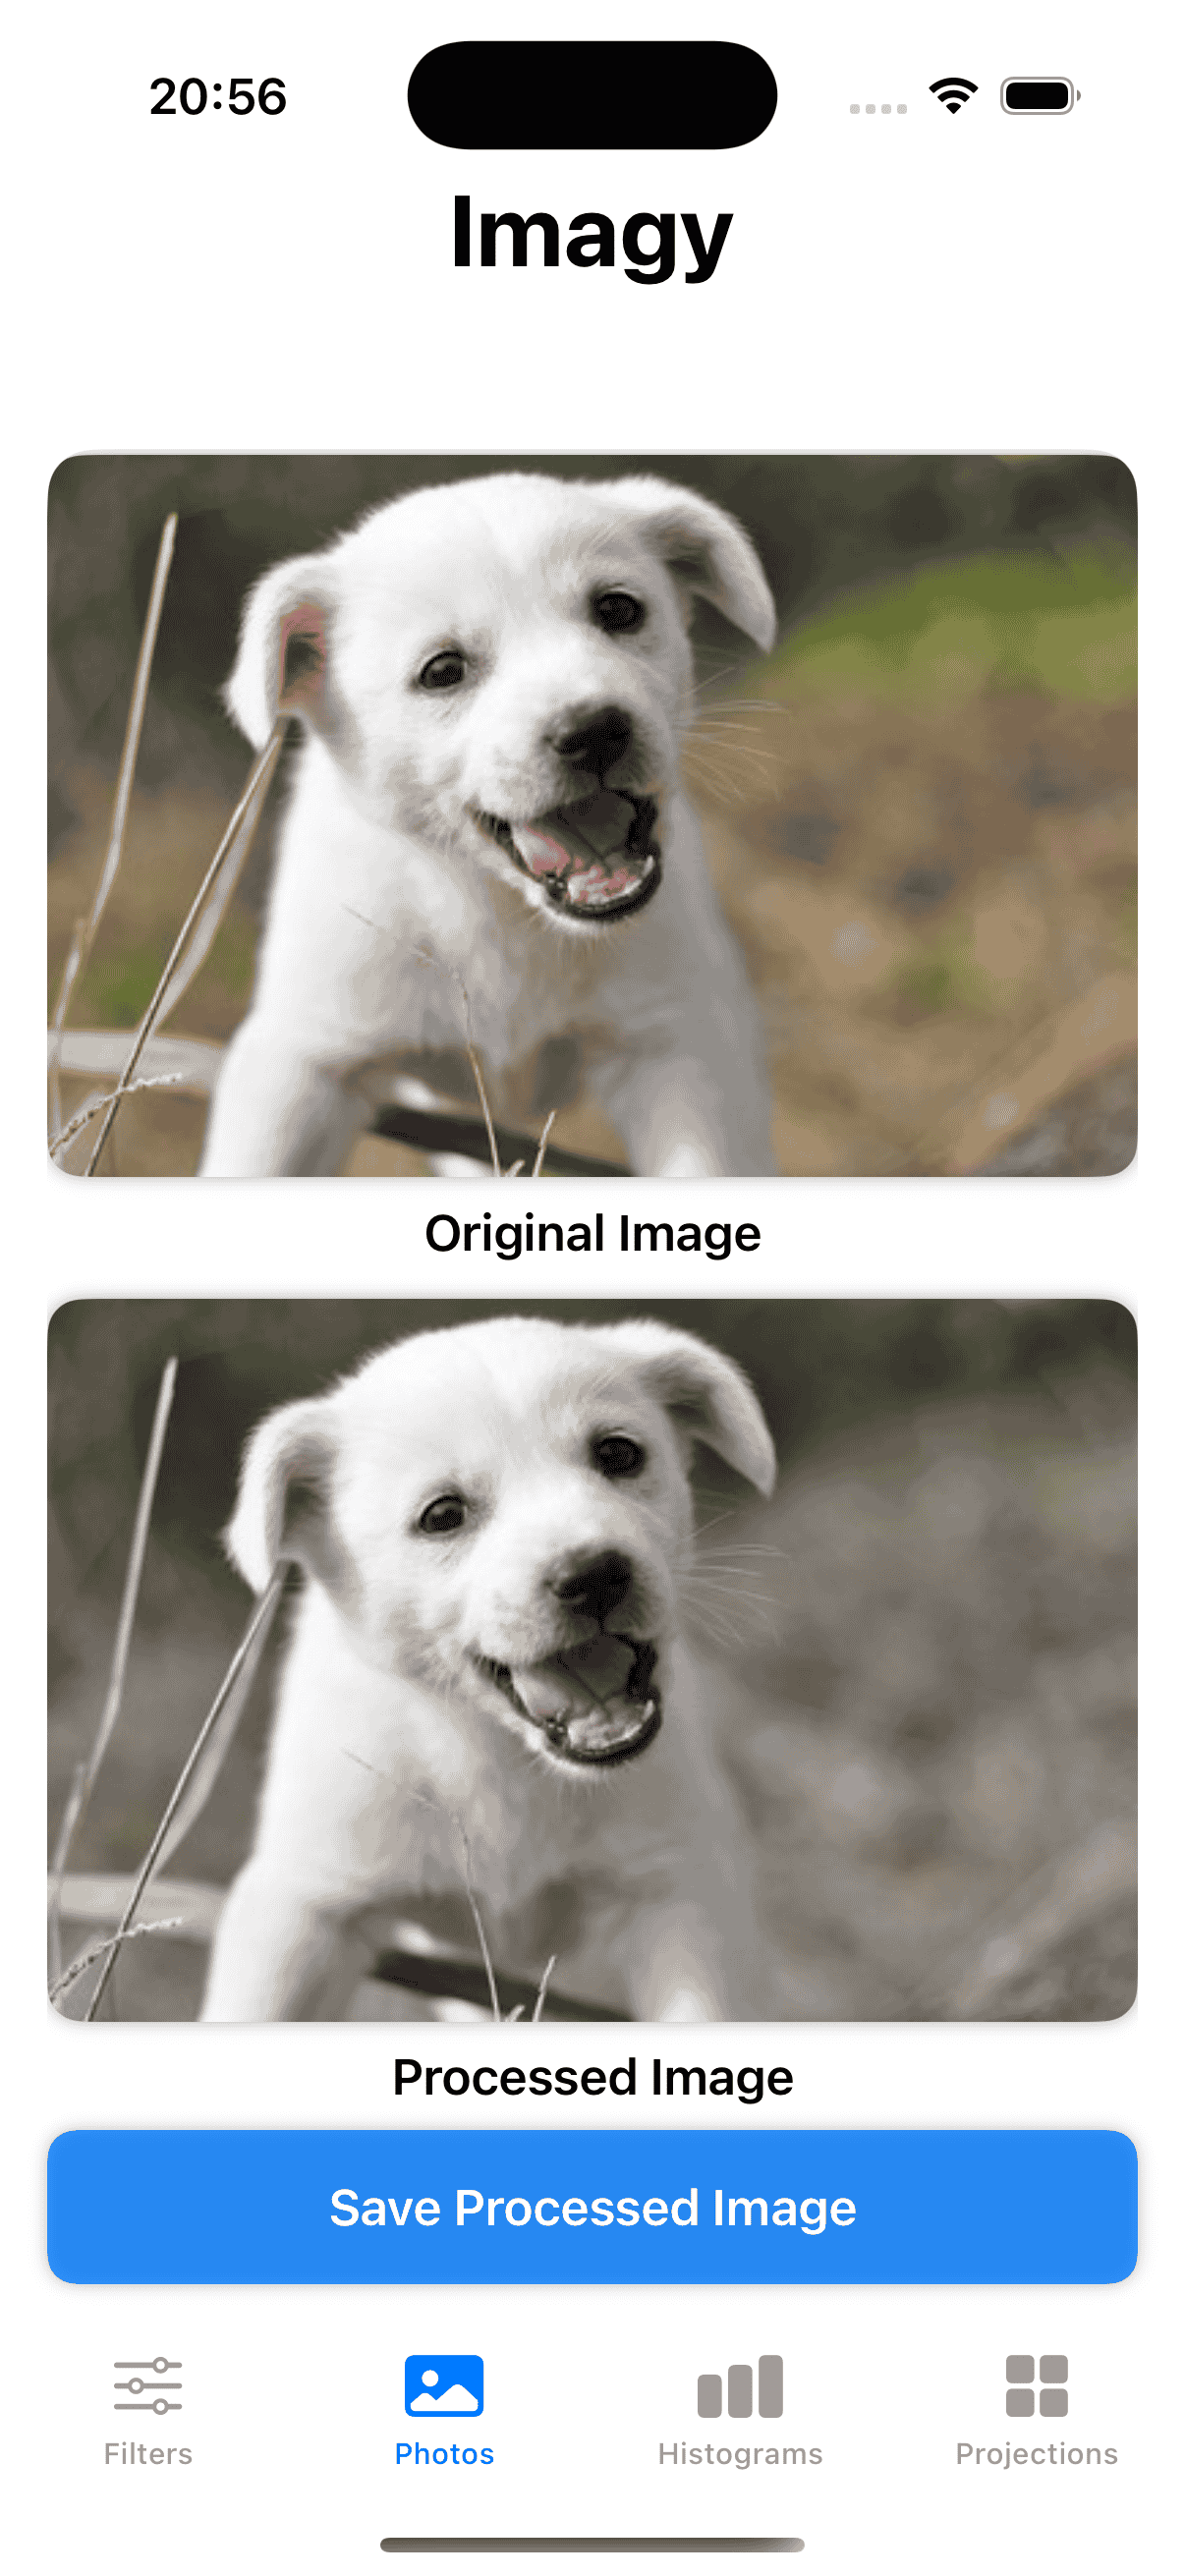
\includegraphics[width=\linewidth]{images/dog_saturation_0.3.png}
        \caption{adjustment=0.3}
        \label{fig:dog_saturation_0}
    \end{subfigure}
    \hfill
    \begin{subfigure}{0.2\textwidth}
        \centering
        \includegraphics[width=\linewidth]{images/dog_saturation_1.7.png}
        \caption{adjustment=1.7}
        \label{fig:dog_saturation_1}
    \end{subfigure}
    \hfill
    \begin{subfigure}{0.2\textwidth}
        \centering
        \includegraphics[width=\linewidth]{images/trees_saturation_1.7.png}
        \caption{adjustment=1.7}
        \label{fig:trees_saturation_1}
    \end{subfigure}
    \hfill
    \begin{subfigure}{0.2\textwidth}
        \centering
        \includegraphics[width=\linewidth]{images/trees_saturation_2.0_historgram.png}
        \caption{adjustment=2.0 - histogram}
        \label{fig:trees_saturation_2}
    \end{subfigure}
    \caption{Saturation filter - demonstracja. Małe wartości adjustment prowadzą do zdjęć "oszarzonych", duże - do zdjęć o podkręconym kolorze, aczkolwiek porównując transformację żywego zdjęcia \ref{fig:trees_saturation_1} do \ref{fig:trees_saturation_1} widzimy w tym drugim bardziej drastyczną zmianę. Z histogramu można wywnioskować, że skrajnie wysoka wartość adjustment ustawia skrajne wartości pikseli dla wielu z kanału B.}
    \label{fig:posterize}
\end{figure}

\subsection{Sepia}

\begin{itemize}
    \item \texttt{static var name: String = "Sepia"}
    \item Działanie - nowe wartości kanałów dla kazdego piksela są wyliczane z następującego wzoru (kolejność RGB):
          \[
              \text{let tr} = 0.393 * Float(pixel.red) + 0.769 * Float(pixel.green) + 0.189 * Float(pixel.blue)
          \]
          \[
              \text{let tg} = 0.349 * Float(pixel.red) + 0.686 * Float(pixel.green) + 0.168 * Float(pixel.blue)
          \]
          \[
              \text{let tb} = 0.272 * Float(pixel.red) + 0.534 * Float(pixel.green) + 0.131 * Float(pixel.blue)
          \]
          gdzie $tr$, $tg$, $tb$ to nowe wartości, przy czym są one potem ograniczane do zakresu $0..255$. Daje to obraz o ciepłych kolorach, nadający klasyczny styl.
    \item Zastosowanie - digitalizacja dokumentów, preprocessing do Computer Vision
\end{itemize}

\begin{figure}[H]
    \centering
    \begin{subfigure}{0.2\textwidth}
        \centering
        \includegraphics[width=\linewidth]{images/trees_sepia.png}
        \label{fig:trees_sepia}
    \end{subfigure}
    \begin{subfigure}{0.2\textwidth}
        \centering
        \includegraphics[width=\linewidth]{images/trees_sepia_hisogram.png}
        \label{fig:trees_sepia_hisogram}
    \end{subfigure}
    \caption{Sepia filter - demonstracja. Zdjęcie wynikowe ma ciepłe, vintage barwy. Potwierdza to histogram o kanale R w skrajnie wysokich wartościach i kanale B o rozkladzie mocno w lewą stronę.}
    \label{fig:sepia}
\end{figure}

\subsection{Sharpening}

\begin{itemize}
    \item \texttt{static var name: String = "Sharpening"}
    \item Działanie - konwolucja z filtrem
          $$
              \begin{bmatrix}
                  0  & -1 & 0  \\
                  -1 & 5  & -1 \\
                  0  & -1 & 0
              \end{bmatrix}
          $$
          - środkowa wartość $5$ zwiększa jasność piksela, otaczające go wartości $-1$ redukują wpływ sąsiednich pikseli. Prowadzi to do zwiększonego konstakstu w miejscach gdzie jasność się zmienia, podkreślając krawędzie.
    \item Zastosowanie - poprawa detali obrazu, OCR
\end{itemize}

\begin{figure}[H]
    \centering
    \begin{subfigure}{0.2\textwidth}
        \centering
        \includegraphics[width=\linewidth]{images/dog_sharpening.png}
        \label{fig:dog_sharpening}
    \end{subfigure}
    \begin{subfigure}{0.2\textwidth}
        \centering
        \includegraphics[width=\linewidth]{images/trees_sharpening.png}
        \label{fig:trees_sharpening}
    \end{subfigure}
    \caption{Sharpening filter - demonstracja. Krawędzie są podkreślone. O ile w przypadku zdjęcia z drzewami generuje to nienaturalnie wyglądający obraz, zdjęcie psa wydaje się być po transformacji dużo bardziej szczegółowe.}
    \label{fig:sharpening}
\end{figure}

\subsection{Sobel}

\begin{itemize}
    \item \texttt{static var name: String = "Sobel"}
    \item Mając macierze
          $$
              M_1 = \begin{bmatrix}
                  -1 & 0 & 1 \\
                  -2 & 0 & 2 \\
                  -1 & 0 & 1
              \end{bmatrix}
          $$
          oraz
          $$
              M_2 = \begin{bmatrix}
                  -1 & -2 & -1 \\
                  0  & 0  & 0  \\
                  1  & 2  & 1
              \end{bmatrix}
          $$
          najpierw przeprowadzamy oddzielnie konwolucję obu tych macierzy na całym obrazku otrzymując $gradientX$ z macierzy $M_1$ oraz $gradientY$ z macierzy $M_2$. Następnie łączymy je (pixel, channel-wise) za pomocą wyliczenia magnitude:
          $$
              N = \text{min}(255, \sqrt{gradXDouble * gradXDouble + gradYDouble * gradYDouble})
          $$
          gdzie $gradXDouble$ jest pikselem z macierzy $gradientX$, $gradYDouble$ jest pikselem z macierzy $gradientY$, a $N$ jest ostateczną wartością po filtrowaniu. Jest to przybliżenie wartości gradientu jasności.
    \item Zastosowanie - detekcja krawędzi, podkreślanie konturów.
\end{itemize}

\begin{figure}[H]
    \centering
    \begin{subfigure}{0.2\textwidth}
        \centering
        \includegraphics[width=\linewidth]{images/dog_sobel.png}
        \label{fig:dog_sobel}
    \end{subfigure}
    \hfill
    \begin{subfigure}{0.2\textwidth}
        \centering
        \includegraphics[width=\linewidth]{images/barn_sobel.png}
        \label{fig:barn_sobel}
    \end{subfigure}
    \hfill
    \begin{subfigure}{0.2\textwidth}
        \centering
        \includegraphics[width=\linewidth]{images/trees_sobel.png}
        \label{fig:trees_sobel}
    \end{subfigure}
    \caption{Sobel filter - demonstracja. W porównaniu z \ref{fig:robert_cross} wykrywane jest dużo więcej krawędzi, również dla zdjęć o małej rozdzielczości (co niewątpliwie można traktować jako zaletę względem tamtego). Krawędzie są jednak grupsze, w przypadku wysoce szczegółowych obszarów szybciej się zlewają.}
    \label{fig:sobel}
\end{figure}

\subsection{Vignett}

\begin{itemize}
    \item \texttt{static var name: String = "Vignette"}
    \item Każdy piksel, każdy kanał wyliczany zgodnie ze wzorem:
          \begin{enumerate}
              \item Liczymy odległość piksela od środka obrazu.
              \item Każdą z wartstw koloru mnożymy przez ten sam współczynnik obliczany ze wzoru
                    $$
                        \text{let intensityFactor} = 1.0 - min(distance / maxDistance, 1.0) * intensity
                    $$
                    i ograniczamy do zakresu $0...255$.
          \end{enumerate}
    \item Należy wspomnieć że jest to jedna z wielu alternatywnych (i raczej prostsza) implementacja tego fitra, np. transformacja sugerowana przez Chat GPT to wyliczanie intensywności z eksponenty z gęstości rozkładu normalnego (tutaj z dodatkowymi hiperparametrami).
    \item Filtr powoduje stopniowe (w rozumiemie odlegości od środka obrazka) przyciemnianie.
    \item Zastosowanie - efekty artystyczne, kinematografia, rozpoznawanie wzorców (skupienie modelu na środku obrazka).
\end{itemize}

\begin{figure}[H]
    \centering
    \begin{subfigure}{0.2\textwidth}
        \centering
        \includegraphics[width=\linewidth]{images/trees_vignette.png}
        \label{fig:dog_sobel}
    \end{subfigure}
    \hfill
    \begin{subfigure}{0.2\textwidth}
        \centering
        \includegraphics[width=\linewidth]{images/dog_vignette.png}
        \label{fig:barn_sobel}
    \end{subfigure}
    \hfill
    \begin{subfigure}{0.2\textwidth}
        \centering
        \includegraphics[width=\linewidth]{images/trees_vignette.png}
        \label{fig:trees_sobel}
    \end{subfigure}
    \caption{Vignett filter - demonstracja. Im dalej od środka obrazu, tym bardziej przyciemnione są zdjęcia. Potwierdza to histogram na prawo, reprezentujący rozkład pikseli przekształconego zdjęcia psa widocznego na środkowym rysunku.}
    \label{fig:vingnett}
\end{figure}

\section{Histogram}

Dla każdego kanału, dla każdej wartości piksela ($0...255$), zliczamy liczbę pikseli w obrazku o tej wartości. Wynik przedstawiamy w postaci barplota.

\begin{figure}[H]
    \centering
    \begin{subfigure}{0.2\textwidth}
        \centering
        \includegraphics[width=\linewidth]{images/histogram_26.png}
        \label{fig:histogram_26}
    \end{subfigure}
    \hfill
    \begin{subfigure}{0.2\textwidth}
        \centering
        \includegraphics[width=\linewidth]{images/histogram_95.png}
        \label{fig:histogram_95}
    \end{subfigure}
    \hfill
    \begin{subfigure}{0.2\textwidth}
        \centering
        \includegraphics[width=\linewidth]{images/histogram_256.png}
        \label{fig:histogram_256}
    \end{subfigure}
    \caption{Prezentacja działania histogramu dla tego samego zdjęcia (filtr negatyw na dole), różne ilości binów (widoczne na screenach).}
    \label{fig:histogram}
\end{figure}

\section{Rzuty}

Niech obraz poddawany transformacji ma wymiar $x*y*3$, gdzie ostatni wymiar reprezentuje 3 kanały koloru.

\subsection{Pionowy}
Jest on sumą wartości pikseli w każdym wierszu, z podziałem na kanały koloru. Prowadzi nas to do wektora jednowymiarowego rozmiaru $y*3$

\subsection{Poziomy}
Jest on sumą wartości pikseli w każdej kolumnie, z podziałem na kanały koloru. Prowadzi nas to do wektora jednowymiarowego rozmiaru $x*3$

\begin{figure}[H]
    \centering
    \begin{subfigure}{0.2\textwidth}
        \centering
        \includegraphics[width=\linewidth]{images/rzuty_horizontal.png}
        \label{fig:rzuty_horizontal}
    \end{subfigure}
    \begin{subfigure}{0.2\textwidth}
        \centering
        \includegraphics[width=\linewidth]{images/rzuty_vertical.png}
        \label{fig:rzuty_vertical}
    \end{subfigure}
    \caption{Rzuty pionowe i poziome demonstracja działania narzędzia. Liczba binów histogramu to liczba pikseli w danym wymiarze obrazka. Którego rzutu screen dotyczy da się bezpośrednio z niego wyczytać.}
    \label{fig:rzuty}
\end{figure}

\section{Pozostałe funkcjonalności}

Detale implementacyjne pozostałych funkcjonalności udokumentowane są kodem, nie zostaną tutaj szczegółowo opisane jako iż Swift nie jest tematem przewodnim tego projektu. Prócz funkcjonalności przedstawionych w ramach opisu filtrów Imagy pozwala również na:

\begin{itemize}
    \item Wczytywanie obrazku do przetworzenia bezpośrednio z galerii (applowe Photos).
    \item Zapisywanie przetworzonego obrazu do wcześniej wspomnianych Photos.
\end{itemize}

\begin{figure}[H]
    \centering
    \begin{subfigure}{0.2\textwidth}
        \centering
        \includegraphics[width=\linewidth]{images/loading.png}
        \caption{Ekran ładowania. Logo wygenerowane przez AI.}
        \label{fig:home}
    \end{subfigure}
    \begin{subfigure}{0.2\textwidth}
        \centering
        \includegraphics[width=\linewidth]{images/image_choice.png}
        \caption{Ekran startowy. Kliknięcie w górny "No Picture" przenosi do widoku ładowania zdjęcia. Zdjęcia załadowane można podmienić w ten sam sposób, tj kliknięcie wyższego (aka oryginalnego) zdjęcia przeniesie do widoku ładowania}
        \label{fig:image_load}
    \end{subfigure}
    \begin{subfigure}{0.2\textwidth}
        \centering
        \includegraphics[width=\linewidth]{images/home.png}
        \caption{Ekran startowy z załadowanym zdjęciem. Tutaj bez filtrów, zatem oba są takie same.}
        \label{fig:home}
    \end{subfigure}
    \begin{subfigure}{0.2\textwidth}
        \centering
        \includegraphics[width=\linewidth]{images/image_load.png}
        \caption{Widok ładoania zdjęcia.}
        \label{fig:image_load}
    \end{subfigure}
    \label{fig:home_screen}
\end{figure}

\begin{figure}[H]
    \centering
    \begin{subfigure}{0.2\textwidth}
        \centering
        \includegraphics[width=\linewidth]{images/filter_choice.png}
        \caption{Dropdown z możliwymi filtrami do wybrania. Wybór filtru automatycznie wywołuje renderowanie widoku z jego dodatkowymi ustawieniami oraz (oprócz Custom Filter, który ma przycisk $Apply$) automatyczne nakładanie filtru na obrazek w tle.}
        \label{fig:filter_choice}
    \end{subfigure}
    \hfill
    \begin{subfigure}{0.2\textwidth}
        \centering
        \includegraphics[width=\linewidth]{images/filter_options_1.png}
        \caption{Opcje customizacji zachodania filtru - suwak wyboru. Zgodnie z wcześniej wspomnianym działaniem w sekcji \ref{Filtry} nie pozwala na wybór z continuum lecz tylko na skok o wskazanej dokładności}
        \label{fig:filter_options_1}
    \end{subfigure}
    \hfill
    \begin{subfigure}{0.2\textwidth}
        \centering
        \includegraphics[width=\linewidth]{images/filter_options_2.png}
        \caption{Opcje customizacji zachodania filtru - dropdown wyboru.}
        \label{fig:filter_options_2}
    \end{subfigure}
    \caption{Wszelkie powyżej wspomniane funkcjonalności wyboru filtrów są zablokowane na czas przeliczania danych przez aplikację w tle, wtedy są wyświetlane z mniejszą alphą. Dotyczy to operacji aplikowania filtru na zdjęcie, liczenia histogramu oraz rzutów pionowych.}
    \label{fig:filter_screen}
\end{figure}

\section{Podsumowanie}

\textbf{Imagy} jest nowoczesną aplikacją na iOS, spełniającą wszelkie zalecenia Apple odnośnie pisania nowoczesnych, futurystycznych i skalowalnych aplikacji (z wyjątkiem poniżej wspomnianego mankamentu obliczeniowego wynikającego z ograniczeń narzuconych odgórnie na projekt). Implementuje ona kilkanaście podstawowych filtrów powszechnie używanych w fotografi, Computer Vision czy filmografii. Pozwala na zapis i odczyt zdjęć bezpośrednio z urządzenia oraz analizę zmian dokonanych przez daną transformację wewnątrz aplikacji zarówno przez wizualne porównanie zdjęć, jak i poprzez porównanie rozkładu ich pikseli z pomocą rzutu pionowego, poziomego i histogramu.

Aplikacja jest przeznaczona do celów edukacyjnych, powinna być urzywana jedynie ze zdjęciami niskiej rozdzielczości.

\section{Ograniczenia}

Z powodu ograniczeń czasowych następujące funkcjonalności nie zostały zaimplementowane:
\begin{itemize}
    \item \textbf{Wsparcie dla zdjęć wysokiej jakości (np. 4K)} - istniejąca implementacja ze względu na potrzeby nakładania filtrów 'from scratch' jest zbyt wolna. Wszelkie transformacje są wykonywane na jednym wątku CPU, co sprawia że na urządzeniach mobilnych zdjęcia o rozdzielczości przekraczającej 480p wymagają długich czasów obliczeń, powodując zauważalne opóźnienia.
    \item \textbf{Możliwość nakładania wielu filtrów na jedno zdjęcie} - ze względu na wcześniej wspomniany problem optymalizacyjny oraz duży nakład czasowy wymagający dostosowania GUI do wielu filtrów, została zaimplementowana tylko możliwość zastosowania pojedynczego filtru.
    \item \textbf{Dostęp do większej liczby filtrów.} - z powodu ograniczeń czasowych i przejrzystości systemu, zostały zaimplementowane tylko podstawowe filtry (w liczbie 19).
    \item \textbf{Wyrównywanie histogramu.}
\end{itemize}

\section{Dodatek}

Opisany powyżej projekt ze względu na potrzebę zapakowania w GUI pochłonął masę czasu właśnie na ten jego aspekt, skutecznie zmniejszając pulę przeznaczoną na naukę i poszukiwania innych ciekawych metod (oraz ograniczając zaimplementowane do tych wpasowujących się w napisany User Interface). W ramach ciekawostki i rozwinięcia części filtrów tutaj opisanych przekierowuję do (niekompletnej) pracy napisanej przezemnie jakiś czas temu - \href{https://github.com/Pawlo77/Computer-Vision/tree/main/processing}{Computer Vision - Processing}.

\end{document}